\documentclass[letterpaper,10pt]{book}
% Change to 10 pt
\usepackage{pdfpages}
\usepackage{morewrites}			% to counteract the no write space problem
\setcounter{tocdepth}{6}

\usepackage[framemethod=TikZ]{mdframed}

\usepackage{fancyhdr}

\usepackage{paralist}
\usepackage{amsmath}
\usepackage{amsfonts}
\usepackage{amssymb}
\usepackage{graphicx}

\usepackage{datetime}
%\usepackage{ulem}

%\usepackage[nottoc]{toobibind}

\usepackage[inline]{enumitem}

% Outer margin at 2.50 is exacty correct to fit the ``corruption alert'' tables
\usepackage[inner=1.0in, outer=2.50in, top=2.54cm,bottom=2.54cm, marginparwidth=2.25in]{geometry}

\usepackage{marginnote}
\usepackage{longtable}
\usepackage{booktabs}
\usepackage{xcolor}

\usepackage{soul}

%%%%%%%%%%%%
\definecolor{ForestGreen}{rgb}{0.00,0.29,0.098}
%%%%%%%%%%%%

\usepackage{marginnote}

\usepackage{imakeidx} 
\usepackage[
	backref=true,
	style=numeric,
%	citestyle=numeric,
	backend=bibtex
	]{biblatex}
\usepackage[driverfallback=hypertex,colorlinks=True]{hyperref}
\usepackage{cleveref}

\makeindex[name=scripture,columnsep=20pt, columnseprule=True,columns=3, title=Scripture References]
\makeindex[name=speaker,columnsep=20pt, columnseprule=True,,columns=2, title=Sermon Creator]
\makeindex[name=series,columnsep=20pt, columnseprule=True,,columns=2, title=Sermon Series]
\makeindex[name=date,columnsep=20pt, columnseprule=True,columns=2, title=Sermon Date]
\makeindex[name=event,columnsep=20pt, columnseprule=True,columns=2, title=Event]
\makeindex[name=topic,columnsep=20pt, columnseprule=True,columns=2, title=Topic]
\makeindex[name=AWIP,columnsep=20pt, columnseprule=True,columns=3, title=All Words in Passage]
\makeindex[name=NWIV,columnsep=20pt, columnseprule=True,columns=3, title=Number of Words in Verse]
\makeindex[name=PNIP,columnsep=20pt, columnseprule=True,columns=3, title=Proper Names in Passage]
\makeindex[name=PEIP,columnsep=20pt, columnseprule=True,columns=2, title=Prophetic Events in Passage]
\makeindex[name=TWPAQ,columnsep=20pt, columnseprule=True,columns=1, title=13-Word Phrases and Quotes]
\makeindex[name=PFTTIS,columnsep=20pt, columnseprule=False,columns=3, title=Phrases found 13 times in scripture]
\makeindex[name=WFTTIS,columnsep=20pt, columnseprule=False,columns=3, title=Words found 13 times in scripture]
\makeindex[name=WFITV,columnsep=20pt, columnseprule=False,columns=3, title=Words found in exactly 13 verses]
\makeindex[name=EVENTS,columnsep=20pt, columnseprule=False,columns=2, title=Sermon Log by Place]
\makeindex[name=QUESTIONS,columnsep=20pt, columnseprule=False,columns=2, title=Bible Questions]
\makeindex[name=DOCTRINES,columnsep=20pt, columnseprule=False,columns=2, title=Doctrines]
\makeindex[name=SONGS,columnsep=20pt, columnseprule=False,columns=1, title=Songs]
\makeindex[name=LOCATION,columnsep=20pt, columnseprule=False,columns= 2, title=Location]
\makeindex[name=FACEBOOK,columnsep=20pt, columnseprule=False,columns=2, title=Facebook]
\makeindex[name=DEVOTIONAL,columnsep=20pt, columnseprule=False,columns=2, title=Devotional Items]
%%%%%%%%%%%%%%%%% EXTRA COLORS
\definecolor{champagne}{rgb}{0.97,0.91,0.81}
\definecolor{bone}{rgb}{0.89,0.85,0.79}
\pagestyle{fancy}
\fancyhf{}
\fancyhead[LE,RO]{\today}
\fancyhead[RE,LO]{Daily Bible Reading}
\fancyhead[CE,CO]{-page \thepage  - }

\fancyfoot[CO,CE]{\leftmark}
%\fancyfoot[LE,RO]{CSCE 692, HW1}

\title{DBR\\
Daily \\ Reads}
\author{Keith Anthony \\
\today }
%+/ffffff +   \pagenumbering{gobble}
\bibliography{Bibliographies/All20220122}

\setlength{\fboxsep}{1.0pt}

\usepackage[utf8]{inputenc}
\usepackage{tikz}

\begin{document}
%%%%%%%%%%%% Tile Page

\begin{titlepage}

\begin{flushright}
\rightskip=-2.5cm
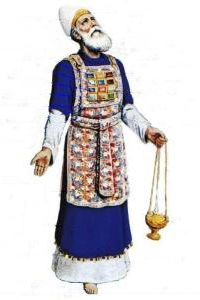
\includegraphics[width=50mm,scale=1.5]{Extras/Melchisedec.jpg}
\vspace{0.4in}  % Create a title for the document and write it in bold font
\LARGE{\textbf{\date}} % Again, do a line break
\linebreak 
% Create a subtitle \large{with Outlines, Statistics, Cross References, and Notes}
\vspace{0.5in}
\begin{flushleft}
\LARGE{Day \#106: Saturday, 16 April 2022  \\}\vspace{0.25in}
\LARGE{1 Kings 16-18 Psalm 119:49-56 Proverb 16}
\end{flushleft}
\vspace{0.6in}
\bigskip

\normalsize{Xenia, Oh.\\}
\normalsize{created: \today}
\vspace{1.3in}

\end{flushright}
\end{titlepage}

\newpage 
\tableofcontents\hypertarget{TOC}{}
\listoffigures
\listoftables

\hyphenation{A-bim-e-lech bre-thren E-phra-im  Gib-e-o-nites Jer-u-sa-lem through-out Phil-i-stines The-o-phil-us Am-a-le-kites ven-geance Mesh-el-e-mi-ah onan-ism Phar-a-oh thoughts grev-ous-ness Hach-a-liah adul-ter-er Shad-rach}

%%%%%%%%%%%%%%%%% EXTRA COLORS
%%%%%%%%%%%%%%%%% EXTRA COLORS
%%%%%%%%%%%%%%%%% EXTRA COLORS
\definecolor{champagne}{rgb}{0.97,0.91,0.81}
\definecolor{bone}{rgb}{0.89,0.85,0.79}

\definecolor{ForestGreen}{rgb}{0.00,0.29,0.098}
\definecolor{GIVING}{cmyk}{1,0.0,0.72,.1}

\definecolor{MLPE}{cmyk}{1,1,0,.45}
\definecolor{SOCCER}{cmyk}{.77, 0, .42, .49}
\definecolor{PAYBILL}{cmyk}{0,0.83,0.76,0.07}
\definecolor{SERMON}{cmyk}{.14,.9,0,.30} % aka seance \href{http://www.flatuicolorpicker.com/purple-cmyk-color-model/}{seance}
\definecolor{BIBLE}{cmyk}{0,.17,.74,.17}
\definecolor{WORKBLUE}{cmyk}{1, .5, 0, .6}
\definecolor{myOrange}{cmyk}{0, .4, .98, .03}
\definecolor{myTan}{cmyk}{0.0,.07,.17,.10}
\definecolor{myRed}{cmyk}{0,1,1,0}
\definecolor{myWhite}{cmyk}{0,0,0,0}
\definecolor{BLUESoD}{cmyk}{.97,.84,0,.04}
\definecolor{WHITE}{cmyk}{0,0,0,0}
\definecolor{OLDGOLD}{cmyk}{0.05,0.3,1.00,0}
\definecolor{CASTLETON}{cmyk}{1,0,0.31,0.66}
\definecolor{cadmiumgreen}{rgb}{0.0, 0.42, 0.24}
\definecolor{jungle}{rgb}{0.203,0.4882,0.1718}
\definecolor{MYGOLD}{rgb}{1,.84,0}

\definecolor{MYLIGHTGRAY}{rgb}{.85,.85,.85}

\definecolor{codegreen}{rgb}{0,0.6,0}
\definecolor{codegray}{rgb}{0.5,0.5,0.5}
\definecolor{codepurple}{rgb}{0.58,0,0.82}
\definecolor{backcolour}{rgb}{0.95,0.95,0.92}


\mdfdefinestyle{MyFrame}{%
    linecolor=blue,
    outerlinewidth=2pt,
    roundcorner=5pt,
    innertopmargin=\baselineskip,
    innerbottommargin=\baselineskip,
    innerrightmargin=10pt,
    innerleftmargin=10pt,
    backgroundcolor=gray!25!white}


\mdfdefinestyle{MyFrame2}{%
    linecolor=black,
    outerlinewidth=2pt,
    roundcorner=5pt,
    innertopmargin=\baselineskip,
    innerbottommargin=\baselineskip,
    innerrightmargin=10pt,
    innerleftmargin=10pt,
    backgroundcolor=yellow!25!white}


%%%%%
%% for PFTTIS list
%%%%%

%%% And Joseph said unto
\index[PFTTIS]{And Joseph said unto!Genesis!Gen 40:008}
\index[PFTTIS]{And Joseph said unto!Genesis!Gen 40:012}
\index[PFTTIS]{And Joseph said unto!Genesis!Gen 41:025}
\index[PFTTIS]{And Joseph said unto!Genesis!Gen 42:014}
\index[PFTTIS]{And Joseph said unto!Genesis!Gen 42:018}
\index[PFTTIS]{And Joseph said unto!Genesis!Gen 44:015}
\index[PFTTIS]{And Joseph said unto!Genesis!Gen 45:003}
\index[PFTTIS]{And Joseph said unto!Genesis!Gen 45:004}
\index[PFTTIS]{And Joseph said unto!Genesis!Gen 46:031}
\index[PFTTIS]{And Joseph said unto!Genesis!Gen 48:009}
\index[PFTTIS]{And Joseph said unto!Genesis!Gen 48:018}
\index[PFTTIS]{And Joseph said unto!Genesis!Gen 50:019}
\index[PFTTIS]{And Joseph said unto!Genesis!Gen 50:024}


%%% a shadow
\index[PFTTIS]{a shadow!1Chronicles!1Chr 029:15}
\index[PFTTIS]{a shadow!Job!Job 008:09}
\index[PFTTIS]{a shadow!Job!Job 014:02}
\index[PFTTIS]{a shadow!Job!Job 017:07}
\index[PFTTIS]{a shadow!Psalm!Psa 102:011}
\index[PFTTIS]{a shadow!Psalm!Psa 144:004}
\index[PFTTIS]{a shadow!Ecclesiastes!Eccl 006:012}
\index[PFTTIS]{a shadow!Ecclesiastes!Eccl 008:013}
\index[PFTTIS]{a shadow!Isaiah!Isa 04:006}
\index[PFTTIS]{a shadow!Isaiah!Isa 25:004}
\index[PFTTIS]{a shadow!Jonah!Jnh 04:06}
\index[PFTTIS]{a shadow!Colossians!Col 02:017}
\index[PFTTIS]{a shadow!Hebews!Heb 10:001}

%%% blessed is the man
\index[PFTTIS]{blessed is the man!Psalm!Psa 001:001}
\index[PFTTIS]{blessed is the man!Psalm!Psa 032:002}
\index[PFTTIS]{blessed is the man!Psalm!Psa 034:008}
\index[PFTTIS]{blessed is the man!Psalm!Psa 065:004}
\index[PFTTIS]{blessed is the man!Psalm!Psa 084:005}
\index[PFTTIS]{blessed is the man!Psalm!Psa 084:012}
\index[PFTTIS]{blessed is the man!Psalm!Psa 094:012}
\index[PFTTIS]{blessed is the man!Psalm!Psa 112:001}
\index[PFTTIS]{blessed is the man!Proverbs!Pro 008:034}
\index[PFTTIS]{blessed is the man!Isaiah!Isa 056:002}
\index[PFTTIS]{blessed is the man!Jeremiah!Jer 017:007}
\index[PFTTIS]{blessed is the man!Romans!Rom 004:008}
\index[PFTTIS]{blessed is the man!James!Jam 001:012}


%%% carry them
\index[PFTTIS]{carry them!Leviticus!Lev 14:045}
\index[PFTTIS]{carry them!Numbers!Num 11:012}
\index[PFTTIS]{carry them!Joshua!Jsh 04:003}
\index[PFTTIS]{carry them!1Samuel!1Sam 20:040}
\index[PFTTIS]{carry them!1Kings!1Kng 08:046}
\index[PFTTIS]{carry them!2Chronicles!2Chr 06:036}
\index[PFTTIS]{carry them!Ezra!Ezra 05:015}
\index[PFTTIS]{carry them!Isaiah!Isa 40:011}
\index[PFTTIS]{carry them!Isaiah!Isa 41:016}
\index[PFTTIS]{carry them!Isaiah!Isa 57:013}
\index[PFTTIS]{carry them!Jeremiah!Jer 20:004}
\index[PFTTIS]{carry them!Jeremiah!Jer 20:005}
\index[PFTTIS]{carry them!Jeremiah!Jer 43:012}


\index[PFTTIS]{good tidings!2Samuel!2Sam 18:027}
\index[PFTTIS]{good tidings!1Kings!1Ki 01:042}
\index[PFTTIS]{good tidings!2Kings!2Ki 07:009 (2x)}
\index[PFTTIS]{good tidings!Isaiah!Isa 40:009 (2x)}
\index[PFTTIS]{good tidings!Isaiah!Isa 41:007}
\index[PFTTIS]{good tidings!Isaiah!Isa 52:007}
\index[PFTTIS]{good tidings!Isaiah!Isa 61:001}
\index[PFTTIS]{good tidings!Nahum!Nah 01:005}
\index[PFTTIS]{good tidings!Luke!Lk 02:010}
\index[PFTTIS]{good tidings!1Thessalonians!1Thess 03:006}


%%% dead body
\index[PFTTIS]{dead body!Leviticus!Lev 21:011}
\index[PFTTIS]{dead body!Numbers!Num 06:006}
\index[PFTTIS]{dead body!Numbers!Num 09:006}
\index[PFTTIS]{dead body!Numbers!Num 09:007}
\index[PFTTIS]{dead body!Numbers!Num 09:010}
\index[PFTTIS]{dead body!Numbers!Num 09:011}
\index[PFTTIS]{dead body!Numbers!Num 09:013}
\index[PFTTIS]{dead body!Numbers!Num 09:016}
\index[PFTTIS]{dead body!2Kings!2Ki 08:005}
\index[PFTTIS]{dead body!Isaiah!Isa 26:019}
\index[PFTTIS]{dead body!Jeremiah!Jer 26:023}
\index[PFTTIS]{dead body!Jeremiah!Jer 36:030}
\index[PFTTIS]{dead body!Haggai!Hag 02:013}

%%% great sea
\index[PFTTIS]{great sea!Numbers!Num 34:006}
\index[PFTTIS]{great sea!Numbers!Num 34:007}
\index[PFTTIS]{great sea!Joshua!Jos 01:004}
\index[PFTTIS]{great sea!Joshua!Jos 09:001}
\index[PFTTIS]{great sea!Joshua!Jos 15:012}
\index[PFTTIS]{great sea!Joshua!Jos 15:047}
\index[PFTTIS]{great sea!Joshua!Jos 23:004}
\index[PFTTIS]{great sea!Ezekiel!Eze 47:010}
\index[PFTTIS]{great sea!Ezekiel!Eze 47:015}
\index[PFTTIS]{great sea!Ezekiel!Eze 47:019}
\index[PFTTIS]{great sea!Ezekiel!Eze 47:020}
\index[PFTTIS]{great sea!Ezekiel!Eze 48:028}
\index[PFTTIS]{great sea!Daniel!Dan 07:002}


%%% have forsaken me
\index[PFTTIS]{have forsaken me!Judges!Jdg 10:013}
\index[PFTTIS]{have forsaken me!1Samuel!1Sam 08:008}
\index[PFTTIS]{have forsaken me!1Kings!1Ki 11:033}
\index[PFTTIS]{have forsaken me!2Kings!2Ki 22:017}
\index[PFTTIS]{have forsaken me!2Chronicles!2Chr 12:005}
\index[PFTTIS]{have forsaken me!2Chronicles!2Chr 34:025}
\index[PFTTIS]{have forsaken me!Jeremiah!Jer 01:016}
\index[PFTTIS]{have forsaken me!Jeremiah!Jer 02:013}
\index[PFTTIS]{have forsaken me!Jeremiah!Jer 05:007}
\index[PFTTIS]{have forsaken me!Jeremiah!Jer 05:019}
\index[PFTTIS]{have forsaken me!Jeremiah!Jer 16:011 (2x)}
\index[PFTTIS]{have forsaken me!Jeremiah!Jer 19:004}

%%% no king
\index[PFTTIS]{no king!Judges!Jdg 17:06}
\index[PFTTIS]{no king!Judges!Jdg 18:01}
\index[PFTTIS]{no king!Judges!Jdg 19:01}
\index[PFTTIS]{no king!Judges!Jdg 21:25}
\index[PFTTIS]{no king!1Kings!1Ki 22:47}
\index[PFTTIS]{no king!2Kings!2Ki 23:25}
\index[PFTTIS]{no king!Nehemiah!Neh 13:26}
\index[PFTTIS]{no king!Psalms!Psa 033:016}
\index[PFTTIS]{no king!Proverbs!Pro 30:27}
\index[PFTTIS]{no king!Daniel!Dan 02:10}
\index[PFTTIS]{no king!Hosea!Hos 10:03}
\index[PFTTIS]{no king!Micah!Mic 04:09}
\index[PFTTIS]{no king!John!Jhn 19:15}


%%% rebellious house
\index[PFTTIS]{rebellious house!Exodus!Exo 02:005}
\index[PFTTIS]{rebellious house!Exodus!Exo 02:006}
\index[PFTTIS]{rebellious house!Exodus!Exo 02:008}
\index[PFTTIS]{rebellious house!Exodus!Exo 03:009}
\index[PFTTIS]{rebellious house!Exodus!Exo 03:026}
\index[PFTTIS]{rebellious house!Exodus!Exo 03:027}
\index[PFTTIS]{rebellious house!Exodus!Exo 12:002 (2x)}
\index[PFTTIS]{rebellious house!Exodus!Exo 12:003}
\index[PFTTIS]{rebellious house!Exodus!Exo 12:009}
\index[PFTTIS]{rebellious house!Exodus!Exo 12:025}
\index[PFTTIS]{rebellious house!Exodus!Exo 17:012}
\index[PFTTIS]{rebellious house!Exodus!Exo 24:003}

%%% seek him
\index[PFTTIS]{seek him!Deuteronomy!Deu 04:029}\index[PFTTIS]{seek him!1Samuel!1Sam 23:025}
\index[PFTTIS]{seek him!1Chronicles!1Chr 28:009}
\index[PFTTIS]{seek him!2Chronicles!1Chr 15:002}
\index[PFTTIS]{seek him!Ezra!Ezr 08:022}
\index[PFTTIS]{seek him!Psalms!Psa 022:026}
\index[PFTTIS]{seek him!Psalms!Psa 024:006}
\index[PFTTIS]{seek him!Psalms!Psa 119:002}
\index[PFTTIS]{seek him!SoS!SoS 03:002}
\index[PFTTIS]{seek him!SoS!SoS 06:001}
\index[PFTTIS]{seek him!Hosea!Hos 07:010}
\index[PFTTIS]{seek him!Amos!Amo 05:008}
\index[PFTTIS]{seek him!Hebrews!Heb 11:0063}


%%% seek ye
\index[PFTTIS]{seek ye!Isaiah!Isa 34:016}
\index[PFTTIS]{seek ye!Isaiah!Isa 45:019}
\index[PFTTIS]{seek ye!Isaiah!Isa 55:006}
\index[PFTTIS]{seek ye!Amos!Amos 5:004}
\index[PFTTIS]{seek ye!John!John 1:38}
\index[PFTTIS]{seek ye!John!John 18:4}
\index[PFTTIS]{seek ye!John!John 18:7}
\index[PFTTIS]{seek ye!Matthew!Matt 6:33}
\index[PFTTIS]{seek ye!Numbers!Num 16:10}
\index[PFTTIS]{seek ye!Luke!Luke 12:31}
\index[PFTTIS]{seek ye!Luke!Luke 24:5}
\index[PFTTIS]{seek ye!Psalm!Psa 27:8}
\index[PFTTIS]{seek ye!Zephaniah!Zeph 2:3}

%%% the uncircumcised
\index[PFTTIS]{the uncircumcised!Genesis!Gen 17:014}
\index[PFTTIS]{the uncircumcised!Judges!Jdg 14:003}
\index[PFTTIS]{the uncircumcised!Judges!Jdg 15:018}
\index[PFTTIS]{the uncircumcised!2Samuel!2Sam 01:020}
\index[PFTTIS]{the uncircumcised!Isaiah!Isa 02:001}
\index[PFTTIS]{the uncircumcised!Jeremiah!Jer 09:025}
\index[PFTTIS]{the uncircumcised!Ezekiel!Eze 28:010}
\index[PFTTIS]{the uncircumcised!Ezekiel!Eze 31:018}
\index[PFTTIS]{the uncircumcised!Ezekiel!Eze 32:019}
\index[PFTTIS]{the uncircumcised!Ezekiel!Eze 32:027}
\index[PFTTIS]{the uncircumcised!Ezekiel!Eze 32:028}
\index[PFTTIS]{the uncircumcised!Ezekiel!Eze 32:029}
\index[PFTTIS]{the uncircumcised!Ezekiel!Eze 32:032}

%%% worship him
\index[PFTTIS]{worship him!Psalms!Psa 97:007}
\index[PFTTIS]{worship him!Zephaniah!Zeph 02:011}
\index[PFTTIS]{worship him!Matthew!Matt 02:002}
\index[PFTTIS]{worship him!Matthew!Matt 02:008}
\index[PFTTIS]{worship him!John!John 04:023}
\index[PFTTIS]{worship him!John!John 04:024 (2x)} 
\index[PFTTIS]{worship him!Acts!Acts 17:023}
\index[PFTTIS]{worship him!Hebrews!Heb 01:006}
\index[PFTTIS]{worship him!Revelation!Rev 04:010}
\index[PFTTIS]{worship him!Revelation!Rev 13:008}
\index[PFTTIS]{worship him!Revelation!Rev 14:007}
\index[PFTTIS]{worship him!Revelation!Rev 19:010}


%%%%%
%% for PFTTIS list
%%%%%

%%% afflictions
\index[WFTTIS]{afflictions!Psalms!Psa 34:019}
\index[WFTTIS]{afflictions!Psalms!Psa 132:001}
\index[WFTTIS]{afflictions!Acts!Acts 07:010}
\index[WFTTIS]{afflictions!Acts!Acts 20:023}
\index[WFTTIS]{afflictions!2Corinthians!2Cor 06:004}
\index[WFTTIS]{afflictions!Colossians!Col 01:024}
\index[WFTTIS]{afflictions!1Thessalonians!1Thess 03:003}
\index[WFTTIS]{afflictions!2Timothy!2Tim 01:008}
\index[WFTTIS]{afflictions!2Timothy!2Tim 03:011}
\index[WFTTIS]{afflictions!2Timothy!2Tim 04:005}
\index[WFTTIS]{afflictions!Hebrews!Heb 10:032}
\index[WFTTIS]{afflictions!Hebrews!Heb 10:033}
\index[WFTTIS]{afflictions!1Peter!1Pet 05:009}

%%% acsend
\index[WFTTIS]{acsend!Joshua!Jos 06:05}
\index[WFTTIS]{acsend!Psalm!Psa 024:003}
\index[WFTTIS]{acsend!Psalm!Psa 135:007}
\index[WFTTIS]{acsend!Psalm!Psa 139:008}
\index[WFTTIS]{acsend!Isaiah!Isa 14:013}
\index[WFTTIS]{acsend!Isaiah!Isa 14:014}
\index[WFTTIS]{acsend!Jeremiah!Jer 10:013}
\index[WFTTIS]{acsend!Jeremiah!Jer 51:016}
\index[WFTTIS]{acsend!Ezekiel!Eze 38:009}
\index[WFTTIS]{acsend!John!John 06:062}
\index[WFTTIS]{acsend!John!John 20:017}
\index[WFTTIS]{acsend!Romans!Rom 10:006}
\index[WFTTIS]{acsend!Revelation!Rev 17:008}

%%% Assyrian
\index[WFTTIS]{Assyrian!Isaiah!Isa 10:005}
\index[WFTTIS]{Assyrian!Isaiah!Isa 10:024}
\index[WFTTIS]{Assyrian!Isaiah!Isa 14:025}
\index[WFTTIS]{Assyrian!Isaiah!Isa 19:023}
\index[WFTTIS]{Assyrian!Isaiah!Isa 23:013}
\index[WFTTIS]{Assyrian!Isaiah!Isa 30:031}
\index[WFTTIS]{Assyrian!Isaiah!Isa 31:008}
\index[WFTTIS]{Assyrian!Isaiah!Isa 52:004}
\index[WFTTIS]{Assyrian!Ezekiel!Eze 31:003}
\index[WFTTIS]{Assyrian!Hosea!Hos 05:013}
\index[WFTTIS]{Assyrian!Hosea!Hos 11:005}
\index[WFTTIS]{Assyrian!Micah!Hos 05:005}
\index[WFTTIS]{Assyrian!Micah!Hos 05:006}

%%% blot
\index[WFTTIS]{blot!Exodus!Exo 32:032}
\index[WFTTIS]{blot!Exodus!Exo 32:033}
\index[WFTTIS]{blot!Numbers!Num 05:026}
\index[WFTTIS]{blot!Deuteronomy!Deut 09:014}
\index[WFTTIS]{blot!Deuteronomy!Deut 25:019}
\index[WFTTIS]{blot!Deuteronomy!Deut 29:020}
\index[WFTTIS]{blot!2Kings!2Ki 14:027}
\index[WFTTIS]{blot!Job!Job 31:007}
\index[WFTTIS]{blot!Psalms!Psa 51:001}
\index[WFTTIS]{blot!Psalms!Psa 51:009}
\index[WFTTIS]{blot!Proverbs!Pro 09:007}
\index[WFTTIS]{blot!Jeremiah!Jer 18:023}
\index[WFTTIS]{blot!Revelation!Rev 03:005}


%%% chain
\index[WFTTIS]{chain!Genesis!Gen 41:042}
\index[WFTTIS]{chain!1Kings!1Ki 07:017}
\index[WFTTIS]{chain!Psalms!Psa 73:006}
\index[WFTTIS]{chain!SoS!Sos 04:009}
\index[WFTTIS]{chain!Lamentations!Lam 03:007}
\index[WFTTIS]{chain!Ezekiel!Eze 07:023}
\index[WFTTIS]{chain!Ezekiel!Eze 16:011}
\index[WFTTIS]{chain!Daniel!Dan 05:007}
\index[WFTTIS]{chain!Daniel!Dan 05:016}
\index[WFTTIS]{chain!Daniel!Dan 05:029}
\index[WFTTIS]{chain!Acts!Acts 28:020}
\index[WFTTIS]{chain!2Timothy!2Tim 01:016}
\index[WFTTIS]{chain!Revelation!Rev 20:001}


%%% controversy
\index[WFTTIS]{controversy!Deuteronomy!Deu 17:008}
\index[WFTTIS]{controversy!Deuteronomy!Deu 19:017}
\index[WFTTIS]{controversy!Deuteronomy!Deu 21:005}
\index[WFTTIS]{controversy!Deuteronomy!Deu 25:001}
\index[WFTTIS]{controversy!2Samuel!2Sam 15:002}
\index[WFTTIS]{controversy!Isaiah!Isa 34:008}
\index[WFTTIS]{controversy!Jeremiah!Jer 25:031}
\index[WFTTIS]{controversy!Ezekiel!Eze 44:024}
\index[WFTTIS]{controversy!Hosea!Hos 04:001}
\index[WFTTIS]{controversy!Hosea!Hos 12:002}
\index[WFTTIS]{controversy!Micah!Mic 06:002 (2x)}
\index[WFTTIS]{controversy!1Timothy!1Tim 03:016}


%%% Dagon/Dagon's
\index[WFTTIS]{Dagon!Judges!Jdg 16:023}
\index[WFTTIS]{Dagon!1Samuel!1Sam 05:002 (2x)}
\index[WFTTIS]{Dagon!1Samuel!1Sam 05:003 (2x)}
\index[WFTTIS]{Dagon!1Samuel!1Sam 05:004 (3x)}
\index[WFTTIS]{Dagon!1Samuel!1Sam 05:005 (3x)}
\index[WFTTIS]{Dagon!1Samuel!1Sam 05:007}
\index[WFTTIS]{Dagon!1Chronicles!1Chr 10:010}

%%% disobedient
\index[WFTTIS]{disobedient!1Kings!1Ki 13:026}
\index[WFTTIS]{disobedient!Nehemiah!Neh 09:026}
\index[WFTTIS]{disobedient!Luke!Luke 01:017}
\index[WFTTIS]{disobedient!Acts!Acts 26:019}
\index[WFTTIS]{disobedient!Romans!Rom 01:030}
\index[WFTTIS]{disobedient!Romans!Rom 10:021}
\index[WFTTIS]{disobedient!1Timothy!1Tim 01:009}
\index[WFTTIS]{disobedient!2Timothy!2Tim 03:002}
\index[WFTTIS]{disobedient!Titus!Titus 01:016}
\index[WFTTIS]{disobedient!Titus!Titus 03:003}
\index[WFTTIS]{disobedient!1Peter!1Pet 02:007}
\index[WFTTIS]{disobedient!1Peter!1Pet 02:008}
\index[WFTTIS]{disobedient!1Peter!1Pet 03:020}


%%% doubt
\index[WFTTIS]{doubt!Genesis!Gen 37:033}
\index[WFTTIS]{doubt!Deuteronomy!Deu 28:066}
\index[WFTTIS]{doubt!Job!Job 12:002}
\index[WFTTIS]{doubt!Matthew!Matt 14:031}
\index[WFTTIS]{doubt!Matthew!Matt 21:021}
\index[WFTTIS]{doubt!Mark!Mk 11:023}
\index[WFTTIS]{doubt!Luke!Lk 11:020}
\index[WFTTIS]{doubt!John!Jhn 10:024}
\index[WFTTIS]{doubt!Acts!Acts 02:012}
\index[WFTTIS]{doubt!Acts!Acts 28:004}
\index[WFTTIS]{doubt!1Corinthians!1Cor 09:010}
\index[WFTTIS]{doubt!Galatians!Gal 04:020}
\index[WFTTIS]{doubt!1John!1Jhn 02:019}


%%% dungeon
\index[WFTTIS]{dungeon!Genesis!Gen 40:015}
\index[WFTTIS]{dungeon!Genesis!Gen 41:014}
\index[WFTTIS]{dungeon!Exodus!Exo 12:029}
\index[WFTTIS]{dungeon!Jeremiah!Jer 37:016}
\index[WFTTIS]{dungeon!Jeremiah!Jer 38:006 (2x)}
\index[WFTTIS]{dungeon!Jeremiah!Jer 38:007}
\index[WFTTIS]{dungeon!Jeremiah!Jer 38:009}
\index[WFTTIS]{dungeon!Jeremiah!Jer 38:010}
\index[WFTTIS]{dungeon!Jeremiah!Jer 38:011}
\index[WFTTIS]{dungeon!Jeremiah!Jer 38:013}
\index[WFTTIS]{dungeon!Lamentations!Lam 03:053}
\index[WFTTIS]{dungeon!Lamentations!Lam 03:055}


%%% error
\index[WFTTIS]{error!2Samuel!2Sam 06:007}
\index[WFTTIS]{error!Job!Job 19:004}
\index[WFTTIS]{error!Ecclesiastes!Ecc 05:006}
\index[WFTTIS]{error!Ecclesiastes!Ecc 10:005}
\index[WFTTIS]{error!Isaiah!Isa 32:006}
\index[WFTTIS]{error!Daniel!Dan 06:004}
\index[WFTTIS]{error!Matthew!Matt 27:064}
\index[WFTTIS]{error!Romans!Rom 01:027}
\index[WFTTIS]{error!James!Jam 05:020}
\index[WFTTIS]{error!2Peter!2Pet 02:018}
\index[WFTTIS]{error!2Peter!2Pet 03:017}
\index[WFTTIS]{error!1John!1Jn 04:006}
\index[WFTTIS]{error!Jude!Jude 01:011}

%%% fourish
\index[WFTTIS]{fourish!Psalms!Psa 072:007}
\index[WFTTIS]{fourish!Psalms!Psa 072:016}
\index[WFTTIS]{fourish!Psalms!Psa 092:007}
\index[WFTTIS]{fourish!Psalms!Psa 092:012}
\index[WFTTIS]{fourish!Psalms!Psa 092:013}
\index[WFTTIS]{fourish!Psalms!Psa 132:018}
\index[WFTTIS]{fourish!Proverbs!Pro 11:28}
\index[WFTTIS]{fourish!Proverbs!Pro 14:11}
\index[WFTTIS]{fourish!Ecclesiastes!Ecc 12:05}
\index[WFTTIS]{fourish!SongOfSolomon!SOS 07:12}
\index[WFTTIS]{fourish!Isaiah!Isa 17:11}
\index[WFTTIS]{fourish!Isaiah!Isa 66:14}
\index[WFTTIS]{fourish!Ezekiel!Eze 17:24}




%%% giants
\index[WFTTIS]{giants!Genesis!Gen 06:004}
\index[WFTTIS]{giants!Numbers!Num 13:033}
\index[WFTTIS]{giants!Deuteronomy!Deut 02:011}
\index[WFTTIS]{giants!Deuteronomy!Deut 02:021}
\index[WFTTIS]{giants!Deuteronomy!Deut 03:011}
\index[WFTTIS]{giants!Deuteronomy!Deut 03:013}
\index[WFTTIS]{giants!Joshua!Josh 12:004}
\index[WFTTIS]{giants!Joshua!Josh 13:012}
\index[WFTTIS]{giants!Joshua!Josh 15:008}
\index[WFTTIS]{giants!Joshua!Josh 17:015}
\index[WFTTIS]{giants!Joshua!Josh 16:016}

%%% good man
\index[WFTTIS]{good man!2 Samuel!2Sa 18:27}
%(1) Psalms 37:23 [5]
%(1) Psalms 112:5 [2]
%(1) Proverbs 12:2 [2]
%(1) Proverbs 13:22 [2]
%(1) Proverbs 14:14 [14]
%(1) Micah 7:2 [2]
%(1) Matthew 12:35 [2]
%(1) Luke 6:45 [2]
%(1) Luke 23:50 [15]
%(1) John 7:12 [17]
%(1) Acts 11:24 [5]
%(1) Romans 5:7 [14]

%%% Hinnom
\index[WFTTIS]{Hinnom!Joshua!Jsh 15:008}
\index[WFTTIS]{Hinnom!Joshua!Jsh 18:016}
\index[WFTTIS]{Hinnom!2Kings!2Ki 23:010}
\index[WFTTIS]{Hinnom!2Chronicles!2Chr 28:003}
\index[WFTTIS]{Hinnom!2Chronicles!2Chr 33:006}
\index[WFTTIS]{Hinnom!Nehemiah!Neh 11:030}
\index[WFTTIS]{Hinnom!Jeremiah!Jer 07:031}
\index[WFTTIS]{Hinnom!Jeremiah!Jer 07:032}
\index[WFTTIS]{Hinnom!Jeremiah!Jer 19:002}
\index[WFTTIS]{Hinnom!Jeremiah!Jer 19:006}
\index[WFTTIS]{Hinnom!Jeremiah!Jer 32:035}

%%% inclined
\index[WFTTIS]{inclined!Judges!Jdg 09:003}
\index[WFTTIS]{inclined!Psalms!Psa 040:001}
\index[WFTTIS]{inclined!Psalms!Psa 116:002}
\index[WFTTIS]{inclined!Psalms!Psa 119:112}
\index[WFTTIS]{inclined!Proverbs!Pro 05:13}
\index[WFTTIS]{inclined!Jeremiah!Jer 07:24}
\index[WFTTIS]{inclined!Jeremiah!Jer 07:26}
\index[WFTTIS]{inclined!Jeremiah!Jer 11:08}
\index[WFTTIS]{inclined!Jeremiah!Jer 17:23}
\index[WFTTIS]{inclined!Jeremiah!Jer 25:04}
\index[WFTTIS]{inclined!Jeremiah!Jer 34:14}
\index[WFTTIS]{inclined!Jeremiah!Jer 35:15}
\index[WFTTIS]{inclined!Jeremiah!Jer 44:05}


%%% laughed
\index[WFTTIS]{laughed!Genesis!Gen 17:017}
\index[WFTTIS]{laughed!Genesis!Gen 18:012}
\index[WFTTIS]{laughed!Genesis!Gen 18:015}
\index[WFTTIS]{laughed!2Kings!2Ki 19:021}
\index[WFTTIS]{laughed!2Chronicles!2Chr 30:010}
\index[WFTTIS]{laughed!Nehemiah!Neh 02:019}
\index[WFTTIS]{laughed!Job!Job 12:004}
\index[WFTTIS]{laughed!Job!Job 29:024}
\index[WFTTIS]{laughed!Isaiah!Isa 37:022}
\index[WFTTIS]{laughed!Ezekiel!Ezek 23:032}
\index[WFTTIS]{laughed!Matthew!Matt 09:024}
\index[WFTTIS]{laughed!Mark!Mk 05:040}
\index[WFTTIS]{laughed!Luke!Lk 08:053}

%%% liar
\index[WFTTIS]{liar!Job!Job 24:025}
\index[WFTTIS]{liar!Proverbs!Pro 17:004}
\index[WFTTIS]{liar!Proverbs!Pro 19:022}
\index[WFTTIS]{liar!Proverbs!Pro 30:006}
\index[WFTTIS]{liar!Jeremiah!Jer 15:018}
\index[WFTTIS]{liar!John!Jhn 08:044}
\index[WFTTIS]{liar!John!Jhn 08:055}
\index[WFTTIS]{liar!Romans!Rom 03:004}
\index[WFTTIS]{liar!1John!1Jhn 01:010}
\index[WFTTIS]{liar!1John!1Jhn 02:004}
\index[WFTTIS]{liar!1John!1Jhn 02:022}
\index[WFTTIS]{liar!1John!1Jhn 04:020}
\index[WFTTIS]{liar!1John!1Jhn 05:010}

%%% palsy
\index[WFTTIS]{palsy!Matthew!Matt 04:024}
\index[WFTTIS]{palsy!Matthew!Matt 08:006}
\index[WFTTIS]{palsy!Matthew!Matt 09:002}
\index[WFTTIS]{palsy!Matthew!Matt 09:006}
\index[WFTTIS]{palsy!Mark!Mk 02:003}
\index[WFTTIS]{palsy!Mark!Mk 02:004}
\index[WFTTIS]{palsy!Mark!Mk 02:005}
\index[WFTTIS]{palsy!Mark!Mk 02:009}
\index[WFTTIS]{palsy!Mark!Mk 02:010}
\index[WFTTIS]{palsy!Luke!Lk 05:018}
\index[WFTTIS]{palsy!Luke!Lk 05:024}
\index[WFTTIS]{palsy!Acts!Acts 09:033}

%%% Profitable
\index[WFTTIS]{profitable!Job!Job 22:002 (2x)}
\index[WFTTIS]{profitable!Ecclesiastes!Ecc 10:010}
\index[WFTTIS]{profitable!Isaiah!Isa 44:010}
\index[WFTTIS]{profitable!Jeremiah!Jer 13:007}
\index[WFTTIS]{profitable!Matthew!Matt 05:029}
\index[WFTTIS]{profitable!Matthew!Matt 05:030}
\index[WFTTIS]{profitable!Acts!Acts 20:020}
\index[WFTTIS]{profitable!1Timothy!1Tim 04:008}
\index[WFTTIS]{profitable!2Timothy!2Tim 03:016}
\index[WFTTIS]{profitable!2Timothy!2Tim 04:011}
\index[WFTTIS]{profitable!Titus!Titus 03:008}
\index[WFTTIS]{profitable!Philemon!Phlm 01:011}

%%% Rechab
\index[WFTTIS]{Rechab!2Samuel!2Sam 04:002}
\index[WFTTIS]{Rechab!2Samuel!2Sam 04:005}
\index[WFTTIS]{Rechab!2Samuel!2Sam 04:006}
\index[WFTTIS]{Rechab!2Samuel!2Sam 04:009}
\index[WFTTIS]{Rechab!2KIngs!2Ki 10:015}
\index[WFTTIS]{Rechab!2KIngs!2Ki 10:023}
\index[WFTTIS]{Rechab!1Chronicles!1Chr 02:055}
\index[WFTTIS]{Rechab!Nehemiah!Neh 03:014}
\index[WFTTIS]{Rechab!Jeremiah!Jer 35:006}
\index[WFTTIS]{Rechab!Jeremiah!Jer 35:008}
\index[WFTTIS]{Rechab!Jeremiah!Jer 35:014}
\index[WFTTIS]{Rechab!Jeremiah!Jer 35:016}
\index[WFTTIS]{Rechab!Jeremiah!Jer 35:019}

%%% serpents
\index[WFTTIS]{serpents!Exodus!Exo 07:012}
\index[WFTTIS]{serpents!Numbers!Num 21:006}
\index[WFTTIS]{serpents!Numbers!Num 21:007}
\index[WFTTIS]{serpents!Deuteronomy!Deu 08:015}
\index[WFTTIS]{serpents!Deuteronomy!Deu 32:024}
\index[WFTTIS]{serpents!Jeremiah!Jer 08:017}
\index[WFTTIS]{serpents!Matthew!Matt 10:016}
\index[WFTTIS]{serpents!Matthew!Matt 23:033}
\index[WFTTIS]{serpents!Mark!Mk 16:018}
\index[WFTTIS]{serpents!Luke!Lk 10:019}
\index[WFTTIS]{serpents!1Corinthians!1Cor 10:009}
\index[WFTTIS]{serpents!James!Jas 03:007}
\index[WFTTIS]{serpents!Revelation!Rev 09:019}

%%% short
\index[WFTTIS]{short!Numbers!Num 11:023}
\index[WFTTIS]{short!2Kings!2Ki 10:032}
\index[WFTTIS]{short!Job!Job 17:012}
\index[WFTTIS]{short!Job!Job 20:005}
\index[WFTTIS]{short!Psalms!Psa 89:047}
\index[WFTTIS]{short!Romans!Rom 03:023}
\index[WFTTIS]{short!Romans!Rom 09:028  (2x)}
\index[WFTTIS]{short!1Corinthians!1Cor 07:029}
\index[WFTTIS]{short!1Thessalonians!1Thess 02:017}
\index[WFTTIS]{short!Hebrews!Heb 04:001}
\index[WFTTIS]{short!Revelation!Rev 12:012}
\index[WFTTIS]{short!Revelation!Rev 17:010}

%%% smiteth
\index[WFTTIS]{smiteth!Exodus!Exo 21:012}
\index[WFTTIS]{smiteth!Exodus!Exo 21:15}
\index[WFTTIS]{smiteth!Deuteronomy!Dt 25:11}
\index[WFTTIS]{smiteth!Deuteronomy!Dt 27:24}
\index[WFTTIS]{smiteth!Joshua!Jsh 15:16}
\index[WFTTIS]{smiteth!Judges!Jdg 15:16}
\index[WFTTIS]{smiteth!2 Samuel!2Sa 05:08}
\index[WFTTIS]{smiteth!1Chronicles!1Chr 11:06}
\index[WFTTIS]{smiteth!Job!1Chr 26:12}
\index[WFTTIS]{smiteth!Isaiah!Isa 09:13}
\index[WFTTIS]{smiteth!Lamentations!Lam 03:30}
\index[WFTTIS]{smiteth!Ezekiel!Eze 07:09}
\index[WFTTIS]{smiteth!Luke!Lk 06:29}



%%% vanities
\index[WFTTIS]{vanities!Deuteronomy!Deut 21:021}
\index[WFTTIS]{vanities!1Kings!1Ki 16:013}
\index[WFTTIS]{vanities!1Kings!1Ki 16:026}
\index[WFTTIS]{vanities!Psalms!Psa 031:006}
\index[WFTTIS]{vanities!Ecclesiastes!Ecc 01:002 (2x)}
\index[WFTTIS]{vanities!Ecclesiastes!Ecc 05:007}
\index[WFTTIS]{vanities!Ecclesiastes!Ecc 12:008}
\index[WFTTIS]{vanities!Jeremiah!Jer 08:019}
\index[WFTTIS]{vanities!Jeremiah!Jer 10:008}
\index[WFTTIS]{vanities!Jeremiah!Jer 14:022}
\index[WFTTIS]{vanities!Jonah!Jnh 02:008}
\index[WFTTIS]{vanities!Acts!Acts 14:015}



%%%%%
%% for PFTTIS list
%%%%%

%%% worm
\index[WFITV]{worm!Exodus!Exo 16:024}
\index[WFITV]{worm!Job!Job 17:014}
\index[WFITV]{worm!Job!Job 24:029}
\index[WFITV]{worm!Job!Job 25:005 (2x)}
\index[WFITV]{worm!Psalms!Psa 022:006}
\index[WFITV]{worm!Isaiah!Isa 14:011}
\index[WFITV]{worm!Isaiah!Isa 41:014}
\index[WFITV]{worm!Isaiah!Isa 51:008}
\index[WFITV]{worm!Isaiah!Isa 66:024}
\index[WFITV]{worm!Jonah!Jnh 04:007}
\index[WFITV]{worm!Mark!Mk 09:044}
\index[WFITV]{worm!Mark!Mk 09:046}
\index[WFITV]{worm!Mark!Mk 09:048}


%\subsubsection{Title}
%\textbf{Introduction:} Isaiah 46 
%\index[speaker]{Speaker!Isaiah 49 (Title}
%\index[series]{Book (Speaker)!IPassage (Title)}
%\index[date]{2017/07/09!Isaiah 49 (Title)}
%\begin{compactenum}[I.]
%    \item  \textbf{Point} \index[scripture]{Isaiah!IPassage} (IPassage)
%\end{compactenum}




  


%\input{02OT-Exodus/ExodusIntroduction}
\newpage
\begin{figure}
\begin{center}
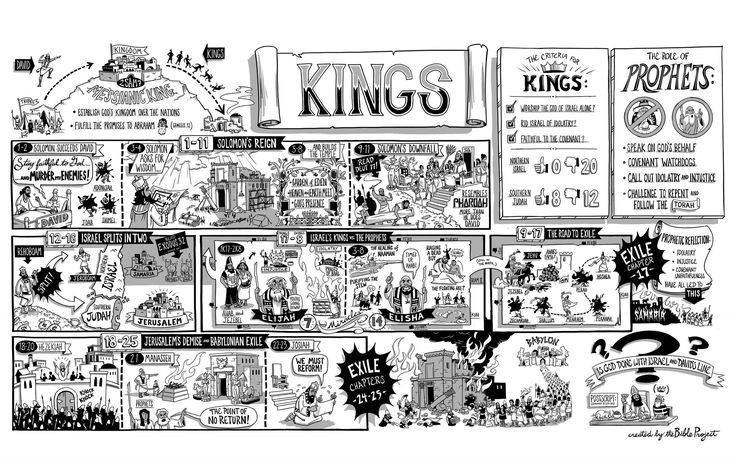
\includegraphics[scale=4, angle=90]{11OT-1Kings/References/BibleProject-1and2Kings}
\caption[1 and 2 Kings from the Bible Project]{1 and 2 Kings from the Bible Project}
\label{fig:1 and 2 Kings from the Bible Project}
\end{center}
\end{figure}

\newpage
\begin{figure}
\begin{center}
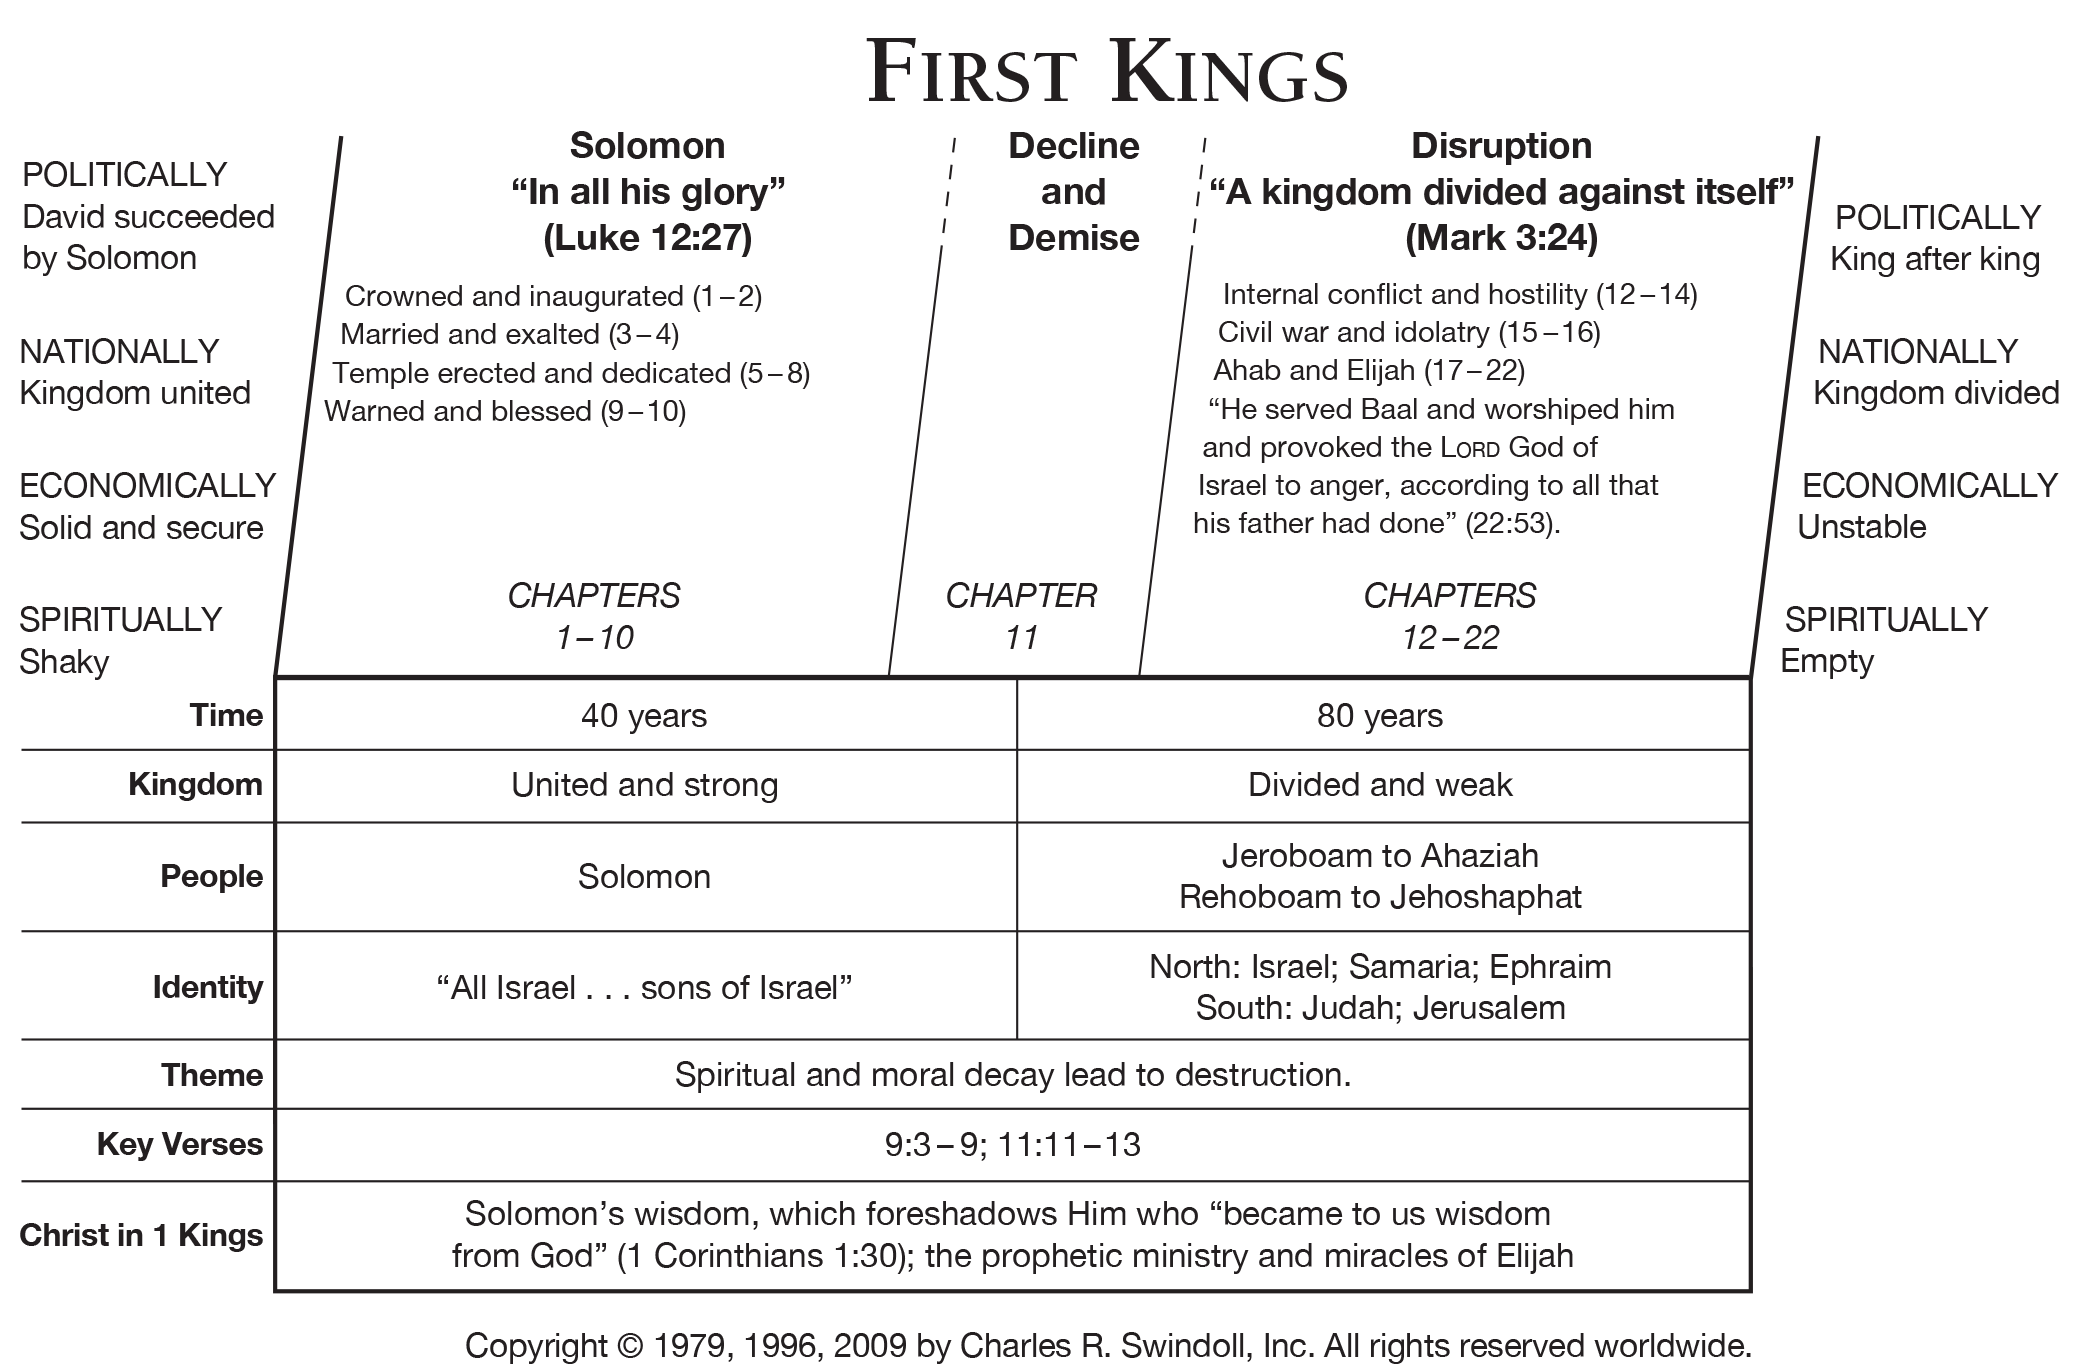
\includegraphics[scale=0.25, angle=90]{11OT-1Kings/References/Swindoll-1Kings}
\caption[1 Kings from Swindoll]{1 Kings from Swindoll}
\label{fig:1 Kings from Swindoll}
\end{center}
\end{figure}

\newpage
\begin{figure}
\begin{center}
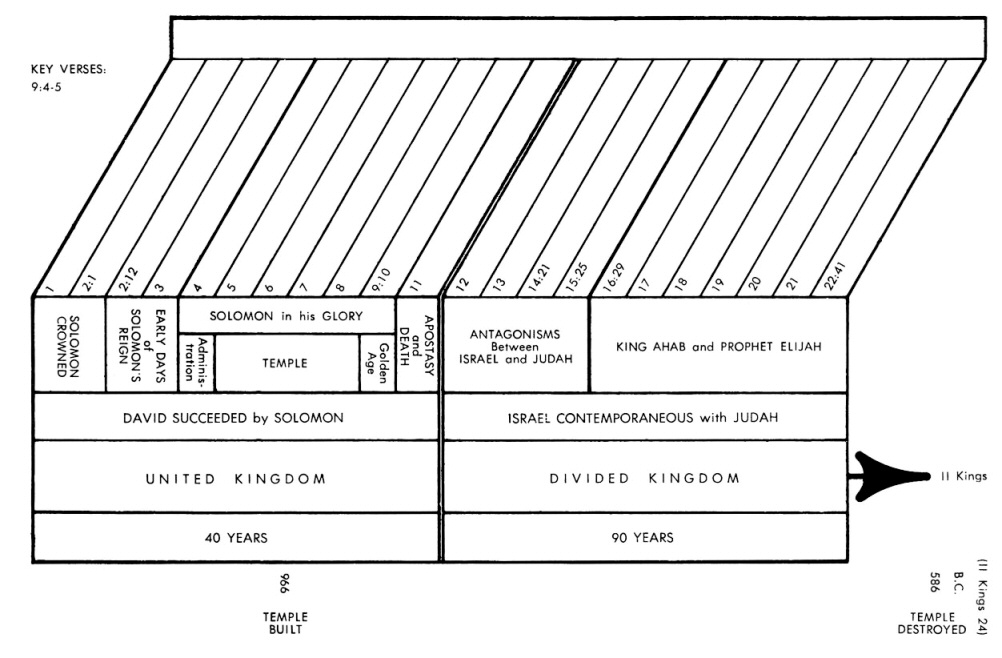
\includegraphics[scale=2, angle=90]{11OT-1Kings/References/Jensen1Kings}
\caption[1 Kings from Jensen]{1 Kings from Jensen}
\label{fig:1 Kings from Jensen}
\end{center}
\end{figure}

\newpage
\begin{figure}
\begin{center}
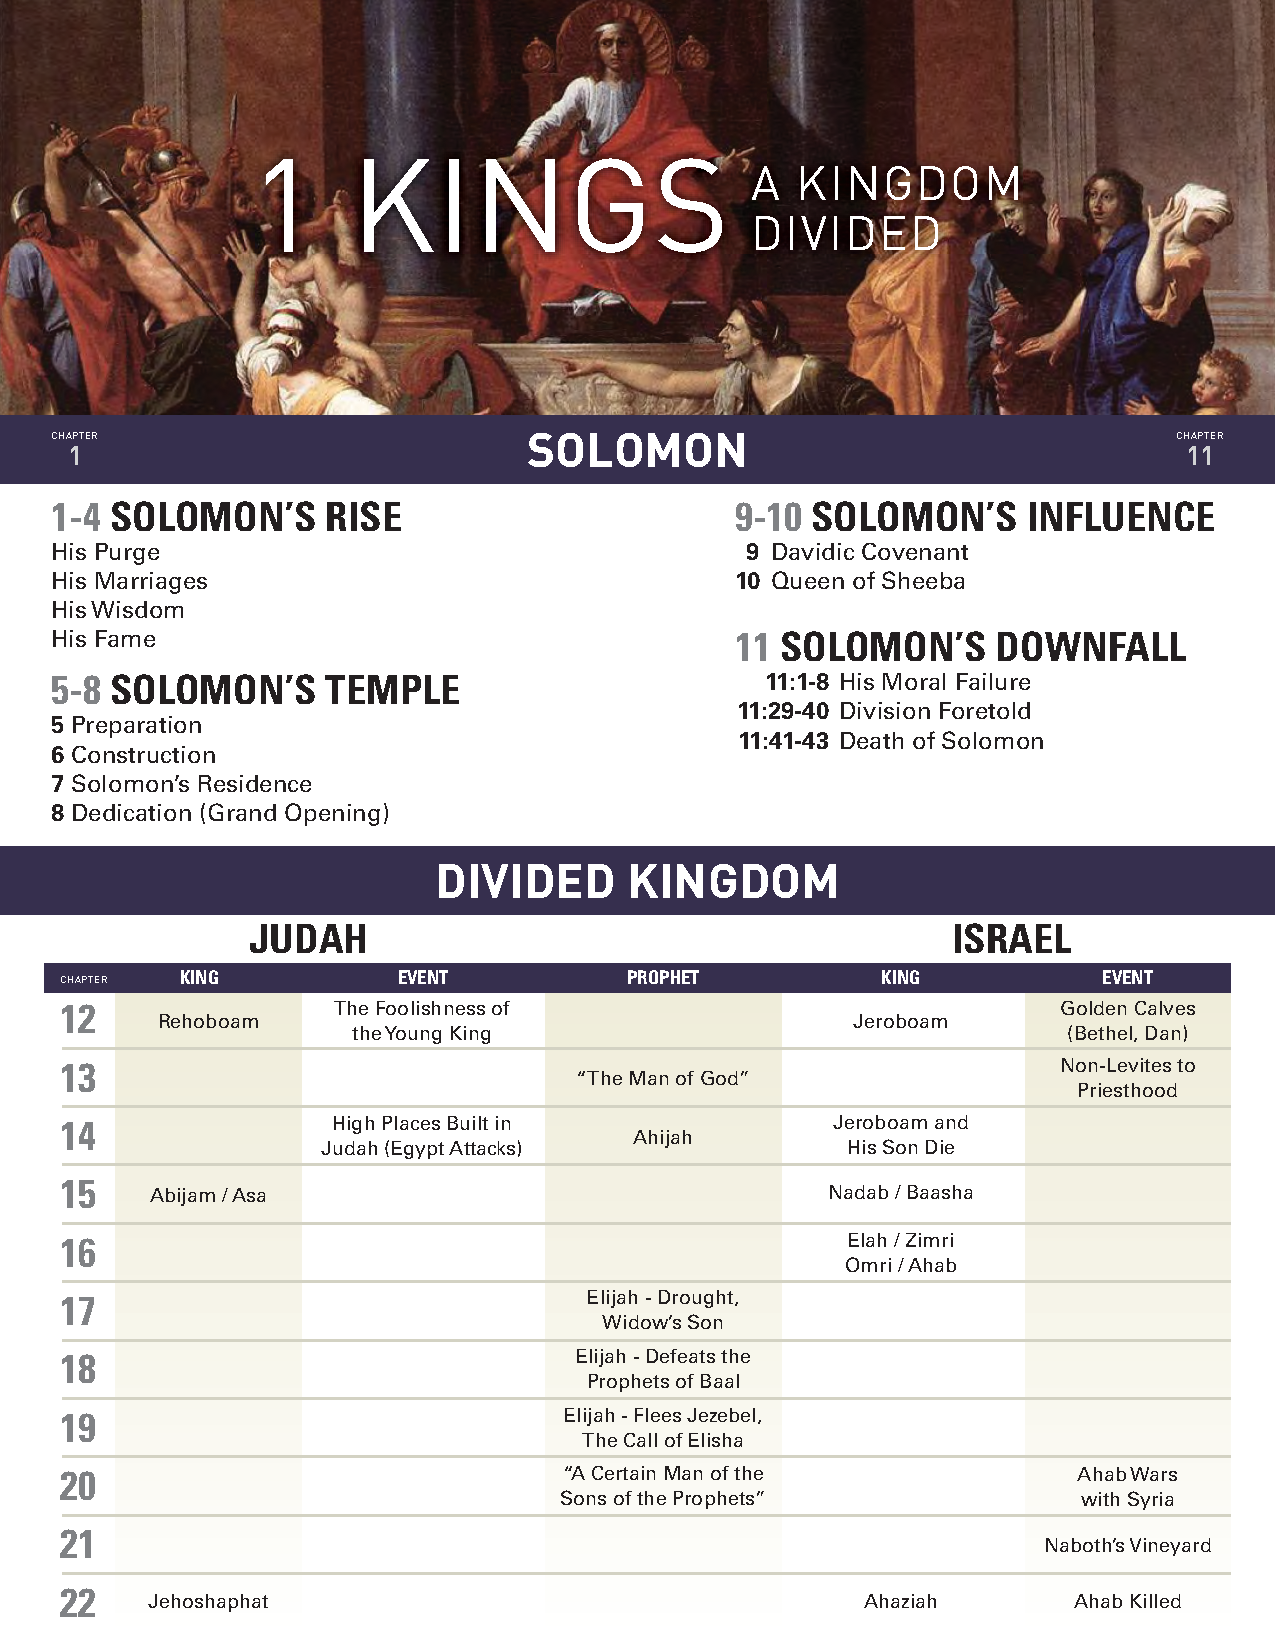
\includegraphics[scale=0.55, angle=0]{11OT-1Kings/References/1kings-chart}
\caption[1 Kings - the Divided Kingdom]{1 Kings - the Divided Kingdom}
\label{fig:1 Kings - the Divided Kingdom}
\end{center}
\end{figure}


\newpage
\begin{figure}
\begin{center}
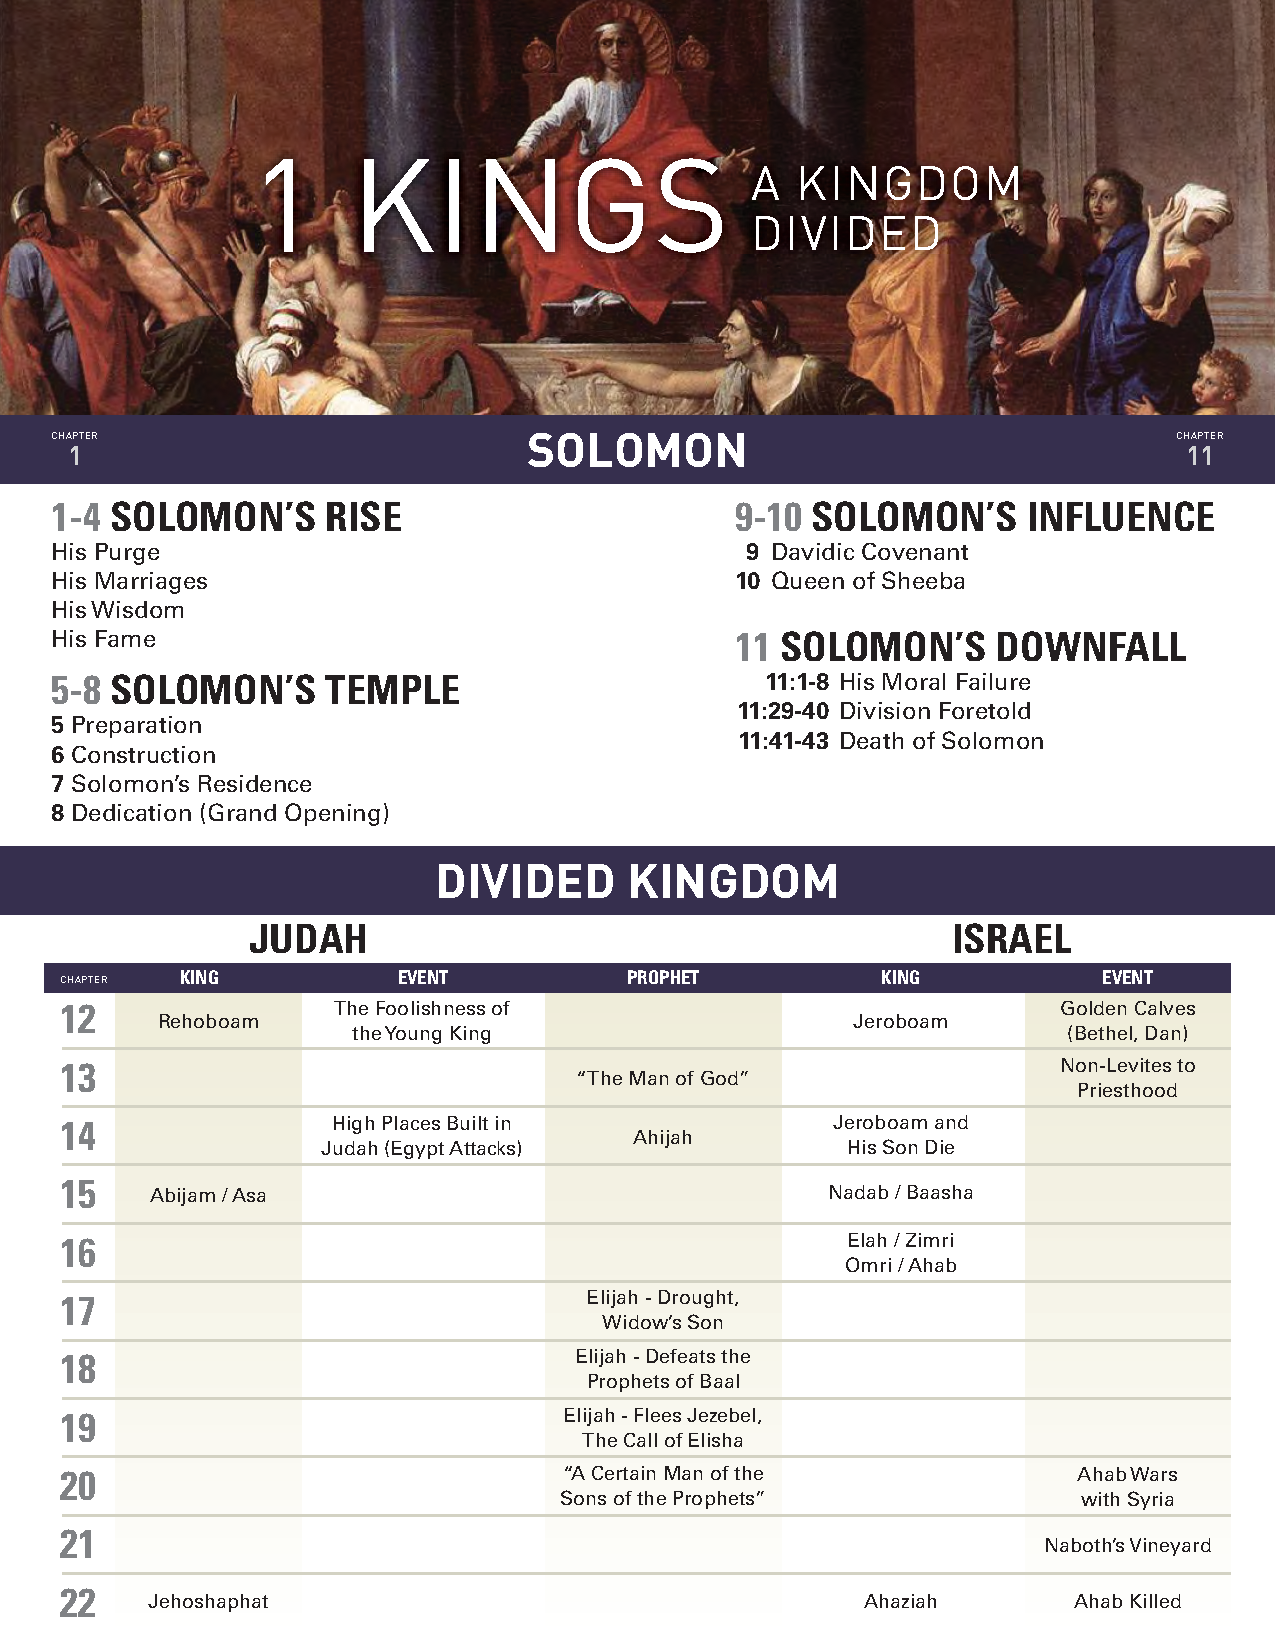
\includegraphics[scale=0.55, angle=0]{11OT-1Kings/References/1kings-chart}
\caption[1 Kings - the Divided Kingdom]{Walk-thru-the-Bible-chart-of-kings.pdf}
\label{fig:Chart of Kings from Walk Thru the Bible}
\end{center}
\end{figure}

\newpage
\begin{figure}
\begin{center}
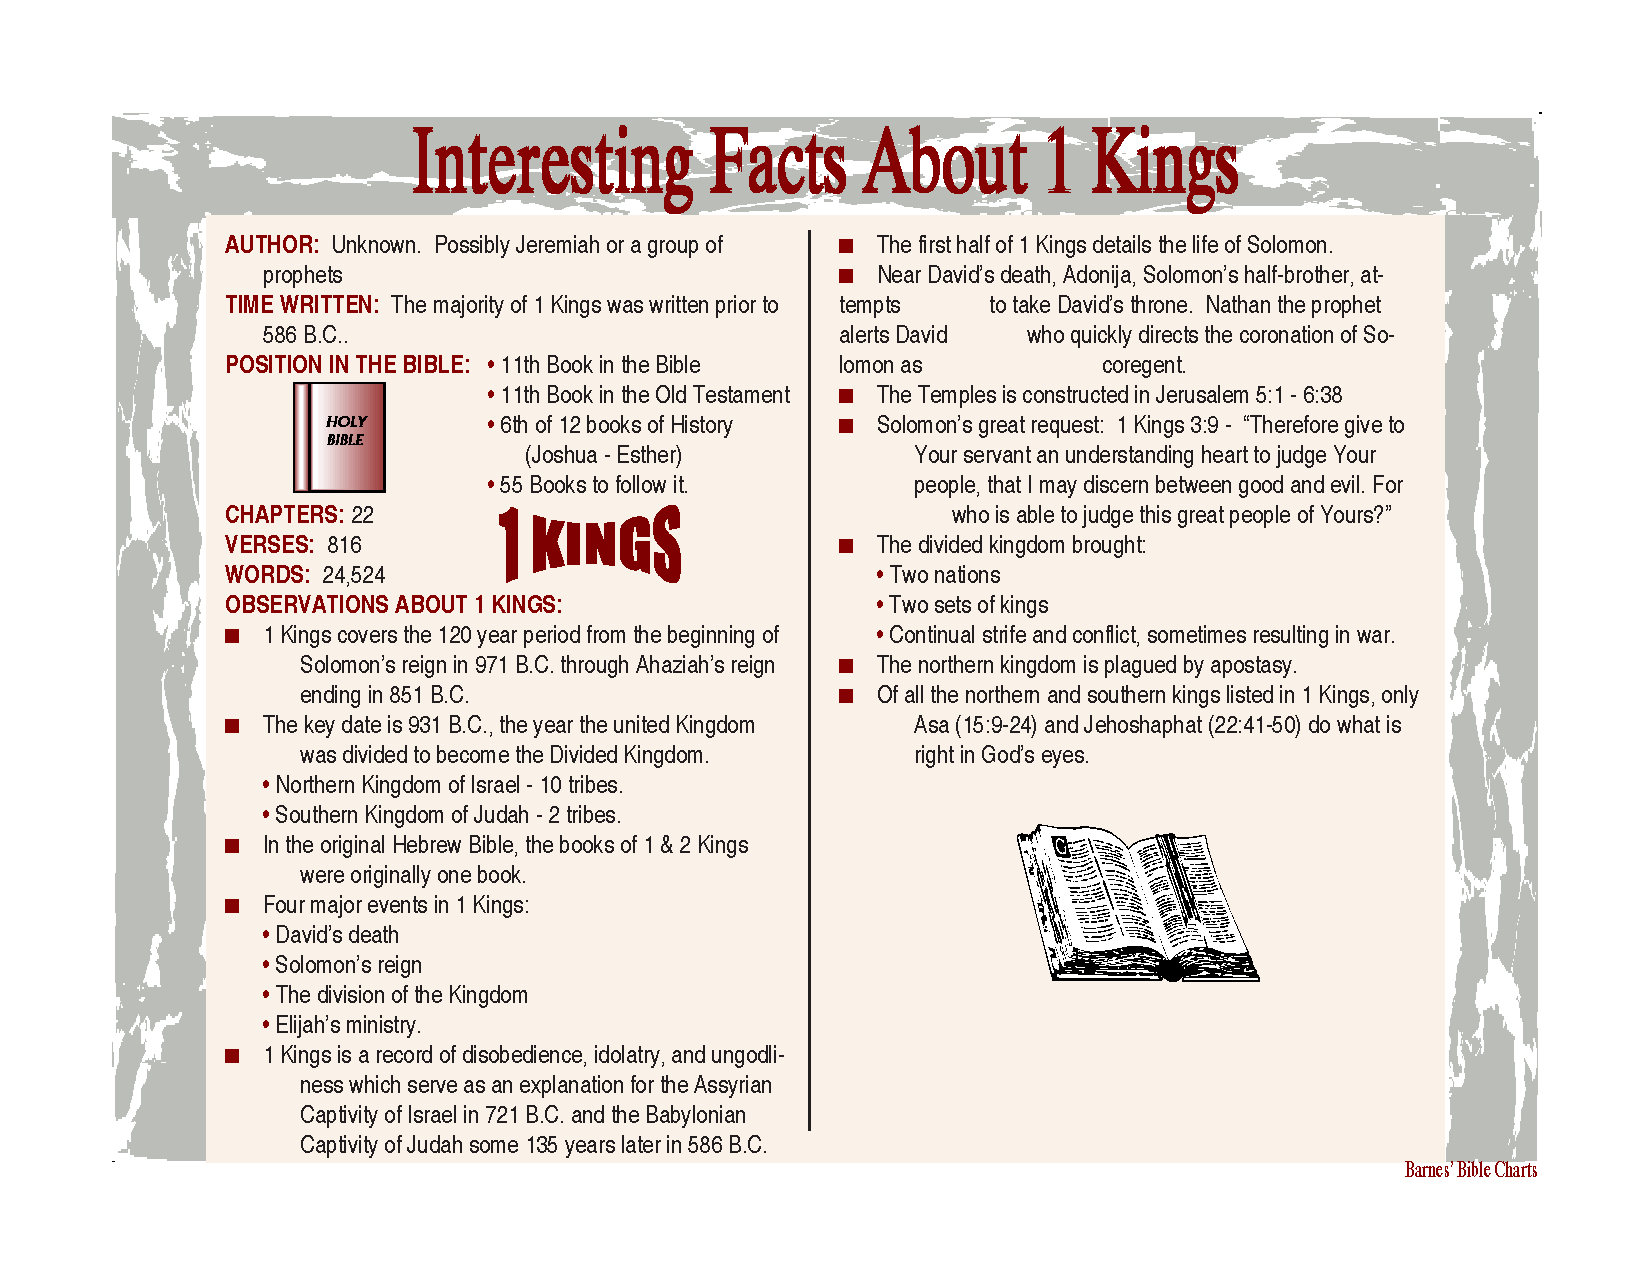
\includegraphics[scale=0.55, angle=90]{11OT-1Kings/References/interestingfactsaboutfirstkings.pdf}
\caption[1 Kings - the Divided Kingdom]{1 Kings - the Divided Kingdom}
\label{fig:1 Kings - the Divided Kingdom}
\end{center}
\end{figure}

\chapter{1 Kings 16}

\begin{figure}
  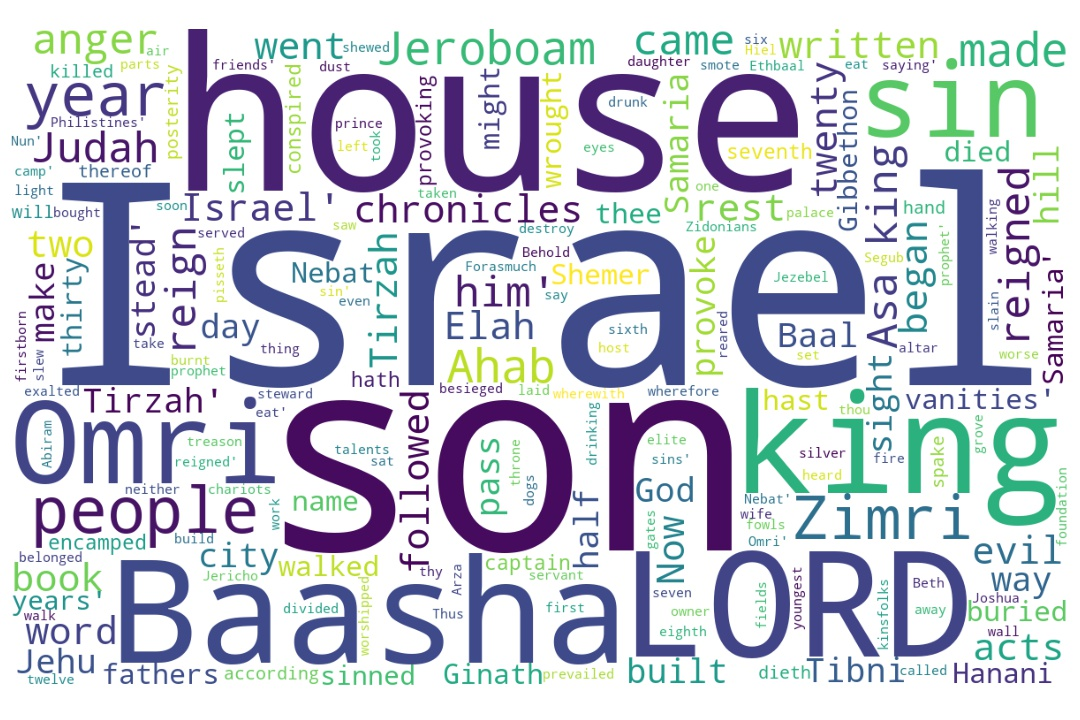
\includegraphics[width=\linewidth]{11OT-1Kings/1Kings16-WordCloud.jpg}
  \caption{1 Kings 16 Word Cloud}
  \label{fig:1 Kings 16 Word Cloud}
\end{figure}

%%%%%%%%%%%%%%%%%%%%%%%%%%%%%%%%%%%%%%%%%
%%%%%%%%%%%%%%%%%%%%%%%%%%%%%%%%%%%%%%%%%

\marginpar{\scriptsize \centering \fcolorbox{bone}{lime}{\textbf{JUST LIKE HEATHEN KINGS}}\\ (1 Kings 16) \begin{compactenum}[I.][8]
     \item The \textbf{Pedigree} \index[scripture]{1Kings!1Ki 16:02} (1Ki 16:2) 
    \item The \textbf{Prince} \index[scripture]{1Kings!1Ki 16:02} (1Ki 16:2) 
    \item The \textbf{Posterity} \index[scripture]{1Kings!1Ki 16:03} (1Ki 16:3) 
    \item The \textbf{Provocations} \index[scripture]{1Kings!1Ki 16:03} \index[scripture]{1Kings!1Ki 16:07}\index[scripture]{1Kings!1Ki 16:77} (1Ki 16:3, 7, 33) 
    \item A \textbf{Pattern} \index[scripture]{1Kings!1Ki 16:07} (1Kis 16:7) 
    \item The \textbf{Purge} \index[scripture]{1Kings!1Ki 16:11} (1Ki 16:11) 
    \item The \textbf{Palace} \index[scripture]{1Kings!1Ki 16:18} (1Ki 16:18) 
    \item The \textbf{Parts} \index[scripture]{1Kings!1Ki 16:21} (1Ki 16:21) 
\end{compactenum}}


\footnote{\textcolor[cmyk]{0.99998,1,0,0}{\hyperlink{TOC}{Return to end of Table of Contents.}}}\footnote{\href{https://audiobible.com/bible/1_kings_16.html}{\textcolor[cmyk]{0.99998,1,0,0}{1 Kings 16 Audio}}}\textcolor[cmyk]{0.99998,1,0,0}{Then the word of the LORD came to Jehu the son of Hanani against Baasha, saying,}
[2] \textcolor[cmyk]{0.99998,1,0,0}{Forasmuch as I exalted thee out of the dust, and made thee prince over my people Israel; and thou hast walked in the way of Jeroboam, and hast made my people Israel to sin, to provoke me to anger with their sins;}
[3] \textcolor[cmyk]{0.99998,1,0,0}{Behold, I will take away the posterity of Baasha, and the posterity of his house; and will make thy house like the house of Jeroboam the son of Nebat.}
[4] \textcolor[cmyk]{0.99998,1,0,0}{Him that dieth of Baasha in the city shall the dogs eat; and him that dieth of his in the fields shall the fowls of the air eat.}
[5] \textcolor[cmyk]{0.99998,1,0,0}{Now the rest of the acts of Baasha, and what he did, and his might, \emph{are} they not written in the book of the chronicles of the kings of Israel?}
[6] \textcolor[cmyk]{0.99998,1,0,0}{So Baasha slept with his fathers, and was buried in Tirzah: and Elah his son reigned in his stead.}
[7] \textcolor[cmyk]{0.99998,1,0,0}{And also by the hand of the prophet Jehu the son of Hanani came the word of the LORD against Baasha, and against his house, even for all the evil that he did in the sight of the LORD, in provoking him to anger with the work of his hands, in being like the house of Jeroboam; and because he killed him.}\\
\\
\P \textcolor[cmyk]{0.99998,1,0,0}{In the twenty and sixth year of Asa king of Judah began Elah the son of Baasha to reign over Israel in Tirzah, two years.}
[9] \textcolor[cmyk]{0.99998,1,0,0}{And his servant Zimri, captain of half \emph{his} chariots, conspired against him, as he was in Tirzah, drinking himself drunk in the house of Arza steward of \emph{his} house in Tirzah.}
[10] \textcolor[cmyk]{0.99998,1,0,0}{And Zimri went in and smote him, and killed him, in the twenty and seventh year of Asa king of Judah, and reigned in his stead.}\\
\\
\P \textcolor[cmyk]{0.99998,1,0,0}{And it came to pass, when he began to reign, as soon as he sat on his throne, \emph{that} he slew all the house of Baasha: he left him not one that pisseth against a wall, neither of his kinsfolks, nor of his friends.}
[12] \textcolor[cmyk]{0.99998,1,0,0}{Thus did Zimri destroy all the house of Baasha, according to the word of the LORD, which he spake against Baasha by Jehu the prophet,}
[13] \textcolor[cmyk]{0.99998,1,0,0}{For all the sins of Baasha, and the sins of Elah his son, by which they sinned, and by which they made Israel to sin, in provoking the LORD God of Israel to anger with their vanities.}
[14] \textcolor[cmyk]{0.99998,1,0,0}{Now the rest of the acts of Elah, and all that he did, \emph{are} they not written in the book of the chronicles of the kings of Israel?}\\\
\\
\P \textcolor[cmyk]{0.99998,1,0,0}{In the twenty and seventh year of Asa king of Judah did Zimri reign seven days in Tirzah. And the people \emph{were} encamped against Gibbethon, which \emph{belonged} to the Philistines.}
[16] \textcolor[cmyk]{0.99998,1,0,0}{And the people \emph{that} \emph{were} encamped heard say, Zimri hath conspired, and hath also slain the king: wherefore all Israel made Omri, the captain of the host, king over Israel that day in the camp.}
[17] \textcolor[cmyk]{0.99998,1,0,0}{And Omri went up from Gibbethon, and all Israel with him, and they besieged Tirzah.}
[18] \textcolor[cmyk]{0.99998,1,0,0}{And it came to pass, when Zimri saw that the city was taken, that he went into the palace of the king's house, and burnt the king's house over him with fire, and died,}
[19] \textcolor[cmyk]{0.99998,1,0,0}{For his sins which he sinned in doing evil in the sight of the LORD, in walking in the way of Jeroboam, and in his sin which he did, to make Israel to sin.}
[20] \textcolor[cmyk]{0.99998,1,0,0}{Now the rest of the acts of Zimri, and his treason that he wrought, \emph{are} they not written in the book of the chronicles of the kings of Israel?}\\
\\
\P \textcolor[cmyk]{0.99998,1,0,0}{Then were the people of Israel divided into two parts: half of the people followed Tibni the son of Ginath, to make him king; and half followed Omri.}
[22] \textcolor[cmyk]{0.99998,1,0,0}{But the people that followed Omri prevailed against the people that followed Tibni the son of Ginath: so Tibni died, and Omri reigned.}\\
\\
\P \textcolor[cmyk]{0.99998,1,0,0}{In the thirty and first year of Asa king of Judah began Omri to reign over Israel, twelve years: six years reigned he in Tirzah.}
[24] \textcolor[cmyk]{0.99998,1,0,0}{And he bought the hill Samaria of Shemer for two talents of silver, and built on the hill, and called the name of the city which he built, after the name of Shemer, owner of the hill, Samaria.}\\
\\
\P \textcolor[cmyk]{0.99998,1,0,0}{But Omri wrought evil in the eyes of the LORD, and did worse than all that \emph{were} before him.}
[26] \textcolor[cmyk]{0.99998,1,0,0}{For he walked in all the way of Jeroboam the son of Nebat, and in his sin wherewith he made Israel to sin, to provoke the LORD God of Israel to anger with their vanities.}
[27] \textcolor[cmyk]{0.99998,1,0,0}{Now the rest of the acts of Omri which he did, and his might that he shewed, \emph{are} they not written in the book of the chronicles of the kings of Israel?}
[28] \textcolor[cmyk]{0.99998,1,0,0}{So Omri slept with his fathers, and was buried in Samaria: and Ahab his son reigned in his stead.}\\
\\
\P \textcolor[cmyk]{0.99998,1,0,0}{And in the thirty and eighth year of Asa king of Judah began Ahab the son of Omri to reign over Israel: and Ahab the son of Omri reigned over Israel in Samaria twenty and two years.}
[30] \textcolor[cmyk]{0.99998,1,0,0}{And Ahab the son of Omri did evil in the sight of the LORD above all that \emph{were} before him.}
[31] \textcolor[cmyk]{0.99998,1,0,0}{And it came to pass, as if it had been a light thing for him to walk in the sins of Jeroboam the son of Nebat, that he took to wife Jezebel the daughter of Ethbaal king of the Zidonians, and went and served Baal, and worshipped him.}
[32] \textcolor[cmyk]{0.99998,1,0,0}{And he reared up an altar for Baal in the house of Baal, which he had built in Samaria.}
[33] \textcolor[cmyk]{0.99998,1,0,0}{And Ahab made a grove; and Ahab did more to provoke the LORD God of Israel to anger than all the kings of Israel that were before him.}\\
\\
\P \textcolor[cmyk]{0.99998,1,0,0}{In his days did Hiel the Beth-elite build Jericho: he laid the foundation thereof in Abiram his firstborn, and set up the gates thereof in his youngest \emph{son} Segub, according to the word of the LORD, which he spake by Joshua the son of Nun.}

\index[NWIV]{16!1Kings!1Ki 16:1}\index[AWIP]{Then!1Kings!1Ki 16:1}\index[AWIP]{the!1Kings!1Ki 16:1}\index[AWIP]{the!1Kings!1Ki 16:1 (2)}\index[AWIP]{the!1Kings!1Ki 16:1 (3)}\index[AWIP]{word!1Kings!1Ki 16:1}\index[AWIP]{of!1Kings!1Ki 16:1}\index[AWIP]{of!1Kings!1Ki 16:1 (2)}\index[AWIP]{LORD!1Kings!1Ki 16:1}\index[AWIP]{came!1Kings!1Ki 16:1}\index[AWIP]{to!1Kings!1Ki 16:1}\index[AWIP]{Jehu!1Kings!1Ki 16:1}\index[AWIP]{son!1Kings!1Ki 16:1}\index[AWIP]{Hanani!1Kings!1Ki 16:1}\index[AWIP]{against!1Kings!1Ki 16:1}\index[AWIP]{Baasha!1Kings!1Ki 16:1}\index[AWIP]{saying!1Kings!1Ki 16:1}

\index[NWIV]{42!1Kings!1Ki 16:2}\index[AWIP]{Forasmuch!1Kings!1Ki 16:2}\index[AWIP]{as!1Kings!1Ki 16:2}\index[AWIP]{I!1Kings!1Ki 16:2}\index[AWIP]{exalted!1Kings!1Ki 16:2}\index[AWIP]{thee!1Kings!1Ki 16:2}\index[AWIP]{thee!1Kings!1Ki 16:2 (2)}\index[AWIP]{out!1Kings!1Ki 16:2}\index[AWIP]{of!1Kings!1Ki 16:2}\index[AWIP]{of!1Kings!1Ki 16:2 (2)}\index[AWIP]{the!1Kings!1Ki 16:2}\index[AWIP]{the!1Kings!1Ki 16:2 (2)}\index[AWIP]{dust!1Kings!1Ki 16:2}\index[AWIP]{and!1Kings!1Ki 16:2}\index[AWIP]{and!1Kings!1Ki 16:2 (2)}\index[AWIP]{and!1Kings!1Ki 16:2 (3)}\index[AWIP]{made!1Kings!1Ki 16:2}\index[AWIP]{made!1Kings!1Ki 16:2 (2)}\index[AWIP]{prince!1Kings!1Ki 16:2}\index[AWIP]{over!1Kings!1Ki 16:2}\index[AWIP]{my!1Kings!1Ki 16:2}\index[AWIP]{my!1Kings!1Ki 16:2 (2)}\index[AWIP]{people!1Kings!1Ki 16:2}\index[AWIP]{people!1Kings!1Ki 16:2 (2)}\index[AWIP]{Israel!1Kings!1Ki 16:2}\index[AWIP]{Israel!1Kings!1Ki 16:2 (2)}\index[AWIP]{thou!1Kings!1Ki 16:2}\index[AWIP]{hast!1Kings!1Ki 16:2}\index[AWIP]{hast!1Kings!1Ki 16:2 (2)}\index[AWIP]{walked!1Kings!1Ki 16:2}\index[AWIP]{in!1Kings!1Ki 16:2}\index[AWIP]{way!1Kings!1Ki 16:2}\index[AWIP]{Jeroboam!1Kings!1Ki 16:2}\index[AWIP]{to!1Kings!1Ki 16:2}\index[AWIP]{to!1Kings!1Ki 16:2 (2)}\index[AWIP]{to!1Kings!1Ki 16:2 (3)}\index[AWIP]{sin!1Kings!1Ki 16:2}\index[AWIP]{provoke!1Kings!1Ki 16:2}\index[AWIP]{me!1Kings!1Ki 16:2}\index[AWIP]{anger!1Kings!1Ki 16:2}\index[AWIP]{with!1Kings!1Ki 16:2}\index[AWIP]{their!1Kings!1Ki 16:2}\index[AWIP]{sins!1Kings!1Ki 16:2}

\index[NWIV]{29!1Kings!1Ki 16:3}\index[AWIP]{Behold!1Kings!1Ki 16:3}\index[AWIP]{I!1Kings!1Ki 16:3}\index[AWIP]{will!1Kings!1Ki 16:3}\index[AWIP]{will!1Kings!1Ki 16:3 (2)}\index[AWIP]{take!1Kings!1Ki 16:3}\index[AWIP]{away!1Kings!1Ki 16:3}\index[AWIP]{the!1Kings!1Ki 16:3}\index[AWIP]{the!1Kings!1Ki 16:3 (2)}\index[AWIP]{the!1Kings!1Ki 16:3 (3)}\index[AWIP]{the!1Kings!1Ki 16:3 (4)}\index[AWIP]{posterity!1Kings!1Ki 16:3}\index[AWIP]{posterity!1Kings!1Ki 16:3 (2)}\index[AWIP]{of!1Kings!1Ki 16:3}\index[AWIP]{of!1Kings!1Ki 16:3 (2)}\index[AWIP]{of!1Kings!1Ki 16:3 (3)}\index[AWIP]{of!1Kings!1Ki 16:3 (4)}\index[AWIP]{Baasha!1Kings!1Ki 16:3}\index[AWIP]{and!1Kings!1Ki 16:3}\index[AWIP]{and!1Kings!1Ki 16:3 (2)}\index[AWIP]{his!1Kings!1Ki 16:3}\index[AWIP]{house!1Kings!1Ki 16:3}\index[AWIP]{house!1Kings!1Ki 16:3 (2)}\index[AWIP]{house!1Kings!1Ki 16:3 (3)}\index[AWIP]{make!1Kings!1Ki 16:3}\index[AWIP]{thy!1Kings!1Ki 16:3}\index[AWIP]{like!1Kings!1Ki 16:3}\index[AWIP]{Jeroboam!1Kings!1Ki 16:3}\index[AWIP]{son!1Kings!1Ki 16:3}\index[AWIP]{Nebat!1Kings!1Ki 16:3}

\index[NWIV]{28!1Kings!1Ki 16:4}\index[AWIP]{Him!1Kings!1Ki 16:4}\index[AWIP]{that!1Kings!1Ki 16:4}\index[AWIP]{that!1Kings!1Ki 16:4 (2)}\index[AWIP]{dieth!1Kings!1Ki 16:4}\index[AWIP]{dieth!1Kings!1Ki 16:4 (2)}\index[AWIP]{of!1Kings!1Ki 16:4}\index[AWIP]{of!1Kings!1Ki 16:4 (2)}\index[AWIP]{of!1Kings!1Ki 16:4 (3)}\index[AWIP]{Baasha!1Kings!1Ki 16:4}\index[AWIP]{in!1Kings!1Ki 16:4}\index[AWIP]{in!1Kings!1Ki 16:4 (2)}\index[AWIP]{the!1Kings!1Ki 16:4}\index[AWIP]{the!1Kings!1Ki 16:4 (2)}\index[AWIP]{the!1Kings!1Ki 16:4 (3)}\index[AWIP]{the!1Kings!1Ki 16:4 (4)}\index[AWIP]{the!1Kings!1Ki 16:4 (5)}\index[AWIP]{city!1Kings!1Ki 16:4}\index[AWIP]{shall!1Kings!1Ki 16:4}\index[AWIP]{shall!1Kings!1Ki 16:4 (2)}\index[AWIP]{dogs!1Kings!1Ki 16:4}\index[AWIP]{eat!1Kings!1Ki 16:4}\index[AWIP]{eat!1Kings!1Ki 16:4 (2)}\index[AWIP]{and!1Kings!1Ki 16:4}\index[AWIP]{him!1Kings!1Ki 16:4}\index[AWIP]{his!1Kings!1Ki 16:4}\index[AWIP]{fields!1Kings!1Ki 16:4}\index[AWIP]{fowls!1Kings!1Ki 16:4}\index[AWIP]{air!1Kings!1Ki 16:4}

\index[NWIV]{30!1Kings!1Ki 16:5}\index[AWIP]{Now!1Kings!1Ki 16:5}\index[AWIP]{the!1Kings!1Ki 16:5}\index[AWIP]{the!1Kings!1Ki 16:5 (2)}\index[AWIP]{the!1Kings!1Ki 16:5 (3)}\index[AWIP]{the!1Kings!1Ki 16:5 (4)}\index[AWIP]{the!1Kings!1Ki 16:5 (5)}\index[AWIP]{rest!1Kings!1Ki 16:5}\index[AWIP]{of!1Kings!1Ki 16:5}\index[AWIP]{of!1Kings!1Ki 16:5 (2)}\index[AWIP]{of!1Kings!1Ki 16:5 (3)}\index[AWIP]{of!1Kings!1Ki 16:5 (4)}\index[AWIP]{of!1Kings!1Ki 16:5 (5)}\index[AWIP]{acts!1Kings!1Ki 16:5}\index[AWIP]{Baasha!1Kings!1Ki 16:5}\index[AWIP]{and!1Kings!1Ki 16:5}\index[AWIP]{and!1Kings!1Ki 16:5 (2)}\index[AWIP]{what!1Kings!1Ki 16:5}\index[AWIP]{he!1Kings!1Ki 16:5}\index[AWIP]{did!1Kings!1Ki 16:5}\index[AWIP]{his!1Kings!1Ki 16:5}\index[AWIP]{might!1Kings!1Ki 16:5}\index[AWIP]{\emph{are}!1Kings!1Ki 16:5}\index[AWIP]{they!1Kings!1Ki 16:5}\index[AWIP]{not!1Kings!1Ki 16:5}\index[AWIP]{written!1Kings!1Ki 16:5}\index[AWIP]{in!1Kings!1Ki 16:5}\index[AWIP]{book!1Kings!1Ki 16:5}\index[AWIP]{chronicles!1Kings!1Ki 16:5}\index[AWIP]{kings!1Kings!1Ki 16:5}\index[AWIP]{Israel?!1Kings!1Ki 16:5}\index[AWIP]{\emph{are}!1Kings!1Ki 16:5}

\index[NWIV]{19!1Kings!1Ki 16:6}\index[AWIP]{So!1Kings!1Ki 16:6}\index[AWIP]{Baasha!1Kings!1Ki 16:6}\index[AWIP]{slept!1Kings!1Ki 16:6}\index[AWIP]{with!1Kings!1Ki 16:6}\index[AWIP]{his!1Kings!1Ki 16:6}\index[AWIP]{his!1Kings!1Ki 16:6 (2)}\index[AWIP]{his!1Kings!1Ki 16:6 (3)}\index[AWIP]{fathers!1Kings!1Ki 16:6}\index[AWIP]{and!1Kings!1Ki 16:6}\index[AWIP]{and!1Kings!1Ki 16:6 (2)}\index[AWIP]{was!1Kings!1Ki 16:6}\index[AWIP]{buried!1Kings!1Ki 16:6}\index[AWIP]{in!1Kings!1Ki 16:6}\index[AWIP]{in!1Kings!1Ki 16:6 (2)}\index[AWIP]{Tirzah!1Kings!1Ki 16:6}\index[AWIP]{Elah!1Kings!1Ki 16:6}\index[AWIP]{son!1Kings!1Ki 16:6}\index[AWIP]{reigned!1Kings!1Ki 16:6}\index[AWIP]{stead!1Kings!1Ki 16:6}

\index[NWIV]{62!1Kings!1Ki 16:7}\index[AWIP]{And!1Kings!1Ki 16:7}\index[AWIP]{also!1Kings!1Ki 16:7}\index[AWIP]{by!1Kings!1Ki 16:7}\index[AWIP]{the!1Kings!1Ki 16:7}\index[AWIP]{the!1Kings!1Ki 16:7 (2)}\index[AWIP]{the!1Kings!1Ki 16:7 (3)}\index[AWIP]{the!1Kings!1Ki 16:7 (4)}\index[AWIP]{the!1Kings!1Ki 16:7 (5)}\index[AWIP]{the!1Kings!1Ki 16:7 (6)}\index[AWIP]{the!1Kings!1Ki 16:7 (7)}\index[AWIP]{the!1Kings!1Ki 16:7 (8)}\index[AWIP]{the!1Kings!1Ki 16:7 (9)}\index[AWIP]{the!1Kings!1Ki 16:7 (10)}\index[AWIP]{hand!1Kings!1Ki 16:7}\index[AWIP]{of!1Kings!1Ki 16:7}\index[AWIP]{of!1Kings!1Ki 16:7 (2)}\index[AWIP]{of!1Kings!1Ki 16:7 (3)}\index[AWIP]{of!1Kings!1Ki 16:7 (4)}\index[AWIP]{of!1Kings!1Ki 16:7 (5)}\index[AWIP]{of!1Kings!1Ki 16:7 (6)}\index[AWIP]{prophet!1Kings!1Ki 16:7}\index[AWIP]{Jehu!1Kings!1Ki 16:7}\index[AWIP]{son!1Kings!1Ki 16:7}\index[AWIP]{Hanani!1Kings!1Ki 16:7}\index[AWIP]{came!1Kings!1Ki 16:7}\index[AWIP]{word!1Kings!1Ki 16:7}\index[AWIP]{LORD!1Kings!1Ki 16:7}\index[AWIP]{LORD!1Kings!1Ki 16:7 (2)}\index[AWIP]{against!1Kings!1Ki 16:7}\index[AWIP]{against!1Kings!1Ki 16:7 (2)}\index[AWIP]{Baasha!1Kings!1Ki 16:7}\index[AWIP]{and!1Kings!1Ki 16:7}\index[AWIP]{and!1Kings!1Ki 16:7 (2)}\index[AWIP]{his!1Kings!1Ki 16:7}\index[AWIP]{his!1Kings!1Ki 16:7 (2)}\index[AWIP]{house!1Kings!1Ki 16:7}\index[AWIP]{house!1Kings!1Ki 16:7 (2)}\index[AWIP]{even!1Kings!1Ki 16:7}\index[AWIP]{for!1Kings!1Ki 16:7}\index[AWIP]{all!1Kings!1Ki 16:7}\index[AWIP]{evil!1Kings!1Ki 16:7}\index[AWIP]{that!1Kings!1Ki 16:7}\index[AWIP]{he!1Kings!1Ki 16:7}\index[AWIP]{he!1Kings!1Ki 16:7 (2)}\index[AWIP]{did!1Kings!1Ki 16:7}\index[AWIP]{in!1Kings!1Ki 16:7}\index[AWIP]{in!1Kings!1Ki 16:7 (2)}\index[AWIP]{in!1Kings!1Ki 16:7 (3)}\index[AWIP]{sight!1Kings!1Ki 16:7}\index[AWIP]{provoking!1Kings!1Ki 16:7}\index[AWIP]{him!1Kings!1Ki 16:7}\index[AWIP]{him!1Kings!1Ki 16:7 (2)}\index[AWIP]{to!1Kings!1Ki 16:7}\index[AWIP]{anger!1Kings!1Ki 16:7}\index[AWIP]{with!1Kings!1Ki 16:7}\index[AWIP]{work!1Kings!1Ki 16:7}\index[AWIP]{hands!1Kings!1Ki 16:7}\index[AWIP]{being!1Kings!1Ki 16:7}\index[AWIP]{like!1Kings!1Ki 16:7}\index[AWIP]{Jeroboam!1Kings!1Ki 16:7}\index[AWIP]{because!1Kings!1Ki 16:7}\index[AWIP]{killed!1Kings!1Ki 16:7}

\index[NWIV]{25!1Kings!1Ki 16:8}\index[AWIP]{In!1Kings!1Ki 16:8}\index[AWIP]{the!1Kings!1Ki 16:8}\index[AWIP]{the!1Kings!1Ki 16:8 (2)}\index[AWIP]{twenty!1Kings!1Ki 16:8}\index[AWIP]{and!1Kings!1Ki 16:8}\index[AWIP]{sixth!1Kings!1Ki 16:8}\index[AWIP]{year!1Kings!1Ki 16:8}\index[AWIP]{of!1Kings!1Ki 16:8}\index[AWIP]{of!1Kings!1Ki 16:8 (2)}\index[AWIP]{of!1Kings!1Ki 16:8 (3)}\index[AWIP]{Asa!1Kings!1Ki 16:8}\index[AWIP]{king!1Kings!1Ki 16:8}\index[AWIP]{Judah!1Kings!1Ki 16:8}\index[AWIP]{began!1Kings!1Ki 16:8}\index[AWIP]{Elah!1Kings!1Ki 16:8}\index[AWIP]{son!1Kings!1Ki 16:8}\index[AWIP]{Baasha!1Kings!1Ki 16:8}\index[AWIP]{to!1Kings!1Ki 16:8}\index[AWIP]{reign!1Kings!1Ki 16:8}\index[AWIP]{over!1Kings!1Ki 16:8}\index[AWIP]{Israel!1Kings!1Ki 16:8}\index[AWIP]{in!1Kings!1Ki 16:8}\index[AWIP]{Tirzah!1Kings!1Ki 16:8}\index[AWIP]{two!1Kings!1Ki 16:8}\index[AWIP]{years!1Kings!1Ki 16:8}

\index[NWIV]{31!1Kings!1Ki 16:9}\index[AWIP]{And!1Kings!1Ki 16:9}\index[AWIP]{his!1Kings!1Ki 16:9}\index[AWIP]{servant!1Kings!1Ki 16:9}\index[AWIP]{Zimri!1Kings!1Ki 16:9}\index[AWIP]{captain!1Kings!1Ki 16:9}\index[AWIP]{of!1Kings!1Ki 16:9}\index[AWIP]{of!1Kings!1Ki 16:9 (2)}\index[AWIP]{of!1Kings!1Ki 16:9 (3)}\index[AWIP]{half!1Kings!1Ki 16:9}\index[AWIP]{\emph{his}!1Kings!1Ki 16:9}\index[AWIP]{\emph{his}!1Kings!1Ki 16:9 (2)}\index[AWIP]{chariots!1Kings!1Ki 16:9}\index[AWIP]{conspired!1Kings!1Ki 16:9}\index[AWIP]{against!1Kings!1Ki 16:9}\index[AWIP]{him!1Kings!1Ki 16:9}\index[AWIP]{as!1Kings!1Ki 16:9}\index[AWIP]{he!1Kings!1Ki 16:9}\index[AWIP]{was!1Kings!1Ki 16:9}\index[AWIP]{in!1Kings!1Ki 16:9}\index[AWIP]{in!1Kings!1Ki 16:9 (2)}\index[AWIP]{in!1Kings!1Ki 16:9 (3)}\index[AWIP]{Tirzah!1Kings!1Ki 16:9}\index[AWIP]{Tirzah!1Kings!1Ki 16:9 (2)}\index[AWIP]{drinking!1Kings!1Ki 16:9}\index[AWIP]{himself!1Kings!1Ki 16:9}\index[AWIP]{drunk!1Kings!1Ki 16:9}\index[AWIP]{the!1Kings!1Ki 16:9}\index[AWIP]{house!1Kings!1Ki 16:9}\index[AWIP]{house!1Kings!1Ki 16:9 (2)}\index[AWIP]{Arza!1Kings!1Ki 16:9}\index[AWIP]{steward!1Kings!1Ki 16:9}\index[AWIP]{\emph{his}!1Kings!1Ki 16:9}\index[AWIP]{\emph{his}!1Kings!1Ki 16:9 (2)}

\index[NWIV]{26!1Kings!1Ki 16:10}\index[AWIP]{And!1Kings!1Ki 16:10}\index[AWIP]{Zimri!1Kings!1Ki 16:10}\index[AWIP]{went!1Kings!1Ki 16:10}\index[AWIP]{in!1Kings!1Ki 16:10}\index[AWIP]{in!1Kings!1Ki 16:10 (2)}\index[AWIP]{in!1Kings!1Ki 16:10 (3)}\index[AWIP]{and!1Kings!1Ki 16:10}\index[AWIP]{and!1Kings!1Ki 16:10 (2)}\index[AWIP]{and!1Kings!1Ki 16:10 (3)}\index[AWIP]{and!1Kings!1Ki 16:10 (4)}\index[AWIP]{smote!1Kings!1Ki 16:10}\index[AWIP]{him!1Kings!1Ki 16:10}\index[AWIP]{him!1Kings!1Ki 16:10 (2)}\index[AWIP]{killed!1Kings!1Ki 16:10}\index[AWIP]{the!1Kings!1Ki 16:10}\index[AWIP]{twenty!1Kings!1Ki 16:10}\index[AWIP]{seventh!1Kings!1Ki 16:10}\index[AWIP]{year!1Kings!1Ki 16:10}\index[AWIP]{of!1Kings!1Ki 16:10}\index[AWIP]{of!1Kings!1Ki 16:10 (2)}\index[AWIP]{Asa!1Kings!1Ki 16:10}\index[AWIP]{king!1Kings!1Ki 16:10}\index[AWIP]{Judah!1Kings!1Ki 16:10}\index[AWIP]{reigned!1Kings!1Ki 16:10}\index[AWIP]{his!1Kings!1Ki 16:10}\index[AWIP]{stead!1Kings!1Ki 16:10}

\index[NWIV]{44!1Kings!1Ki 16:11}\index[AWIP]{And!1Kings!1Ki 16:11}\index[AWIP]{it!1Kings!1Ki 16:11}\index[AWIP]{came!1Kings!1Ki 16:11}\index[AWIP]{to!1Kings!1Ki 16:11}\index[AWIP]{to!1Kings!1Ki 16:11 (2)}\index[AWIP]{pass!1Kings!1Ki 16:11}\index[AWIP]{when!1Kings!1Ki 16:11}\index[AWIP]{he!1Kings!1Ki 16:11}\index[AWIP]{he!1Kings!1Ki 16:11 (2)}\index[AWIP]{he!1Kings!1Ki 16:11 (3)}\index[AWIP]{he!1Kings!1Ki 16:11 (4)}\index[AWIP]{began!1Kings!1Ki 16:11}\index[AWIP]{reign!1Kings!1Ki 16:11}\index[AWIP]{as!1Kings!1Ki 16:11}\index[AWIP]{as!1Kings!1Ki 16:11 (2)}\index[AWIP]{soon!1Kings!1Ki 16:11}\index[AWIP]{sat!1Kings!1Ki 16:11}\index[AWIP]{on!1Kings!1Ki 16:11}\index[AWIP]{his!1Kings!1Ki 16:11}\index[AWIP]{his!1Kings!1Ki 16:11 (2)}\index[AWIP]{his!1Kings!1Ki 16:11 (3)}\index[AWIP]{throne!1Kings!1Ki 16:11}\index[AWIP]{\emph{that}!1Kings!1Ki 16:11}\index[AWIP]{slew!1Kings!1Ki 16:11}\index[AWIP]{all!1Kings!1Ki 16:11}\index[AWIP]{the!1Kings!1Ki 16:11}\index[AWIP]{house!1Kings!1Ki 16:11}\index[AWIP]{of!1Kings!1Ki 16:11}\index[AWIP]{of!1Kings!1Ki 16:11 (2)}\index[AWIP]{of!1Kings!1Ki 16:11 (3)}\index[AWIP]{Baasha!1Kings!1Ki 16:11}\index[AWIP]{left!1Kings!1Ki 16:11}\index[AWIP]{him!1Kings!1Ki 16:11}\index[AWIP]{not!1Kings!1Ki 16:11}\index[AWIP]{one!1Kings!1Ki 16:11}\index[AWIP]{that!1Kings!1Ki 16:11}\index[AWIP]{pisseth!1Kings!1Ki 16:11}\index[AWIP]{against!1Kings!1Ki 16:11}\index[AWIP]{a!1Kings!1Ki 16:11}\index[AWIP]{wall!1Kings!1Ki 16:11}\index[AWIP]{neither!1Kings!1Ki 16:11}\index[AWIP]{kinsfolks!1Kings!1Ki 16:11}\index[AWIP]{nor!1Kings!1Ki 16:11}\index[AWIP]{friends!1Kings!1Ki 16:11}\index[AWIP]{\emph{that}!1Kings!1Ki 16:11}

\index[NWIV]{25!1Kings!1Ki 16:12}\index[AWIP]{Thus!1Kings!1Ki 16:12}\index[AWIP]{did!1Kings!1Ki 16:12}\index[AWIP]{Zimri!1Kings!1Ki 16:12}\index[AWIP]{destroy!1Kings!1Ki 16:12}\index[AWIP]{all!1Kings!1Ki 16:12}\index[AWIP]{the!1Kings!1Ki 16:12}\index[AWIP]{the!1Kings!1Ki 16:12 (2)}\index[AWIP]{the!1Kings!1Ki 16:12 (3)}\index[AWIP]{the!1Kings!1Ki 16:12 (4)}\index[AWIP]{house!1Kings!1Ki 16:12}\index[AWIP]{of!1Kings!1Ki 16:12}\index[AWIP]{of!1Kings!1Ki 16:12 (2)}\index[AWIP]{Baasha!1Kings!1Ki 16:12}\index[AWIP]{Baasha!1Kings!1Ki 16:12 (2)}\index[AWIP]{according!1Kings!1Ki 16:12}\index[AWIP]{to!1Kings!1Ki 16:12}\index[AWIP]{word!1Kings!1Ki 16:12}\index[AWIP]{LORD!1Kings!1Ki 16:12}\index[AWIP]{which!1Kings!1Ki 16:12}\index[AWIP]{he!1Kings!1Ki 16:12}\index[AWIP]{spake!1Kings!1Ki 16:12}\index[AWIP]{against!1Kings!1Ki 16:12}\index[AWIP]{by!1Kings!1Ki 16:12}\index[AWIP]{Jehu!1Kings!1Ki 16:12}\index[AWIP]{prophet!1Kings!1Ki 16:12}

\index[NWIV]{37!1Kings!1Ki 16:13}\index[AWIP]{For!1Kings!1Ki 16:13}\index[AWIP]{all!1Kings!1Ki 16:13}\index[AWIP]{the!1Kings!1Ki 16:13}\index[AWIP]{the!1Kings!1Ki 16:13 (2)}\index[AWIP]{the!1Kings!1Ki 16:13 (3)}\index[AWIP]{sins!1Kings!1Ki 16:13}\index[AWIP]{sins!1Kings!1Ki 16:13 (2)}\index[AWIP]{of!1Kings!1Ki 16:13}\index[AWIP]{of!1Kings!1Ki 16:13 (2)}\index[AWIP]{of!1Kings!1Ki 16:13 (3)}\index[AWIP]{Baasha!1Kings!1Ki 16:13}\index[AWIP]{and!1Kings!1Ki 16:13}\index[AWIP]{and!1Kings!1Ki 16:13 (2)}\index[AWIP]{Elah!1Kings!1Ki 16:13}\index[AWIP]{his!1Kings!1Ki 16:13}\index[AWIP]{son!1Kings!1Ki 16:13}\index[AWIP]{by!1Kings!1Ki 16:13}\index[AWIP]{by!1Kings!1Ki 16:13 (2)}\index[AWIP]{which!1Kings!1Ki 16:13}\index[AWIP]{which!1Kings!1Ki 16:13 (2)}\index[AWIP]{they!1Kings!1Ki 16:13}\index[AWIP]{they!1Kings!1Ki 16:13 (2)}\index[AWIP]{sinned!1Kings!1Ki 16:13}\index[AWIP]{made!1Kings!1Ki 16:13}\index[AWIP]{Israel!1Kings!1Ki 16:13}\index[AWIP]{Israel!1Kings!1Ki 16:13 (2)}\index[AWIP]{to!1Kings!1Ki 16:13}\index[AWIP]{to!1Kings!1Ki 16:13 (2)}\index[AWIP]{sin!1Kings!1Ki 16:13}\index[AWIP]{in!1Kings!1Ki 16:13}\index[AWIP]{provoking!1Kings!1Ki 16:13}\index[AWIP]{LORD!1Kings!1Ki 16:13}\index[AWIP]{God!1Kings!1Ki 16:13}\index[AWIP]{anger!1Kings!1Ki 16:13}\index[AWIP]{with!1Kings!1Ki 16:13}\index[AWIP]{their!1Kings!1Ki 16:13}\index[AWIP]{vanities!1Kings!1Ki 16:13}

\index[NWIV]{28!1Kings!1Ki 16:14}\index[AWIP]{Now!1Kings!1Ki 16:14}\index[AWIP]{the!1Kings!1Ki 16:14}\index[AWIP]{the!1Kings!1Ki 16:14 (2)}\index[AWIP]{the!1Kings!1Ki 16:14 (3)}\index[AWIP]{the!1Kings!1Ki 16:14 (4)}\index[AWIP]{the!1Kings!1Ki 16:14 (5)}\index[AWIP]{rest!1Kings!1Ki 16:14}\index[AWIP]{of!1Kings!1Ki 16:14}\index[AWIP]{of!1Kings!1Ki 16:14 (2)}\index[AWIP]{of!1Kings!1Ki 16:14 (3)}\index[AWIP]{of!1Kings!1Ki 16:14 (4)}\index[AWIP]{of!1Kings!1Ki 16:14 (5)}\index[AWIP]{acts!1Kings!1Ki 16:14}\index[AWIP]{Elah!1Kings!1Ki 16:14}\index[AWIP]{and!1Kings!1Ki 16:14}\index[AWIP]{all!1Kings!1Ki 16:14}\index[AWIP]{that!1Kings!1Ki 16:14}\index[AWIP]{he!1Kings!1Ki 16:14}\index[AWIP]{did!1Kings!1Ki 16:14}\index[AWIP]{\emph{are}!1Kings!1Ki 16:14}\index[AWIP]{they!1Kings!1Ki 16:14}\index[AWIP]{not!1Kings!1Ki 16:14}\index[AWIP]{written!1Kings!1Ki 16:14}\index[AWIP]{in!1Kings!1Ki 16:14}\index[AWIP]{book!1Kings!1Ki 16:14}\index[AWIP]{chronicles!1Kings!1Ki 16:14}\index[AWIP]{kings!1Kings!1Ki 16:14}\index[AWIP]{Israel?!1Kings!1Ki 16:14}\index[AWIP]{\emph{are}!1Kings!1Ki 16:14}

\index[NWIV]{30!1Kings!1Ki 16:15}\index[AWIP]{In!1Kings!1Ki 16:15}\index[AWIP]{the!1Kings!1Ki 16:15}\index[AWIP]{the!1Kings!1Ki 16:15 (2)}\index[AWIP]{the!1Kings!1Ki 16:15 (3)}\index[AWIP]{twenty!1Kings!1Ki 16:15}\index[AWIP]{and!1Kings!1Ki 16:15}\index[AWIP]{seventh!1Kings!1Ki 16:15}\index[AWIP]{year!1Kings!1Ki 16:15}\index[AWIP]{of!1Kings!1Ki 16:15}\index[AWIP]{of!1Kings!1Ki 16:15 (2)}\index[AWIP]{Asa!1Kings!1Ki 16:15}\index[AWIP]{king!1Kings!1Ki 16:15}\index[AWIP]{Judah!1Kings!1Ki 16:15}\index[AWIP]{did!1Kings!1Ki 16:15}\index[AWIP]{Zimri!1Kings!1Ki 16:15}\index[AWIP]{reign!1Kings!1Ki 16:15}\index[AWIP]{seven!1Kings!1Ki 16:15}\index[AWIP]{days!1Kings!1Ki 16:15}\index[AWIP]{in!1Kings!1Ki 16:15}\index[AWIP]{Tirzah!1Kings!1Ki 16:15}\index[AWIP]{And!1Kings!1Ki 16:15}\index[AWIP]{people!1Kings!1Ki 16:15}\index[AWIP]{\emph{were}!1Kings!1Ki 16:15}\index[AWIP]{encamped!1Kings!1Ki 16:15}\index[AWIP]{against!1Kings!1Ki 16:15}\index[AWIP]{Gibbethon!1Kings!1Ki 16:15}\index[AWIP]{which!1Kings!1Ki 16:15}\index[AWIP]{\emph{belonged}!1Kings!1Ki 16:15}\index[AWIP]{to!1Kings!1Ki 16:15}\index[AWIP]{Philistines!1Kings!1Ki 16:15}\index[AWIP]{\emph{were}!1Kings!1Ki 16:15}\index[AWIP]{\emph{belonged}!1Kings!1Ki 16:15}

\index[NWIV]{35!1Kings!1Ki 16:16}\index[AWIP]{And!1Kings!1Ki 16:16}\index[AWIP]{the!1Kings!1Ki 16:16}\index[AWIP]{the!1Kings!1Ki 16:16 (2)}\index[AWIP]{the!1Kings!1Ki 16:16 (3)}\index[AWIP]{the!1Kings!1Ki 16:16 (4)}\index[AWIP]{the!1Kings!1Ki 16:16 (5)}\index[AWIP]{people!1Kings!1Ki 16:16}\index[AWIP]{\emph{that}!1Kings!1Ki 16:16}\index[AWIP]{\emph{were}!1Kings!1Ki 16:16}\index[AWIP]{encamped!1Kings!1Ki 16:16}\index[AWIP]{heard!1Kings!1Ki 16:16}\index[AWIP]{say!1Kings!1Ki 16:16}\index[AWIP]{Zimri!1Kings!1Ki 16:16}\index[AWIP]{hath!1Kings!1Ki 16:16}\index[AWIP]{hath!1Kings!1Ki 16:16 (2)}\index[AWIP]{conspired!1Kings!1Ki 16:16}\index[AWIP]{and!1Kings!1Ki 16:16}\index[AWIP]{also!1Kings!1Ki 16:16}\index[AWIP]{slain!1Kings!1Ki 16:16}\index[AWIP]{king!1Kings!1Ki 16:16}\index[AWIP]{king!1Kings!1Ki 16:16 (2)}\index[AWIP]{wherefore!1Kings!1Ki 16:16}\index[AWIP]{all!1Kings!1Ki 16:16}\index[AWIP]{Israel!1Kings!1Ki 16:16}\index[AWIP]{Israel!1Kings!1Ki 16:16 (2)}\index[AWIP]{made!1Kings!1Ki 16:16}\index[AWIP]{Omri!1Kings!1Ki 16:16}\index[AWIP]{captain!1Kings!1Ki 16:16}\index[AWIP]{of!1Kings!1Ki 16:16}\index[AWIP]{host!1Kings!1Ki 16:16}\index[AWIP]{over!1Kings!1Ki 16:16}\index[AWIP]{that!1Kings!1Ki 16:16}\index[AWIP]{day!1Kings!1Ki 16:16}\index[AWIP]{in!1Kings!1Ki 16:16}\index[AWIP]{camp!1Kings!1Ki 16:16}\index[AWIP]{\emph{that}!1Kings!1Ki 16:16}\index[AWIP]{\emph{were}!1Kings!1Ki 16:16}

\index[NWIV]{15!1Kings!1Ki 16:17}\index[AWIP]{And!1Kings!1Ki 16:17}\index[AWIP]{Omri!1Kings!1Ki 16:17}\index[AWIP]{went!1Kings!1Ki 16:17}\index[AWIP]{up!1Kings!1Ki 16:17}\index[AWIP]{from!1Kings!1Ki 16:17}\index[AWIP]{Gibbethon!1Kings!1Ki 16:17}\index[AWIP]{and!1Kings!1Ki 16:17}\index[AWIP]{and!1Kings!1Ki 16:17 (2)}\index[AWIP]{all!1Kings!1Ki 16:17}\index[AWIP]{Israel!1Kings!1Ki 16:17}\index[AWIP]{with!1Kings!1Ki 16:17}\index[AWIP]{him!1Kings!1Ki 16:17}\index[AWIP]{they!1Kings!1Ki 16:17}\index[AWIP]{besieged!1Kings!1Ki 16:17}\index[AWIP]{Tirzah!1Kings!1Ki 16:17}

\index[NWIV]{34!1Kings!1Ki 16:18}\index[AWIP]{And!1Kings!1Ki 16:18}\index[AWIP]{it!1Kings!1Ki 16:18}\index[AWIP]{came!1Kings!1Ki 16:18}\index[AWIP]{to!1Kings!1Ki 16:18}\index[AWIP]{pass!1Kings!1Ki 16:18}\index[AWIP]{when!1Kings!1Ki 16:18}\index[AWIP]{Zimri!1Kings!1Ki 16:18}\index[AWIP]{saw!1Kings!1Ki 16:18}\index[AWIP]{that!1Kings!1Ki 16:18}\index[AWIP]{that!1Kings!1Ki 16:18 (2)}\index[AWIP]{the!1Kings!1Ki 16:18}\index[AWIP]{the!1Kings!1Ki 16:18 (2)}\index[AWIP]{the!1Kings!1Ki 16:18 (3)}\index[AWIP]{the!1Kings!1Ki 16:18 (4)}\index[AWIP]{city!1Kings!1Ki 16:18}\index[AWIP]{was!1Kings!1Ki 16:18}\index[AWIP]{taken!1Kings!1Ki 16:18}\index[AWIP]{he!1Kings!1Ki 16:18}\index[AWIP]{went!1Kings!1Ki 16:18}\index[AWIP]{into!1Kings!1Ki 16:18}\index[AWIP]{palace!1Kings!1Ki 16:18}\index[AWIP]{of!1Kings!1Ki 16:18}\index[AWIP]{king's!1Kings!1Ki 16:18}\index[AWIP]{king's!1Kings!1Ki 16:18 (2)}\index[AWIP]{house!1Kings!1Ki 16:18}\index[AWIP]{house!1Kings!1Ki 16:18 (2)}\index[AWIP]{and!1Kings!1Ki 16:18}\index[AWIP]{and!1Kings!1Ki 16:18 (2)}\index[AWIP]{burnt!1Kings!1Ki 16:18}\index[AWIP]{over!1Kings!1Ki 16:18}\index[AWIP]{him!1Kings!1Ki 16:18}\index[AWIP]{with!1Kings!1Ki 16:18}\index[AWIP]{fire!1Kings!1Ki 16:18}\index[AWIP]{died!1Kings!1Ki 16:18}

\index[NWIV]{34!1Kings!1Ki 16:19}\index[AWIP]{For!1Kings!1Ki 16:19}\index[AWIP]{his!1Kings!1Ki 16:19}\index[AWIP]{his!1Kings!1Ki 16:19 (2)}\index[AWIP]{sins!1Kings!1Ki 16:19}\index[AWIP]{which!1Kings!1Ki 16:19}\index[AWIP]{which!1Kings!1Ki 16:19 (2)}\index[AWIP]{he!1Kings!1Ki 16:19}\index[AWIP]{he!1Kings!1Ki 16:19 (2)}\index[AWIP]{sinned!1Kings!1Ki 16:19}\index[AWIP]{in!1Kings!1Ki 16:19}\index[AWIP]{in!1Kings!1Ki 16:19 (2)}\index[AWIP]{in!1Kings!1Ki 16:19 (3)}\index[AWIP]{in!1Kings!1Ki 16:19 (4)}\index[AWIP]{in!1Kings!1Ki 16:19 (5)}\index[AWIP]{doing!1Kings!1Ki 16:19}\index[AWIP]{evil!1Kings!1Ki 16:19}\index[AWIP]{the!1Kings!1Ki 16:19}\index[AWIP]{the!1Kings!1Ki 16:19 (2)}\index[AWIP]{the!1Kings!1Ki 16:19 (3)}\index[AWIP]{sight!1Kings!1Ki 16:19}\index[AWIP]{of!1Kings!1Ki 16:19}\index[AWIP]{of!1Kings!1Ki 16:19 (2)}\index[AWIP]{LORD!1Kings!1Ki 16:19}\index[AWIP]{walking!1Kings!1Ki 16:19}\index[AWIP]{way!1Kings!1Ki 16:19}\index[AWIP]{Jeroboam!1Kings!1Ki 16:19}\index[AWIP]{and!1Kings!1Ki 16:19}\index[AWIP]{sin!1Kings!1Ki 16:19}\index[AWIP]{sin!1Kings!1Ki 16:19 (2)}\index[AWIP]{did!1Kings!1Ki 16:19}\index[AWIP]{to!1Kings!1Ki 16:19}\index[AWIP]{to!1Kings!1Ki 16:19 (2)}\index[AWIP]{make!1Kings!1Ki 16:19}\index[AWIP]{Israel!1Kings!1Ki 16:19}

\index[NWIV]{29!1Kings!1Ki 16:20}\index[AWIP]{Now!1Kings!1Ki 16:20}\index[AWIP]{the!1Kings!1Ki 16:20}\index[AWIP]{the!1Kings!1Ki 16:20 (2)}\index[AWIP]{the!1Kings!1Ki 16:20 (3)}\index[AWIP]{the!1Kings!1Ki 16:20 (4)}\index[AWIP]{the!1Kings!1Ki 16:20 (5)}\index[AWIP]{rest!1Kings!1Ki 16:20}\index[AWIP]{of!1Kings!1Ki 16:20}\index[AWIP]{of!1Kings!1Ki 16:20 (2)}\index[AWIP]{of!1Kings!1Ki 16:20 (3)}\index[AWIP]{of!1Kings!1Ki 16:20 (4)}\index[AWIP]{of!1Kings!1Ki 16:20 (5)}\index[AWIP]{acts!1Kings!1Ki 16:20}\index[AWIP]{Zimri!1Kings!1Ki 16:20}\index[AWIP]{and!1Kings!1Ki 16:20}\index[AWIP]{his!1Kings!1Ki 16:20}\index[AWIP]{treason!1Kings!1Ki 16:20}\index[AWIP]{that!1Kings!1Ki 16:20}\index[AWIP]{he!1Kings!1Ki 16:20}\index[AWIP]{wrought!1Kings!1Ki 16:20}\index[AWIP]{\emph{are}!1Kings!1Ki 16:20}\index[AWIP]{they!1Kings!1Ki 16:20}\index[AWIP]{not!1Kings!1Ki 16:20}\index[AWIP]{written!1Kings!1Ki 16:20}\index[AWIP]{in!1Kings!1Ki 16:20}\index[AWIP]{book!1Kings!1Ki 16:20}\index[AWIP]{chronicles!1Kings!1Ki 16:20}\index[AWIP]{kings!1Kings!1Ki 16:20}\index[AWIP]{Israel?!1Kings!1Ki 16:20}\index[AWIP]{\emph{are}!1Kings!1Ki 16:20}

\index[NWIV]{28!1Kings!1Ki 16:21}\index[AWIP]{Then!1Kings!1Ki 16:21}\index[AWIP]{were!1Kings!1Ki 16:21}\index[AWIP]{the!1Kings!1Ki 16:21}\index[AWIP]{the!1Kings!1Ki 16:21 (2)}\index[AWIP]{the!1Kings!1Ki 16:21 (3)}\index[AWIP]{people!1Kings!1Ki 16:21}\index[AWIP]{people!1Kings!1Ki 16:21 (2)}\index[AWIP]{of!1Kings!1Ki 16:21}\index[AWIP]{of!1Kings!1Ki 16:21 (2)}\index[AWIP]{of!1Kings!1Ki 16:21 (3)}\index[AWIP]{Israel!1Kings!1Ki 16:21}\index[AWIP]{divided!1Kings!1Ki 16:21}\index[AWIP]{into!1Kings!1Ki 16:21}\index[AWIP]{two!1Kings!1Ki 16:21}\index[AWIP]{parts!1Kings!1Ki 16:21}\index[AWIP]{half!1Kings!1Ki 16:21}\index[AWIP]{half!1Kings!1Ki 16:21 (2)}\index[AWIP]{followed!1Kings!1Ki 16:21}\index[AWIP]{followed!1Kings!1Ki 16:21 (2)}\index[AWIP]{Tibni!1Kings!1Ki 16:21}\index[AWIP]{son!1Kings!1Ki 16:21}\index[AWIP]{Ginath!1Kings!1Ki 16:21}\index[AWIP]{to!1Kings!1Ki 16:21}\index[AWIP]{make!1Kings!1Ki 16:21}\index[AWIP]{him!1Kings!1Ki 16:21}\index[AWIP]{king!1Kings!1Ki 16:21}\index[AWIP]{and!1Kings!1Ki 16:21}\index[AWIP]{Omri!1Kings!1Ki 16:21}

\index[NWIV]{23!1Kings!1Ki 16:22}\index[AWIP]{But!1Kings!1Ki 16:22}\index[AWIP]{the!1Kings!1Ki 16:22}\index[AWIP]{the!1Kings!1Ki 16:22 (2)}\index[AWIP]{the!1Kings!1Ki 16:22 (3)}\index[AWIP]{people!1Kings!1Ki 16:22}\index[AWIP]{people!1Kings!1Ki 16:22 (2)}\index[AWIP]{that!1Kings!1Ki 16:22}\index[AWIP]{that!1Kings!1Ki 16:22 (2)}\index[AWIP]{followed!1Kings!1Ki 16:22}\index[AWIP]{followed!1Kings!1Ki 16:22 (2)}\index[AWIP]{Omri!1Kings!1Ki 16:22}\index[AWIP]{Omri!1Kings!1Ki 16:22 (2)}\index[AWIP]{prevailed!1Kings!1Ki 16:22}\index[AWIP]{against!1Kings!1Ki 16:22}\index[AWIP]{Tibni!1Kings!1Ki 16:22}\index[AWIP]{Tibni!1Kings!1Ki 16:22 (2)}\index[AWIP]{son!1Kings!1Ki 16:22}\index[AWIP]{of!1Kings!1Ki 16:22}\index[AWIP]{Ginath!1Kings!1Ki 16:22}\index[AWIP]{so!1Kings!1Ki 16:22}\index[AWIP]{died!1Kings!1Ki 16:22}\index[AWIP]{and!1Kings!1Ki 16:22}\index[AWIP]{reigned!1Kings!1Ki 16:22}

\index[NWIV]{25!1Kings!1Ki 16:23}\index[AWIP]{In!1Kings!1Ki 16:23}\index[AWIP]{the!1Kings!1Ki 16:23}\index[AWIP]{thirty!1Kings!1Ki 16:23}\index[AWIP]{and!1Kings!1Ki 16:23}\index[AWIP]{first!1Kings!1Ki 16:23}\index[AWIP]{year!1Kings!1Ki 16:23}\index[AWIP]{of!1Kings!1Ki 16:23}\index[AWIP]{of!1Kings!1Ki 16:23 (2)}\index[AWIP]{Asa!1Kings!1Ki 16:23}\index[AWIP]{king!1Kings!1Ki 16:23}\index[AWIP]{Judah!1Kings!1Ki 16:23}\index[AWIP]{began!1Kings!1Ki 16:23}\index[AWIP]{Omri!1Kings!1Ki 16:23}\index[AWIP]{to!1Kings!1Ki 16:23}\index[AWIP]{reign!1Kings!1Ki 16:23}\index[AWIP]{over!1Kings!1Ki 16:23}\index[AWIP]{Israel!1Kings!1Ki 16:23}\index[AWIP]{twelve!1Kings!1Ki 16:23}\index[AWIP]{years!1Kings!1Ki 16:23}\index[AWIP]{years!1Kings!1Ki 16:23 (2)}\index[AWIP]{six!1Kings!1Ki 16:23}\index[AWIP]{reigned!1Kings!1Ki 16:23}\index[AWIP]{he!1Kings!1Ki 16:23}\index[AWIP]{in!1Kings!1Ki 16:23}\index[AWIP]{Tirzah!1Kings!1Ki 16:23}

\index[NWIV]{38!1Kings!1Ki 16:24}\index[AWIP]{And!1Kings!1Ki 16:24}\index[AWIP]{he!1Kings!1Ki 16:24}\index[AWIP]{he!1Kings!1Ki 16:24 (2)}\index[AWIP]{bought!1Kings!1Ki 16:24}\index[AWIP]{the!1Kings!1Ki 16:24}\index[AWIP]{the!1Kings!1Ki 16:24 (2)}\index[AWIP]{the!1Kings!1Ki 16:24 (3)}\index[AWIP]{the!1Kings!1Ki 16:24 (4)}\index[AWIP]{the!1Kings!1Ki 16:24 (5)}\index[AWIP]{the!1Kings!1Ki 16:24 (6)}\index[AWIP]{hill!1Kings!1Ki 16:24}\index[AWIP]{hill!1Kings!1Ki 16:24 (2)}\index[AWIP]{hill!1Kings!1Ki 16:24 (3)}\index[AWIP]{Samaria!1Kings!1Ki 16:24}\index[AWIP]{Samaria!1Kings!1Ki 16:24 (2)}\index[AWIP]{of!1Kings!1Ki 16:24}\index[AWIP]{of!1Kings!1Ki 16:24 (2)}\index[AWIP]{of!1Kings!1Ki 16:24 (3)}\index[AWIP]{of!1Kings!1Ki 16:24 (4)}\index[AWIP]{of!1Kings!1Ki 16:24 (5)}\index[AWIP]{Shemer!1Kings!1Ki 16:24}\index[AWIP]{Shemer!1Kings!1Ki 16:24 (2)}\index[AWIP]{for!1Kings!1Ki 16:24}\index[AWIP]{two!1Kings!1Ki 16:24}\index[AWIP]{talents!1Kings!1Ki 16:24}\index[AWIP]{silver!1Kings!1Ki 16:24}\index[AWIP]{and!1Kings!1Ki 16:24}\index[AWIP]{and!1Kings!1Ki 16:24 (2)}\index[AWIP]{built!1Kings!1Ki 16:24}\index[AWIP]{built!1Kings!1Ki 16:24 (2)}\index[AWIP]{on!1Kings!1Ki 16:24}\index[AWIP]{called!1Kings!1Ki 16:24}\index[AWIP]{name!1Kings!1Ki 16:24}\index[AWIP]{name!1Kings!1Ki 16:24 (2)}\index[AWIP]{city!1Kings!1Ki 16:24}\index[AWIP]{which!1Kings!1Ki 16:24}\index[AWIP]{after!1Kings!1Ki 16:24}\index[AWIP]{owner!1Kings!1Ki 16:24}

\index[NWIV]{19!1Kings!1Ki 16:25}\index[AWIP]{But!1Kings!1Ki 16:25}\index[AWIP]{Omri!1Kings!1Ki 16:25}\index[AWIP]{wrought!1Kings!1Ki 16:25}\index[AWIP]{evil!1Kings!1Ki 16:25}\index[AWIP]{in!1Kings!1Ki 16:25}\index[AWIP]{the!1Kings!1Ki 16:25}\index[AWIP]{the!1Kings!1Ki 16:25 (2)}\index[AWIP]{eyes!1Kings!1Ki 16:25}\index[AWIP]{of!1Kings!1Ki 16:25}\index[AWIP]{LORD!1Kings!1Ki 16:25}\index[AWIP]{and!1Kings!1Ki 16:25}\index[AWIP]{did!1Kings!1Ki 16:25}\index[AWIP]{worse!1Kings!1Ki 16:25}\index[AWIP]{than!1Kings!1Ki 16:25}\index[AWIP]{all!1Kings!1Ki 16:25}\index[AWIP]{that!1Kings!1Ki 16:25}\index[AWIP]{\emph{were}!1Kings!1Ki 16:25}\index[AWIP]{before!1Kings!1Ki 16:25}\index[AWIP]{him!1Kings!1Ki 16:25}\index[AWIP]{\emph{were}!1Kings!1Ki 16:25}

\index[NWIV]{35!1Kings!1Ki 16:26}\index[AWIP]{For!1Kings!1Ki 16:26}\index[AWIP]{he!1Kings!1Ki 16:26}\index[AWIP]{he!1Kings!1Ki 16:26 (2)}\index[AWIP]{walked!1Kings!1Ki 16:26}\index[AWIP]{in!1Kings!1Ki 16:26}\index[AWIP]{in!1Kings!1Ki 16:26 (2)}\index[AWIP]{all!1Kings!1Ki 16:26}\index[AWIP]{the!1Kings!1Ki 16:26}\index[AWIP]{the!1Kings!1Ki 16:26 (2)}\index[AWIP]{the!1Kings!1Ki 16:26 (3)}\index[AWIP]{way!1Kings!1Ki 16:26}\index[AWIP]{of!1Kings!1Ki 16:26}\index[AWIP]{of!1Kings!1Ki 16:26 (2)}\index[AWIP]{of!1Kings!1Ki 16:26 (3)}\index[AWIP]{Jeroboam!1Kings!1Ki 16:26}\index[AWIP]{son!1Kings!1Ki 16:26}\index[AWIP]{Nebat!1Kings!1Ki 16:26}\index[AWIP]{and!1Kings!1Ki 16:26}\index[AWIP]{his!1Kings!1Ki 16:26}\index[AWIP]{sin!1Kings!1Ki 16:26}\index[AWIP]{sin!1Kings!1Ki 16:26 (2)}\index[AWIP]{wherewith!1Kings!1Ki 16:26}\index[AWIP]{made!1Kings!1Ki 16:26}\index[AWIP]{Israel!1Kings!1Ki 16:26}\index[AWIP]{Israel!1Kings!1Ki 16:26 (2)}\index[AWIP]{to!1Kings!1Ki 16:26}\index[AWIP]{to!1Kings!1Ki 16:26 (2)}\index[AWIP]{to!1Kings!1Ki 16:26 (3)}\index[AWIP]{provoke!1Kings!1Ki 16:26}\index[AWIP]{LORD!1Kings!1Ki 16:26}\index[AWIP]{God!1Kings!1Ki 16:26}\index[AWIP]{anger!1Kings!1Ki 16:26}\index[AWIP]{with!1Kings!1Ki 16:26}\index[AWIP]{their!1Kings!1Ki 16:26}\index[AWIP]{vanities!1Kings!1Ki 16:26}

\index[NWIV]{32!1Kings!1Ki 16:27}\index[AWIP]{Now!1Kings!1Ki 16:27}\index[AWIP]{the!1Kings!1Ki 16:27}\index[AWIP]{the!1Kings!1Ki 16:27 (2)}\index[AWIP]{the!1Kings!1Ki 16:27 (3)}\index[AWIP]{the!1Kings!1Ki 16:27 (4)}\index[AWIP]{the!1Kings!1Ki 16:27 (5)}\index[AWIP]{rest!1Kings!1Ki 16:27}\index[AWIP]{of!1Kings!1Ki 16:27}\index[AWIP]{of!1Kings!1Ki 16:27 (2)}\index[AWIP]{of!1Kings!1Ki 16:27 (3)}\index[AWIP]{of!1Kings!1Ki 16:27 (4)}\index[AWIP]{of!1Kings!1Ki 16:27 (5)}\index[AWIP]{acts!1Kings!1Ki 16:27}\index[AWIP]{Omri!1Kings!1Ki 16:27}\index[AWIP]{which!1Kings!1Ki 16:27}\index[AWIP]{he!1Kings!1Ki 16:27}\index[AWIP]{he!1Kings!1Ki 16:27 (2)}\index[AWIP]{did!1Kings!1Ki 16:27}\index[AWIP]{and!1Kings!1Ki 16:27}\index[AWIP]{his!1Kings!1Ki 16:27}\index[AWIP]{might!1Kings!1Ki 16:27}\index[AWIP]{that!1Kings!1Ki 16:27}\index[AWIP]{shewed!1Kings!1Ki 16:27}\index[AWIP]{\emph{are}!1Kings!1Ki 16:27}\index[AWIP]{they!1Kings!1Ki 16:27}\index[AWIP]{not!1Kings!1Ki 16:27}\index[AWIP]{written!1Kings!1Ki 16:27}\index[AWIP]{in!1Kings!1Ki 16:27}\index[AWIP]{book!1Kings!1Ki 16:27}\index[AWIP]{chronicles!1Kings!1Ki 16:27}\index[AWIP]{kings!1Kings!1Ki 16:27}\index[AWIP]{Israel?!1Kings!1Ki 16:27}\index[AWIP]{\emph{are}!1Kings!1Ki 16:27}

\index[NWIV]{19!1Kings!1Ki 16:28}\index[AWIP]{So!1Kings!1Ki 16:28}\index[AWIP]{Omri!1Kings!1Ki 16:28}\index[AWIP]{slept!1Kings!1Ki 16:28}\index[AWIP]{with!1Kings!1Ki 16:28}\index[AWIP]{his!1Kings!1Ki 16:28}\index[AWIP]{his!1Kings!1Ki 16:28 (2)}\index[AWIP]{his!1Kings!1Ki 16:28 (3)}\index[AWIP]{fathers!1Kings!1Ki 16:28}\index[AWIP]{and!1Kings!1Ki 16:28}\index[AWIP]{and!1Kings!1Ki 16:28 (2)}\index[AWIP]{was!1Kings!1Ki 16:28}\index[AWIP]{buried!1Kings!1Ki 16:28}\index[AWIP]{in!1Kings!1Ki 16:28}\index[AWIP]{in!1Kings!1Ki 16:28 (2)}\index[AWIP]{Samaria!1Kings!1Ki 16:28}\index[AWIP]{Ahab!1Kings!1Ki 16:28}\index[AWIP]{son!1Kings!1Ki 16:28}\index[AWIP]{reigned!1Kings!1Ki 16:28}\index[AWIP]{stead!1Kings!1Ki 16:28}

\index[NWIV]{37!1Kings!1Ki 16:29}\index[AWIP]{And!1Kings!1Ki 16:29}\index[AWIP]{in!1Kings!1Ki 16:29}\index[AWIP]{in!1Kings!1Ki 16:29 (2)}\index[AWIP]{the!1Kings!1Ki 16:29}\index[AWIP]{the!1Kings!1Ki 16:29 (2)}\index[AWIP]{the!1Kings!1Ki 16:29 (3)}\index[AWIP]{thirty!1Kings!1Ki 16:29}\index[AWIP]{and!1Kings!1Ki 16:29}\index[AWIP]{and!1Kings!1Ki 16:29 (2)}\index[AWIP]{and!1Kings!1Ki 16:29 (3)}\index[AWIP]{eighth!1Kings!1Ki 16:29}\index[AWIP]{year!1Kings!1Ki 16:29}\index[AWIP]{of!1Kings!1Ki 16:29}\index[AWIP]{of!1Kings!1Ki 16:29 (2)}\index[AWIP]{of!1Kings!1Ki 16:29 (3)}\index[AWIP]{of!1Kings!1Ki 16:29 (4)}\index[AWIP]{Asa!1Kings!1Ki 16:29}\index[AWIP]{king!1Kings!1Ki 16:29}\index[AWIP]{Judah!1Kings!1Ki 16:29}\index[AWIP]{began!1Kings!1Ki 16:29}\index[AWIP]{Ahab!1Kings!1Ki 16:29}\index[AWIP]{Ahab!1Kings!1Ki 16:29 (2)}\index[AWIP]{son!1Kings!1Ki 16:29}\index[AWIP]{son!1Kings!1Ki 16:29 (2)}\index[AWIP]{Omri!1Kings!1Ki 16:29}\index[AWIP]{Omri!1Kings!1Ki 16:29 (2)}\index[AWIP]{to!1Kings!1Ki 16:29}\index[AWIP]{reign!1Kings!1Ki 16:29}\index[AWIP]{over!1Kings!1Ki 16:29}\index[AWIP]{over!1Kings!1Ki 16:29 (2)}\index[AWIP]{Israel!1Kings!1Ki 16:29}\index[AWIP]{Israel!1Kings!1Ki 16:29 (2)}\index[AWIP]{reigned!1Kings!1Ki 16:29}\index[AWIP]{Samaria!1Kings!1Ki 16:29}\index[AWIP]{twenty!1Kings!1Ki 16:29}\index[AWIP]{two!1Kings!1Ki 16:29}\index[AWIP]{years!1Kings!1Ki 16:29}

\index[NWIV]{20!1Kings!1Ki 16:30}\index[AWIP]{And!1Kings!1Ki 16:30}\index[AWIP]{Ahab!1Kings!1Ki 16:30}\index[AWIP]{the!1Kings!1Ki 16:30}\index[AWIP]{the!1Kings!1Ki 16:30 (2)}\index[AWIP]{the!1Kings!1Ki 16:30 (3)}\index[AWIP]{son!1Kings!1Ki 16:30}\index[AWIP]{of!1Kings!1Ki 16:30}\index[AWIP]{of!1Kings!1Ki 16:30 (2)}\index[AWIP]{Omri!1Kings!1Ki 16:30}\index[AWIP]{did!1Kings!1Ki 16:30}\index[AWIP]{evil!1Kings!1Ki 16:30}\index[AWIP]{in!1Kings!1Ki 16:30}\index[AWIP]{sight!1Kings!1Ki 16:30}\index[AWIP]{LORD!1Kings!1Ki 16:30}\index[AWIP]{above!1Kings!1Ki 16:30}\index[AWIP]{all!1Kings!1Ki 16:30}\index[AWIP]{that!1Kings!1Ki 16:30}\index[AWIP]{\emph{were}!1Kings!1Ki 16:30}\index[AWIP]{before!1Kings!1Ki 16:30}\index[AWIP]{him!1Kings!1Ki 16:30}\index[AWIP]{\emph{were}!1Kings!1Ki 16:30}

\index[NWIV]{48!1Kings!1Ki 16:31}\index[AWIP]{And!1Kings!1Ki 16:31}\index[AWIP]{it!1Kings!1Ki 16:31}\index[AWIP]{it!1Kings!1Ki 16:31 (2)}\index[AWIP]{came!1Kings!1Ki 16:31}\index[AWIP]{to!1Kings!1Ki 16:31}\index[AWIP]{to!1Kings!1Ki 16:31 (2)}\index[AWIP]{to!1Kings!1Ki 16:31 (3)}\index[AWIP]{pass!1Kings!1Ki 16:31}\index[AWIP]{as!1Kings!1Ki 16:31}\index[AWIP]{if!1Kings!1Ki 16:31}\index[AWIP]{had!1Kings!1Ki 16:31}\index[AWIP]{been!1Kings!1Ki 16:31}\index[AWIP]{a!1Kings!1Ki 16:31}\index[AWIP]{light!1Kings!1Ki 16:31}\index[AWIP]{thing!1Kings!1Ki 16:31}\index[AWIP]{for!1Kings!1Ki 16:31}\index[AWIP]{him!1Kings!1Ki 16:31}\index[AWIP]{him!1Kings!1Ki 16:31 (2)}\index[AWIP]{walk!1Kings!1Ki 16:31}\index[AWIP]{in!1Kings!1Ki 16:31}\index[AWIP]{the!1Kings!1Ki 16:31}\index[AWIP]{the!1Kings!1Ki 16:31 (2)}\index[AWIP]{the!1Kings!1Ki 16:31 (3)}\index[AWIP]{the!1Kings!1Ki 16:31 (4)}\index[AWIP]{sins!1Kings!1Ki 16:31}\index[AWIP]{of!1Kings!1Ki 16:31}\index[AWIP]{of!1Kings!1Ki 16:31 (2)}\index[AWIP]{of!1Kings!1Ki 16:31 (3)}\index[AWIP]{of!1Kings!1Ki 16:31 (4)}\index[AWIP]{Jeroboam!1Kings!1Ki 16:31}\index[AWIP]{son!1Kings!1Ki 16:31}\index[AWIP]{Nebat!1Kings!1Ki 16:31}\index[AWIP]{that!1Kings!1Ki 16:31}\index[AWIP]{he!1Kings!1Ki 16:31}\index[AWIP]{took!1Kings!1Ki 16:31}\index[AWIP]{wife!1Kings!1Ki 16:31}\index[AWIP]{Jezebel!1Kings!1Ki 16:31}\index[AWIP]{daughter!1Kings!1Ki 16:31}\index[AWIP]{Ethbaal!1Kings!1Ki 16:31}\index[AWIP]{king!1Kings!1Ki 16:31}\index[AWIP]{Zidonians!1Kings!1Ki 16:31}\index[AWIP]{and!1Kings!1Ki 16:31}\index[AWIP]{and!1Kings!1Ki 16:31 (2)}\index[AWIP]{and!1Kings!1Ki 16:31 (3)}\index[AWIP]{went!1Kings!1Ki 16:31}\index[AWIP]{served!1Kings!1Ki 16:31}\index[AWIP]{Baal!1Kings!1Ki 16:31}\index[AWIP]{worshipped!1Kings!1Ki 16:31}

\index[NWIV]{19!1Kings!1Ki 16:32}\index[AWIP]{And!1Kings!1Ki 16:32}\index[AWIP]{he!1Kings!1Ki 16:32}\index[AWIP]{he!1Kings!1Ki 16:32 (2)}\index[AWIP]{reared!1Kings!1Ki 16:32}\index[AWIP]{up!1Kings!1Ki 16:32}\index[AWIP]{an!1Kings!1Ki 16:32}\index[AWIP]{altar!1Kings!1Ki 16:32}\index[AWIP]{for!1Kings!1Ki 16:32}\index[AWIP]{Baal!1Kings!1Ki 16:32}\index[AWIP]{Baal!1Kings!1Ki 16:32 (2)}\index[AWIP]{in!1Kings!1Ki 16:32}\index[AWIP]{in!1Kings!1Ki 16:32 (2)}\index[AWIP]{the!1Kings!1Ki 16:32}\index[AWIP]{house!1Kings!1Ki 16:32}\index[AWIP]{of!1Kings!1Ki 16:32}\index[AWIP]{which!1Kings!1Ki 16:32}\index[AWIP]{had!1Kings!1Ki 16:32}\index[AWIP]{built!1Kings!1Ki 16:32}\index[AWIP]{Samaria!1Kings!1Ki 16:32}

\index[NWIV]{28!1Kings!1Ki 16:33}\index[AWIP]{And!1Kings!1Ki 16:33}\index[AWIP]{Ahab!1Kings!1Ki 16:33}\index[AWIP]{Ahab!1Kings!1Ki 16:33 (2)}\index[AWIP]{made!1Kings!1Ki 16:33}\index[AWIP]{a!1Kings!1Ki 16:33}\index[AWIP]{grove!1Kings!1Ki 16:33}\index[AWIP]{and!1Kings!1Ki 16:33}\index[AWIP]{did!1Kings!1Ki 16:33}\index[AWIP]{more!1Kings!1Ki 16:33}\index[AWIP]{to!1Kings!1Ki 16:33}\index[AWIP]{to!1Kings!1Ki 16:33 (2)}\index[AWIP]{provoke!1Kings!1Ki 16:33}\index[AWIP]{the!1Kings!1Ki 16:33}\index[AWIP]{the!1Kings!1Ki 16:33 (2)}\index[AWIP]{LORD!1Kings!1Ki 16:33}\index[AWIP]{God!1Kings!1Ki 16:33}\index[AWIP]{of!1Kings!1Ki 16:33}\index[AWIP]{of!1Kings!1Ki 16:33 (2)}\index[AWIP]{Israel!1Kings!1Ki 16:33}\index[AWIP]{Israel!1Kings!1Ki 16:33 (2)}\index[AWIP]{anger!1Kings!1Ki 16:33}\index[AWIP]{than!1Kings!1Ki 16:33}\index[AWIP]{all!1Kings!1Ki 16:33}\index[AWIP]{kings!1Kings!1Ki 16:33}\index[AWIP]{that!1Kings!1Ki 16:33}\index[AWIP]{were!1Kings!1Ki 16:33}\index[AWIP]{before!1Kings!1Ki 16:33}\index[AWIP]{him!1Kings!1Ki 16:33}

\index[NWIV]{45!1Kings!1Ki 16:34}\index[AWIP]{In!1Kings!1Ki 16:34}\index[AWIP]{his!1Kings!1Ki 16:34}\index[AWIP]{his!1Kings!1Ki 16:34 (2)}\index[AWIP]{his!1Kings!1Ki 16:34 (3)}\index[AWIP]{days!1Kings!1Ki 16:34}\index[AWIP]{did!1Kings!1Ki 16:34}\index[AWIP]{Hiel!1Kings!1Ki 16:34}\index[AWIP]{the!1Kings!1Ki 16:34}\index[AWIP]{the!1Kings!1Ki 16:34 (2)}\index[AWIP]{the!1Kings!1Ki 16:34 (3)}\index[AWIP]{the!1Kings!1Ki 16:34 (4)}\index[AWIP]{the!1Kings!1Ki 16:34 (5)}\index[AWIP]{the!1Kings!1Ki 16:34 (6)}\index[AWIP]{Beth-elite!1Kings!1Ki 16:34}\index[AWIP]{build!1Kings!1Ki 16:34}\index[AWIP]{Jericho!1Kings!1Ki 16:34}\index[AWIP]{he!1Kings!1Ki 16:34}\index[AWIP]{he!1Kings!1Ki 16:34 (2)}\index[AWIP]{laid!1Kings!1Ki 16:34}\index[AWIP]{foundation!1Kings!1Ki 16:34}\index[AWIP]{thereof!1Kings!1Ki 16:34}\index[AWIP]{thereof!1Kings!1Ki 16:34 (2)}\index[AWIP]{in!1Kings!1Ki 16:34}\index[AWIP]{in!1Kings!1Ki 16:34 (2)}\index[AWIP]{Abiram!1Kings!1Ki 16:34}\index[AWIP]{firstborn!1Kings!1Ki 16:34}\index[AWIP]{and!1Kings!1Ki 16:34}\index[AWIP]{set!1Kings!1Ki 16:34}\index[AWIP]{up!1Kings!1Ki 16:34}\index[AWIP]{gates!1Kings!1Ki 16:34}\index[AWIP]{youngest!1Kings!1Ki 16:34}\index[AWIP]{\emph{son}!1Kings!1Ki 16:34}\index[AWIP]{Segub!1Kings!1Ki 16:34}\index[AWIP]{according!1Kings!1Ki 16:34}\index[AWIP]{to!1Kings!1Ki 16:34}\index[AWIP]{word!1Kings!1Ki 16:34}\index[AWIP]{of!1Kings!1Ki 16:34}\index[AWIP]{of!1Kings!1Ki 16:34 (2)}\index[AWIP]{LORD!1Kings!1Ki 16:34}\index[AWIP]{which!1Kings!1Ki 16:34}\index[AWIP]{spake!1Kings!1Ki 16:34}\index[AWIP]{by!1Kings!1Ki 16:34}\index[AWIP]{Joshua!1Kings!1Ki 16:34}\index[AWIP]{son!1Kings!1Ki 16:34}\index[AWIP]{Nun!1Kings!1Ki 16:34}\index[AWIP]{\emph{son}!1Kings!1Ki 16:34}


\section{1 Kings 16 Outlines}

\subsection{My Outlines}

\subsubsection{Just Like Heathen Kings}
%Proverbs 25:8:\footnote{25 May 2016, Keith Anthony} 
\index[speaker]{Keith Anthony!1 Kings 16 (Just Like Heathen Kings)}
\index[series]{1 Kings (Keith Anthony)!1 Kings 16 (Just Like Heathen Kings)}
\index[date]{2018/04/18!1 Kings 16 (Just Like Heathen Kings) (Keith Anthony)}

\begin{compactenum}[I.]
    \item The \textbf{Pedigree} \index[scripture]{1Kings!1Ki 16:02} (1Ki 16:2) 
    \item The \textbf{Prince} \index[scripture]{1Kings!1Ki 16:02} (1Ki 16:2) 
    \item The \textbf{Posterity} \index[scripture]{1Kings!1Ki 16:03} (1Ki 16:3) 
    \item The \textbf{Provocations} \index[scripture]{1Kings!1Ki 16:03} \index[scripture]{1Kings!1Ki 16:07}\index[scripture]{1Kings!1Ki 16:77} (1Ki 16:3, 7, 33) 
    \item A \textbf{Pattern} \index[scripture]{1Kings!1Ki 16:07} (1Kis 16:7) 
    \item The \textbf{Purge} \index[scripture]{1Kings!1Ki 16:11} (1Ki 16:11) 
    \item The \textbf{Palace} \index[scripture]{1Kings!1Ki 16:18} (1Ki 16:18) 
    \item The \textbf{Parts} \index[scripture]{1Kings!1Ki 16:21} (1Ki 16:21) 
\end{compactenum}


\subsection{Outlines from Others}


\section{1 Kings 16 Comments}

\subsection{Numeric Nuggets}
\textbf{13 } Verse 1 has 13 unique words.

\subsection{1 Kings 16 Repeated Phrases}


%%%%%%%%%%
%%%%%%%%%%
\normalsize
 
\begin{center}
\begin{longtable}{|p{3.0in}|p{0.5in}|}
\caption[1 Kings 16 Repeated Phrases]{1 Kings 16 Repeated Phrases}\label{table:Repeated Phrases 1 Kings 16} \\
\hline \multicolumn{1}{|c|}{\textbf{Phrase}} & \multicolumn{1}{c|}{\textbf{Frequency}} \\ \hline 
\endfirsthead
 
\multicolumn{2}{c}
{{\bfseries \tablename\ \thetable{} -- continued from previous page}} \\  
\hline \multicolumn{1}{|c|}{\textbf{Phrase}} & \multicolumn{1}{c|}{\textbf{Frequency}} \\ \hline 
\endhead
 
\hline \multicolumn{2}{c}{{ }} \\ \hline
\endfoot 
of the & 29\\ \hline 
in the & 18\\ \hline 
the son & 12\\ \hline 
the son of & 12\\ \hline 
son of & 12\\ \hline 
the LORD & 11\\ \hline 
of Israel & 9\\ \hline 
of the LORD & 8\\ \hline 
Israel to & 7\\ \hline 
of Baasha & 7\\ \hline 
which he & 7\\ \hline 
of Jeroboam & 6\\ \hline 
the house & 6\\ \hline 
the house of & 6\\ \hline 
house of & 6\\ \hline 
in Tirzah & 6\\ \hline 
in his & 6\\ \hline 
all the & 6\\ \hline 
that he & 6\\ \hline 
king of & 6\\ \hline 
the people & 6\\ \hline 
to anger & 5\\ \hline 
of his & 5\\ \hline 
he did & 5\\ \hline 
the kings & 5\\ \hline 
the kings of & 5\\ \hline 
the kings of Israel & 5\\ \hline 
kings of & 5\\ \hline 
kings of Israel & 5\\ \hline 
year of & 5\\ \hline 
year of Asa & 5\\ \hline 
year of Asa king & 5\\ \hline 
year of Asa king of & 5\\ \hline 
year of Asa king of Judah & 5\\ \hline 
of Asa & 5\\ \hline 
of Asa king & 5\\ \hline 
of Asa king of & 5\\ \hline 
of Asa king of Judah & 5\\ \hline 
Asa king & 5\\ \hline 
Asa king of & 5\\ \hline 
Asa king of Judah & 5\\ \hline 
king of Judah & 5\\ \hline 
of Judah & 5\\ \hline 
over Israel & 5\\ \hline 
the word & 4\\ \hline 
the word of & 4\\ \hline 
the word of the & 4\\ \hline 
the word of the LORD & 4\\ \hline 
word of & 4\\ \hline 
word of the & 4\\ \hline 
word of the LORD & 4\\ \hline 
came to & 4\\ \hline 
Israel to sin & 4\\ \hline 
to sin & 4\\ \hline 
to anger with & 4\\ \hline 
anger with & 4\\ \hline 
Baasha and & 4\\ \hline 
Now the & 4\\ \hline 
Now the rest & 4\\ \hline 
Now the rest of & 4\\ \hline 
Now the rest of the & 4\\ \hline 
Now the rest of the acts & 4\\ \hline 
Now the rest of the acts of & 4\\ \hline 
the rest & 4\\ \hline 
the rest of & 4\\ \hline 
the rest of the & 4\\ \hline 
the rest of the acts & 4\\ \hline 
the rest of the acts of & 4\\ \hline 
rest of & 4\\ \hline 
rest of the & 4\\ \hline 
rest of the acts & 4\\ \hline 
rest of the acts of & 4\\ \hline 
of the acts & 4\\ \hline 
of the acts of & 4\\ \hline 
the acts & 4\\ \hline 
the acts of & 4\\ \hline 
acts of & 4\\ \hline 
\emph{are} they & 4\\ \hline 
\emph{are} they not & 4\\ \hline 
\emph{are} they not written & 4\\ \hline 
\emph{are} they not written in & 4\\ \hline 
\emph{are} they not written in the & 4\\ \hline 
\emph{are} they not written in the book & 4\\ \hline 
\emph{are} they not written in the book of & 4\\ \hline 
\emph{are} they not written in the book of the & 4\\ \hline 
\emph{are} they not written in the book of the chronicles & 4\\ \hline 
\emph{are} they not written in the book of the chronicles of & 4\\ \hline 
\emph{are} they not written in the book of the chronicles of the & 4\\ \hline 
\emph{are} they not written in the book of the chronicles of the kings & 4\\ \hline 
\emph{are} they not written in the book of the chronicles of the kings of & 4\\ \hline 
\emph{are} they not written in the book of the chronicles of the kings of Israel & 4\\ \hline 
they not & 4\\ \hline 
they not written & 4\\ \hline 
they not written in & 4\\ \hline 
they not written in the & 4\\ \hline 
they not written in the book & 4\\ \hline 
they not written in the book of & 4\\ \hline 
they not written in the book of the & 4\\ \hline 
they not written in the book of the chronicles & 4\\ \hline 
they not written in the book of the chronicles of & 4\\ \hline 
they not written in the book of the chronicles of the & 4\\ \hline 
they not written in the book of the chronicles of the kings & 4\\ \hline 
they not written in the book of the chronicles of the kings of & 4\\ \hline 
they not written in the book of the chronicles of the kings of Israel & 4\\ \hline 
not written & 4\\ \hline 
not written in & 4\\ \hline 
not written in the & 4\\ \hline 
not written in the book & 4\\ \hline 
not written in the book of & 4\\ \hline 
not written in the book of the & 4\\ \hline 
not written in the book of the chronicles & 4\\ \hline 
not written in the book of the chronicles of & 4\\ \hline 
not written in the book of the chronicles of the & 4\\ \hline 
not written in the book of the chronicles of the kings & 4\\ \hline 
not written in the book of the chronicles of the kings of & 4\\ \hline 
not written in the book of the chronicles of the kings of Israel & 4\\ \hline 
written in & 4\\ \hline 
written in the & 4\\ \hline 
written in the book & 4\\ \hline 
written in the book of & 4\\ \hline 
written in the book of the & 4\\ \hline 
written in the book of the chronicles & 4\\ \hline 
written in the book of the chronicles of & 4\\ \hline 
written in the book of the chronicles of the & 4\\ \hline 
written in the book of the chronicles of the kings & 4\\ \hline 
written in the book of the chronicles of the kings of & 4\\ \hline 
written in the book of the chronicles of the kings of Israel & 4\\ \hline 
in the book & 4\\ \hline 
in the book of & 4\\ \hline 
in the book of the & 4\\ \hline 
in the book of the chronicles & 4\\ \hline 
in the book of the chronicles of & 4\\ \hline 
in the book of the chronicles of the & 4\\ \hline 
in the book of the chronicles of the kings & 4\\ \hline 
in the book of the chronicles of the kings of & 4\\ \hline 
in the book of the chronicles of the kings of Israel & 4\\ \hline 
the book & 4\\ \hline 
the book of & 4\\ \hline 
the book of the & 4\\ \hline 
the book of the chronicles & 4\\ \hline 
the book of the chronicles of & 4\\ \hline 
the book of the chronicles of the & 4\\ \hline 
the book of the chronicles of the kings & 4\\ \hline 
the book of the chronicles of the kings of & 4\\ \hline 
the book of the chronicles of the kings of Israel & 4\\ \hline 
book of & 4\\ \hline 
book of the & 4\\ \hline 
book of the chronicles & 4\\ \hline 
book of the chronicles of & 4\\ \hline 
book of the chronicles of the & 4\\ \hline 
book of the chronicles of the kings & 4\\ \hline 
book of the chronicles of the kings of & 4\\ \hline 
book of the chronicles of the kings of Israel & 4\\ \hline 
of the chronicles & 4\\ \hline 
of the chronicles of & 4\\ \hline 
of the chronicles of the & 4\\ \hline 
of the chronicles of the kings & 4\\ \hline 
of the chronicles of the kings of & 4\\ \hline 
of the chronicles of the kings of Israel & 4\\ \hline 
the chronicles & 4\\ \hline 
the chronicles of & 4\\ \hline 
the chronicles of the & 4\\ \hline 
the chronicles of the kings & 4\\ \hline 
the chronicles of the kings of & 4\\ \hline 
the chronicles of the kings of Israel & 4\\ \hline 
chronicles of & 4\\ \hline 
chronicles of the & 4\\ \hline 
chronicles of the kings & 4\\ \hline 
chronicles of the kings of & 4\\ \hline 
chronicles of the kings of Israel & 4\\ \hline 
of the kings & 4\\ \hline 
of the kings of & 4\\ \hline 
of the kings of Israel & 4\\ \hline 
twenty and & 4\\ \hline 
to reign & 4\\ \hline 
of Omri & 4\\ \hline 
Jehu the & 3\\ \hline 
against Baasha & 3\\ \hline 
the way & 3\\ \hline 
the way of & 3\\ \hline 
the way of Jeroboam & 3\\ \hline 
way of & 3\\ \hline 
way of Jeroboam & 3\\ \hline 
of Jeroboam and & 3\\ \hline 
Jeroboam and & 3\\ \hline 
to provoke & 3\\ \hline 
to anger with their & 3\\ \hline 
anger with their & 3\\ \hline 
with their & 3\\ \hline 
of Baasha and & 3\\ \hline 
of Jeroboam the & 3\\ \hline 
of Jeroboam the son & 3\\ \hline 
of Jeroboam the son of & 3\\ \hline 
of Jeroboam the son of Nebat & 3\\ \hline 
Jeroboam the & 3\\ \hline 
Jeroboam the son & 3\\ \hline 
Jeroboam the son of & 3\\ \hline 
Jeroboam the son of Nebat & 3\\ \hline 
the son of Nebat & 3\\ \hline 
son of Nebat & 3\\ \hline 
of Nebat & 3\\ \hline 
the city & 3\\ \hline 
and his & 3\\ \hline 
his son & 3\\ \hline 
reigned in & 3\\ \hline 
reigned in his & 3\\ \hline 
reigned in his stead & 3\\ \hline 
in his stead & 3\\ \hline 
his stead & 3\\ \hline 
in the sight & 3\\ \hline 
in the sight of & 3\\ \hline 
in the sight of the & 3\\ \hline 
in the sight of the LORD & 3\\ \hline 
the sight & 3\\ \hline 
the sight of & 3\\ \hline 
the sight of the & 3\\ \hline 
the sight of the LORD & 3\\ \hline 
sight of & 3\\ \hline 
sight of the & 3\\ \hline 
sight of the LORD & 3\\ \hline 
In the & 3\\ \hline 
the twenty & 3\\ \hline 
the twenty and & 3\\ \hline 
year of Asa king of Judah began & 3\\ \hline 
of Asa king of Judah began & 3\\ \hline 
Asa king of Judah began & 3\\ \hline 
king of Judah began & 3\\ \hline 
of Judah began & 3\\ \hline 
Judah began & 3\\ \hline 
to reign over & 3\\ \hline 
to reign over Israel & 3\\ \hline 
reign over & 3\\ \hline 
reign over Israel & 3\\ \hline 
And it & 3\\ \hline 
And it came & 3\\ \hline 
And it came to & 3\\ \hline 
And it came to pass & 3\\ \hline 
it came & 3\\ \hline 
it came to & 3\\ \hline 
it came to pass & 3\\ \hline 
came to pass & 3\\ \hline 
to pass & 3\\ \hline 
to the & 3\\ \hline 
the sins & 3\\ \hline 
the sins of & 3\\ \hline 
sins of & 3\\ \hline 
the LORD God & 3\\ \hline 
the LORD God of & 3\\ \hline 
the LORD God of Israel & 3\\ \hline 
the LORD God of Israel to & 3\\ \hline 
the LORD God of Israel to anger & 3\\ \hline 
LORD God & 3\\ \hline 
LORD God of & 3\\ \hline 
LORD God of Israel & 3\\ \hline 
LORD God of Israel to & 3\\ \hline 
LORD God of Israel to anger & 3\\ \hline 
God of & 3\\ \hline 
God of Israel & 3\\ \hline 
God of Israel to & 3\\ \hline 
God of Israel to anger & 3\\ \hline 
of Israel to & 3\\ \hline 
of Israel to anger & 3\\ \hline 
Israel to anger & 3\\ \hline 
all that & 3\\ \hline 
evil in & 3\\ \hline 
evil in the & 3\\ \hline 
the hill & 3\\ \hline 
before him & 3\\ \hline 
in Samaria & 3\\ \hline 
and Ahab & 3\\ \hline 
Ahab the & 3\\ \hline 
Ahab the son & 3\\ \hline 
Ahab the son of & 3\\ \hline 
Ahab the son of Omri & 3\\ \hline 
the son of Omri & 3\\ \hline 
son of Omri & 3\\ \hline 
\end{longtable}
\end{center}



%%%%%%%%%%
%%%%%%%%%%



\section{1 Kings 16 Word Statistics}


%%%%%%%%%%
%%%%%%%%%%
\normalsize
 
\begin{center}
\begin{longtable}{l|c|c|c|c}
\caption[1 Kings 16 Statistics]{1 Kings 16 Statistics}\label{table:Statistics for 1 Kings 16} \\
\hline \multicolumn{1}{|c|}{\textbf{Verse(s)}} & \multicolumn{1}{|c|}{\textbf{Count}} & \multicolumn{1}{|c|}{\textbf{Unique}} & \multicolumn{1}{|c|}{\textbf{Italics}} & \multicolumn{1}{|c|}{\textbf{Uniq Italic}}  \\ \hline 
\endfirsthead
 
\multicolumn{5}{c}
{{\bfseries \tablename\ \thetable{} -- continued from previous page}} \\  
\hline \multicolumn{1}{|c|}{\textbf{Verse(s)}} & \multicolumn{1}{|c|}{\textbf{Count}} & \multicolumn{1}{|c|}{\textbf{Unique}} & \multicolumn{1}{|c|}{\textbf{Italics}} & \multicolumn{1}{|c|}{\textbf{Uniq Italic}}  \\ \hline 
\endhead
 
\hline \multicolumn{5}{|r|}{{Continued if needed}} \\ \hline
\endfoot 
1 & 16 & 13 & 0 & 0\\ \hline
2 & 42 & 30 & 0 & 0\\ \hline
3 & 29 & 18 & 0 & 0\\ \hline
4 & 28 & 17 & 0 & 0\\ \hline
5 & 30 & 21 & 1 & 1\\ \hline
6 & 19 & 15 & 0 & 0\\ \hline
7 & 62 & 39 & 0 & 0\\ \hline
8 & 25 & 22 & 0 & 0\\ \hline
9 & 31 & 24 & 2 & 1\\ \hline
10 & 26 & 19 & 0 & 0\\ \hline
11 & 44 & 35 & 1 & 1\\ \hline
12 & 25 & 20 & 0 & 0\\ \hline
13 & 37 & 26 & 0 & 0\\ \hline
14 & 28 & 20 & 1 & 1\\ \hline
15 & 30 & 27 & 2 & 2\\ \hline
16 & 35 & 28 & 2 & 2\\ \hline
17 & 15 & 14 & 0 & 0\\ \hline
18 & 34 & 27 & 0 & 0\\ \hline
19 & 34 & 22 & 0 & 0\\ \hline
20 & 29 & 21 & 1 & 1\\ \hline
21 & 28 & 21 & 0 & 0\\ \hline
22 & 23 & 16 & 0 & 0\\ \hline
23 & 25 & 23 & 0 & 0\\ \hline
24 & 38 & 21 & 0 & 0\\ \hline
25 & 19 & 18 & 1 & 1\\ \hline
26 & 35 & 25 & 0 & 0\\ \hline
27 & 32 & 23 & 1 & 1\\ \hline
28 & 19 & 15 & 0 & 0\\ \hline
29 & 37 & 24 & 0 & 0\\ \hline
30 & 20 & 17 & 1 & 1\\ \hline
31 & 48 & 36 & 0 & 0\\ \hline
32 & 19 & 16 & 0 & 0\\ \hline
33 & 28 & 23 & 0 & 0\\ \hline
34 & 45 & 34 & 1 & 1\\ \hline
Total & 1035 & 254 & 14 & 6
\end{longtable}
\end{center}



%%%%%%%%%%
%%%%%%%%%%


\subsection{1 Kings 16 Words by Frequency}


%%%%%%%%%%
%%%%%%%%%%
\normalsize
 
\begin{center}
\begin{longtable}{l|r}
\caption[1 Kings 16 Words by Frequency]{1 Kings 16 Words by Frequency}\label{table:WordsbyFrequency for 1 Kings 16} \\
\hline \multicolumn{1}{|c|}{\textbf{Word}} & \multicolumn{1}{c|}{\textbf{Frequency}} \\ \hline 
\endfirsthead
 
\multicolumn{2}{c}
{{\bfseries \tablename\ \thetable{} -- continued from previous page}} \\  
\hline \multicolumn{1}{|c|}{\textbf{Word}} & \multicolumn{1}{c|}{\textbf{Frequency}} \\ \hline 
\endhead
 
\hline \multicolumn{2}{c}{{ }} \\ \hline
\endfoot 
the & 108\\ \hline 
of & 89\\ \hline 
and & 46\\ \hline 
in & 41\\ \hline 
to & 27\\ \hline 
he & 26\\ \hline 
his & 25\\ \hline 
Israel & 21\\ \hline 
that & 16\\ \hline 
son & 15\\ \hline 
him & 15\\ \hline 
And & 14\\ \hline 
house & 12\\ \hline 
Omri & 12\\ \hline 
LORD & 11\\ \hline 
Baasha & 11\\ \hline 
did & 11\\ \hline 
all & 11\\ \hline 
which & 10\\ \hline 
king & 9\\ \hline 
against & 8\\ \hline 
people & 8\\ \hline 
with & 8\\ \hline 
over & 7\\ \hline 
they & 7\\ \hline 
Tirzah & 7\\ \hline 
Zimri & 7\\ \hline 
made & 6\\ \hline 
Jeroboam & 6\\ \hline 
sin & 6\\ \hline 
reigned & 6\\ \hline 
Ahab & 6\\ \hline 
came & 5\\ \hline 
as & 5\\ \hline 
anger & 5\\ \hline 
sins & 5\\ \hline 
not & 5\\ \hline 
kings & 5\\ \hline 
by & 5\\ \hline 
year & 5\\ \hline 
Asa & 5\\ \hline 
Judah & 5\\ \hline 
reign & 5\\ \hline 
Samaria & 5\\ \hline 
word & 4\\ \hline 
Now & 4\\ \hline 
rest & 4\\ \hline 
acts & 4\\ \hline 
\emph{are} & 4\\ \hline 
written & 4\\ \hline 
book & 4\\ \hline 
chronicles & 4\\ \hline 
was & 4\\ \hline 
Elah & 4\\ \hline 
for & 4\\ \hline 
evil & 4\\ \hline 
In & 4\\ \hline 
twenty & 4\\ \hline 
began & 4\\ \hline 
two & 4\\ \hline 
years & 4\\ \hline 
went & 4\\ \hline 
it & 4\\ \hline 
\emph{were} & 4\\ \hline 
followed & 4\\ \hline 
Jehu & 3\\ \hline 
way & 3\\ \hline 
provoke & 3\\ \hline 
their & 3\\ \hline 
make & 3\\ \hline 
Nebat & 3\\ \hline 
city & 3\\ \hline 
stead & 3\\ \hline 
sight & 3\\ \hline 
half & 3\\ \hline 
pass & 3\\ \hline 
a & 3\\ \hline 
For & 3\\ \hline 
God & 3\\ \hline 
up & 3\\ \hline 
Tibni & 3\\ \hline 
hill & 3\\ \hline 
built & 3\\ \hline 
before & 3\\ \hline 
Baal & 3\\ \hline 
Then & 2\\ \hline 
Hanani & 2\\ \hline 
I & 2\\ \hline 
thee & 2\\ \hline 
my & 2\\ \hline 
hast & 2\\ \hline 
walked & 2\\ \hline 
will & 2\\ \hline 
posterity & 2\\ \hline 
like & 2\\ \hline 
dieth & 2\\ \hline 
shall & 2\\ \hline 
eat & 2\\ \hline 
might & 2\\ \hline 
So & 2\\ \hline 
slept & 2\\ \hline 
fathers & 2\\ \hline 
buried & 2\\ \hline 
also & 2\\ \hline 
prophet & 2\\ \hline 
provoking & 2\\ \hline 
killed & 2\\ \hline 
captain & 2\\ \hline 
\emph{his} & 2\\ \hline 
conspired & 2\\ \hline 
seventh & 2\\ \hline 
when & 2\\ \hline 
on & 2\\ \hline 
\emph{that} & 2\\ \hline 
according & 2\\ \hline 
spake & 2\\ \hline 
sinned & 2\\ \hline 
vanities & 2\\ \hline 
days & 2\\ \hline 
encamped & 2\\ \hline 
Gibbethon & 2\\ \hline 
hath & 2\\ \hline 
into & 2\\ \hline 
king's & 2\\ \hline 
died & 2\\ \hline 
wrought & 2\\ \hline 
were & 2\\ \hline 
Ginath & 2\\ \hline 
But & 2\\ \hline 
thirty & 2\\ \hline 
Shemer & 2\\ \hline 
name & 2\\ \hline 
than & 2\\ \hline 
had & 2\\ \hline 
thereof & 2\\ \hline 
saying & 1\\ \hline 
Forasmuch & 1\\ \hline 
exalted & 1\\ \hline 
out & 1\\ \hline 
dust & 1\\ \hline 
prince & 1\\ \hline 
thou & 1\\ \hline 
me & 1\\ \hline 
Behold & 1\\ \hline 
take & 1\\ \hline 
away & 1\\ \hline 
thy & 1\\ \hline 
Him & 1\\ \hline 
dogs & 1\\ \hline 
fields & 1\\ \hline 
fowls & 1\\ \hline 
air & 1\\ \hline 
what & 1\\ \hline 
hand & 1\\ \hline 
even & 1\\ \hline 
work & 1\\ \hline 
hands & 1\\ \hline 
being & 1\\ \hline 
because & 1\\ \hline 
sixth & 1\\ \hline 
servant & 1\\ \hline 
chariots & 1\\ \hline 
drinking & 1\\ \hline 
himself & 1\\ \hline 
drunk & 1\\ \hline 
Arza & 1\\ \hline 
steward & 1\\ \hline 
smote & 1\\ \hline 
soon & 1\\ \hline 
sat & 1\\ \hline 
throne & 1\\ \hline 
slew & 1\\ \hline 
left & 1\\ \hline 
one & 1\\ \hline 
pisseth & 1\\ \hline 
wall & 1\\ \hline 
neither & 1\\ \hline 
kinsfolks & 1\\ \hline 
nor & 1\\ \hline 
friends & 1\\ \hline 
Thus & 1\\ \hline 
destroy & 1\\ \hline 
seven & 1\\ \hline 
\emph{belonged} & 1\\ \hline 
Philistines & 1\\ \hline 
heard & 1\\ \hline 
say & 1\\ \hline 
slain & 1\\ \hline 
wherefore & 1\\ \hline 
host & 1\\ \hline 
day & 1\\ \hline 
camp & 1\\ \hline 
from & 1\\ \hline 
besieged & 1\\ \hline 
saw & 1\\ \hline 
taken & 1\\ \hline 
palace & 1\\ \hline 
burnt & 1\\ \hline 
fire & 1\\ \hline 
doing & 1\\ \hline 
walking & 1\\ \hline 
treason & 1\\ \hline 
divided & 1\\ \hline 
parts & 1\\ \hline 
prevailed & 1\\ \hline 
so & 1\\ \hline 
first & 1\\ \hline 
twelve & 1\\ \hline 
six & 1\\ \hline 
bought & 1\\ \hline 
talents & 1\\ \hline 
silver & 1\\ \hline 
called & 1\\ \hline 
after & 1\\ \hline 
owner & 1\\ \hline 
eyes & 1\\ \hline 
worse & 1\\ \hline 
wherewith & 1\\ \hline 
shewed & 1\\ \hline 
eighth & 1\\ \hline 
above & 1\\ \hline 
if & 1\\ \hline 
been & 1\\ \hline 
light & 1\\ \hline 
thing & 1\\ \hline 
walk & 1\\ \hline 
took & 1\\ \hline 
wife & 1\\ \hline 
Jezebel & 1\\ \hline 
daughter & 1\\ \hline 
Ethbaal & 1\\ \hline 
Zidonians & 1\\ \hline 
served & 1\\ \hline 
worshipped & 1\\ \hline 
reared & 1\\ \hline 
an & 1\\ \hline 
altar & 1\\ \hline 
grove & 1\\ \hline 
more & 1\\ \hline 
Hiel & 1\\ \hline 
Beth-elite & 1\\ \hline 
build & 1\\ \hline 
Jericho & 1\\ \hline 
laid & 1\\ \hline 
foundation & 1\\ \hline 
Abiram & 1\\ \hline 
firstborn & 1\\ \hline 
set & 1\\ \hline 
gates & 1\\ \hline 
youngest & 1\\ \hline 
\emph{son} & 1\\ \hline 
Segub & 1\\ \hline 
Joshua & 1\\ \hline 
Nun & 1\\ \hline 
\end{longtable}
\end{center}



%%%%%%%%%%
%%%%%%%%%%


\subsection{1 Kings 16 Words Alphabetically}


%%%%%%%%%%
%%%%%%%%%%
\normalsize
 
\begin{center}
\begin{longtable}{l|r}
\caption[1 Kings 16 Words Alphabetically]{1 Kings 16 Words Alphabetically}\label{table:WordsAlphabetically for 1 Kings 16} \\
\hline \multicolumn{1}{|c|}{\textbf{Word}} & \multicolumn{1}{c|}{\textbf{Frequency}} \\ \hline 
\endfirsthead
 
\multicolumn{2}{c}
{{\bfseries \tablename\ \thetable{} -- continued from previous page}} \\  
\hline \multicolumn{1}{|c|}{\textbf{Word}} & \multicolumn{1}{c|}{\textbf{Frequency}} \\ \hline 
\endhead
 
\hline \multicolumn{2}{c}{{ }} \\ \hline
\endfoot 
Abiram & 1\\ \hline 
Ahab & 6\\ \hline 
And & 14\\ \hline 
Arza & 1\\ \hline 
Asa & 5\\ \hline 
Baal & 3\\ \hline 
Baasha & 11\\ \hline 
Behold & 1\\ \hline 
Beth-elite & 1\\ \hline 
But & 2\\ \hline 
Elah & 4\\ \hline 
Ethbaal & 1\\ \hline 
For & 3\\ \hline 
Forasmuch & 1\\ \hline 
Gibbethon & 2\\ \hline 
Ginath & 2\\ \hline 
God & 3\\ \hline 
Hanani & 2\\ \hline 
Hiel & 1\\ \hline 
Him & 1\\ \hline 
I & 2\\ \hline 
In & 4\\ \hline 
Israel & 21\\ \hline 
Jehu & 3\\ \hline 
Jericho & 1\\ \hline 
Jeroboam & 6\\ \hline 
Jezebel & 1\\ \hline 
Joshua & 1\\ \hline 
Judah & 5\\ \hline 
LORD & 11\\ \hline 
Nebat & 3\\ \hline 
Now & 4\\ \hline 
Nun & 1\\ \hline 
Omri & 12\\ \hline 
Philistines & 1\\ \hline 
Samaria & 5\\ \hline 
Segub & 1\\ \hline 
Shemer & 2\\ \hline 
So & 2\\ \hline 
Then & 2\\ \hline 
Thus & 1\\ \hline 
Tibni & 3\\ \hline 
Tirzah & 7\\ \hline 
Zidonians & 1\\ \hline 
Zimri & 7\\ \hline 
\emph{are} & 4\\ \hline 
\emph{belonged} & 1\\ \hline 
\emph{his} & 2\\ \hline 
\emph{son} & 1\\ \hline 
\emph{that} & 2\\ \hline 
\emph{were} & 4\\ \hline 
a & 3\\ \hline 
above & 1\\ \hline 
according & 2\\ \hline 
acts & 4\\ \hline 
after & 1\\ \hline 
against & 8\\ \hline 
air & 1\\ \hline 
all & 11\\ \hline 
also & 2\\ \hline 
altar & 1\\ \hline 
an & 1\\ \hline 
and & 46\\ \hline 
anger & 5\\ \hline 
as & 5\\ \hline 
away & 1\\ \hline 
because & 1\\ \hline 
been & 1\\ \hline 
before & 3\\ \hline 
began & 4\\ \hline 
being & 1\\ \hline 
besieged & 1\\ \hline 
book & 4\\ \hline 
bought & 1\\ \hline 
build & 1\\ \hline 
built & 3\\ \hline 
buried & 2\\ \hline 
burnt & 1\\ \hline 
by & 5\\ \hline 
called & 1\\ \hline 
came & 5\\ \hline 
camp & 1\\ \hline 
captain & 2\\ \hline 
chariots & 1\\ \hline 
chronicles & 4\\ \hline 
city & 3\\ \hline 
conspired & 2\\ \hline 
daughter & 1\\ \hline 
day & 1\\ \hline 
days & 2\\ \hline 
destroy & 1\\ \hline 
did & 11\\ \hline 
died & 2\\ \hline 
dieth & 2\\ \hline 
divided & 1\\ \hline 
dogs & 1\\ \hline 
doing & 1\\ \hline 
drinking & 1\\ \hline 
drunk & 1\\ \hline 
dust & 1\\ \hline 
eat & 2\\ \hline 
eighth & 1\\ \hline 
encamped & 2\\ \hline 
even & 1\\ \hline 
evil & 4\\ \hline 
exalted & 1\\ \hline 
eyes & 1\\ \hline 
fathers & 2\\ \hline 
fields & 1\\ \hline 
fire & 1\\ \hline 
first & 1\\ \hline 
firstborn & 1\\ \hline 
followed & 4\\ \hline 
for & 4\\ \hline 
foundation & 1\\ \hline 
fowls & 1\\ \hline 
friends & 1\\ \hline 
from & 1\\ \hline 
gates & 1\\ \hline 
grove & 1\\ \hline 
had & 2\\ \hline 
half & 3\\ \hline 
hand & 1\\ \hline 
hands & 1\\ \hline 
hast & 2\\ \hline 
hath & 2\\ \hline 
he & 26\\ \hline 
heard & 1\\ \hline 
hill & 3\\ \hline 
him & 15\\ \hline 
himself & 1\\ \hline 
his & 25\\ \hline 
host & 1\\ \hline 
house & 12\\ \hline 
if & 1\\ \hline 
in & 41\\ \hline 
into & 2\\ \hline 
it & 4\\ \hline 
killed & 2\\ \hline 
king & 9\\ \hline 
king's & 2\\ \hline 
kings & 5\\ \hline 
kinsfolks & 1\\ \hline 
laid & 1\\ \hline 
left & 1\\ \hline 
light & 1\\ \hline 
like & 2\\ \hline 
made & 6\\ \hline 
make & 3\\ \hline 
me & 1\\ \hline 
might & 2\\ \hline 
more & 1\\ \hline 
my & 2\\ \hline 
name & 2\\ \hline 
neither & 1\\ \hline 
nor & 1\\ \hline 
not & 5\\ \hline 
of & 89\\ \hline 
on & 2\\ \hline 
one & 1\\ \hline 
out & 1\\ \hline 
over & 7\\ \hline 
owner & 1\\ \hline 
palace & 1\\ \hline 
parts & 1\\ \hline 
pass & 3\\ \hline 
people & 8\\ \hline 
pisseth & 1\\ \hline 
posterity & 2\\ \hline 
prevailed & 1\\ \hline 
prince & 1\\ \hline 
prophet & 2\\ \hline 
provoke & 3\\ \hline 
provoking & 2\\ \hline 
reared & 1\\ \hline 
reign & 5\\ \hline 
reigned & 6\\ \hline 
rest & 4\\ \hline 
sat & 1\\ \hline 
saw & 1\\ \hline 
say & 1\\ \hline 
saying & 1\\ \hline 
servant & 1\\ \hline 
served & 1\\ \hline 
set & 1\\ \hline 
seven & 1\\ \hline 
seventh & 2\\ \hline 
shall & 2\\ \hline 
shewed & 1\\ \hline 
sight & 3\\ \hline 
silver & 1\\ \hline 
sin & 6\\ \hline 
sinned & 2\\ \hline 
sins & 5\\ \hline 
six & 1\\ \hline 
sixth & 1\\ \hline 
slain & 1\\ \hline 
slept & 2\\ \hline 
slew & 1\\ \hline 
smote & 1\\ \hline 
so & 1\\ \hline 
son & 15\\ \hline 
soon & 1\\ \hline 
spake & 2\\ \hline 
stead & 3\\ \hline 
steward & 1\\ \hline 
take & 1\\ \hline 
taken & 1\\ \hline 
talents & 1\\ \hline 
than & 2\\ \hline 
that & 16\\ \hline 
the & 108\\ \hline 
thee & 2\\ \hline 
their & 3\\ \hline 
thereof & 2\\ \hline 
they & 7\\ \hline 
thing & 1\\ \hline 
thirty & 2\\ \hline 
thou & 1\\ \hline 
throne & 1\\ \hline 
thy & 1\\ \hline 
to & 27\\ \hline 
took & 1\\ \hline 
treason & 1\\ \hline 
twelve & 1\\ \hline 
twenty & 4\\ \hline 
two & 4\\ \hline 
up & 3\\ \hline 
vanities & 2\\ \hline 
walk & 1\\ \hline 
walked & 2\\ \hline 
walking & 1\\ \hline 
wall & 1\\ \hline 
was & 4\\ \hline 
way & 3\\ \hline 
went & 4\\ \hline 
were & 2\\ \hline 
what & 1\\ \hline 
when & 2\\ \hline 
wherefore & 1\\ \hline 
wherewith & 1\\ \hline 
which & 10\\ \hline 
wife & 1\\ \hline 
will & 2\\ \hline 
with & 8\\ \hline 
word & 4\\ \hline 
work & 1\\ \hline 
worse & 1\\ \hline 
worshipped & 1\\ \hline 
written & 4\\ \hline 
wrought & 2\\ \hline 
year & 5\\ \hline 
years & 4\\ \hline 
youngest & 1\\ \hline 
\end{longtable}
\end{center}



%%%%%%%%%%
%%%%%%%%%%


\subsection{1 Kings 16 Words by Length}


%%%%%%%%%%
%%%%%%%%%%
\normalsize
 
\begin{center}
\begin{longtable}{l|p{3.75in}}
\caption[1 Kings 16 Words by Length]{1 Kings 16 Words by Length}\label{table:WordsAlphabetically for 1 Kings 16} \\
\hline \multicolumn{1}{|c|}{\textbf{Length}} & \multicolumn{1}{c|}{\textbf{Words}} \\ \hline 
\endfirsthead
\hline \multicolumn{1}{|c|}{\textbf{Length}} & \multicolumn{1}{c|}{\textbf{Words}} \\ \hline 
\multicolumn{2}{c}
{{\bfseries \tablename\ \thetable{} -- continued from previous page}} \\  
\hline \multicolumn{1}{|c|}{\textbf{Word}} & \multicolumn{1}{c|}{\textbf{Frequency}} \\ \hline 
\endhead
 
\hline \multicolumn{2}{c}{{ }} \\ \hline
\endfoot 
1 & I, a\\ \hline 
2 & of, to, as, my, in, me, he, So, by, In, it, on, up, so, if, an\\ \hline 
3 & the, son, out, and, way, sin, his, thy, Him, eat, him, air, Now, did, \emph{are}, not, was, And, for, all, Asa, two, \emph{his}, sat, one, nor, For, God, say, day, saw, But, six, had, set, \emph{son}, Nun\\ \hline 
4 & Then, word, LORD, came, Jehu, thee, dust, made, over, thou, hast, with, sins, will, take, away, make, like, that, city, dogs, rest, acts, what, they, book, Elah, also, hand, even, evil, work, year, king, half, Arza, went, pass, when, soon, \emph{that}, slew, left, wall, Thus, days, \emph{were}, hath, Omri, host, camp, from, into, fire, died, were, hill, name, eyes, than, Ahab, been, walk, took, wife, Baal, more, Hiel, laid\\ \hline 
5 & anger, their, house, Nebat, dieth, shall, fowls, might, kings, slept, stead, sight, hands, being, sixth, Judah, began, reign, years, Zimri, drunk, smote, which, spake, seven, heard, slain, taken, burnt, doing, parts, Tibni, first, built, after, owner, worse, above, light, thing, altar, grove, build, gates, Segub\\ \hline 
6 & Hanani, Baasha, saying, prince, people, Israel, walked, Behold, fields, buried, Tirzah, killed, twenty, throne, sinned, palace, king's, Ginath, thirty, twelve, bought, Shemer, silver, called, before, shewed, eighth, served, reared, Abiram, Joshua\\ \hline 
7 & against, exalted, provoke, written, fathers, reigned, prophet, because, servant, captain, himself, steward, seventh, pisseth, neither, friends, destroy, walking, treason, wrought, divided, Samaria, talents, Jezebel, Ethbaal, Jericho, thereof\\ \hline 
8 & Jeroboam, chariots, drinking, vanities, encamped, \emph{belonged}, besieged, followed, daughter, youngest\\ \hline 
9 & Forasmuch, posterity, provoking, conspired, kinsfolks, according, Gibbethon, wherefore, prevailed, wherewith, Zidonians, firstborn\\ \hline 
10 & chronicles, worshipped, Beth-elite, foundation\\ \hline 
11 & Philistines\\ \hline 
\end{longtable}
\end{center}



%%%%%%%%%%
%%%%%%%%%%



\input{11OT-1Kings/1Kings16-Devotionals}

\chapter{1 Kings 17}

\begin{figure}
  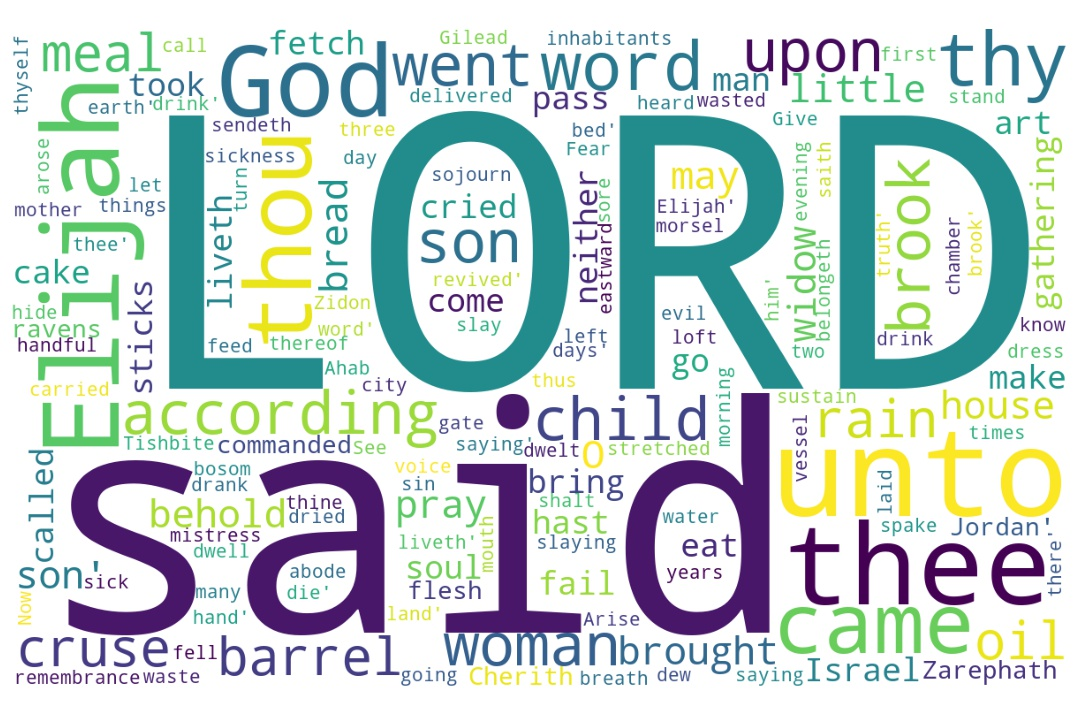
\includegraphics[width=\linewidth]{11OT-1Kings/1Kings17-WordCloud.jpg}
  \caption{1 Kings 17 Word Cloud}
  \label{fig:1 Kings 17 Word Cloud}
\end{figure}

%%%%%%%%%%%%%%%%%%%%%%%%%%%%%%%%%%%%%%%%%
%%%%%%%%%%%%%%%%%%%%%%%%%%%%%%%%%%%%%%%%%

\marginpar{\scriptsize \centering \fcolorbox{bone}{lime}{\textbf{MIRACLES IN ZAREPHATH}}\\ (1 Kings 17) \begin{compactenum}[I.][8]
     \item Elijah's \textbf{Decree} \index[scripture]{1Kings!1Ki 17:01}  (1Ki 17:1) 
    \item Endorsed \textbf{Dwellings} \index[scripture]{1Kings!1Ki 17:03}   \index[scripture]{1Kings!1Ki 17:09} (1Ki 17:3, 9) 
    \item The Extended  \textbf{Drought} \index[scripture]{1Kings!1Ki 17:07}  (1Ki 17:7) 
    \item An Emotional \textbf{Death} \index[scripture]{1Kings!1Ki 17:17}  (1Ki 17:17) 
	\item An Expression of \textbf{Distress} \index[scripture]{1Kings!1Ki 17:18}  (1Ki 17:18) 
   \item An Earnest \textbf{Desire} \index[scripture]{1Kings!1Ki 17:21}  (1Ki 17:21) 
    \item An Exciting \textbf{Deliverance} \index[scripture]{1Kings!1Ki 17:22}  (1Ki 17:22) 
\end{compactenum}}

\footnote{\textcolor[cmyk]{0.99998,1,0,0}{\hyperlink{TOC}{Return to end of Table of Contents.}}}\footnote{\href{https://audiobible.com/bible/1_kings_17.html}{\textcolor[cmyk]{0.99998,1,0,0}{1 Kings 17 Audio}}}\textcolor[cmyk]{0.99998,1,0,0}{And Elijah the Tishbite, \emph{who} \emph{was} \fcolorbox{bone}{bone}{of the} inhabitants of Gilead, said unto Ahab, \emph{As} the LORD God of Israel liveth, before whom \fcolorbox{bone}{bone}{I} stand, there shall not be dew nor rain these years, but according to my word.}
[2] \textcolor[cmyk]{0.99998,1,0,0}{And the word \fcolorbox{bone}{bone}{of the} LORD came unto him, saying,}
[3] \textcolor[cmyk]{0.99998,1,0,0}{Get thee hence, and turn thee eastward, and hide thyself by the brook Cherith, that \emph{is} before Jordan.}
[4] \textcolor[cmyk]{0.99998,1,0,0}{And it shall be, \emph{that} thou shalt drink \fcolorbox{bone}{bone}{of the} brook; and \fcolorbox{bone}{bone}{I} have commanded the ravens to feed thee there.}
[5] \textcolor[cmyk]{0.99998,1,0,0}{So he went and did according unto the word \fcolorbox{bone}{bone}{of the} LORD: for he went and dwelt by the brook Cherith, that \emph{is} before Jordan.}
[6] \textcolor[cmyk]{0.99998,1,0,0}{And the ravens brought him bread and flesh in the morning, and bread and flesh in the evening; and he drank \fcolorbox{bone}{bone}{of the} brook.}
[7] \textcolor[cmyk]{0.99998,1,0,0}{And it came to pass after a while, that the brook dried up, because there had been no rain in the land.}\\
\\
\P  \textcolor[cmyk]{0.99998,1,0,0}{And the word \fcolorbox{bone}{bone}{of the} LORD came unto him, saying,}
[9] \textcolor[cmyk]{0.99998,1,0,0}{Arise, get thee to Zarephath, which \emph{belongeth} to Zidon, and dwell there: behold, \fcolorbox{bone}{bone}{I} have commanded a widow woman there to sustain thee.}
[10] \textcolor[cmyk]{0.99998,1,0,0}{So he arose and went to Zarephath. And when he came to the gate \fcolorbox{bone}{bone}{of the} city, behold, the widow woman \emph{was} there gathering of sticks: and he called to her, and said, Fetch me, \fcolorbox{bone}{bone}{I} pray thee, a little water in a vessel, that \fcolorbox{bone}{bone}{I} may drink.}
[11] \textcolor[cmyk]{0.99998,1,0,0}{And as she was going to fetch \emph{it}, he called to her, and said, Bring me, \fcolorbox{bone}{bone}{I} pray thee, a morsel of bread in thine hand.}
[12] \textcolor[cmyk]{0.99998,1,0,0}{And she said, \emph{As} the LORD thy God liveth, \fcolorbox{bone}{bone}{I} have not a cake, but an handful of meal in a barrel, and a little oil in a cruse: and, behold, \fcolorbox{bone}{bone}{I} \emph{am} gathering two sticks, that \fcolorbox{bone}{bone}{I} may go in and dress it for me and my son, that we may eat it, and die.}
[13] \textcolor[cmyk]{0.99998,1,0,0}{And Elijah said unto her, Fear not; go \emph{and} do as thou hast said: but make me thereof a little cake first, and bring \emph{it} unto me, and after make for thee and for thy son.}
[14] \textcolor[cmyk]{0.99998,1,0,0}{For thus saith the LORD God of Israel, The barrel of meal shall not waste, neither shall the cruse of oil fail, until the day \emph{that} the LORD sendeth rain upon the earth.}
[15] \textcolor[cmyk]{0.99998,1,0,0}{And she went and did according to the saying of Elijah: and she, and he, and her house, did eat \emph{many} days.}
[16] \textcolor[cmyk]{0.99998,1,0,0}{\emph{And} the barrel of meal wasted not, neither did the cruse of oil fail, according to the word \fcolorbox{bone}{bone}{of the} LORD, which he spake by Elijah.}\\
\\
\P  \textcolor[cmyk]{0.99998,1,0,0}{And it came to pass after these things, \emph{that} the son \fcolorbox{bone}{bone}{of the} woman, the mistress \fcolorbox{bone}{bone}{of the} house, fell sick; and his sickness was so sore, that there was no breath left in him.}
[18] \textcolor[cmyk]{0.99998,1,0,0}{And she said unto Elijah, What have \fcolorbox{bone}{bone}{I} to do with thee, O thou man of God? art thou come unto me to call my sin to remembrance, and to slay my son?}
[19] \textcolor[cmyk]{0.99998,1,0,0}{And he said unto her, Give me thy son. And he took him out of her bosom, and carried him up into a loft, where he abode, and laid him upon his own bed.}
[20] \textcolor[cmyk]{0.99998,1,0,0}{And he cried unto the LORD, and said, O LORD my God, hast thou also brought evil upon the widow with whom \fcolorbox{bone}{bone}{I} sojourn, by slaying her son?}
[21] \textcolor[cmyk]{0.99998,1,0,0}{And he stretched himself upon the child three times, and cried unto the LORD, and said, O LORD my God, \fcolorbox{bone}{bone}{I} pray thee, let this child's soul come into him again.}
[22] \textcolor[cmyk]{0.99998,1,0,0}{And the LORD heard the voice of Elijah; and the soul \fcolorbox{bone}{bone}{of the} child came into him again, and he revived.}
[23] \textcolor[cmyk]{0.99998,1,0,0}{And Elijah took the child, and brought him down out \fcolorbox{bone}{bone}{of the} chamber into the house, and delivered him unto his mother: and Elijah said, See, thy son liveth.}\\
\\
\P  \textcolor[cmyk]{0.99998,1,0,0}{And the woman said to Elijah, Now by this \fcolorbox{bone}{bone}{I} know that thou \emph{art} a man of God, \emph{and} that the word \fcolorbox{bone}{bone}{of the} LORD in thy mouth \emph{is} truth.}
\index[NWIV]{39!1Kings!1Ki 17:1}\index[AWIP]{And!1Kings!1Ki 17:1}\index[AWIP]{Elijah!1Kings!1Ki 17:1}\index[AWIP]{the!1Kings!1Ki 17:1}\index[AWIP]{the!1Kings!1Ki 17:1 (2)}\index[AWIP]{the!1Kings!1Ki 17:1 (3)}\index[AWIP]{Tishbite!1Kings!1Ki 17:1}\index[AWIP]{\emph{who}!1Kings!1Ki 17:1}\index[AWIP]{\emph{was}!1Kings!1Ki 17:1}\index[AWIP]{of!1Kings!1Ki 17:1}\index[AWIP]{of!1Kings!1Ki 17:1 (2)}\index[AWIP]{of!1Kings!1Ki 17:1 (3)}\index[AWIP]{inhabitants!1Kings!1Ki 17:1}\index[AWIP]{Gilead!1Kings!1Ki 17:1}\index[AWIP]{said!1Kings!1Ki 17:1}\index[AWIP]{unto!1Kings!1Ki 17:1}\index[AWIP]{Ahab!1Kings!1Ki 17:1}\index[AWIP]{\emph{As}!1Kings!1Ki 17:1}\index[AWIP]{LORD!1Kings!1Ki 17:1}\index[AWIP]{God!1Kings!1Ki 17:1}\index[AWIP]{Israel!1Kings!1Ki 17:1}\index[AWIP]{liveth!1Kings!1Ki 17:1}\index[AWIP]{before!1Kings!1Ki 17:1}\index[AWIP]{whom!1Kings!1Ki 17:1}\index[AWIP]{I!1Kings!1Ki 17:1}\index[AWIP]{stand!1Kings!1Ki 17:1}\index[AWIP]{there!1Kings!1Ki 17:1}\index[AWIP]{shall!1Kings!1Ki 17:1}\index[AWIP]{not!1Kings!1Ki 17:1}\index[AWIP]{be!1Kings!1Ki 17:1}\index[AWIP]{dew!1Kings!1Ki 17:1}\index[AWIP]{nor!1Kings!1Ki 17:1}\index[AWIP]{rain!1Kings!1Ki 17:1}\index[AWIP]{these!1Kings!1Ki 17:1}\index[AWIP]{years!1Kings!1Ki 17:1}\index[AWIP]{but!1Kings!1Ki 17:1}\index[AWIP]{according!1Kings!1Ki 17:1}\index[AWIP]{to!1Kings!1Ki 17:1}\index[AWIP]{my!1Kings!1Ki 17:1}\index[AWIP]{word!1Kings!1Ki 17:1}\index[AWIP]{\emph{who}!1Kings!1Ki 17:1}\index[AWIP]{\emph{was}!1Kings!1Ki 17:1}\index[AWIP]{\emph{As}!1Kings!1Ki 17:1}

\index[NWIV]{10!1Kings!1Ki 17:2}\index[AWIP]{And!1Kings!1Ki 17:2}\index[AWIP]{the!1Kings!1Ki 17:2}\index[AWIP]{the!1Kings!1Ki 17:2 (2)}\index[AWIP]{word!1Kings!1Ki 17:2}\index[AWIP]{of!1Kings!1Ki 17:2}\index[AWIP]{LORD!1Kings!1Ki 17:2}\index[AWIP]{came!1Kings!1Ki 17:2}\index[AWIP]{unto!1Kings!1Ki 17:2}\index[AWIP]{him!1Kings!1Ki 17:2}\index[AWIP]{saying!1Kings!1Ki 17:2}

\index[NWIV]{18!1Kings!1Ki 17:3}\index[AWIP]{Get!1Kings!1Ki 17:3}\index[AWIP]{thee!1Kings!1Ki 17:3}\index[AWIP]{thee!1Kings!1Ki 17:3 (2)}\index[AWIP]{hence!1Kings!1Ki 17:3}\index[AWIP]{and!1Kings!1Ki 17:3}\index[AWIP]{and!1Kings!1Ki 17:3 (2)}\index[AWIP]{turn!1Kings!1Ki 17:3}\index[AWIP]{eastward!1Kings!1Ki 17:3}\index[AWIP]{hide!1Kings!1Ki 17:3}\index[AWIP]{thyself!1Kings!1Ki 17:3}\index[AWIP]{by!1Kings!1Ki 17:3}\index[AWIP]{the!1Kings!1Ki 17:3}\index[AWIP]{brook!1Kings!1Ki 17:3}\index[AWIP]{Cherith!1Kings!1Ki 17:3}\index[AWIP]{that!1Kings!1Ki 17:3}\index[AWIP]{\emph{is}!1Kings!1Ki 17:3}\index[AWIP]{before!1Kings!1Ki 17:3}\index[AWIP]{Jordan!1Kings!1Ki 17:3}\index[AWIP]{\emph{is}!1Kings!1Ki 17:3}

\index[NWIV]{21!1Kings!1Ki 17:4}\index[AWIP]{And!1Kings!1Ki 17:4}\index[AWIP]{it!1Kings!1Ki 17:4}\index[AWIP]{shall!1Kings!1Ki 17:4}\index[AWIP]{be!1Kings!1Ki 17:4}\index[AWIP]{\emph{that}!1Kings!1Ki 17:4}\index[AWIP]{thou!1Kings!1Ki 17:4}\index[AWIP]{shalt!1Kings!1Ki 17:4}\index[AWIP]{drink!1Kings!1Ki 17:4}\index[AWIP]{of!1Kings!1Ki 17:4}\index[AWIP]{the!1Kings!1Ki 17:4}\index[AWIP]{the!1Kings!1Ki 17:4 (2)}\index[AWIP]{brook!1Kings!1Ki 17:4}\index[AWIP]{and!1Kings!1Ki 17:4}\index[AWIP]{I!1Kings!1Ki 17:4}\index[AWIP]{have!1Kings!1Ki 17:4}\index[AWIP]{commanded!1Kings!1Ki 17:4}\index[AWIP]{ravens!1Kings!1Ki 17:4}\index[AWIP]{to!1Kings!1Ki 17:4}\index[AWIP]{feed!1Kings!1Ki 17:4}\index[AWIP]{thee!1Kings!1Ki 17:4}\index[AWIP]{there!1Kings!1Ki 17:4}\index[AWIP]{\emph{that}!1Kings!1Ki 17:4}

\index[NWIV]{25!1Kings!1Ki 17:5}\index[AWIP]{So!1Kings!1Ki 17:5}\index[AWIP]{he!1Kings!1Ki 17:5}\index[AWIP]{he!1Kings!1Ki 17:5 (2)}\index[AWIP]{went!1Kings!1Ki 17:5}\index[AWIP]{went!1Kings!1Ki 17:5 (2)}\index[AWIP]{and!1Kings!1Ki 17:5}\index[AWIP]{and!1Kings!1Ki 17:5 (2)}\index[AWIP]{did!1Kings!1Ki 17:5}\index[AWIP]{according!1Kings!1Ki 17:5}\index[AWIP]{unto!1Kings!1Ki 17:5}\index[AWIP]{the!1Kings!1Ki 17:5}\index[AWIP]{the!1Kings!1Ki 17:5 (2)}\index[AWIP]{the!1Kings!1Ki 17:5 (3)}\index[AWIP]{word!1Kings!1Ki 17:5}\index[AWIP]{of!1Kings!1Ki 17:5}\index[AWIP]{LORD!1Kings!1Ki 17:5}\index[AWIP]{for!1Kings!1Ki 17:5}\index[AWIP]{dwelt!1Kings!1Ki 17:5}\index[AWIP]{by!1Kings!1Ki 17:5}\index[AWIP]{brook!1Kings!1Ki 17:5}\index[AWIP]{Cherith!1Kings!1Ki 17:5}\index[AWIP]{that!1Kings!1Ki 17:5}\index[AWIP]{\emph{is}!1Kings!1Ki 17:5}\index[AWIP]{before!1Kings!1Ki 17:5}\index[AWIP]{Jordan!1Kings!1Ki 17:5}\index[AWIP]{\emph{is}!1Kings!1Ki 17:5}

\index[NWIV]{24!1Kings!1Ki 17:6}\index[AWIP]{And!1Kings!1Ki 17:6}\index[AWIP]{the!1Kings!1Ki 17:6}\index[AWIP]{the!1Kings!1Ki 17:6 (2)}\index[AWIP]{the!1Kings!1Ki 17:6 (3)}\index[AWIP]{the!1Kings!1Ki 17:6 (4)}\index[AWIP]{ravens!1Kings!1Ki 17:6}\index[AWIP]{brought!1Kings!1Ki 17:6}\index[AWIP]{him!1Kings!1Ki 17:6}\index[AWIP]{bread!1Kings!1Ki 17:6}\index[AWIP]{bread!1Kings!1Ki 17:6 (2)}\index[AWIP]{and!1Kings!1Ki 17:6}\index[AWIP]{and!1Kings!1Ki 17:6 (2)}\index[AWIP]{and!1Kings!1Ki 17:6 (3)}\index[AWIP]{and!1Kings!1Ki 17:6 (4)}\index[AWIP]{flesh!1Kings!1Ki 17:6}\index[AWIP]{flesh!1Kings!1Ki 17:6 (2)}\index[AWIP]{in!1Kings!1Ki 17:6}\index[AWIP]{in!1Kings!1Ki 17:6 (2)}\index[AWIP]{morning!1Kings!1Ki 17:6}\index[AWIP]{evening!1Kings!1Ki 17:6}\index[AWIP]{he!1Kings!1Ki 17:6}\index[AWIP]{drank!1Kings!1Ki 17:6}\index[AWIP]{of!1Kings!1Ki 17:6}\index[AWIP]{brook!1Kings!1Ki 17:6}

\index[NWIV]{22!1Kings!1Ki 17:7}\index[AWIP]{And!1Kings!1Ki 17:7}\index[AWIP]{it!1Kings!1Ki 17:7}\index[AWIP]{came!1Kings!1Ki 17:7}\index[AWIP]{to!1Kings!1Ki 17:7}\index[AWIP]{pass!1Kings!1Ki 17:7}\index[AWIP]{after!1Kings!1Ki 17:7}\index[AWIP]{a!1Kings!1Ki 17:7}\index[AWIP]{while!1Kings!1Ki 17:7}\index[AWIP]{that!1Kings!1Ki 17:7}\index[AWIP]{the!1Kings!1Ki 17:7}\index[AWIP]{the!1Kings!1Ki 17:7 (2)}\index[AWIP]{brook!1Kings!1Ki 17:7}\index[AWIP]{dried!1Kings!1Ki 17:7}\index[AWIP]{up!1Kings!1Ki 17:7}\index[AWIP]{because!1Kings!1Ki 17:7}\index[AWIP]{there!1Kings!1Ki 17:7}\index[AWIP]{had!1Kings!1Ki 17:7}\index[AWIP]{been!1Kings!1Ki 17:7}\index[AWIP]{no!1Kings!1Ki 17:7}\index[AWIP]{rain!1Kings!1Ki 17:7}\index[AWIP]{in!1Kings!1Ki 17:7}\index[AWIP]{land!1Kings!1Ki 17:7}

\index[NWIV]{10!1Kings!1Ki 17:8}\index[AWIP]{And!1Kings!1Ki 17:8}\index[AWIP]{the!1Kings!1Ki 17:8}\index[AWIP]{the!1Kings!1Ki 17:8 (2)}\index[AWIP]{word!1Kings!1Ki 17:8}\index[AWIP]{of!1Kings!1Ki 17:8}\index[AWIP]{LORD!1Kings!1Ki 17:8}\index[AWIP]{came!1Kings!1Ki 17:8}\index[AWIP]{unto!1Kings!1Ki 17:8}\index[AWIP]{him!1Kings!1Ki 17:8}\index[AWIP]{saying!1Kings!1Ki 17:8}

\index[NWIV]{23!1Kings!1Ki 17:9}\index[AWIP]{Arise!1Kings!1Ki 17:9}\index[AWIP]{get!1Kings!1Ki 17:9}\index[AWIP]{thee!1Kings!1Ki 17:9}\index[AWIP]{thee!1Kings!1Ki 17:9 (2)}\index[AWIP]{to!1Kings!1Ki 17:9}\index[AWIP]{to!1Kings!1Ki 17:9 (2)}\index[AWIP]{to!1Kings!1Ki 17:9 (3)}\index[AWIP]{Zarephath!1Kings!1Ki 17:9}\index[AWIP]{which!1Kings!1Ki 17:9}\index[AWIP]{\emph{belongeth}!1Kings!1Ki 17:9}\index[AWIP]{Zidon!1Kings!1Ki 17:9}\index[AWIP]{and!1Kings!1Ki 17:9}\index[AWIP]{dwell!1Kings!1Ki 17:9}\index[AWIP]{there!1Kings!1Ki 17:9}\index[AWIP]{there!1Kings!1Ki 17:9 (2)}\index[AWIP]{behold!1Kings!1Ki 17:9}\index[AWIP]{I!1Kings!1Ki 17:9}\index[AWIP]{have!1Kings!1Ki 17:9}\index[AWIP]{commanded!1Kings!1Ki 17:9}\index[AWIP]{a!1Kings!1Ki 17:9}\index[AWIP]{widow!1Kings!1Ki 17:9}\index[AWIP]{woman!1Kings!1Ki 17:9}\index[AWIP]{sustain!1Kings!1Ki 17:9}\index[AWIP]{\emph{belongeth}!1Kings!1Ki 17:9}

\index[NWIV]{48!1Kings!1Ki 17:10}\index[AWIP]{So!1Kings!1Ki 17:10}\index[AWIP]{he!1Kings!1Ki 17:10}\index[AWIP]{he!1Kings!1Ki 17:10 (2)}\index[AWIP]{he!1Kings!1Ki 17:10 (3)}\index[AWIP]{arose!1Kings!1Ki 17:10}\index[AWIP]{and!1Kings!1Ki 17:10}\index[AWIP]{and!1Kings!1Ki 17:10 (2)}\index[AWIP]{and!1Kings!1Ki 17:10 (3)}\index[AWIP]{went!1Kings!1Ki 17:10}\index[AWIP]{to!1Kings!1Ki 17:10}\index[AWIP]{to!1Kings!1Ki 17:10 (2)}\index[AWIP]{to!1Kings!1Ki 17:10 (3)}\index[AWIP]{Zarephath!1Kings!1Ki 17:10}\index[AWIP]{And!1Kings!1Ki 17:10}\index[AWIP]{when!1Kings!1Ki 17:10}\index[AWIP]{came!1Kings!1Ki 17:10}\index[AWIP]{the!1Kings!1Ki 17:10}\index[AWIP]{the!1Kings!1Ki 17:10 (2)}\index[AWIP]{the!1Kings!1Ki 17:10 (3)}\index[AWIP]{gate!1Kings!1Ki 17:10}\index[AWIP]{of!1Kings!1Ki 17:10}\index[AWIP]{of!1Kings!1Ki 17:10 (2)}\index[AWIP]{city!1Kings!1Ki 17:10}\index[AWIP]{behold!1Kings!1Ki 17:10}\index[AWIP]{widow!1Kings!1Ki 17:10}\index[AWIP]{woman!1Kings!1Ki 17:10}\index[AWIP]{\emph{was}!1Kings!1Ki 17:10}\index[AWIP]{there!1Kings!1Ki 17:10}\index[AWIP]{gathering!1Kings!1Ki 17:10}\index[AWIP]{sticks!1Kings!1Ki 17:10}\index[AWIP]{called!1Kings!1Ki 17:10}\index[AWIP]{her!1Kings!1Ki 17:10}\index[AWIP]{said!1Kings!1Ki 17:10}\index[AWIP]{Fetch!1Kings!1Ki 17:10}\index[AWIP]{me!1Kings!1Ki 17:10}\index[AWIP]{I!1Kings!1Ki 17:10}\index[AWIP]{I!1Kings!1Ki 17:10 (2)}\index[AWIP]{pray!1Kings!1Ki 17:10}\index[AWIP]{thee!1Kings!1Ki 17:10}\index[AWIP]{a!1Kings!1Ki 17:10}\index[AWIP]{a!1Kings!1Ki 17:10 (2)}\index[AWIP]{little!1Kings!1Ki 17:10}\index[AWIP]{water!1Kings!1Ki 17:10}\index[AWIP]{in!1Kings!1Ki 17:10}\index[AWIP]{vessel!1Kings!1Ki 17:10}\index[AWIP]{that!1Kings!1Ki 17:10}\index[AWIP]{may!1Kings!1Ki 17:10}\index[AWIP]{drink!1Kings!1Ki 17:10}\index[AWIP]{\emph{was}!1Kings!1Ki 17:10}

\index[NWIV]{26!1Kings!1Ki 17:11}\index[AWIP]{And!1Kings!1Ki 17:11}\index[AWIP]{as!1Kings!1Ki 17:11}\index[AWIP]{she!1Kings!1Ki 17:11}\index[AWIP]{was!1Kings!1Ki 17:11}\index[AWIP]{going!1Kings!1Ki 17:11}\index[AWIP]{to!1Kings!1Ki 17:11}\index[AWIP]{to!1Kings!1Ki 17:11 (2)}\index[AWIP]{fetch!1Kings!1Ki 17:11}\index[AWIP]{\emph{it}!1Kings!1Ki 17:11}\index[AWIP]{he!1Kings!1Ki 17:11}\index[AWIP]{called!1Kings!1Ki 17:11}\index[AWIP]{her!1Kings!1Ki 17:11}\index[AWIP]{and!1Kings!1Ki 17:11}\index[AWIP]{said!1Kings!1Ki 17:11}\index[AWIP]{Bring!1Kings!1Ki 17:11}\index[AWIP]{me!1Kings!1Ki 17:11}\index[AWIP]{I!1Kings!1Ki 17:11}\index[AWIP]{pray!1Kings!1Ki 17:11}\index[AWIP]{thee!1Kings!1Ki 17:11}\index[AWIP]{a!1Kings!1Ki 17:11}\index[AWIP]{morsel!1Kings!1Ki 17:11}\index[AWIP]{of!1Kings!1Ki 17:11}\index[AWIP]{bread!1Kings!1Ki 17:11}\index[AWIP]{in!1Kings!1Ki 17:11}\index[AWIP]{thine!1Kings!1Ki 17:11}\index[AWIP]{hand!1Kings!1Ki 17:11}\index[AWIP]{\emph{it}!1Kings!1Ki 17:11}

\index[NWIV]{56!1Kings!1Ki 17:12}\index[AWIP]{And!1Kings!1Ki 17:12}\index[AWIP]{she!1Kings!1Ki 17:12}\index[AWIP]{said!1Kings!1Ki 17:12}\index[AWIP]{\emph{As}!1Kings!1Ki 17:12}\index[AWIP]{the!1Kings!1Ki 17:12}\index[AWIP]{LORD!1Kings!1Ki 17:12}\index[AWIP]{thy!1Kings!1Ki 17:12}\index[AWIP]{God!1Kings!1Ki 17:12}\index[AWIP]{liveth!1Kings!1Ki 17:12}\index[AWIP]{I!1Kings!1Ki 17:12}\index[AWIP]{I!1Kings!1Ki 17:12 (2)}\index[AWIP]{I!1Kings!1Ki 17:12 (3)}\index[AWIP]{have!1Kings!1Ki 17:12}\index[AWIP]{not!1Kings!1Ki 17:12}\index[AWIP]{a!1Kings!1Ki 17:12}\index[AWIP]{a!1Kings!1Ki 17:12 (2)}\index[AWIP]{a!1Kings!1Ki 17:12 (3)}\index[AWIP]{a!1Kings!1Ki 17:12 (4)}\index[AWIP]{cake!1Kings!1Ki 17:12}\index[AWIP]{but!1Kings!1Ki 17:12}\index[AWIP]{an!1Kings!1Ki 17:12}\index[AWIP]{handful!1Kings!1Ki 17:12}\index[AWIP]{of!1Kings!1Ki 17:12}\index[AWIP]{meal!1Kings!1Ki 17:12}\index[AWIP]{in!1Kings!1Ki 17:12}\index[AWIP]{in!1Kings!1Ki 17:12 (2)}\index[AWIP]{in!1Kings!1Ki 17:12 (3)}\index[AWIP]{barrel!1Kings!1Ki 17:12}\index[AWIP]{and!1Kings!1Ki 17:12}\index[AWIP]{and!1Kings!1Ki 17:12 (2)}\index[AWIP]{and!1Kings!1Ki 17:12 (3)}\index[AWIP]{and!1Kings!1Ki 17:12 (4)}\index[AWIP]{and!1Kings!1Ki 17:12 (5)}\index[AWIP]{little!1Kings!1Ki 17:12}\index[AWIP]{oil!1Kings!1Ki 17:12}\index[AWIP]{cruse!1Kings!1Ki 17:12}\index[AWIP]{behold!1Kings!1Ki 17:12}\index[AWIP]{\emph{am}!1Kings!1Ki 17:12}\index[AWIP]{gathering!1Kings!1Ki 17:12}\index[AWIP]{two!1Kings!1Ki 17:12}\index[AWIP]{sticks!1Kings!1Ki 17:12}\index[AWIP]{that!1Kings!1Ki 17:12}\index[AWIP]{that!1Kings!1Ki 17:12 (2)}\index[AWIP]{may!1Kings!1Ki 17:12}\index[AWIP]{may!1Kings!1Ki 17:12 (2)}\index[AWIP]{go!1Kings!1Ki 17:12}\index[AWIP]{dress!1Kings!1Ki 17:12}\index[AWIP]{it!1Kings!1Ki 17:12}\index[AWIP]{it!1Kings!1Ki 17:12 (2)}\index[AWIP]{for!1Kings!1Ki 17:12}\index[AWIP]{me!1Kings!1Ki 17:12}\index[AWIP]{my!1Kings!1Ki 17:12}\index[AWIP]{son!1Kings!1Ki 17:12}\index[AWIP]{we!1Kings!1Ki 17:12}\index[AWIP]{eat!1Kings!1Ki 17:12}\index[AWIP]{die!1Kings!1Ki 17:12}\index[AWIP]{\emph{As}!1Kings!1Ki 17:12}\index[AWIP]{\emph{am}!1Kings!1Ki 17:12}

\index[NWIV]{36!1Kings!1Ki 17:13}\index[AWIP]{And!1Kings!1Ki 17:13}\index[AWIP]{Elijah!1Kings!1Ki 17:13}\index[AWIP]{said!1Kings!1Ki 17:13}\index[AWIP]{said!1Kings!1Ki 17:13 (2)}\index[AWIP]{unto!1Kings!1Ki 17:13}\index[AWIP]{unto!1Kings!1Ki 17:13 (2)}\index[AWIP]{her!1Kings!1Ki 17:13}\index[AWIP]{Fear!1Kings!1Ki 17:13}\index[AWIP]{not!1Kings!1Ki 17:13}\index[AWIP]{go!1Kings!1Ki 17:13}\index[AWIP]{\emph{and}!1Kings!1Ki 17:13}\index[AWIP]{do!1Kings!1Ki 17:13}\index[AWIP]{as!1Kings!1Ki 17:13}\index[AWIP]{thou!1Kings!1Ki 17:13}\index[AWIP]{hast!1Kings!1Ki 17:13}\index[AWIP]{but!1Kings!1Ki 17:13}\index[AWIP]{make!1Kings!1Ki 17:13}\index[AWIP]{make!1Kings!1Ki 17:13 (2)}\index[AWIP]{me!1Kings!1Ki 17:13}\index[AWIP]{me!1Kings!1Ki 17:13 (2)}\index[AWIP]{thereof!1Kings!1Ki 17:13}\index[AWIP]{a!1Kings!1Ki 17:13}\index[AWIP]{little!1Kings!1Ki 17:13}\index[AWIP]{cake!1Kings!1Ki 17:13}\index[AWIP]{first!1Kings!1Ki 17:13}\index[AWIP]{and!1Kings!1Ki 17:13}\index[AWIP]{and!1Kings!1Ki 17:13 (2)}\index[AWIP]{and!1Kings!1Ki 17:13 (3)}\index[AWIP]{bring!1Kings!1Ki 17:13}\index[AWIP]{\emph{it}!1Kings!1Ki 17:13}\index[AWIP]{after!1Kings!1Ki 17:13}\index[AWIP]{for!1Kings!1Ki 17:13}\index[AWIP]{for!1Kings!1Ki 17:13 (2)}\index[AWIP]{thee!1Kings!1Ki 17:13}\index[AWIP]{thy!1Kings!1Ki 17:13}\index[AWIP]{son!1Kings!1Ki 17:13}\index[AWIP]{\emph{and}!1Kings!1Ki 17:13}\index[AWIP]{\emph{it}!1Kings!1Ki 17:13}

\index[NWIV]{33!1Kings!1Ki 17:14}\index[AWIP]{For!1Kings!1Ki 17:14}\index[AWIP]{thus!1Kings!1Ki 17:14}\index[AWIP]{saith!1Kings!1Ki 17:14}\index[AWIP]{the!1Kings!1Ki 17:14}\index[AWIP]{the!1Kings!1Ki 17:14 (2)}\index[AWIP]{the!1Kings!1Ki 17:14 (3)}\index[AWIP]{the!1Kings!1Ki 17:14 (4)}\index[AWIP]{the!1Kings!1Ki 17:14 (5)}\index[AWIP]{LORD!1Kings!1Ki 17:14}\index[AWIP]{LORD!1Kings!1Ki 17:14 (2)}\index[AWIP]{God!1Kings!1Ki 17:14}\index[AWIP]{of!1Kings!1Ki 17:14}\index[AWIP]{of!1Kings!1Ki 17:14 (2)}\index[AWIP]{of!1Kings!1Ki 17:14 (3)}\index[AWIP]{Israel!1Kings!1Ki 17:14}\index[AWIP]{The!1Kings!1Ki 17:14}\index[AWIP]{barrel!1Kings!1Ki 17:14}\index[AWIP]{meal!1Kings!1Ki 17:14}\index[AWIP]{shall!1Kings!1Ki 17:14}\index[AWIP]{shall!1Kings!1Ki 17:14 (2)}\index[AWIP]{not!1Kings!1Ki 17:14}\index[AWIP]{waste!1Kings!1Ki 17:14}\index[AWIP]{neither!1Kings!1Ki 17:14}\index[AWIP]{cruse!1Kings!1Ki 17:14}\index[AWIP]{oil!1Kings!1Ki 17:14}\index[AWIP]{fail!1Kings!1Ki 17:14}\index[AWIP]{until!1Kings!1Ki 17:14}\index[AWIP]{day!1Kings!1Ki 17:14}\index[AWIP]{\emph{that}!1Kings!1Ki 17:14}\index[AWIP]{sendeth!1Kings!1Ki 17:14}\index[AWIP]{rain!1Kings!1Ki 17:14}\index[AWIP]{upon!1Kings!1Ki 17:14}\index[AWIP]{earth!1Kings!1Ki 17:14}\index[AWIP]{\emph{that}!1Kings!1Ki 17:14}

\index[NWIV]{22!1Kings!1Ki 17:15}\index[AWIP]{And!1Kings!1Ki 17:15}\index[AWIP]{she!1Kings!1Ki 17:15}\index[AWIP]{she!1Kings!1Ki 17:15 (2)}\index[AWIP]{went!1Kings!1Ki 17:15}\index[AWIP]{and!1Kings!1Ki 17:15}\index[AWIP]{and!1Kings!1Ki 17:15 (2)}\index[AWIP]{and!1Kings!1Ki 17:15 (3)}\index[AWIP]{and!1Kings!1Ki 17:15 (4)}\index[AWIP]{did!1Kings!1Ki 17:15}\index[AWIP]{did!1Kings!1Ki 17:15 (2)}\index[AWIP]{according!1Kings!1Ki 17:15}\index[AWIP]{to!1Kings!1Ki 17:15}\index[AWIP]{the!1Kings!1Ki 17:15}\index[AWIP]{saying!1Kings!1Ki 17:15}\index[AWIP]{of!1Kings!1Ki 17:15}\index[AWIP]{Elijah!1Kings!1Ki 17:15}\index[AWIP]{he!1Kings!1Ki 17:15}\index[AWIP]{her!1Kings!1Ki 17:15}\index[AWIP]{house!1Kings!1Ki 17:15}\index[AWIP]{eat!1Kings!1Ki 17:15}\index[AWIP]{\emph{many}!1Kings!1Ki 17:15}\index[AWIP]{days!1Kings!1Ki 17:15}\index[AWIP]{\emph{many}!1Kings!1Ki 17:15}

\index[NWIV]{26!1Kings!1Ki 17:16}\index[AWIP]{\emph{And}!1Kings!1Ki 17:16}\index[AWIP]{the!1Kings!1Ki 17:16}\index[AWIP]{the!1Kings!1Ki 17:16 (2)}\index[AWIP]{the!1Kings!1Ki 17:16 (3)}\index[AWIP]{the!1Kings!1Ki 17:16 (4)}\index[AWIP]{barrel!1Kings!1Ki 17:16}\index[AWIP]{of!1Kings!1Ki 17:16}\index[AWIP]{of!1Kings!1Ki 17:16 (2)}\index[AWIP]{of!1Kings!1Ki 17:16 (3)}\index[AWIP]{meal!1Kings!1Ki 17:16}\index[AWIP]{wasted!1Kings!1Ki 17:16}\index[AWIP]{not!1Kings!1Ki 17:16}\index[AWIP]{neither!1Kings!1Ki 17:16}\index[AWIP]{did!1Kings!1Ki 17:16}\index[AWIP]{cruse!1Kings!1Ki 17:16}\index[AWIP]{oil!1Kings!1Ki 17:16}\index[AWIP]{fail!1Kings!1Ki 17:16}\index[AWIP]{according!1Kings!1Ki 17:16}\index[AWIP]{to!1Kings!1Ki 17:16}\index[AWIP]{word!1Kings!1Ki 17:16}\index[AWIP]{LORD!1Kings!1Ki 17:16}\index[AWIP]{which!1Kings!1Ki 17:16}\index[AWIP]{he!1Kings!1Ki 17:16}\index[AWIP]{spake!1Kings!1Ki 17:16}\index[AWIP]{by!1Kings!1Ki 17:16}\index[AWIP]{Elijah!1Kings!1Ki 17:16}\index[AWIP]{\emph{And}!1Kings!1Ki 17:16}

\index[NWIV]{35!1Kings!1Ki 17:17}\index[AWIP]{And!1Kings!1Ki 17:17}\index[AWIP]{it!1Kings!1Ki 17:17}\index[AWIP]{came!1Kings!1Ki 17:17}\index[AWIP]{to!1Kings!1Ki 17:17}\index[AWIP]{pass!1Kings!1Ki 17:17}\index[AWIP]{after!1Kings!1Ki 17:17}\index[AWIP]{these!1Kings!1Ki 17:17}\index[AWIP]{things!1Kings!1Ki 17:17}\index[AWIP]{\emph{that}!1Kings!1Ki 17:17}\index[AWIP]{the!1Kings!1Ki 17:17}\index[AWIP]{the!1Kings!1Ki 17:17 (2)}\index[AWIP]{the!1Kings!1Ki 17:17 (3)}\index[AWIP]{the!1Kings!1Ki 17:17 (4)}\index[AWIP]{son!1Kings!1Ki 17:17}\index[AWIP]{of!1Kings!1Ki 17:17}\index[AWIP]{of!1Kings!1Ki 17:17 (2)}\index[AWIP]{woman!1Kings!1Ki 17:17}\index[AWIP]{mistress!1Kings!1Ki 17:17}\index[AWIP]{house!1Kings!1Ki 17:17}\index[AWIP]{fell!1Kings!1Ki 17:17}\index[AWIP]{sick!1Kings!1Ki 17:17}\index[AWIP]{and!1Kings!1Ki 17:17}\index[AWIP]{his!1Kings!1Ki 17:17}\index[AWIP]{sickness!1Kings!1Ki 17:17}\index[AWIP]{was!1Kings!1Ki 17:17}\index[AWIP]{was!1Kings!1Ki 17:17 (2)}\index[AWIP]{so!1Kings!1Ki 17:17}\index[AWIP]{sore!1Kings!1Ki 17:17}\index[AWIP]{that!1Kings!1Ki 17:17}\index[AWIP]{there!1Kings!1Ki 17:17}\index[AWIP]{no!1Kings!1Ki 17:17}\index[AWIP]{breath!1Kings!1Ki 17:17}\index[AWIP]{left!1Kings!1Ki 17:17}\index[AWIP]{in!1Kings!1Ki 17:17}\index[AWIP]{him!1Kings!1Ki 17:17}\index[AWIP]{\emph{that}!1Kings!1Ki 17:17}

\index[NWIV]{33!1Kings!1Ki 17:18}\index[AWIP]{And!1Kings!1Ki 17:18}\index[AWIP]{she!1Kings!1Ki 17:18}\index[AWIP]{said!1Kings!1Ki 17:18}\index[AWIP]{unto!1Kings!1Ki 17:18}\index[AWIP]{unto!1Kings!1Ki 17:18 (2)}\index[AWIP]{Elijah!1Kings!1Ki 17:18}\index[AWIP]{What!1Kings!1Ki 17:18}\index[AWIP]{have!1Kings!1Ki 17:18}\index[AWIP]{I!1Kings!1Ki 17:18}\index[AWIP]{to!1Kings!1Ki 17:18}\index[AWIP]{to!1Kings!1Ki 17:18 (2)}\index[AWIP]{to!1Kings!1Ki 17:18 (3)}\index[AWIP]{to!1Kings!1Ki 17:18 (4)}\index[AWIP]{do!1Kings!1Ki 17:18}\index[AWIP]{with!1Kings!1Ki 17:18}\index[AWIP]{thee!1Kings!1Ki 17:18}\index[AWIP]{O!1Kings!1Ki 17:18}\index[AWIP]{thou!1Kings!1Ki 17:18}\index[AWIP]{thou!1Kings!1Ki 17:18 (2)}\index[AWIP]{man!1Kings!1Ki 17:18}\index[AWIP]{of!1Kings!1Ki 17:18}\index[AWIP]{God?!1Kings!1Ki 17:18}\index[AWIP]{art!1Kings!1Ki 17:18}\index[AWIP]{come!1Kings!1Ki 17:18}\index[AWIP]{me!1Kings!1Ki 17:18}\index[AWIP]{call!1Kings!1Ki 17:18}\index[AWIP]{my!1Kings!1Ki 17:18}\index[AWIP]{my!1Kings!1Ki 17:18 (2)}\index[AWIP]{sin!1Kings!1Ki 17:18}\index[AWIP]{remembrance!1Kings!1Ki 17:18}\index[AWIP]{and!1Kings!1Ki 17:18}\index[AWIP]{slay!1Kings!1Ki 17:18}\index[AWIP]{son?!1Kings!1Ki 17:18}

\index[NWIV]{34!1Kings!1Ki 17:19}\index[AWIP]{And!1Kings!1Ki 17:19}\index[AWIP]{And!1Kings!1Ki 17:19 (2)}\index[AWIP]{he!1Kings!1Ki 17:19}\index[AWIP]{he!1Kings!1Ki 17:19 (2)}\index[AWIP]{he!1Kings!1Ki 17:19 (3)}\index[AWIP]{said!1Kings!1Ki 17:19}\index[AWIP]{unto!1Kings!1Ki 17:19}\index[AWIP]{her!1Kings!1Ki 17:19}\index[AWIP]{her!1Kings!1Ki 17:19 (2)}\index[AWIP]{Give!1Kings!1Ki 17:19}\index[AWIP]{me!1Kings!1Ki 17:19}\index[AWIP]{thy!1Kings!1Ki 17:19}\index[AWIP]{son!1Kings!1Ki 17:19}\index[AWIP]{took!1Kings!1Ki 17:19}\index[AWIP]{him!1Kings!1Ki 17:19}\index[AWIP]{him!1Kings!1Ki 17:19 (2)}\index[AWIP]{him!1Kings!1Ki 17:19 (3)}\index[AWIP]{out!1Kings!1Ki 17:19}\index[AWIP]{of!1Kings!1Ki 17:19}\index[AWIP]{bosom!1Kings!1Ki 17:19}\index[AWIP]{and!1Kings!1Ki 17:19}\index[AWIP]{and!1Kings!1Ki 17:19 (2)}\index[AWIP]{carried!1Kings!1Ki 17:19}\index[AWIP]{up!1Kings!1Ki 17:19}\index[AWIP]{into!1Kings!1Ki 17:19}\index[AWIP]{a!1Kings!1Ki 17:19}\index[AWIP]{loft!1Kings!1Ki 17:19}\index[AWIP]{where!1Kings!1Ki 17:19}\index[AWIP]{abode!1Kings!1Ki 17:19}\index[AWIP]{laid!1Kings!1Ki 17:19}\index[AWIP]{upon!1Kings!1Ki 17:19}\index[AWIP]{his!1Kings!1Ki 17:19}\index[AWIP]{own!1Kings!1Ki 17:19}\index[AWIP]{bed!1Kings!1Ki 17:19}

\index[NWIV]{28!1Kings!1Ki 17:20}\index[AWIP]{And!1Kings!1Ki 17:20}\index[AWIP]{he!1Kings!1Ki 17:20}\index[AWIP]{cried!1Kings!1Ki 17:20}\index[AWIP]{unto!1Kings!1Ki 17:20}\index[AWIP]{the!1Kings!1Ki 17:20}\index[AWIP]{the!1Kings!1Ki 17:20 (2)}\index[AWIP]{LORD!1Kings!1Ki 17:20}\index[AWIP]{LORD!1Kings!1Ki 17:20 (2)}\index[AWIP]{and!1Kings!1Ki 17:20}\index[AWIP]{said!1Kings!1Ki 17:20}\index[AWIP]{O!1Kings!1Ki 17:20}\index[AWIP]{my!1Kings!1Ki 17:20}\index[AWIP]{God!1Kings!1Ki 17:20}\index[AWIP]{hast!1Kings!1Ki 17:20}\index[AWIP]{thou!1Kings!1Ki 17:20}\index[AWIP]{also!1Kings!1Ki 17:20}\index[AWIP]{brought!1Kings!1Ki 17:20}\index[AWIP]{evil!1Kings!1Ki 17:20}\index[AWIP]{upon!1Kings!1Ki 17:20}\index[AWIP]{widow!1Kings!1Ki 17:20}\index[AWIP]{with!1Kings!1Ki 17:20}\index[AWIP]{whom!1Kings!1Ki 17:20}\index[AWIP]{I!1Kings!1Ki 17:20}\index[AWIP]{sojourn!1Kings!1Ki 17:20}\index[AWIP]{by!1Kings!1Ki 17:20}\index[AWIP]{slaying!1Kings!1Ki 17:20}\index[AWIP]{her!1Kings!1Ki 17:20}\index[AWIP]{son?!1Kings!1Ki 17:20}

\index[NWIV]{31!1Kings!1Ki 17:21}\index[AWIP]{And!1Kings!1Ki 17:21}\index[AWIP]{he!1Kings!1Ki 17:21}\index[AWIP]{stretched!1Kings!1Ki 17:21}\index[AWIP]{himself!1Kings!1Ki 17:21}\index[AWIP]{upon!1Kings!1Ki 17:21}\index[AWIP]{the!1Kings!1Ki 17:21}\index[AWIP]{the!1Kings!1Ki 17:21 (2)}\index[AWIP]{child!1Kings!1Ki 17:21}\index[AWIP]{three!1Kings!1Ki 17:21}\index[AWIP]{times!1Kings!1Ki 17:21}\index[AWIP]{and!1Kings!1Ki 17:21}\index[AWIP]{and!1Kings!1Ki 17:21 (2)}\index[AWIP]{cried!1Kings!1Ki 17:21}\index[AWIP]{unto!1Kings!1Ki 17:21}\index[AWIP]{LORD!1Kings!1Ki 17:21}\index[AWIP]{LORD!1Kings!1Ki 17:21 (2)}\index[AWIP]{said!1Kings!1Ki 17:21}\index[AWIP]{O!1Kings!1Ki 17:21}\index[AWIP]{my!1Kings!1Ki 17:21}\index[AWIP]{God!1Kings!1Ki 17:21}\index[AWIP]{I!1Kings!1Ki 17:21}\index[AWIP]{pray!1Kings!1Ki 17:21}\index[AWIP]{thee!1Kings!1Ki 17:21}\index[AWIP]{let!1Kings!1Ki 17:21}\index[AWIP]{this!1Kings!1Ki 17:21}\index[AWIP]{child's!1Kings!1Ki 17:21}\index[AWIP]{soul!1Kings!1Ki 17:21}\index[AWIP]{come!1Kings!1Ki 17:21}\index[AWIP]{into!1Kings!1Ki 17:21}\index[AWIP]{him!1Kings!1Ki 17:21}\index[AWIP]{again!1Kings!1Ki 17:21}

\index[NWIV]{21!1Kings!1Ki 17:22}\index[AWIP]{And!1Kings!1Ki 17:22}\index[AWIP]{the!1Kings!1Ki 17:22}\index[AWIP]{the!1Kings!1Ki 17:22 (2)}\index[AWIP]{the!1Kings!1Ki 17:22 (3)}\index[AWIP]{the!1Kings!1Ki 17:22 (4)}\index[AWIP]{LORD!1Kings!1Ki 17:22}\index[AWIP]{heard!1Kings!1Ki 17:22}\index[AWIP]{voice!1Kings!1Ki 17:22}\index[AWIP]{of!1Kings!1Ki 17:22}\index[AWIP]{of!1Kings!1Ki 17:22 (2)}\index[AWIP]{Elijah!1Kings!1Ki 17:22}\index[AWIP]{and!1Kings!1Ki 17:22}\index[AWIP]{and!1Kings!1Ki 17:22 (2)}\index[AWIP]{soul!1Kings!1Ki 17:22}\index[AWIP]{child!1Kings!1Ki 17:22}\index[AWIP]{came!1Kings!1Ki 17:22}\index[AWIP]{into!1Kings!1Ki 17:22}\index[AWIP]{him!1Kings!1Ki 17:22}\index[AWIP]{again!1Kings!1Ki 17:22}\index[AWIP]{he!1Kings!1Ki 17:22}\index[AWIP]{revived!1Kings!1Ki 17:22}

\index[NWIV]{29!1Kings!1Ki 17:23}\index[AWIP]{And!1Kings!1Ki 17:23}\index[AWIP]{Elijah!1Kings!1Ki 17:23}\index[AWIP]{Elijah!1Kings!1Ki 17:23 (2)}\index[AWIP]{took!1Kings!1Ki 17:23}\index[AWIP]{the!1Kings!1Ki 17:23}\index[AWIP]{the!1Kings!1Ki 17:23 (2)}\index[AWIP]{the!1Kings!1Ki 17:23 (3)}\index[AWIP]{child!1Kings!1Ki 17:23}\index[AWIP]{and!1Kings!1Ki 17:23}\index[AWIP]{and!1Kings!1Ki 17:23 (2)}\index[AWIP]{and!1Kings!1Ki 17:23 (3)}\index[AWIP]{brought!1Kings!1Ki 17:23}\index[AWIP]{him!1Kings!1Ki 17:23}\index[AWIP]{him!1Kings!1Ki 17:23 (2)}\index[AWIP]{down!1Kings!1Ki 17:23}\index[AWIP]{out!1Kings!1Ki 17:23}\index[AWIP]{of!1Kings!1Ki 17:23}\index[AWIP]{chamber!1Kings!1Ki 17:23}\index[AWIP]{into!1Kings!1Ki 17:23}\index[AWIP]{house!1Kings!1Ki 17:23}\index[AWIP]{delivered!1Kings!1Ki 17:23}\index[AWIP]{unto!1Kings!1Ki 17:23}\index[AWIP]{his!1Kings!1Ki 17:23}\index[AWIP]{mother!1Kings!1Ki 17:23}\index[AWIP]{said!1Kings!1Ki 17:23}\index[AWIP]{See!1Kings!1Ki 17:23}\index[AWIP]{thy!1Kings!1Ki 17:23}\index[AWIP]{son!1Kings!1Ki 17:23}\index[AWIP]{liveth!1Kings!1Ki 17:23}

\index[NWIV]{30!1Kings!1Ki 17:24}\index[AWIP]{And!1Kings!1Ki 17:24}\index[AWIP]{the!1Kings!1Ki 17:24}\index[AWIP]{the!1Kings!1Ki 17:24 (2)}\index[AWIP]{the!1Kings!1Ki 17:24 (3)}\index[AWIP]{woman!1Kings!1Ki 17:24}\index[AWIP]{said!1Kings!1Ki 17:24}\index[AWIP]{to!1Kings!1Ki 17:24}\index[AWIP]{Elijah!1Kings!1Ki 17:24}\index[AWIP]{Now!1Kings!1Ki 17:24}\index[AWIP]{by!1Kings!1Ki 17:24}\index[AWIP]{this!1Kings!1Ki 17:24}\index[AWIP]{I!1Kings!1Ki 17:24}\index[AWIP]{know!1Kings!1Ki 17:24}\index[AWIP]{that!1Kings!1Ki 17:24}\index[AWIP]{that!1Kings!1Ki 17:24 (2)}\index[AWIP]{thou!1Kings!1Ki 17:24}\index[AWIP]{\emph{art}!1Kings!1Ki 17:24}\index[AWIP]{a!1Kings!1Ki 17:24}\index[AWIP]{man!1Kings!1Ki 17:24}\index[AWIP]{of!1Kings!1Ki 17:24}\index[AWIP]{of!1Kings!1Ki 17:24 (2)}\index[AWIP]{God!1Kings!1Ki 17:24}\index[AWIP]{\emph{and}!1Kings!1Ki 17:24}\index[AWIP]{word!1Kings!1Ki 17:24}\index[AWIP]{LORD!1Kings!1Ki 17:24}\index[AWIP]{in!1Kings!1Ki 17:24}\index[AWIP]{thy!1Kings!1Ki 17:24}\index[AWIP]{mouth!1Kings!1Ki 17:24}\index[AWIP]{\emph{is}!1Kings!1Ki 17:24}\index[AWIP]{truth!1Kings!1Ki 17:24}\index[AWIP]{\emph{art}!1Kings!1Ki 17:24}\index[AWIP]{\emph{and}!1Kings!1Ki 17:24}\index[AWIP]{\emph{is}!1Kings!1Ki 17:24}


\section{1 Kings 17 Outlines}

\subsection{My Outlines}

\subsubsection{Miracles in Zarephath}
%Proverbs 25:8:\footnote{25 May 2016, Keith Anthony} 
\index[speaker]{Keith Anthony!1 Kings 17 (Miracles in Zarephath)}
\index[series]{1 Kings (Keith Anthony)!1 Kings 17 (Miracles in Zarephath)}
\index[date]{2018/04/18!1 Kings 17 (Miracles in Zarephath) (Keith Anthony)}

\begin{compactenum}[I.]
    \item Elijah's \textbf{Decree} \index[scripture]{1Kings!1Ki 17:01}  (1Ki 17:1) 
    \item Endorsed \textbf{Dwellings} \index[scripture]{1Kings!1Ki 17:03}   \index[scripture]{1Kings!1Ki 17:09} (1Ki 17:3, 9) 
    \item The Extended  \textbf{Drought} \index[scripture]{1Kings!1Ki 17:07}  (1Ki 17:7) 
    \item An Emotional \textbf{Death} \index[scripture]{1Kings!1Ki 17:17}  (1Ki 17:17) 
	\item An Expression of \textbf{Distress} \index[scripture]{1Kings!1Ki 17:18}  (1Ki 17:18) 
   \item An Earnest \textbf{Desire} \index[scripture]{1Kings!1Ki 17:21}  (1Ki 17:21) 
    \item An Exciting \textbf{Deliverance} \index[scripture]{1Kings!1Ki 17:22}  (1Ki 17:22) 
\end{compactenum}


\subsection{Outlines from Others}


\section{1 Kings 17 Comments}

\subsection{Numeric Nuggets}
\textbf{13: } The word ``I'' is used 13 times in the chapter. The phrase ``of the'' is used 13 times in the chapter.

\subsection{1 Kings 17 Repeated Phrases}


%%%%%%%%%%
%%%%%%%%%%
\normalsize
 
\begin{center}
\begin{longtable}{|p{3.0in}|p{0.5in}|}
\caption[1 Kings 17 Repeated Phrases]{1 Kings 17 Repeated Phrases}\label{table:Repeated Phrases 1 Kings 17} \\
\hline \multicolumn{1}{|c|}{\textbf{Phrase}} & \multicolumn{1}{c|}{\textbf{Frequency}} \\ \hline 
\endfirsthead
 
\multicolumn{2}{c}
{{\bfseries \tablename\ \thetable{} -- continued from previous page}} \\  
\hline \multicolumn{1}{|c|}{\textbf{Phrase}} & \multicolumn{1}{c|}{\textbf{Frequency}} \\ \hline 
\endhead
 
\hline \multicolumn{2}{c}{{ }} \\ \hline
\endfoot 
of the & 13\\ \hline 
the LORD & 12\\ \hline 
And the & 5\\ \hline 
the word & 5\\ \hline 
the word of & 5\\ \hline 
the word of the & 5\\ \hline 
the word of the LORD & 5\\ \hline 
word of & 5\\ \hline 
word of the & 5\\ \hline 
word of the LORD & 5\\ \hline 
of the LORD & 5\\ \hline 
the brook & 5\\ \hline 
said unto & 4\\ \hline 
and he & 4\\ \hline 
and said & 4\\ \hline 
And he & 4\\ \hline 
And Elijah & 3\\ \hline 
according to & 3\\ \hline 
And it & 3\\ \hline 
I have & 3\\ \hline 
went and & 3\\ \hline 
unto the & 3\\ \hline 
in the & 3\\ \hline 
came to & 3\\ \hline 
to the & 3\\ \hline 
I pray & 3\\ \hline 
I pray thee & 3\\ \hline 
pray thee & 3\\ \hline 
a little & 3\\ \hline 
in a & 3\\ \hline 
And she & 3\\ \hline 
of meal & 3\\ \hline 
thy son & 3\\ \hline 
upon the & 3\\ \hline 
the child & 3\\ \hline 
\end{longtable}
\end{center}



%%%%%%%%%%
%%%%%%%%%%



\section{1 Kings 17 Word Statistics}


%%%%%%%%%%
%%%%%%%%%%
\normalsize
 
\begin{center}
\begin{longtable}{l|c|c|c|c}
\caption[1 Kings 17 Statistics]{1 Kings 17 Statistics}\label{table:Statistics for 1 Kings 17} \\
\hline \multicolumn{1}{|c|}{\textbf{Verse(s)}} & \multicolumn{1}{|c|}{\textbf{Count}} & \multicolumn{1}{|c|}{\textbf{Unique}} & \multicolumn{1}{|c|}{\textbf{Italics}} & \multicolumn{1}{|c|}{\textbf{Uniq Italic}}  \\ \hline 
\endfirsthead
 
\multicolumn{5}{c}
{{\bfseries \tablename\ \thetable{} -- continued from previous page}} \\  
\hline \multicolumn{1}{|c|}{\textbf{Verse(s)}} & \multicolumn{1}{|c|}{\textbf{Count}} & \multicolumn{1}{|c|}{\textbf{Unique}} & \multicolumn{1}{|c|}{\textbf{Italics}} & \multicolumn{1}{|c|}{\textbf{Uniq Italic}}  \\ \hline 
\endhead
 
\hline \multicolumn{5}{|r|}{{Continued if needed}} \\ \hline
\endfoot 
1 & 39 & 35 & 3 & 3\\ \hline
2 & 10 & 9 & 0 & 0\\ \hline
3 & 18 & 16 & 1 & 1\\ \hline
4 & 21 & 20 & 1 & 1\\ \hline
5 & 25 & 20 & 1 & 1\\ \hline
6 & 24 & 15 & 0 & 0\\ \hline
7 & 22 & 21 & 0 & 0\\ \hline
8 & 10 & 9 & 0 & 0\\ \hline
9 & 23 & 19 & 1 & 1\\ \hline
10 & 48 & 37 & 1 & 1\\ \hline
11 & 26 & 25 & 1 & 1\\ \hline
12 & 56 & 42 & 2 & 2\\ \hline
13 & 36 & 29 & 2 & 2\\ \hline
14 & 33 & 25 & 1 & 1\\ \hline
15 & 22 & 17 & 1 & 1\\ \hline
16 & 26 & 21 & 1 & 1\\ \hline
17 & 35 & 30 & 1 & 1\\ \hline
18 & 33 & 27 & 0 & 0\\ \hline
19 & 34 & 27 & 0 & 0\\ \hline
20 & 28 & 26 & 0 & 0\\ \hline
21 & 31 & 28 & 0 & 0\\ \hline
22 & 21 & 16 & 0 & 0\\ \hline
23 & 29 & 23 & 0 & 0\\ \hline
24 & 30 & 26 & 3 & 3\\ \hline
Total & 680 & 223 & 20 & 12
\end{longtable}
\end{center}



%%%%%%%%%%
%%%%%%%%%%


\subsection{1 Kings 17 Words by Frequency}


%%%%%%%%%%
%%%%%%%%%%
\normalsize
 
\begin{center}
\begin{longtable}{l|r}
\caption[1 Kings 17 Words by Frequency]{1 Kings 17 Words by Frequency}\label{table:WordsbyFrequency for 1 Kings 17} \\
\hline \multicolumn{1}{|c|}{\textbf{Word}} & \multicolumn{1}{c|}{\textbf{Frequency}} \\ \hline 
\endfirsthead
 
\multicolumn{2}{c}
{{\bfseries \tablename\ \thetable{} -- continued from previous page}} \\  
\hline \multicolumn{1}{|c|}{\textbf{Word}} & \multicolumn{1}{c|}{\textbf{Frequency}} \\ \hline 
\endhead
 
\hline \multicolumn{2}{c}{{ }} \\ \hline
\endfoot 
the & 51\\ \hline 
and & 38\\ \hline 
of & 28\\ \hline 
And & 20\\ \hline 
to & 19\\ \hline 
he & 15\\ \hline 
LORD & 14\\ \hline 
I & 13\\ \hline 
said & 12\\ \hline 
unto & 12\\ \hline 
a & 12\\ \hline 
him & 11\\ \hline 
thee & 10\\ \hline 
in & 10\\ \hline 
Elijah & 9\\ \hline 
that & 9\\ \hline 
God & 7\\ \hline 
there & 7\\ \hline 
her & 7\\ \hline 
me & 7\\ \hline 
son & 7\\ \hline 
my & 6\\ \hline 
word & 6\\ \hline 
came & 6\\ \hline 
thou & 6\\ \hline 
not & 5\\ \hline 
by & 5\\ \hline 
brook & 5\\ \hline 
it & 5\\ \hline 
she & 5\\ \hline 
thy & 5\\ \hline 
shall & 4\\ \hline 
according & 4\\ \hline 
have & 4\\ \hline 
went & 4\\ \hline 
did & 4\\ \hline 
for & 4\\ \hline 
woman & 4\\ \hline 
upon & 4\\ \hline 
into & 4\\ \hline 
liveth & 3\\ \hline 
before & 3\\ \hline 
rain & 3\\ \hline 
but & 3\\ \hline 
saying & 3\\ \hline 
\emph{is} & 3\\ \hline 
\emph{that} & 3\\ \hline 
brought & 3\\ \hline 
bread & 3\\ \hline 
after & 3\\ \hline 
behold & 3\\ \hline 
widow & 3\\ \hline 
pray & 3\\ \hline 
little & 3\\ \hline 
may & 3\\ \hline 
was & 3\\ \hline 
meal & 3\\ \hline 
barrel & 3\\ \hline 
oil & 3\\ \hline 
cruse & 3\\ \hline 
house & 3\\ \hline 
his & 3\\ \hline 
O & 3\\ \hline 
child & 3\\ \hline 
\emph{was} & 2\\ \hline 
\emph{As} & 2\\ \hline 
Israel & 2\\ \hline 
whom & 2\\ \hline 
be & 2\\ \hline 
these & 2\\ \hline 
Cherith & 2\\ \hline 
Jordan & 2\\ \hline 
drink & 2\\ \hline 
commanded & 2\\ \hline 
ravens & 2\\ \hline 
So & 2\\ \hline 
flesh & 2\\ \hline 
pass & 2\\ \hline 
up & 2\\ \hline 
no & 2\\ \hline 
Zarephath & 2\\ \hline 
which & 2\\ \hline 
gathering & 2\\ \hline 
sticks & 2\\ \hline 
called & 2\\ \hline 
as & 2\\ \hline 
\emph{it} & 2\\ \hline 
cake & 2\\ \hline 
go & 2\\ \hline 
eat & 2\\ \hline 
\emph{and} & 2\\ \hline 
do & 2\\ \hline 
hast & 2\\ \hline 
make & 2\\ \hline 
neither & 2\\ \hline 
fail & 2\\ \hline 
with & 2\\ \hline 
man & 2\\ \hline 
come & 2\\ \hline 
took & 2\\ \hline 
out & 2\\ \hline 
cried & 2\\ \hline 
this & 2\\ \hline 
soul & 2\\ \hline 
again & 2\\ \hline 
Tishbite & 1\\ \hline 
\emph{who} & 1\\ \hline 
inhabitants & 1\\ \hline 
Gilead & 1\\ \hline 
Ahab & 1\\ \hline 
stand & 1\\ \hline 
dew & 1\\ \hline 
nor & 1\\ \hline 
years & 1\\ \hline 
Get & 1\\ \hline 
hence & 1\\ \hline 
turn & 1\\ \hline 
eastward & 1\\ \hline 
hide & 1\\ \hline 
thyself & 1\\ \hline 
shalt & 1\\ \hline 
feed & 1\\ \hline 
dwelt & 1\\ \hline 
morning & 1\\ \hline 
evening & 1\\ \hline 
drank & 1\\ \hline 
while & 1\\ \hline 
dried & 1\\ \hline 
because & 1\\ \hline 
had & 1\\ \hline 
been & 1\\ \hline 
land & 1\\ \hline 
Arise & 1\\ \hline 
get & 1\\ \hline 
\emph{belongeth} & 1\\ \hline 
Zidon & 1\\ \hline 
dwell & 1\\ \hline 
sustain & 1\\ \hline 
arose & 1\\ \hline 
when & 1\\ \hline 
gate & 1\\ \hline 
city & 1\\ \hline 
Fetch & 1\\ \hline 
water & 1\\ \hline 
vessel & 1\\ \hline 
going & 1\\ \hline 
fetch & 1\\ \hline 
Bring & 1\\ \hline 
morsel & 1\\ \hline 
thine & 1\\ \hline 
hand & 1\\ \hline 
an & 1\\ \hline 
handful & 1\\ \hline 
\emph{am} & 1\\ \hline 
two & 1\\ \hline 
dress & 1\\ \hline 
we & 1\\ \hline 
die & 1\\ \hline 
Fear & 1\\ \hline 
thereof & 1\\ \hline 
first & 1\\ \hline 
bring & 1\\ \hline 
For & 1\\ \hline 
thus & 1\\ \hline 
saith & 1\\ \hline 
The & 1\\ \hline 
waste & 1\\ \hline 
until & 1\\ \hline 
day & 1\\ \hline 
sendeth & 1\\ \hline 
earth & 1\\ \hline 
\emph{many} & 1\\ \hline 
days & 1\\ \hline 
\emph{And} & 1\\ \hline 
wasted & 1\\ \hline 
spake & 1\\ \hline 
things & 1\\ \hline 
mistress & 1\\ \hline 
fell & 1\\ \hline 
sick & 1\\ \hline 
sickness & 1\\ \hline 
so & 1\\ \hline 
sore & 1\\ \hline 
breath & 1\\ \hline 
left & 1\\ \hline 
What & 1\\ \hline 
art & 1\\ \hline 
call & 1\\ \hline 
sin & 1\\ \hline 
remembrance & 1\\ \hline 
slay & 1\\ \hline 
Give & 1\\ \hline 
bosom & 1\\ \hline 
carried & 1\\ \hline 
loft & 1\\ \hline 
where & 1\\ \hline 
abode & 1\\ \hline 
laid & 1\\ \hline 
own & 1\\ \hline 
bed & 1\\ \hline 
also & 1\\ \hline 
evil & 1\\ \hline 
sojourn & 1\\ \hline 
slaying & 1\\ \hline 
stretched & 1\\ \hline 
himself & 1\\ \hline 
three & 1\\ \hline 
times & 1\\ \hline 
let & 1\\ \hline 
child's & 1\\ \hline 
heard & 1\\ \hline 
voice & 1\\ \hline 
revived & 1\\ \hline 
down & 1\\ \hline 
chamber & 1\\ \hline 
delivered & 1\\ \hline 
mother & 1\\ \hline 
See & 1\\ \hline 
Now & 1\\ \hline 
know & 1\\ \hline 
\emph{art} & 1\\ \hline 
mouth & 1\\ \hline 
truth & 1\\ \hline 
\end{longtable}
\end{center}



%%%%%%%%%%
%%%%%%%%%%


\subsection{1 Kings 17 Words Alphabetically}


%%%%%%%%%%
%%%%%%%%%%
\normalsize
 
\begin{center}
\begin{longtable}{l|r}
\caption[1 Kings 17 Words Alphabetically]{1 Kings 17 Words Alphabetically}\label{table:WordsAlphabetically for 1 Kings 17} \\
\hline \multicolumn{1}{|c|}{\textbf{Word}} & \multicolumn{1}{c|}{\textbf{Frequency}} \\ \hline 
\endfirsthead
 
\multicolumn{2}{c}
{{\bfseries \tablename\ \thetable{} -- continued from previous page}} \\  
\hline \multicolumn{1}{|c|}{\textbf{Word}} & \multicolumn{1}{c|}{\textbf{Frequency}} \\ \hline 
\endhead
 
\hline \multicolumn{2}{c}{{ }} \\ \hline
\endfoot 
Ahab & 1\\ \hline 
And & 20\\ \hline 
Arise & 1\\ \hline 
Bring & 1\\ \hline 
Cherith & 2\\ \hline 
Elijah & 9\\ \hline 
Fear & 1\\ \hline 
Fetch & 1\\ \hline 
For & 1\\ \hline 
Get & 1\\ \hline 
Gilead & 1\\ \hline 
Give & 1\\ \hline 
God & 7\\ \hline 
I & 13\\ \hline 
Israel & 2\\ \hline 
Jordan & 2\\ \hline 
LORD & 14\\ \hline 
Now & 1\\ \hline 
O & 3\\ \hline 
See & 1\\ \hline 
So & 2\\ \hline 
The & 1\\ \hline 
Tishbite & 1\\ \hline 
What & 1\\ \hline 
Zarephath & 2\\ \hline 
Zidon & 1\\ \hline 
\emph{And} & 1\\ \hline 
\emph{As} & 2\\ \hline 
\emph{am} & 1\\ \hline 
\emph{and} & 2\\ \hline 
\emph{art} & 1\\ \hline 
\emph{belongeth} & 1\\ \hline 
\emph{is} & 3\\ \hline 
\emph{it} & 2\\ \hline 
\emph{many} & 1\\ \hline 
\emph{that} & 3\\ \hline 
\emph{was} & 2\\ \hline 
\emph{who} & 1\\ \hline 
a & 12\\ \hline 
abode & 1\\ \hline 
according & 4\\ \hline 
after & 3\\ \hline 
again & 2\\ \hline 
also & 1\\ \hline 
an & 1\\ \hline 
and & 38\\ \hline 
arose & 1\\ \hline 
art & 1\\ \hline 
as & 2\\ \hline 
barrel & 3\\ \hline 
be & 2\\ \hline 
because & 1\\ \hline 
bed & 1\\ \hline 
been & 1\\ \hline 
before & 3\\ \hline 
behold & 3\\ \hline 
bosom & 1\\ \hline 
bread & 3\\ \hline 
breath & 1\\ \hline 
bring & 1\\ \hline 
brook & 5\\ \hline 
brought & 3\\ \hline 
but & 3\\ \hline 
by & 5\\ \hline 
cake & 2\\ \hline 
call & 1\\ \hline 
called & 2\\ \hline 
came & 6\\ \hline 
carried & 1\\ \hline 
chamber & 1\\ \hline 
child & 3\\ \hline 
child's & 1\\ \hline 
city & 1\\ \hline 
come & 2\\ \hline 
commanded & 2\\ \hline 
cried & 2\\ \hline 
cruse & 3\\ \hline 
day & 1\\ \hline 
days & 1\\ \hline 
delivered & 1\\ \hline 
dew & 1\\ \hline 
did & 4\\ \hline 
die & 1\\ \hline 
do & 2\\ \hline 
down & 1\\ \hline 
drank & 1\\ \hline 
dress & 1\\ \hline 
dried & 1\\ \hline 
drink & 2\\ \hline 
dwell & 1\\ \hline 
dwelt & 1\\ \hline 
earth & 1\\ \hline 
eastward & 1\\ \hline 
eat & 2\\ \hline 
evening & 1\\ \hline 
evil & 1\\ \hline 
fail & 2\\ \hline 
feed & 1\\ \hline 
fell & 1\\ \hline 
fetch & 1\\ \hline 
first & 1\\ \hline 
flesh & 2\\ \hline 
for & 4\\ \hline 
gate & 1\\ \hline 
gathering & 2\\ \hline 
get & 1\\ \hline 
go & 2\\ \hline 
going & 1\\ \hline 
had & 1\\ \hline 
hand & 1\\ \hline 
handful & 1\\ \hline 
hast & 2\\ \hline 
have & 4\\ \hline 
he & 15\\ \hline 
heard & 1\\ \hline 
hence & 1\\ \hline 
her & 7\\ \hline 
hide & 1\\ \hline 
him & 11\\ \hline 
himself & 1\\ \hline 
his & 3\\ \hline 
house & 3\\ \hline 
in & 10\\ \hline 
inhabitants & 1\\ \hline 
into & 4\\ \hline 
it & 5\\ \hline 
know & 1\\ \hline 
laid & 1\\ \hline 
land & 1\\ \hline 
left & 1\\ \hline 
let & 1\\ \hline 
little & 3\\ \hline 
liveth & 3\\ \hline 
loft & 1\\ \hline 
make & 2\\ \hline 
man & 2\\ \hline 
may & 3\\ \hline 
me & 7\\ \hline 
meal & 3\\ \hline 
mistress & 1\\ \hline 
morning & 1\\ \hline 
morsel & 1\\ \hline 
mother & 1\\ \hline 
mouth & 1\\ \hline 
my & 6\\ \hline 
neither & 2\\ \hline 
no & 2\\ \hline 
nor & 1\\ \hline 
not & 5\\ \hline 
of & 28\\ \hline 
oil & 3\\ \hline 
out & 2\\ \hline 
own & 1\\ \hline 
pass & 2\\ \hline 
pray & 3\\ \hline 
rain & 3\\ \hline 
ravens & 2\\ \hline 
remembrance & 1\\ \hline 
revived & 1\\ \hline 
said & 12\\ \hline 
saith & 1\\ \hline 
saying & 3\\ \hline 
sendeth & 1\\ \hline 
shall & 4\\ \hline 
shalt & 1\\ \hline 
she & 5\\ \hline 
sick & 1\\ \hline 
sickness & 1\\ \hline 
sin & 1\\ \hline 
slay & 1\\ \hline 
slaying & 1\\ \hline 
so & 1\\ \hline 
sojourn & 1\\ \hline 
son & 7\\ \hline 
sore & 1\\ \hline 
soul & 2\\ \hline 
spake & 1\\ \hline 
stand & 1\\ \hline 
sticks & 2\\ \hline 
stretched & 1\\ \hline 
sustain & 1\\ \hline 
that & 9\\ \hline 
the & 51\\ \hline 
thee & 10\\ \hline 
there & 7\\ \hline 
thereof & 1\\ \hline 
these & 2\\ \hline 
thine & 1\\ \hline 
things & 1\\ \hline 
this & 2\\ \hline 
thou & 6\\ \hline 
three & 1\\ \hline 
thus & 1\\ \hline 
thy & 5\\ \hline 
thyself & 1\\ \hline 
times & 1\\ \hline 
to & 19\\ \hline 
took & 2\\ \hline 
truth & 1\\ \hline 
turn & 1\\ \hline 
two & 1\\ \hline 
until & 1\\ \hline 
unto & 12\\ \hline 
up & 2\\ \hline 
upon & 4\\ \hline 
vessel & 1\\ \hline 
voice & 1\\ \hline 
was & 3\\ \hline 
waste & 1\\ \hline 
wasted & 1\\ \hline 
water & 1\\ \hline 
we & 1\\ \hline 
went & 4\\ \hline 
when & 1\\ \hline 
where & 1\\ \hline 
which & 2\\ \hline 
while & 1\\ \hline 
whom & 2\\ \hline 
widow & 3\\ \hline 
with & 2\\ \hline 
woman & 4\\ \hline 
word & 6\\ \hline 
years & 1\\ \hline 
\end{longtable}
\end{center}



%%%%%%%%%%
%%%%%%%%%%


\subsection{1 Kings 17 Words by Length}


%%%%%%%%%%
%%%%%%%%%%
\normalsize
 
\begin{center}
\begin{longtable}{l|p{3.75in}}
\caption[1 Kings 17 Words by Length]{1 Kings 17 Words by Length}\label{table:WordsAlphabetically for 1 Kings 17} \\
\hline \multicolumn{1}{|c|}{\textbf{Length}} & \multicolumn{1}{c|}{\textbf{Words}} \\ \hline 
\endfirsthead
\hline \multicolumn{1}{|c|}{\textbf{Length}} & \multicolumn{1}{c|}{\textbf{Words}} \\ \hline 
\multicolumn{2}{c}
{{\bfseries \tablename\ \thetable{} -- continued from previous page}} \\  
\hline \multicolumn{1}{|c|}{\textbf{Word}} & \multicolumn{1}{c|}{\textbf{Frequency}} \\ \hline 
\endhead
 
\hline \multicolumn{2}{c}{{ }} \\ \hline
\endfoot 
1 & I, a, O\\ \hline 
2 & of, \emph{As}, be, to, my, by, \emph{is}, it, So, he, in, up, no, me, as, \emph{it}, an, \emph{am}, go, we, do, so\\ \hline 
3 & And, the, \emph{who}, \emph{was}, God, not, dew, nor, but, him, Get, and, did, for, had, get, her, may, she, was, thy, oil, two, son, eat, die, \emph{and}, For, The, day, \emph{And}, his, man, art, sin, out, own, bed, let, See, Now, \emph{art}\\ \hline 
4 & said, unto, Ahab, LORD, whom, rain, word, came, thee, turn, hide, that, \emph{that}, thou, have, feed, went, pass, been, land, when, gate, city, pray, hand, cake, meal, Fear, hast, make, thus, fail, upon, \emph{many}, days, fell, sick, sore, left, What, with, come, call, slay, Give, took, into, loft, laid, also, evil, this, soul, down, know\\ \hline 
5 & stand, there, shall, these, years, hence, brook, shalt, drink, dwelt, bread, flesh, drank, after, while, dried, Arise, which, Zidon, dwell, widow, woman, arose, Fetch, water, going, fetch, Bring, thine, cruse, dress, first, bring, saith, waste, until, earth, house, spake, bosom, where, abode, cried, child, three, times, again, heard, voice, mouth, truth\\ \hline 
6 & Elijah, Gilead, Israel, liveth, before, saying, Jordan, ravens, behold, sticks, called, little, vessel, morsel, barrel, wasted, things, breath, mother\\ \hline 
7 & thyself, Cherith, brought, morning, evening, because, sustain, handful, thereof, neither, sendeth, carried, sojourn, slaying, himself, child's, revived, chamber\\ \hline 
8 & Tishbite, eastward, mistress, sickness\\ \hline 
9 & according, commanded, Zarephath, \emph{belongeth}, gathering, stretched, delivered\\ \hline 
11 & inhabitants, remembrance\\ \hline 
\end{longtable}
\end{center}



%%%%%%%%%%
%%%%%%%%%%



\input{11OT-1Kings/1Kings17-Devotionals}

\chapter{1 Kings 18}

\begin{figure}
  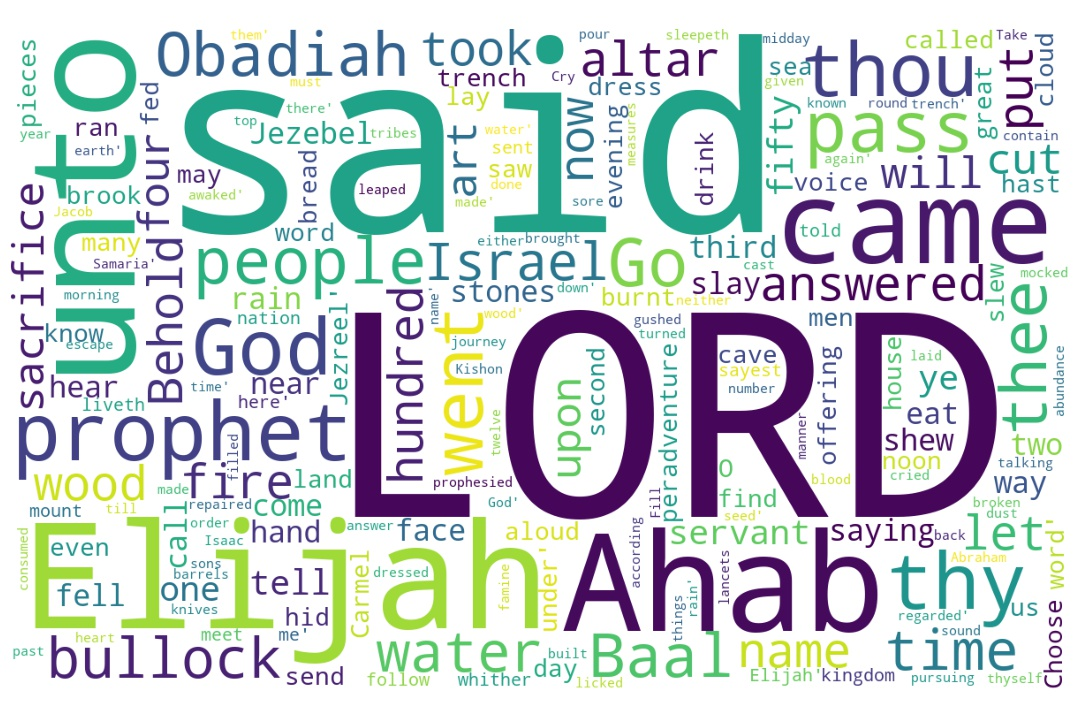
\includegraphics[width=\linewidth]{11OT-1Kings/1Kings18-WordCloud.jpg}
  \caption{1 Kings 18 Word Cloud}
  \label{fig:1 Kings 18 Word Cloud}
\end{figure}

%%%%%%%%%%%%%%%%%%%%%%%%%%%%%%%%%%%%%%%%%
%%%%%%%%%%%%%%%%%%%%%%%%%%%%%%%%%%%%%%%%%

\marginpar{\scriptsize \centering \fcolorbox{bone}{lime}{\textbf{ELIJAH AND THE BOYS OF BAAL}}\\ (1 Kings 18) \begin{compactenum}[I.][8]
    \item The \textbf{Forsaking} \index[scripture]{1Kings!1Ki 18:18} (1Ki 18:18) 
    \item The \textbf{Face-off} at Mt Carmel\index[scripture]{1Kings!1Ki 18:19} (1Ki 18:19) 
    \item The \textbf{False} Prophets \index[scripture]{1Kings!1Ki 18:22} (1Ki 18:22)  (450)
    \item The \textbf{Frenzy} \index[scripture]{1Kings!1Ki 18:26--29} (1Ki 18:26--29) 
    \item The \textbf{Failure} \index[scripture]{1Kings!1Ki 18:29} (1Ki 18:29) 
    \item The \textbf{Fire} of God \index[scripture]{1Kings!1Ki 18:38} (1Ki 18:38) 
    \item The \textbf{Finale} \index[scripture]{1Kings!1Ki 18:45} (1Ki 18:45) 
\end{compactenum}}


\footnote{\textcolor[cmyk]{0.99998,1,0,0}{\hyperlink{TOC}{Return to end of Table of Contents.}}}\footnote{\href{https://audiobible.com/bible/1_kings_18.html}{\textcolor[cmyk]{0.99998,1,0,0}{1 Kings 18 Audio}}}\textcolor[cmyk]{0.99998,1,0,0}{And \fcolorbox{bone}{bone}{it} came to pass \emph{after} many days, that the word of the LORD came to Elijah in the third year, saying, Go, shew thyself unto Ahab; and I will send rain upon the earth.}
[2] \textcolor[cmyk]{0.99998,1,0,0}{And Elijah went to shew himself unto Ahab. And \emph{there} \emph{was} a sore famine in Samaria.}
[3] \textcolor[cmyk]{0.99998,1,0,0}{And Ahab called Obadiah, which \emph{was} the governor of \emph{his} house. (Now Obadiah feared the LORD greatly:}
[4] \textcolor[cmyk]{0.99998,1,0,0}{For \fcolorbox{bone}{bone}{it} was \emph{so}, when Jezebel cut off the prophets of the LORD, that Obadiah took an hundred prophets, and hid them by fifty in a cave, and fed them with bread and water.)}
[5] \textcolor[cmyk]{0.99998,1,0,0}{And Ahab said unto Obadiah, Go into the land, unto all fountains of water, and unto all brooks: peradventure we may find grass to save the horses and mules alive, that we lose not all the beasts.}
[6] \textcolor[cmyk]{0.99998,1,0,0}{So \fcolorbox{bone}{bone}{they}  divided the land between them to pass throughout it: Ahab went one way by himself, and Obadiah went another way by himself.}\\
\\
\P  \textcolor[cmyk]{0.99998,1,0,0}{And as Obadiah was in the way, behold, Elijah met him: and he knew him, and fell on his face, and said, \emph{Art} thou that my lord Elijah?}
[8] \textcolor[cmyk]{0.99998,1,0,0}{And he answered him, I \emph{am}: go, tell thy lord, Behold, Elijah \emph{is} \emph{here}}
[9] \textcolor[cmyk]{0.99998,1,0,0}{And he said, What have I sinned, that thou wouldest deliver thy servant into the hand of Ahab, to slay me?}
[10] \textcolor[cmyk]{0.99998,1,0,0}{\emph{As} the LORD thy God liveth, there is no nation or kingdom, whither my lord hath not sent to seek thee: and when \fcolorbox{bone}{bone}{they}  said, \emph{He} \emph{is} not \emph{there}; he took an oath of the kingdom and nation, that \fcolorbox{bone}{bone}{they}  found thee not.}
[11] \textcolor[cmyk]{0.99998,1,0,0}{And now thou sayest, Go, tell thy lord, Behold, Elijah \emph{is} \emph{here}.}
[12] \textcolor[cmyk]{0.99998,1,0,0}{And \fcolorbox{bone}{bone}{it} shall come to pass, \emph{as} \emph{soon} \emph{as} I am gone from thee, that the Spirit of the LORD shall carry thee whither I know not; and \emph{so} when I come and tell Ahab, and he cannot find thee, he shall slay me: but I thy servant fear the LORD from my youth.}
[13] \textcolor[cmyk]{0.99998,1,0,0}{Was \fcolorbox{bone}{bone}{it} not told my lord what I did when Jezebel slew the prophets of the LORD, how I hid an hundred men of the LORD'S prophets by fifty in a cave, and fed them with bread and water?}
[14] \textcolor[cmyk]{0.99998,1,0,0}{And now thou sayest, Go, tell thy lord, Behold, Elijah \emph{is} \emph{here}: and he shall slay me.}
[15] \textcolor[cmyk]{0.99998,1,0,0}{And Elijah said, \emph{As} the LORD of hosts liveth, before whom I stand, I will surely shew myself unto him to day.}
[16] \textcolor[cmyk]{0.99998,1,0,0}{So Obadiah went to meet Ahab, and told him: and Ahab went to meet Elijah.}\\
\\
\P  \textcolor[cmyk]{0.99998,1,0,0}{And \fcolorbox{bone}{bone}{it} came to pass, when Ahab saw Elijah, that Ahab said unto him, \emph{Art} thou he that troubleth Israel?}
[18] \textcolor[cmyk]{0.99998,1,0,0}{And he answered, I have not troubled Israel; but thou, and thy father's house, in that ye have forsaken the commandments of the LORD, and thou hast followed Baalim.}
[19] \textcolor[cmyk]{0.99998,1,0,0}{Now therefore send, \emph{and} gather to me all Israel unto mount Carmel, and the prophets of Baal four hundred and fifty, and the prophets of the groves four hundred, which eat at Jezebel's table.}
[20] \textcolor[cmyk]{0.99998,1,0,0}{So Ahab sent unto all the children of Israel, and gathered the prophets together unto mount Carmel.}
[21] \textcolor[cmyk]{0.99998,1,0,0}{And Elijah came unto all the people, and said, How long halt ye between two opinions? if the LORD \emph{be} God, follow him: but if Baal, \emph{then} follow him. And the people answered him not a word.}
[22] \textcolor[cmyk]{0.99998,1,0,0}{Then said Elijah unto the people, I, \emph{even} I only, remain a prophet of the LORD; but Baal's prophets \emph{are} four hundred and fifty men.}
[23] \textcolor[cmyk]{0.99998,1,0,0}{Let them therefore give us two bullocks; and let them choose one bullock for themselves, and cut \fcolorbox{bone}{bone}{it} in pieces, and lay \emph{it} on wood, and put no fire \emph{under}: and I will dress the other bullock, and lay \emph{it} on wood, and put no fire \emph{under}:}
[24] \textcolor[cmyk]{0.99998,1,0,0}{And call ye on the name of your gods, and I will call on the name of the LORD: and the God that answereth by fire, let him be God. And all the people answered and said, \fcolorbox{bone}{bone}{it} is well spoken.}
[25] \textcolor[cmyk]{0.99998,1,0,0}{And Elijah said unto the prophets of Baal, Choose you one bullock for yourselves, and dress \emph{it} first; for ye \emph{are} many; and call on the name of your gods, but put no fire \emph{under}.}
[26] \textcolor[cmyk]{0.99998,1,0,0}{And \fcolorbox{bone}{bone}{they}  took the bullock which was given them, and \fcolorbox{bone}{bone}{they}  dressed \emph{it}, and called on the name of Baal from morning even until noon, saying, O Baal, hear us. But \emph{there} \emph{was} no voice, nor any that answered. And \fcolorbox{bone}{bone}{they}  leaped upon the altar which was made.}
[27] \textcolor[cmyk]{0.99998,1,0,0}{And \fcolorbox{bone}{bone}{it} came to pass at noon, that Elijah mocked them, and said, Cry aloud: for he \emph{is} a god; either he is talking, or he is pursuing, or he is in a journey, \emph{or} peradventure he sleepeth, and must be awaked.}
[28] \textcolor[cmyk]{0.99998,1,0,0}{And \fcolorbox{bone}{bone}{they}  cried aloud, and cut themselves after their manner with knives and lancets, till the blood gushed out upon them.}
[29] \textcolor[cmyk]{0.99998,1,0,0}{And \fcolorbox{bone}{bone}{it} came to pass, when midday was past, and \fcolorbox{bone}{bone}{they}  prophesied until the \emph{time} of the offering of the \emph{evening} sacrifice, that \emph{there} \emph{was} neither voice, nor any to answer, nor any that regarded.}
[30] \textcolor[cmyk]{0.99998,1,0,0}{And Elijah said unto all the people, Come near unto me. And all the people came near unto him. And he repaired the altar of the LORD \emph{that} \emph{was} broken down.}
[31] \textcolor[cmyk]{0.99998,1,0,0}{And Elijah took twelve stones, according to the number of the tribes of the sons of Jacob, unto whom the word of the LORD came, saying, Israel shall be thy name:}
[32] \textcolor[cmyk]{0.99998,1,0,0}{And with the stones he built an altar in the name of the LORD: and he made a trench about the altar, as great as would contain two measures of seed.}
[33] \textcolor[cmyk]{0.99998,1,0,0}{And he put the wood in order, and cut the bullock in pieces, and laid \emph{him} on the wood, and said, Fill four barrels with water, and pour \emph{it} on the burnt sacrifice, and on the wood.}
[34] \textcolor[cmyk]{0.99998,1,0,0}{And he said, Do \emph{it} the second time. And \fcolorbox{bone}{bone}{they}  did \emph{it} the second time. And he said, Do \emph{it} the third time. And \fcolorbox{bone}{bone}{they}  did \emph{it} the third time.}
[35] \textcolor[cmyk]{0.99998,1,0,0}{And the water ran round about the altar; and he filled the trench also with water.}
[36] \textcolor[cmyk]{0.99998,1,0,0}{And \fcolorbox{bone}{bone}{it} came to pass at \emph{the} \emph{time} \emph{of} the offering of the \emph{evening} sacrifice, that Elijah the prophet came near, and said, LORD God of Abraham, Isaac, and of Israel, let \fcolorbox{bone}{bone}{it} be known this day that thou \emph{art} God in Israel, and \emph{that} I \emph{am} thy servant, and \emph{that} I have done all these things at thy word.}
[37] \textcolor[cmyk]{0.99998,1,0,0}{Hear me, O LORD, hear me, that this people may know that thou \emph{art} the LORD God, and \emph{that} thou hast turned their heart back again.}
[38] \textcolor[cmyk]{0.99998,1,0,0}{Then the fire of the LORD fell, and consumed the burnt sacrifice, and the wood, and the stones, and the dust, and licked up the water that \emph{was} in the trench.}
[39] \textcolor[cmyk]{0.99998,1,0,0}{And when all the people saw \emph{it}, \fcolorbox{bone}{bone}{they}  fell on their faces: and \fcolorbox{bone}{bone}{they}  said, The LORD, he \emph{is} the God; the LORD, he \emph{is} the God.}
[40] \textcolor[cmyk]{0.99998,1,0,0}{And Elijah said unto them, Take the prophets of Baal; let not one of them escape. And \fcolorbox{bone}{bone}{they}  took them: and Elijah brought them down to the brook Kishon, and slew them there.}\\
\\
\P  \textcolor[cmyk]{0.99998,1,0,0}{And Elijah said unto Ahab, Get thee up, eat and drink; for \emph{there} \emph{is} a sound of abundance of rain.}
[42] \textcolor[cmyk]{0.99998,1,0,0}{So Ahab went up to eat and to drink. And Elijah went up to the top of Carmel; and he cast himself down upon the earth, and put his face between his knees,}
[43] \textcolor[cmyk]{0.99998,1,0,0}{And said to his servant, Go up now, look toward the sea. And he went up, and looked, and said, \emph{There} \emph{is} nothing. And he said, Go again seven times.}
[44] \textcolor[cmyk]{0.99998,1,0,0}{And \fcolorbox{bone}{bone}{it} came to pass at the seventh time, that he said, Behold, there ariseth a little cloud out of the sea, like a man's hand. And he said, Go up, say unto Ahab, Prepare \emph{thy} \emph{chariot}, and get thee down, that the rain stop thee not.}
[45] \textcolor[cmyk]{0.99998,1,0,0}{And \fcolorbox{bone}{bone}{it} came to pass in the mean while, that the heaven was black with clouds and wind, and there was a great rain. And Ahab rode, and went to Jezreel.}
[46] \textcolor[cmyk]{0.99998,1,0,0}{And the hand of the LORD was on Elijah; and he girded up his loins, and ran before Ahab to the entrance of Jezreel.}


\index[NWIV]{35!1Kings!1Ki 18:1}\index[AWIP]{And!1Kings!1Ki 18:1}\index[AWIP]{it!1Kings!1Ki 18:1}\index[AWIP]{came!1Kings!1Ki 18:1}\index[AWIP]{came!1Kings!1Ki 18:1 (2)}\index[AWIP]{to!1Kings!1Ki 18:1}\index[AWIP]{to!1Kings!1Ki 18:1 (2)}\index[AWIP]{pass!1Kings!1Ki 18:1}\index[AWIP]{\emph{after}!1Kings!1Ki 18:1}\index[AWIP]{many!1Kings!1Ki 18:1}\index[AWIP]{days!1Kings!1Ki 18:1}\index[AWIP]{that!1Kings!1Ki 18:1}\index[AWIP]{the!1Kings!1Ki 18:1}\index[AWIP]{the!1Kings!1Ki 18:1 (2)}\index[AWIP]{the!1Kings!1Ki 18:1 (3)}\index[AWIP]{the!1Kings!1Ki 18:1 (4)}\index[AWIP]{word!1Kings!1Ki 18:1}\index[AWIP]{of!1Kings!1Ki 18:1}\index[AWIP]{LORD!1Kings!1Ki 18:1}\index[AWIP]{Elijah!1Kings!1Ki 18:1}\index[AWIP]{in!1Kings!1Ki 18:1}\index[AWIP]{third!1Kings!1Ki 18:1}\index[AWIP]{year!1Kings!1Ki 18:1}\index[AWIP]{saying!1Kings!1Ki 18:1}\index[AWIP]{Go!1Kings!1Ki 18:1}\index[AWIP]{shew!1Kings!1Ki 18:1}\index[AWIP]{thyself!1Kings!1Ki 18:1}\index[AWIP]{unto!1Kings!1Ki 18:1}\index[AWIP]{Ahab!1Kings!1Ki 18:1}\index[AWIP]{and!1Kings!1Ki 18:1}\index[AWIP]{I!1Kings!1Ki 18:1}\index[AWIP]{will!1Kings!1Ki 18:1}\index[AWIP]{send!1Kings!1Ki 18:1}\index[AWIP]{rain!1Kings!1Ki 18:1}\index[AWIP]{upon!1Kings!1Ki 18:1}\index[AWIP]{earth!1Kings!1Ki 18:1}\index[AWIP]{\emph{after}!1Kings!1Ki 18:1}

\index[NWIV]{16!1Kings!1Ki 18:2}\index[AWIP]{And!1Kings!1Ki 18:2}\index[AWIP]{And!1Kings!1Ki 18:2 (2)}\index[AWIP]{Elijah!1Kings!1Ki 18:2}\index[AWIP]{went!1Kings!1Ki 18:2}\index[AWIP]{to!1Kings!1Ki 18:2}\index[AWIP]{shew!1Kings!1Ki 18:2}\index[AWIP]{himself!1Kings!1Ki 18:2}\index[AWIP]{unto!1Kings!1Ki 18:2}\index[AWIP]{Ahab!1Kings!1Ki 18:2}\index[AWIP]{\emph{there}!1Kings!1Ki 18:2}\index[AWIP]{\emph{was}!1Kings!1Ki 18:2}\index[AWIP]{a!1Kings!1Ki 18:2}\index[AWIP]{sore!1Kings!1Ki 18:2}\index[AWIP]{famine!1Kings!1Ki 18:2}\index[AWIP]{in!1Kings!1Ki 18:2}\index[AWIP]{Samaria!1Kings!1Ki 18:2}\index[AWIP]{\emph{there}!1Kings!1Ki 18:2}\index[AWIP]{\emph{was}!1Kings!1Ki 18:2}

\index[NWIV]{17!1Kings!1Ki 18:3}\index[AWIP]{And!1Kings!1Ki 18:3}\index[AWIP]{Ahab!1Kings!1Ki 18:3}\index[AWIP]{called!1Kings!1Ki 18:3}\index[AWIP]{Obadiah!1Kings!1Ki 18:3}\index[AWIP]{Obadiah!1Kings!1Ki 18:3 (2)}\index[AWIP]{which!1Kings!1Ki 18:3}\index[AWIP]{\emph{was}!1Kings!1Ki 18:3}\index[AWIP]{the!1Kings!1Ki 18:3}\index[AWIP]{the!1Kings!1Ki 18:3 (2)}\index[AWIP]{governor!1Kings!1Ki 18:3}\index[AWIP]{of!1Kings!1Ki 18:3}\index[AWIP]{\emph{his}!1Kings!1Ki 18:3}\index[AWIP]{house!1Kings!1Ki 18:3}\index[AWIP]{(Now!1Kings!1Ki 18:3}\index[AWIP]{feared!1Kings!1Ki 18:3}\index[AWIP]{LORD!1Kings!1Ki 18:3}\index[AWIP]{greatly!1Kings!1Ki 18:3}\index[AWIP]{\emph{was}!1Kings!1Ki 18:3}\index[AWIP]{\emph{his}!1Kings!1Ki 18:3}

\index[NWIV]{34!1Kings!1Ki 18:4}\index[AWIP]{For!1Kings!1Ki 18:4}\index[AWIP]{it!1Kings!1Ki 18:4}\index[AWIP]{was!1Kings!1Ki 18:4}\index[AWIP]{\emph{so}!1Kings!1Ki 18:4}\index[AWIP]{when!1Kings!1Ki 18:4}\index[AWIP]{Jezebel!1Kings!1Ki 18:4}\index[AWIP]{cut!1Kings!1Ki 18:4}\index[AWIP]{off!1Kings!1Ki 18:4}\index[AWIP]{the!1Kings!1Ki 18:4}\index[AWIP]{the!1Kings!1Ki 18:4 (2)}\index[AWIP]{prophets!1Kings!1Ki 18:4}\index[AWIP]{prophets!1Kings!1Ki 18:4 (2)}\index[AWIP]{of!1Kings!1Ki 18:4}\index[AWIP]{LORD!1Kings!1Ki 18:4}\index[AWIP]{that!1Kings!1Ki 18:4}\index[AWIP]{Obadiah!1Kings!1Ki 18:4}\index[AWIP]{took!1Kings!1Ki 18:4}\index[AWIP]{an!1Kings!1Ki 18:4}\index[AWIP]{hundred!1Kings!1Ki 18:4}\index[AWIP]{and!1Kings!1Ki 18:4}\index[AWIP]{and!1Kings!1Ki 18:4 (2)}\index[AWIP]{and!1Kings!1Ki 18:4 (3)}\index[AWIP]{hid!1Kings!1Ki 18:4}\index[AWIP]{them!1Kings!1Ki 18:4}\index[AWIP]{them!1Kings!1Ki 18:4 (2)}\index[AWIP]{by!1Kings!1Ki 18:4}\index[AWIP]{fifty!1Kings!1Ki 18:4}\index[AWIP]{in!1Kings!1Ki 18:4}\index[AWIP]{a!1Kings!1Ki 18:4}\index[AWIP]{cave!1Kings!1Ki 18:4}\index[AWIP]{fed!1Kings!1Ki 18:4}\index[AWIP]{with!1Kings!1Ki 18:4}\index[AWIP]{bread!1Kings!1Ki 18:4}\index[AWIP]{water)!1Kings!1Ki 18:4}\index[AWIP]{\emph{so}!1Kings!1Ki 18:4}

\index[NWIV]{37!1Kings!1Ki 18:5}\index[AWIP]{And!1Kings!1Ki 18:5}\index[AWIP]{Ahab!1Kings!1Ki 18:5}\index[AWIP]{said!1Kings!1Ki 18:5}\index[AWIP]{unto!1Kings!1Ki 18:5}\index[AWIP]{unto!1Kings!1Ki 18:5 (2)}\index[AWIP]{unto!1Kings!1Ki 18:5 (3)}\index[AWIP]{Obadiah!1Kings!1Ki 18:5}\index[AWIP]{Go!1Kings!1Ki 18:5}\index[AWIP]{into!1Kings!1Ki 18:5}\index[AWIP]{the!1Kings!1Ki 18:5}\index[AWIP]{the!1Kings!1Ki 18:5 (2)}\index[AWIP]{the!1Kings!1Ki 18:5 (3)}\index[AWIP]{land!1Kings!1Ki 18:5}\index[AWIP]{all!1Kings!1Ki 18:5}\index[AWIP]{all!1Kings!1Ki 18:5 (2)}\index[AWIP]{all!1Kings!1Ki 18:5 (3)}\index[AWIP]{fountains!1Kings!1Ki 18:5}\index[AWIP]{of!1Kings!1Ki 18:5}\index[AWIP]{water!1Kings!1Ki 18:5}\index[AWIP]{and!1Kings!1Ki 18:5}\index[AWIP]{and!1Kings!1Ki 18:5 (2)}\index[AWIP]{brooks!1Kings!1Ki 18:5}\index[AWIP]{peradventure!1Kings!1Ki 18:5}\index[AWIP]{we!1Kings!1Ki 18:5}\index[AWIP]{we!1Kings!1Ki 18:5 (2)}\index[AWIP]{may!1Kings!1Ki 18:5}\index[AWIP]{find!1Kings!1Ki 18:5}\index[AWIP]{grass!1Kings!1Ki 18:5}\index[AWIP]{to!1Kings!1Ki 18:5}\index[AWIP]{save!1Kings!1Ki 18:5}\index[AWIP]{horses!1Kings!1Ki 18:5}\index[AWIP]{mules!1Kings!1Ki 18:5}\index[AWIP]{alive!1Kings!1Ki 18:5}\index[AWIP]{that!1Kings!1Ki 18:5}\index[AWIP]{lose!1Kings!1Ki 18:5}\index[AWIP]{not!1Kings!1Ki 18:5}\index[AWIP]{beasts!1Kings!1Ki 18:5}

\index[NWIV]{24!1Kings!1Ki 18:6}\index[AWIP]{So!1Kings!1Ki 18:6}\index[AWIP]{they!1Kings!1Ki 18:6}\index[AWIP]{divided!1Kings!1Ki 18:6}\index[AWIP]{the!1Kings!1Ki 18:6}\index[AWIP]{land!1Kings!1Ki 18:6}\index[AWIP]{between!1Kings!1Ki 18:6}\index[AWIP]{them!1Kings!1Ki 18:6}\index[AWIP]{to!1Kings!1Ki 18:6}\index[AWIP]{pass!1Kings!1Ki 18:6}\index[AWIP]{throughout!1Kings!1Ki 18:6}\index[AWIP]{it!1Kings!1Ki 18:6}\index[AWIP]{Ahab!1Kings!1Ki 18:6}\index[AWIP]{went!1Kings!1Ki 18:6}\index[AWIP]{went!1Kings!1Ki 18:6 (2)}\index[AWIP]{one!1Kings!1Ki 18:6}\index[AWIP]{way!1Kings!1Ki 18:6}\index[AWIP]{way!1Kings!1Ki 18:6 (2)}\index[AWIP]{by!1Kings!1Ki 18:6}\index[AWIP]{by!1Kings!1Ki 18:6 (2)}\index[AWIP]{himself!1Kings!1Ki 18:6}\index[AWIP]{himself!1Kings!1Ki 18:6 (2)}\index[AWIP]{and!1Kings!1Ki 18:6}\index[AWIP]{Obadiah!1Kings!1Ki 18:6}\index[AWIP]{another!1Kings!1Ki 18:6}

\index[NWIV]{28!1Kings!1Ki 18:7}\index[AWIP]{And!1Kings!1Ki 18:7}\index[AWIP]{as!1Kings!1Ki 18:7}\index[AWIP]{Obadiah!1Kings!1Ki 18:7}\index[AWIP]{was!1Kings!1Ki 18:7}\index[AWIP]{in!1Kings!1Ki 18:7}\index[AWIP]{the!1Kings!1Ki 18:7}\index[AWIP]{way!1Kings!1Ki 18:7}\index[AWIP]{behold!1Kings!1Ki 18:7}\index[AWIP]{Elijah!1Kings!1Ki 18:7}\index[AWIP]{met!1Kings!1Ki 18:7}\index[AWIP]{him!1Kings!1Ki 18:7}\index[AWIP]{him!1Kings!1Ki 18:7 (2)}\index[AWIP]{and!1Kings!1Ki 18:7}\index[AWIP]{and!1Kings!1Ki 18:7 (2)}\index[AWIP]{and!1Kings!1Ki 18:7 (3)}\index[AWIP]{he!1Kings!1Ki 18:7}\index[AWIP]{knew!1Kings!1Ki 18:7}\index[AWIP]{fell!1Kings!1Ki 18:7}\index[AWIP]{on!1Kings!1Ki 18:7}\index[AWIP]{his!1Kings!1Ki 18:7}\index[AWIP]{face!1Kings!1Ki 18:7}\index[AWIP]{said!1Kings!1Ki 18:7}\index[AWIP]{\emph{Art}!1Kings!1Ki 18:7}\index[AWIP]{thou!1Kings!1Ki 18:7}\index[AWIP]{that!1Kings!1Ki 18:7}\index[AWIP]{my!1Kings!1Ki 18:7}\index[AWIP]{lord!1Kings!1Ki 18:7}\index[AWIP]{Elijah?!1Kings!1Ki 18:7}\index[AWIP]{\emph{Art}!1Kings!1Ki 18:7}

\index[NWIV]{14!1Kings!1Ki 18:8}\index[AWIP]{And!1Kings!1Ki 18:8}\index[AWIP]{he!1Kings!1Ki 18:8}\index[AWIP]{answered!1Kings!1Ki 18:8}\index[AWIP]{him!1Kings!1Ki 18:8}\index[AWIP]{I!1Kings!1Ki 18:8}\index[AWIP]{\emph{am}!1Kings!1Ki 18:8}\index[AWIP]{go!1Kings!1Ki 18:8}\index[AWIP]{tell!1Kings!1Ki 18:8}\index[AWIP]{thy!1Kings!1Ki 18:8}\index[AWIP]{lord!1Kings!1Ki 18:8}\index[AWIP]{Behold!1Kings!1Ki 18:8}\index[AWIP]{Elijah!1Kings!1Ki 18:8}\index[AWIP]{\emph{is}!1Kings!1Ki 18:8}\index[AWIP]{\emph{here}!1Kings!1Ki 18:8}\index[AWIP]{\emph{am}!1Kings!1Ki 18:8}\index[AWIP]{\emph{is}!1Kings!1Ki 18:8}\index[AWIP]{\emph{here}!1Kings!1Ki 18:8}

\index[NWIV]{21!1Kings!1Ki 18:9}\index[AWIP]{And!1Kings!1Ki 18:9}\index[AWIP]{he!1Kings!1Ki 18:9}\index[AWIP]{said!1Kings!1Ki 18:9}\index[AWIP]{What!1Kings!1Ki 18:9}\index[AWIP]{have!1Kings!1Ki 18:9}\index[AWIP]{I!1Kings!1Ki 18:9}\index[AWIP]{sinned!1Kings!1Ki 18:9}\index[AWIP]{that!1Kings!1Ki 18:9}\index[AWIP]{thou!1Kings!1Ki 18:9}\index[AWIP]{wouldest!1Kings!1Ki 18:9}\index[AWIP]{deliver!1Kings!1Ki 18:9}\index[AWIP]{thy!1Kings!1Ki 18:9}\index[AWIP]{servant!1Kings!1Ki 18:9}\index[AWIP]{into!1Kings!1Ki 18:9}\index[AWIP]{the!1Kings!1Ki 18:9}\index[AWIP]{hand!1Kings!1Ki 18:9}\index[AWIP]{of!1Kings!1Ki 18:9}\index[AWIP]{Ahab!1Kings!1Ki 18:9}\index[AWIP]{to!1Kings!1Ki 18:9}\index[AWIP]{slay!1Kings!1Ki 18:9}\index[AWIP]{me?!1Kings!1Ki 18:9}

\index[NWIV]{43!1Kings!1Ki 18:10}\index[AWIP]{\emph{As}!1Kings!1Ki 18:10}\index[AWIP]{the!1Kings!1Ki 18:10}\index[AWIP]{the!1Kings!1Ki 18:10 (2)}\index[AWIP]{LORD!1Kings!1Ki 18:10}\index[AWIP]{thy!1Kings!1Ki 18:10}\index[AWIP]{God!1Kings!1Ki 18:10}\index[AWIP]{liveth!1Kings!1Ki 18:10}\index[AWIP]{there!1Kings!1Ki 18:10}\index[AWIP]{is!1Kings!1Ki 18:10}\index[AWIP]{no!1Kings!1Ki 18:10}\index[AWIP]{nation!1Kings!1Ki 18:10}\index[AWIP]{nation!1Kings!1Ki 18:10 (2)}\index[AWIP]{or!1Kings!1Ki 18:10}\index[AWIP]{kingdom!1Kings!1Ki 18:10}\index[AWIP]{kingdom!1Kings!1Ki 18:10 (2)}\index[AWIP]{whither!1Kings!1Ki 18:10}\index[AWIP]{my!1Kings!1Ki 18:10}\index[AWIP]{lord!1Kings!1Ki 18:10}\index[AWIP]{hath!1Kings!1Ki 18:10}\index[AWIP]{not!1Kings!1Ki 18:10}\index[AWIP]{not!1Kings!1Ki 18:10 (2)}\index[AWIP]{not!1Kings!1Ki 18:10 (3)}\index[AWIP]{sent!1Kings!1Ki 18:10}\index[AWIP]{to!1Kings!1Ki 18:10}\index[AWIP]{seek!1Kings!1Ki 18:10}\index[AWIP]{thee!1Kings!1Ki 18:10}\index[AWIP]{thee!1Kings!1Ki 18:10 (2)}\index[AWIP]{and!1Kings!1Ki 18:10}\index[AWIP]{and!1Kings!1Ki 18:10 (2)}\index[AWIP]{when!1Kings!1Ki 18:10}\index[AWIP]{they!1Kings!1Ki 18:10}\index[AWIP]{they!1Kings!1Ki 18:10 (2)}\index[AWIP]{said!1Kings!1Ki 18:10}\index[AWIP]{\emph{He}!1Kings!1Ki 18:10}\index[AWIP]{\emph{is}!1Kings!1Ki 18:10}\index[AWIP]{\emph{there}!1Kings!1Ki 18:10}\index[AWIP]{he!1Kings!1Ki 18:10}\index[AWIP]{took!1Kings!1Ki 18:10}\index[AWIP]{an!1Kings!1Ki 18:10}\index[AWIP]{oath!1Kings!1Ki 18:10}\index[AWIP]{of!1Kings!1Ki 18:10}\index[AWIP]{that!1Kings!1Ki 18:10}\index[AWIP]{found!1Kings!1Ki 18:10}\index[AWIP]{\emph{As}!1Kings!1Ki 18:10}\index[AWIP]{\emph{He}!1Kings!1Ki 18:10}\index[AWIP]{\emph{is}!1Kings!1Ki 18:10}\index[AWIP]{\emph{there}!1Kings!1Ki 18:10}

\index[NWIV]{12!1Kings!1Ki 18:11}\index[AWIP]{And!1Kings!1Ki 18:11}\index[AWIP]{now!1Kings!1Ki 18:11}\index[AWIP]{thou!1Kings!1Ki 18:11}\index[AWIP]{sayest!1Kings!1Ki 18:11}\index[AWIP]{Go!1Kings!1Ki 18:11}\index[AWIP]{tell!1Kings!1Ki 18:11}\index[AWIP]{thy!1Kings!1Ki 18:11}\index[AWIP]{lord!1Kings!1Ki 18:11}\index[AWIP]{Behold!1Kings!1Ki 18:11}\index[AWIP]{Elijah!1Kings!1Ki 18:11}\index[AWIP]{\emph{is}!1Kings!1Ki 18:11}\index[AWIP]{\emph{here}!1Kings!1Ki 18:11}\index[AWIP]{\emph{is}!1Kings!1Ki 18:11}\index[AWIP]{\emph{here}!1Kings!1Ki 18:11}

\index[NWIV]{54!1Kings!1Ki 18:12}\index[AWIP]{And!1Kings!1Ki 18:12}\index[AWIP]{it!1Kings!1Ki 18:12}\index[AWIP]{shall!1Kings!1Ki 18:12}\index[AWIP]{shall!1Kings!1Ki 18:12 (2)}\index[AWIP]{shall!1Kings!1Ki 18:12 (3)}\index[AWIP]{come!1Kings!1Ki 18:12}\index[AWIP]{come!1Kings!1Ki 18:12 (2)}\index[AWIP]{to!1Kings!1Ki 18:12}\index[AWIP]{pass!1Kings!1Ki 18:12}\index[AWIP]{\emph{as}!1Kings!1Ki 18:12}\index[AWIP]{\emph{as}!1Kings!1Ki 18:12 (2)}\index[AWIP]{\emph{soon}!1Kings!1Ki 18:12}\index[AWIP]{I!1Kings!1Ki 18:12}\index[AWIP]{I!1Kings!1Ki 18:12 (2)}\index[AWIP]{I!1Kings!1Ki 18:12 (3)}\index[AWIP]{I!1Kings!1Ki 18:12 (4)}\index[AWIP]{am!1Kings!1Ki 18:12}\index[AWIP]{gone!1Kings!1Ki 18:12}\index[AWIP]{from!1Kings!1Ki 18:12}\index[AWIP]{from!1Kings!1Ki 18:12 (2)}\index[AWIP]{thee!1Kings!1Ki 18:12}\index[AWIP]{thee!1Kings!1Ki 18:12 (2)}\index[AWIP]{thee!1Kings!1Ki 18:12 (3)}\index[AWIP]{that!1Kings!1Ki 18:12}\index[AWIP]{the!1Kings!1Ki 18:12}\index[AWIP]{the!1Kings!1Ki 18:12 (2)}\index[AWIP]{the!1Kings!1Ki 18:12 (3)}\index[AWIP]{Spirit!1Kings!1Ki 18:12}\index[AWIP]{of!1Kings!1Ki 18:12}\index[AWIP]{LORD!1Kings!1Ki 18:12}\index[AWIP]{LORD!1Kings!1Ki 18:12 (2)}\index[AWIP]{carry!1Kings!1Ki 18:12}\index[AWIP]{whither!1Kings!1Ki 18:12}\index[AWIP]{know!1Kings!1Ki 18:12}\index[AWIP]{not!1Kings!1Ki 18:12}\index[AWIP]{and!1Kings!1Ki 18:12}\index[AWIP]{and!1Kings!1Ki 18:12 (2)}\index[AWIP]{and!1Kings!1Ki 18:12 (3)}\index[AWIP]{\emph{so}!1Kings!1Ki 18:12}\index[AWIP]{when!1Kings!1Ki 18:12}\index[AWIP]{tell!1Kings!1Ki 18:12}\index[AWIP]{Ahab!1Kings!1Ki 18:12}\index[AWIP]{he!1Kings!1Ki 18:12}\index[AWIP]{he!1Kings!1Ki 18:12 (2)}\index[AWIP]{cannot!1Kings!1Ki 18:12}\index[AWIP]{find!1Kings!1Ki 18:12}\index[AWIP]{slay!1Kings!1Ki 18:12}\index[AWIP]{me!1Kings!1Ki 18:12}\index[AWIP]{but!1Kings!1Ki 18:12}\index[AWIP]{thy!1Kings!1Ki 18:12}\index[AWIP]{servant!1Kings!1Ki 18:12}\index[AWIP]{fear!1Kings!1Ki 18:12}\index[AWIP]{my!1Kings!1Ki 18:12}\index[AWIP]{youth!1Kings!1Ki 18:12}\index[AWIP]{\emph{as}!1Kings!1Ki 18:12}\index[AWIP]{\emph{as}!1Kings!1Ki 18:12 (2)}\index[AWIP]{\emph{soon}!1Kings!1Ki 18:12}\index[AWIP]{\emph{so}!1Kings!1Ki 18:12}

\index[NWIV]{39!1Kings!1Ki 18:13}\index[AWIP]{Was!1Kings!1Ki 18:13}\index[AWIP]{it!1Kings!1Ki 18:13}\index[AWIP]{not!1Kings!1Ki 18:13}\index[AWIP]{told!1Kings!1Ki 18:13}\index[AWIP]{my!1Kings!1Ki 18:13}\index[AWIP]{lord!1Kings!1Ki 18:13}\index[AWIP]{what!1Kings!1Ki 18:13}\index[AWIP]{I!1Kings!1Ki 18:13}\index[AWIP]{I!1Kings!1Ki 18:13 (2)}\index[AWIP]{did!1Kings!1Ki 18:13}\index[AWIP]{when!1Kings!1Ki 18:13}\index[AWIP]{Jezebel!1Kings!1Ki 18:13}\index[AWIP]{slew!1Kings!1Ki 18:13}\index[AWIP]{the!1Kings!1Ki 18:13}\index[AWIP]{the!1Kings!1Ki 18:13 (2)}\index[AWIP]{the!1Kings!1Ki 18:13 (3)}\index[AWIP]{prophets!1Kings!1Ki 18:13}\index[AWIP]{prophets!1Kings!1Ki 18:13 (2)}\index[AWIP]{of!1Kings!1Ki 18:13}\index[AWIP]{of!1Kings!1Ki 18:13 (2)}\index[AWIP]{LORD!1Kings!1Ki 18:13}\index[AWIP]{how!1Kings!1Ki 18:13}\index[AWIP]{hid!1Kings!1Ki 18:13}\index[AWIP]{an!1Kings!1Ki 18:13}\index[AWIP]{hundred!1Kings!1Ki 18:13}\index[AWIP]{men!1Kings!1Ki 18:13}\index[AWIP]{LORD'S!1Kings!1Ki 18:13}\index[AWIP]{by!1Kings!1Ki 18:13}\index[AWIP]{fifty!1Kings!1Ki 18:13}\index[AWIP]{in!1Kings!1Ki 18:13}\index[AWIP]{a!1Kings!1Ki 18:13}\index[AWIP]{cave!1Kings!1Ki 18:13}\index[AWIP]{and!1Kings!1Ki 18:13}\index[AWIP]{and!1Kings!1Ki 18:13 (2)}\index[AWIP]{fed!1Kings!1Ki 18:13}\index[AWIP]{them!1Kings!1Ki 18:13}\index[AWIP]{with!1Kings!1Ki 18:13}\index[AWIP]{bread!1Kings!1Ki 18:13}\index[AWIP]{water?!1Kings!1Ki 18:13}

\index[NWIV]{17!1Kings!1Ki 18:14}\index[AWIP]{And!1Kings!1Ki 18:14}\index[AWIP]{now!1Kings!1Ki 18:14}\index[AWIP]{thou!1Kings!1Ki 18:14}\index[AWIP]{sayest!1Kings!1Ki 18:14}\index[AWIP]{Go!1Kings!1Ki 18:14}\index[AWIP]{tell!1Kings!1Ki 18:14}\index[AWIP]{thy!1Kings!1Ki 18:14}\index[AWIP]{lord!1Kings!1Ki 18:14}\index[AWIP]{Behold!1Kings!1Ki 18:14}\index[AWIP]{Elijah!1Kings!1Ki 18:14}\index[AWIP]{\emph{is}!1Kings!1Ki 18:14}\index[AWIP]{\emph{here}!1Kings!1Ki 18:14}\index[AWIP]{and!1Kings!1Ki 18:14}\index[AWIP]{he!1Kings!1Ki 18:14}\index[AWIP]{shall!1Kings!1Ki 18:14}\index[AWIP]{slay!1Kings!1Ki 18:14}\index[AWIP]{me!1Kings!1Ki 18:14}\index[AWIP]{\emph{is}!1Kings!1Ki 18:14}\index[AWIP]{\emph{here}!1Kings!1Ki 18:14}

\index[NWIV]{22!1Kings!1Ki 18:15}\index[AWIP]{And!1Kings!1Ki 18:15}\index[AWIP]{Elijah!1Kings!1Ki 18:15}\index[AWIP]{said!1Kings!1Ki 18:15}\index[AWIP]{\emph{As}!1Kings!1Ki 18:15}\index[AWIP]{the!1Kings!1Ki 18:15}\index[AWIP]{LORD!1Kings!1Ki 18:15}\index[AWIP]{of!1Kings!1Ki 18:15}\index[AWIP]{hosts!1Kings!1Ki 18:15}\index[AWIP]{liveth!1Kings!1Ki 18:15}\index[AWIP]{before!1Kings!1Ki 18:15}\index[AWIP]{whom!1Kings!1Ki 18:15}\index[AWIP]{I!1Kings!1Ki 18:15}\index[AWIP]{I!1Kings!1Ki 18:15 (2)}\index[AWIP]{stand!1Kings!1Ki 18:15}\index[AWIP]{will!1Kings!1Ki 18:15}\index[AWIP]{surely!1Kings!1Ki 18:15}\index[AWIP]{shew!1Kings!1Ki 18:15}\index[AWIP]{myself!1Kings!1Ki 18:15}\index[AWIP]{unto!1Kings!1Ki 18:15}\index[AWIP]{him!1Kings!1Ki 18:15}\index[AWIP]{to!1Kings!1Ki 18:15}\index[AWIP]{day!1Kings!1Ki 18:15}\index[AWIP]{\emph{As}!1Kings!1Ki 18:15}

\index[NWIV]{15!1Kings!1Ki 18:16}\index[AWIP]{So!1Kings!1Ki 18:16}\index[AWIP]{Obadiah!1Kings!1Ki 18:16}\index[AWIP]{went!1Kings!1Ki 18:16}\index[AWIP]{went!1Kings!1Ki 18:16 (2)}\index[AWIP]{to!1Kings!1Ki 18:16}\index[AWIP]{to!1Kings!1Ki 18:16 (2)}\index[AWIP]{meet!1Kings!1Ki 18:16}\index[AWIP]{meet!1Kings!1Ki 18:16 (2)}\index[AWIP]{Ahab!1Kings!1Ki 18:16}\index[AWIP]{Ahab!1Kings!1Ki 18:16 (2)}\index[AWIP]{and!1Kings!1Ki 18:16}\index[AWIP]{and!1Kings!1Ki 18:16 (2)}\index[AWIP]{told!1Kings!1Ki 18:16}\index[AWIP]{him!1Kings!1Ki 18:16}\index[AWIP]{Elijah!1Kings!1Ki 18:16}

\index[NWIV]{20!1Kings!1Ki 18:17}\index[AWIP]{And!1Kings!1Ki 18:17}\index[AWIP]{it!1Kings!1Ki 18:17}\index[AWIP]{came!1Kings!1Ki 18:17}\index[AWIP]{to!1Kings!1Ki 18:17}\index[AWIP]{pass!1Kings!1Ki 18:17}\index[AWIP]{when!1Kings!1Ki 18:17}\index[AWIP]{Ahab!1Kings!1Ki 18:17}\index[AWIP]{Ahab!1Kings!1Ki 18:17 (2)}\index[AWIP]{saw!1Kings!1Ki 18:17}\index[AWIP]{Elijah!1Kings!1Ki 18:17}\index[AWIP]{that!1Kings!1Ki 18:17}\index[AWIP]{that!1Kings!1Ki 18:17 (2)}\index[AWIP]{said!1Kings!1Ki 18:17}\index[AWIP]{unto!1Kings!1Ki 18:17}\index[AWIP]{him!1Kings!1Ki 18:17}\index[AWIP]{\emph{Art}!1Kings!1Ki 18:17}\index[AWIP]{thou!1Kings!1Ki 18:17}\index[AWIP]{he!1Kings!1Ki 18:17}\index[AWIP]{troubleth!1Kings!1Ki 18:17}\index[AWIP]{Israel?!1Kings!1Ki 18:17}\index[AWIP]{\emph{Art}!1Kings!1Ki 18:17}

\index[NWIV]{29!1Kings!1Ki 18:18}\index[AWIP]{And!1Kings!1Ki 18:18}\index[AWIP]{he!1Kings!1Ki 18:18}\index[AWIP]{answered!1Kings!1Ki 18:18}\index[AWIP]{I!1Kings!1Ki 18:18}\index[AWIP]{have!1Kings!1Ki 18:18}\index[AWIP]{have!1Kings!1Ki 18:18 (2)}\index[AWIP]{not!1Kings!1Ki 18:18}\index[AWIP]{troubled!1Kings!1Ki 18:18}\index[AWIP]{Israel!1Kings!1Ki 18:18}\index[AWIP]{but!1Kings!1Ki 18:18}\index[AWIP]{thou!1Kings!1Ki 18:18}\index[AWIP]{thou!1Kings!1Ki 18:18 (2)}\index[AWIP]{and!1Kings!1Ki 18:18}\index[AWIP]{and!1Kings!1Ki 18:18 (2)}\index[AWIP]{thy!1Kings!1Ki 18:18}\index[AWIP]{father's!1Kings!1Ki 18:18}\index[AWIP]{house!1Kings!1Ki 18:18}\index[AWIP]{in!1Kings!1Ki 18:18}\index[AWIP]{that!1Kings!1Ki 18:18}\index[AWIP]{ye!1Kings!1Ki 18:18}\index[AWIP]{forsaken!1Kings!1Ki 18:18}\index[AWIP]{the!1Kings!1Ki 18:18}\index[AWIP]{the!1Kings!1Ki 18:18 (2)}\index[AWIP]{commandments!1Kings!1Ki 18:18}\index[AWIP]{of!1Kings!1Ki 18:18}\index[AWIP]{LORD!1Kings!1Ki 18:18}\index[AWIP]{hast!1Kings!1Ki 18:18}\index[AWIP]{followed!1Kings!1Ki 18:18}\index[AWIP]{Baalim!1Kings!1Ki 18:18}

\index[NWIV]{34!1Kings!1Ki 18:19}\index[AWIP]{Now!1Kings!1Ki 18:19}\index[AWIP]{therefore!1Kings!1Ki 18:19}\index[AWIP]{send!1Kings!1Ki 18:19}\index[AWIP]{\emph{and}!1Kings!1Ki 18:19}\index[AWIP]{gather!1Kings!1Ki 18:19}\index[AWIP]{to!1Kings!1Ki 18:19}\index[AWIP]{me!1Kings!1Ki 18:19}\index[AWIP]{all!1Kings!1Ki 18:19}\index[AWIP]{Israel!1Kings!1Ki 18:19}\index[AWIP]{unto!1Kings!1Ki 18:19}\index[AWIP]{mount!1Kings!1Ki 18:19}\index[AWIP]{Carmel!1Kings!1Ki 18:19}\index[AWIP]{and!1Kings!1Ki 18:19}\index[AWIP]{and!1Kings!1Ki 18:19 (2)}\index[AWIP]{and!1Kings!1Ki 18:19 (3)}\index[AWIP]{the!1Kings!1Ki 18:19}\index[AWIP]{the!1Kings!1Ki 18:19 (2)}\index[AWIP]{the!1Kings!1Ki 18:19 (3)}\index[AWIP]{prophets!1Kings!1Ki 18:19}\index[AWIP]{prophets!1Kings!1Ki 18:19 (2)}\index[AWIP]{of!1Kings!1Ki 18:19}\index[AWIP]{of!1Kings!1Ki 18:19 (2)}\index[AWIP]{Baal!1Kings!1Ki 18:19}\index[AWIP]{four!1Kings!1Ki 18:19}\index[AWIP]{four!1Kings!1Ki 18:19 (2)}\index[AWIP]{hundred!1Kings!1Ki 18:19}\index[AWIP]{hundred!1Kings!1Ki 18:19 (2)}\index[AWIP]{fifty!1Kings!1Ki 18:19}\index[AWIP]{groves!1Kings!1Ki 18:19}\index[AWIP]{which!1Kings!1Ki 18:19}\index[AWIP]{eat!1Kings!1Ki 18:19}\index[AWIP]{at!1Kings!1Ki 18:19}\index[AWIP]{Jezebel's!1Kings!1Ki 18:19}\index[AWIP]{table!1Kings!1Ki 18:19}\index[AWIP]{\emph{and}!1Kings!1Ki 18:19}

\index[NWIV]{17!1Kings!1Ki 18:20}\index[AWIP]{So!1Kings!1Ki 18:20}\index[AWIP]{Ahab!1Kings!1Ki 18:20}\index[AWIP]{sent!1Kings!1Ki 18:20}\index[AWIP]{unto!1Kings!1Ki 18:20}\index[AWIP]{unto!1Kings!1Ki 18:20 (2)}\index[AWIP]{all!1Kings!1Ki 18:20}\index[AWIP]{the!1Kings!1Ki 18:20}\index[AWIP]{the!1Kings!1Ki 18:20 (2)}\index[AWIP]{children!1Kings!1Ki 18:20}\index[AWIP]{of!1Kings!1Ki 18:20}\index[AWIP]{Israel!1Kings!1Ki 18:20}\index[AWIP]{and!1Kings!1Ki 18:20}\index[AWIP]{gathered!1Kings!1Ki 18:20}\index[AWIP]{prophets!1Kings!1Ki 18:20}\index[AWIP]{together!1Kings!1Ki 18:20}\index[AWIP]{mount!1Kings!1Ki 18:20}\index[AWIP]{Carmel!1Kings!1Ki 18:20}

\index[NWIV]{37!1Kings!1Ki 18:21}\index[AWIP]{And!1Kings!1Ki 18:21}\index[AWIP]{And!1Kings!1Ki 18:21 (2)}\index[AWIP]{Elijah!1Kings!1Ki 18:21}\index[AWIP]{came!1Kings!1Ki 18:21}\index[AWIP]{unto!1Kings!1Ki 18:21}\index[AWIP]{all!1Kings!1Ki 18:21}\index[AWIP]{the!1Kings!1Ki 18:21}\index[AWIP]{the!1Kings!1Ki 18:21 (2)}\index[AWIP]{the!1Kings!1Ki 18:21 (3)}\index[AWIP]{people!1Kings!1Ki 18:21}\index[AWIP]{people!1Kings!1Ki 18:21 (2)}\index[AWIP]{and!1Kings!1Ki 18:21}\index[AWIP]{said!1Kings!1Ki 18:21}\index[AWIP]{How!1Kings!1Ki 18:21}\index[AWIP]{long!1Kings!1Ki 18:21}\index[AWIP]{halt!1Kings!1Ki 18:21}\index[AWIP]{ye!1Kings!1Ki 18:21}\index[AWIP]{between!1Kings!1Ki 18:21}\index[AWIP]{two!1Kings!1Ki 18:21}\index[AWIP]{opinions?!1Kings!1Ki 18:21}\index[AWIP]{if!1Kings!1Ki 18:21}\index[AWIP]{if!1Kings!1Ki 18:21 (2)}\index[AWIP]{LORD!1Kings!1Ki 18:21}\index[AWIP]{\emph{be}!1Kings!1Ki 18:21}\index[AWIP]{God!1Kings!1Ki 18:21}\index[AWIP]{follow!1Kings!1Ki 18:21}\index[AWIP]{follow!1Kings!1Ki 18:21 (2)}\index[AWIP]{him!1Kings!1Ki 18:21}\index[AWIP]{him!1Kings!1Ki 18:21 (2)}\index[AWIP]{him!1Kings!1Ki 18:21 (3)}\index[AWIP]{but!1Kings!1Ki 18:21}\index[AWIP]{Baal!1Kings!1Ki 18:21}\index[AWIP]{\emph{then}!1Kings!1Ki 18:21}\index[AWIP]{answered!1Kings!1Ki 18:21}\index[AWIP]{not!1Kings!1Ki 18:21}\index[AWIP]{a!1Kings!1Ki 18:21}\index[AWIP]{word!1Kings!1Ki 18:21}\index[AWIP]{\emph{be}!1Kings!1Ki 18:21}\index[AWIP]{\emph{then}!1Kings!1Ki 18:21}

\index[NWIV]{25!1Kings!1Ki 18:22}\index[AWIP]{Then!1Kings!1Ki 18:22}\index[AWIP]{said!1Kings!1Ki 18:22}\index[AWIP]{Elijah!1Kings!1Ki 18:22}\index[AWIP]{unto!1Kings!1Ki 18:22}\index[AWIP]{the!1Kings!1Ki 18:22}\index[AWIP]{the!1Kings!1Ki 18:22 (2)}\index[AWIP]{people!1Kings!1Ki 18:22}\index[AWIP]{I!1Kings!1Ki 18:22}\index[AWIP]{I!1Kings!1Ki 18:22 (2)}\index[AWIP]{\emph{even}!1Kings!1Ki 18:22}\index[AWIP]{only!1Kings!1Ki 18:22}\index[AWIP]{remain!1Kings!1Ki 18:22}\index[AWIP]{a!1Kings!1Ki 18:22}\index[AWIP]{prophet!1Kings!1Ki 18:22}\index[AWIP]{of!1Kings!1Ki 18:22}\index[AWIP]{LORD!1Kings!1Ki 18:22}\index[AWIP]{but!1Kings!1Ki 18:22}\index[AWIP]{Baal's!1Kings!1Ki 18:22}\index[AWIP]{prophets!1Kings!1Ki 18:22}\index[AWIP]{\emph{are}!1Kings!1Ki 18:22}\index[AWIP]{four!1Kings!1Ki 18:22}\index[AWIP]{hundred!1Kings!1Ki 18:22}\index[AWIP]{and!1Kings!1Ki 18:22}\index[AWIP]{fifty!1Kings!1Ki 18:22}\index[AWIP]{men!1Kings!1Ki 18:22}\index[AWIP]{\emph{even}!1Kings!1Ki 18:22}\index[AWIP]{\emph{are}!1Kings!1Ki 18:22}

\index[NWIV]{47!1Kings!1Ki 18:23}\index[AWIP]{Let!1Kings!1Ki 18:23}\index[AWIP]{them!1Kings!1Ki 18:23}\index[AWIP]{them!1Kings!1Ki 18:23 (2)}\index[AWIP]{therefore!1Kings!1Ki 18:23}\index[AWIP]{give!1Kings!1Ki 18:23}\index[AWIP]{us!1Kings!1Ki 18:23}\index[AWIP]{two!1Kings!1Ki 18:23}\index[AWIP]{bullocks!1Kings!1Ki 18:23}\index[AWIP]{and!1Kings!1Ki 18:23}\index[AWIP]{and!1Kings!1Ki 18:23 (2)}\index[AWIP]{and!1Kings!1Ki 18:23 (3)}\index[AWIP]{and!1Kings!1Ki 18:23 (4)}\index[AWIP]{and!1Kings!1Ki 18:23 (5)}\index[AWIP]{and!1Kings!1Ki 18:23 (6)}\index[AWIP]{and!1Kings!1Ki 18:23 (7)}\index[AWIP]{let!1Kings!1Ki 18:23}\index[AWIP]{choose!1Kings!1Ki 18:23}\index[AWIP]{one!1Kings!1Ki 18:23}\index[AWIP]{bullock!1Kings!1Ki 18:23}\index[AWIP]{bullock!1Kings!1Ki 18:23 (2)}\index[AWIP]{for!1Kings!1Ki 18:23}\index[AWIP]{themselves!1Kings!1Ki 18:23}\index[AWIP]{cut!1Kings!1Ki 18:23}\index[AWIP]{it!1Kings!1Ki 18:23}\index[AWIP]{in!1Kings!1Ki 18:23}\index[AWIP]{pieces!1Kings!1Ki 18:23}\index[AWIP]{lay!1Kings!1Ki 18:23}\index[AWIP]{lay!1Kings!1Ki 18:23 (2)}\index[AWIP]{\emph{it}!1Kings!1Ki 18:23}\index[AWIP]{\emph{it}!1Kings!1Ki 18:23 (2)}\index[AWIP]{on!1Kings!1Ki 18:23}\index[AWIP]{on!1Kings!1Ki 18:23 (2)}\index[AWIP]{wood!1Kings!1Ki 18:23}\index[AWIP]{wood!1Kings!1Ki 18:23 (2)}\index[AWIP]{put!1Kings!1Ki 18:23}\index[AWIP]{put!1Kings!1Ki 18:23 (2)}\index[AWIP]{no!1Kings!1Ki 18:23}\index[AWIP]{no!1Kings!1Ki 18:23 (2)}\index[AWIP]{fire!1Kings!1Ki 18:23}\index[AWIP]{fire!1Kings!1Ki 18:23 (2)}\index[AWIP]{\emph{under}!1Kings!1Ki 18:23}\index[AWIP]{\emph{under}!1Kings!1Ki 18:23 (2)}\index[AWIP]{I!1Kings!1Ki 18:23}\index[AWIP]{will!1Kings!1Ki 18:23}\index[AWIP]{dress!1Kings!1Ki 18:23}\index[AWIP]{the!1Kings!1Ki 18:23}\index[AWIP]{other!1Kings!1Ki 18:23}\index[AWIP]{\emph{it}!1Kings!1Ki 18:23}\index[AWIP]{\emph{it}!1Kings!1Ki 18:23 (2)}\index[AWIP]{\emph{under}!1Kings!1Ki 18:23}\index[AWIP]{\emph{under}!1Kings!1Ki 18:23 (2)}

\index[NWIV]{41!1Kings!1Ki 18:24}\index[AWIP]{And!1Kings!1Ki 18:24}\index[AWIP]{And!1Kings!1Ki 18:24 (2)}\index[AWIP]{call!1Kings!1Ki 18:24}\index[AWIP]{call!1Kings!1Ki 18:24 (2)}\index[AWIP]{ye!1Kings!1Ki 18:24}\index[AWIP]{on!1Kings!1Ki 18:24}\index[AWIP]{on!1Kings!1Ki 18:24 (2)}\index[AWIP]{the!1Kings!1Ki 18:24}\index[AWIP]{the!1Kings!1Ki 18:24 (2)}\index[AWIP]{the!1Kings!1Ki 18:24 (3)}\index[AWIP]{the!1Kings!1Ki 18:24 (4)}\index[AWIP]{the!1Kings!1Ki 18:24 (5)}\index[AWIP]{name!1Kings!1Ki 18:24}\index[AWIP]{name!1Kings!1Ki 18:24 (2)}\index[AWIP]{of!1Kings!1Ki 18:24}\index[AWIP]{of!1Kings!1Ki 18:24 (2)}\index[AWIP]{your!1Kings!1Ki 18:24}\index[AWIP]{gods!1Kings!1Ki 18:24}\index[AWIP]{and!1Kings!1Ki 18:24}\index[AWIP]{and!1Kings!1Ki 18:24 (2)}\index[AWIP]{and!1Kings!1Ki 18:24 (3)}\index[AWIP]{I!1Kings!1Ki 18:24}\index[AWIP]{will!1Kings!1Ki 18:24}\index[AWIP]{LORD!1Kings!1Ki 18:24}\index[AWIP]{God!1Kings!1Ki 18:24}\index[AWIP]{God!1Kings!1Ki 18:24 (2)}\index[AWIP]{that!1Kings!1Ki 18:24}\index[AWIP]{answereth!1Kings!1Ki 18:24}\index[AWIP]{by!1Kings!1Ki 18:24}\index[AWIP]{fire!1Kings!1Ki 18:24}\index[AWIP]{let!1Kings!1Ki 18:24}\index[AWIP]{him!1Kings!1Ki 18:24}\index[AWIP]{be!1Kings!1Ki 18:24}\index[AWIP]{all!1Kings!1Ki 18:24}\index[AWIP]{people!1Kings!1Ki 18:24}\index[AWIP]{answered!1Kings!1Ki 18:24}\index[AWIP]{said!1Kings!1Ki 18:24}\index[AWIP]{It!1Kings!1Ki 18:24}\index[AWIP]{is!1Kings!1Ki 18:24}\index[AWIP]{well!1Kings!1Ki 18:24}\index[AWIP]{spoken!1Kings!1Ki 18:24}

\index[NWIV]{35!1Kings!1Ki 18:25}\index[AWIP]{And!1Kings!1Ki 18:25}\index[AWIP]{Elijah!1Kings!1Ki 18:25}\index[AWIP]{said!1Kings!1Ki 18:25}\index[AWIP]{unto!1Kings!1Ki 18:25}\index[AWIP]{the!1Kings!1Ki 18:25}\index[AWIP]{the!1Kings!1Ki 18:25 (2)}\index[AWIP]{prophets!1Kings!1Ki 18:25}\index[AWIP]{of!1Kings!1Ki 18:25}\index[AWIP]{of!1Kings!1Ki 18:25 (2)}\index[AWIP]{Baal!1Kings!1Ki 18:25}\index[AWIP]{Choose!1Kings!1Ki 18:25}\index[AWIP]{you!1Kings!1Ki 18:25}\index[AWIP]{one!1Kings!1Ki 18:25}\index[AWIP]{bullock!1Kings!1Ki 18:25}\index[AWIP]{for!1Kings!1Ki 18:25}\index[AWIP]{for!1Kings!1Ki 18:25 (2)}\index[AWIP]{yourselves!1Kings!1Ki 18:25}\index[AWIP]{and!1Kings!1Ki 18:25}\index[AWIP]{and!1Kings!1Ki 18:25 (2)}\index[AWIP]{dress!1Kings!1Ki 18:25}\index[AWIP]{\emph{it}!1Kings!1Ki 18:25}\index[AWIP]{first!1Kings!1Ki 18:25}\index[AWIP]{ye!1Kings!1Ki 18:25}\index[AWIP]{\emph{are}!1Kings!1Ki 18:25}\index[AWIP]{many!1Kings!1Ki 18:25}\index[AWIP]{call!1Kings!1Ki 18:25}\index[AWIP]{on!1Kings!1Ki 18:25}\index[AWIP]{name!1Kings!1Ki 18:25}\index[AWIP]{your!1Kings!1Ki 18:25}\index[AWIP]{gods!1Kings!1Ki 18:25}\index[AWIP]{but!1Kings!1Ki 18:25}\index[AWIP]{put!1Kings!1Ki 18:25}\index[AWIP]{no!1Kings!1Ki 18:25}\index[AWIP]{fire!1Kings!1Ki 18:25}\index[AWIP]{\emph{under}!1Kings!1Ki 18:25}\index[AWIP]{\emph{it}!1Kings!1Ki 18:25}\index[AWIP]{\emph{are}!1Kings!1Ki 18:25}\index[AWIP]{\emph{under}!1Kings!1Ki 18:25}

\index[NWIV]{48!1Kings!1Ki 18:26}\index[AWIP]{And!1Kings!1Ki 18:26}\index[AWIP]{And!1Kings!1Ki 18:26 (2)}\index[AWIP]{they!1Kings!1Ki 18:26}\index[AWIP]{they!1Kings!1Ki 18:26 (2)}\index[AWIP]{they!1Kings!1Ki 18:26 (3)}\index[AWIP]{took!1Kings!1Ki 18:26}\index[AWIP]{the!1Kings!1Ki 18:26}\index[AWIP]{the!1Kings!1Ki 18:26 (2)}\index[AWIP]{the!1Kings!1Ki 18:26 (3)}\index[AWIP]{bullock!1Kings!1Ki 18:26}\index[AWIP]{which!1Kings!1Ki 18:26}\index[AWIP]{which!1Kings!1Ki 18:26 (2)}\index[AWIP]{was!1Kings!1Ki 18:26}\index[AWIP]{was!1Kings!1Ki 18:26 (2)}\index[AWIP]{given!1Kings!1Ki 18:26}\index[AWIP]{them!1Kings!1Ki 18:26}\index[AWIP]{and!1Kings!1Ki 18:26}\index[AWIP]{and!1Kings!1Ki 18:26 (2)}\index[AWIP]{dressed!1Kings!1Ki 18:26}\index[AWIP]{\emph{it}!1Kings!1Ki 18:26}\index[AWIP]{called!1Kings!1Ki 18:26}\index[AWIP]{on!1Kings!1Ki 18:26}\index[AWIP]{name!1Kings!1Ki 18:26}\index[AWIP]{of!1Kings!1Ki 18:26}\index[AWIP]{Baal!1Kings!1Ki 18:26}\index[AWIP]{Baal!1Kings!1Ki 18:26 (2)}\index[AWIP]{from!1Kings!1Ki 18:26}\index[AWIP]{morning!1Kings!1Ki 18:26}\index[AWIP]{even!1Kings!1Ki 18:26}\index[AWIP]{until!1Kings!1Ki 18:26}\index[AWIP]{noon!1Kings!1Ki 18:26}\index[AWIP]{saying!1Kings!1Ki 18:26}\index[AWIP]{O!1Kings!1Ki 18:26}\index[AWIP]{hear!1Kings!1Ki 18:26}\index[AWIP]{us!1Kings!1Ki 18:26}\index[AWIP]{But!1Kings!1Ki 18:26}\index[AWIP]{\emph{there}!1Kings!1Ki 18:26}\index[AWIP]{\emph{was}!1Kings!1Ki 18:26}\index[AWIP]{no!1Kings!1Ki 18:26}\index[AWIP]{voice!1Kings!1Ki 18:26}\index[AWIP]{nor!1Kings!1Ki 18:26}\index[AWIP]{any!1Kings!1Ki 18:26}\index[AWIP]{that!1Kings!1Ki 18:26}\index[AWIP]{answered!1Kings!1Ki 18:26}\index[AWIP]{leaped!1Kings!1Ki 18:26}\index[AWIP]{upon!1Kings!1Ki 18:26}\index[AWIP]{altar!1Kings!1Ki 18:26}\index[AWIP]{made!1Kings!1Ki 18:26}\index[AWIP]{\emph{it}!1Kings!1Ki 18:26}\index[AWIP]{\emph{there}!1Kings!1Ki 18:26}\index[AWIP]{\emph{was}!1Kings!1Ki 18:26}

\index[NWIV]{42!1Kings!1Ki 18:27}\index[AWIP]{And!1Kings!1Ki 18:27}\index[AWIP]{it!1Kings!1Ki 18:27}\index[AWIP]{came!1Kings!1Ki 18:27}\index[AWIP]{to!1Kings!1Ki 18:27}\index[AWIP]{pass!1Kings!1Ki 18:27}\index[AWIP]{at!1Kings!1Ki 18:27}\index[AWIP]{noon!1Kings!1Ki 18:27}\index[AWIP]{that!1Kings!1Ki 18:27}\index[AWIP]{Elijah!1Kings!1Ki 18:27}\index[AWIP]{mocked!1Kings!1Ki 18:27}\index[AWIP]{them!1Kings!1Ki 18:27}\index[AWIP]{and!1Kings!1Ki 18:27}\index[AWIP]{and!1Kings!1Ki 18:27 (2)}\index[AWIP]{said!1Kings!1Ki 18:27}\index[AWIP]{Cry!1Kings!1Ki 18:27}\index[AWIP]{aloud!1Kings!1Ki 18:27}\index[AWIP]{for!1Kings!1Ki 18:27}\index[AWIP]{he!1Kings!1Ki 18:27}\index[AWIP]{he!1Kings!1Ki 18:27 (2)}\index[AWIP]{he!1Kings!1Ki 18:27 (3)}\index[AWIP]{he!1Kings!1Ki 18:27 (4)}\index[AWIP]{he!1Kings!1Ki 18:27 (5)}\index[AWIP]{\emph{is}!1Kings!1Ki 18:27}\index[AWIP]{a!1Kings!1Ki 18:27}\index[AWIP]{a!1Kings!1Ki 18:27 (2)}\index[AWIP]{god!1Kings!1Ki 18:27}\index[AWIP]{either!1Kings!1Ki 18:27}\index[AWIP]{is!1Kings!1Ki 18:27}\index[AWIP]{is!1Kings!1Ki 18:27 (2)}\index[AWIP]{is!1Kings!1Ki 18:27 (3)}\index[AWIP]{talking!1Kings!1Ki 18:27}\index[AWIP]{or!1Kings!1Ki 18:27}\index[AWIP]{or!1Kings!1Ki 18:27 (2)}\index[AWIP]{pursuing!1Kings!1Ki 18:27}\index[AWIP]{in!1Kings!1Ki 18:27}\index[AWIP]{journey!1Kings!1Ki 18:27}\index[AWIP]{\emph{or}!1Kings!1Ki 18:27}\index[AWIP]{peradventure!1Kings!1Ki 18:27}\index[AWIP]{sleepeth!1Kings!1Ki 18:27}\index[AWIP]{must!1Kings!1Ki 18:27}\index[AWIP]{be!1Kings!1Ki 18:27}\index[AWIP]{awaked!1Kings!1Ki 18:27}\index[AWIP]{\emph{is}!1Kings!1Ki 18:27}\index[AWIP]{\emph{or}!1Kings!1Ki 18:27}

\index[NWIV]{21!1Kings!1Ki 18:28}\index[AWIP]{And!1Kings!1Ki 18:28}\index[AWIP]{they!1Kings!1Ki 18:28}\index[AWIP]{cried!1Kings!1Ki 18:28}\index[AWIP]{aloud!1Kings!1Ki 18:28}\index[AWIP]{and!1Kings!1Ki 18:28}\index[AWIP]{and!1Kings!1Ki 18:28 (2)}\index[AWIP]{cut!1Kings!1Ki 18:28}\index[AWIP]{themselves!1Kings!1Ki 18:28}\index[AWIP]{after!1Kings!1Ki 18:28}\index[AWIP]{their!1Kings!1Ki 18:28}\index[AWIP]{manner!1Kings!1Ki 18:28}\index[AWIP]{with!1Kings!1Ki 18:28}\index[AWIP]{knives!1Kings!1Ki 18:28}\index[AWIP]{lancets!1Kings!1Ki 18:28}\index[AWIP]{till!1Kings!1Ki 18:28}\index[AWIP]{the!1Kings!1Ki 18:28}\index[AWIP]{blood!1Kings!1Ki 18:28}\index[AWIP]{gushed!1Kings!1Ki 18:28}\index[AWIP]{out!1Kings!1Ki 18:28}\index[AWIP]{upon!1Kings!1Ki 18:28}\index[AWIP]{them!1Kings!1Ki 18:28}

\index[NWIV]{35!1Kings!1Ki 18:29}\index[AWIP]{And!1Kings!1Ki 18:29}\index[AWIP]{it!1Kings!1Ki 18:29}\index[AWIP]{came!1Kings!1Ki 18:29}\index[AWIP]{to!1Kings!1Ki 18:29}\index[AWIP]{to!1Kings!1Ki 18:29 (2)}\index[AWIP]{pass!1Kings!1Ki 18:29}\index[AWIP]{when!1Kings!1Ki 18:29}\index[AWIP]{midday!1Kings!1Ki 18:29}\index[AWIP]{was!1Kings!1Ki 18:29}\index[AWIP]{past!1Kings!1Ki 18:29}\index[AWIP]{and!1Kings!1Ki 18:29}\index[AWIP]{they!1Kings!1Ki 18:29}\index[AWIP]{prophesied!1Kings!1Ki 18:29}\index[AWIP]{until!1Kings!1Ki 18:29}\index[AWIP]{the!1Kings!1Ki 18:29}\index[AWIP]{the!1Kings!1Ki 18:29 (2)}\index[AWIP]{the!1Kings!1Ki 18:29 (3)}\index[AWIP]{\emph{time}!1Kings!1Ki 18:29}\index[AWIP]{of!1Kings!1Ki 18:29}\index[AWIP]{of!1Kings!1Ki 18:29 (2)}\index[AWIP]{offering!1Kings!1Ki 18:29}\index[AWIP]{\emph{evening}!1Kings!1Ki 18:29}\index[AWIP]{sacrifice!1Kings!1Ki 18:29}\index[AWIP]{that!1Kings!1Ki 18:29}\index[AWIP]{that!1Kings!1Ki 18:29 (2)}\index[AWIP]{\emph{there}!1Kings!1Ki 18:29}\index[AWIP]{\emph{was}!1Kings!1Ki 18:29}\index[AWIP]{neither!1Kings!1Ki 18:29}\index[AWIP]{voice!1Kings!1Ki 18:29}\index[AWIP]{nor!1Kings!1Ki 18:29}\index[AWIP]{nor!1Kings!1Ki 18:29 (2)}\index[AWIP]{any!1Kings!1Ki 18:29}\index[AWIP]{any!1Kings!1Ki 18:29 (2)}\index[AWIP]{answer!1Kings!1Ki 18:29}\index[AWIP]{regarded!1Kings!1Ki 18:29}\index[AWIP]{\emph{time}!1Kings!1Ki 18:29}\index[AWIP]{\emph{evening}!1Kings!1Ki 18:29}\index[AWIP]{\emph{there}!1Kings!1Ki 18:29}\index[AWIP]{\emph{was}!1Kings!1Ki 18:29}

\index[NWIV]{31!1Kings!1Ki 18:30}\index[AWIP]{And!1Kings!1Ki 18:30}\index[AWIP]{And!1Kings!1Ki 18:30 (2)}\index[AWIP]{And!1Kings!1Ki 18:30 (3)}\index[AWIP]{Elijah!1Kings!1Ki 18:30}\index[AWIP]{said!1Kings!1Ki 18:30}\index[AWIP]{unto!1Kings!1Ki 18:30}\index[AWIP]{unto!1Kings!1Ki 18:30 (2)}\index[AWIP]{unto!1Kings!1Ki 18:30 (3)}\index[AWIP]{all!1Kings!1Ki 18:30}\index[AWIP]{all!1Kings!1Ki 18:30 (2)}\index[AWIP]{the!1Kings!1Ki 18:30}\index[AWIP]{the!1Kings!1Ki 18:30 (2)}\index[AWIP]{the!1Kings!1Ki 18:30 (3)}\index[AWIP]{the!1Kings!1Ki 18:30 (4)}\index[AWIP]{people!1Kings!1Ki 18:30}\index[AWIP]{people!1Kings!1Ki 18:30 (2)}\index[AWIP]{Come!1Kings!1Ki 18:30}\index[AWIP]{near!1Kings!1Ki 18:30}\index[AWIP]{near!1Kings!1Ki 18:30 (2)}\index[AWIP]{me!1Kings!1Ki 18:30}\index[AWIP]{came!1Kings!1Ki 18:30}\index[AWIP]{him!1Kings!1Ki 18:30}\index[AWIP]{he!1Kings!1Ki 18:30}\index[AWIP]{repaired!1Kings!1Ki 18:30}\index[AWIP]{altar!1Kings!1Ki 18:30}\index[AWIP]{of!1Kings!1Ki 18:30}\index[AWIP]{LORD!1Kings!1Ki 18:30}\index[AWIP]{\emph{that}!1Kings!1Ki 18:30}\index[AWIP]{\emph{was}!1Kings!1Ki 18:30}\index[AWIP]{broken!1Kings!1Ki 18:30}\index[AWIP]{down!1Kings!1Ki 18:30}\index[AWIP]{\emph{that}!1Kings!1Ki 18:30}\index[AWIP]{\emph{was}!1Kings!1Ki 18:30}

\index[NWIV]{31!1Kings!1Ki 18:31}\index[AWIP]{And!1Kings!1Ki 18:31}\index[AWIP]{Elijah!1Kings!1Ki 18:31}\index[AWIP]{took!1Kings!1Ki 18:31}\index[AWIP]{twelve!1Kings!1Ki 18:31}\index[AWIP]{stones!1Kings!1Ki 18:31}\index[AWIP]{according!1Kings!1Ki 18:31}\index[AWIP]{to!1Kings!1Ki 18:31}\index[AWIP]{the!1Kings!1Ki 18:31}\index[AWIP]{the!1Kings!1Ki 18:31 (2)}\index[AWIP]{the!1Kings!1Ki 18:31 (3)}\index[AWIP]{the!1Kings!1Ki 18:31 (4)}\index[AWIP]{the!1Kings!1Ki 18:31 (5)}\index[AWIP]{number!1Kings!1Ki 18:31}\index[AWIP]{of!1Kings!1Ki 18:31}\index[AWIP]{of!1Kings!1Ki 18:31 (2)}\index[AWIP]{of!1Kings!1Ki 18:31 (3)}\index[AWIP]{of!1Kings!1Ki 18:31 (4)}\index[AWIP]{tribes!1Kings!1Ki 18:31}\index[AWIP]{sons!1Kings!1Ki 18:31}\index[AWIP]{Jacob!1Kings!1Ki 18:31}\index[AWIP]{unto!1Kings!1Ki 18:31}\index[AWIP]{whom!1Kings!1Ki 18:31}\index[AWIP]{word!1Kings!1Ki 18:31}\index[AWIP]{LORD!1Kings!1Ki 18:31}\index[AWIP]{came!1Kings!1Ki 18:31}\index[AWIP]{saying!1Kings!1Ki 18:31}\index[AWIP]{Israel!1Kings!1Ki 18:31}\index[AWIP]{shall!1Kings!1Ki 18:31}\index[AWIP]{be!1Kings!1Ki 18:31}\index[AWIP]{thy!1Kings!1Ki 18:31}\index[AWIP]{name!1Kings!1Ki 18:31}

\index[NWIV]{31!1Kings!1Ki 18:32}\index[AWIP]{And!1Kings!1Ki 18:32}\index[AWIP]{with!1Kings!1Ki 18:32}\index[AWIP]{the!1Kings!1Ki 18:32}\index[AWIP]{the!1Kings!1Ki 18:32 (2)}\index[AWIP]{the!1Kings!1Ki 18:32 (3)}\index[AWIP]{the!1Kings!1Ki 18:32 (4)}\index[AWIP]{stones!1Kings!1Ki 18:32}\index[AWIP]{he!1Kings!1Ki 18:32}\index[AWIP]{he!1Kings!1Ki 18:32 (2)}\index[AWIP]{built!1Kings!1Ki 18:32}\index[AWIP]{an!1Kings!1Ki 18:32}\index[AWIP]{altar!1Kings!1Ki 18:32}\index[AWIP]{altar!1Kings!1Ki 18:32 (2)}\index[AWIP]{in!1Kings!1Ki 18:32}\index[AWIP]{name!1Kings!1Ki 18:32}\index[AWIP]{of!1Kings!1Ki 18:32}\index[AWIP]{of!1Kings!1Ki 18:32 (2)}\index[AWIP]{LORD!1Kings!1Ki 18:32}\index[AWIP]{and!1Kings!1Ki 18:32}\index[AWIP]{made!1Kings!1Ki 18:32}\index[AWIP]{a!1Kings!1Ki 18:32}\index[AWIP]{trench!1Kings!1Ki 18:32}\index[AWIP]{about!1Kings!1Ki 18:32}\index[AWIP]{as!1Kings!1Ki 18:32}\index[AWIP]{as!1Kings!1Ki 18:32 (2)}\index[AWIP]{great!1Kings!1Ki 18:32}\index[AWIP]{would!1Kings!1Ki 18:32}\index[AWIP]{contain!1Kings!1Ki 18:32}\index[AWIP]{two!1Kings!1Ki 18:32}\index[AWIP]{measures!1Kings!1Ki 18:32}\index[AWIP]{seed!1Kings!1Ki 18:32}

\index[NWIV]{37!1Kings!1Ki 18:33}\index[AWIP]{And!1Kings!1Ki 18:33}\index[AWIP]{he!1Kings!1Ki 18:33}\index[AWIP]{put!1Kings!1Ki 18:33}\index[AWIP]{the!1Kings!1Ki 18:33}\index[AWIP]{the!1Kings!1Ki 18:33 (2)}\index[AWIP]{the!1Kings!1Ki 18:33 (3)}\index[AWIP]{the!1Kings!1Ki 18:33 (4)}\index[AWIP]{the!1Kings!1Ki 18:33 (5)}\index[AWIP]{wood!1Kings!1Ki 18:33}\index[AWIP]{wood!1Kings!1Ki 18:33 (2)}\index[AWIP]{wood!1Kings!1Ki 18:33 (3)}\index[AWIP]{in!1Kings!1Ki 18:33}\index[AWIP]{in!1Kings!1Ki 18:33 (2)}\index[AWIP]{order!1Kings!1Ki 18:33}\index[AWIP]{and!1Kings!1Ki 18:33}\index[AWIP]{and!1Kings!1Ki 18:33 (2)}\index[AWIP]{and!1Kings!1Ki 18:33 (3)}\index[AWIP]{and!1Kings!1Ki 18:33 (4)}\index[AWIP]{and!1Kings!1Ki 18:33 (5)}\index[AWIP]{cut!1Kings!1Ki 18:33}\index[AWIP]{bullock!1Kings!1Ki 18:33}\index[AWIP]{pieces!1Kings!1Ki 18:33}\index[AWIP]{laid!1Kings!1Ki 18:33}\index[AWIP]{\emph{him}!1Kings!1Ki 18:33}\index[AWIP]{on!1Kings!1Ki 18:33}\index[AWIP]{on!1Kings!1Ki 18:33 (2)}\index[AWIP]{on!1Kings!1Ki 18:33 (3)}\index[AWIP]{said!1Kings!1Ki 18:33}\index[AWIP]{Fill!1Kings!1Ki 18:33}\index[AWIP]{four!1Kings!1Ki 18:33}\index[AWIP]{barrels!1Kings!1Ki 18:33}\index[AWIP]{with!1Kings!1Ki 18:33}\index[AWIP]{water!1Kings!1Ki 18:33}\index[AWIP]{pour!1Kings!1Ki 18:33}\index[AWIP]{\emph{it}!1Kings!1Ki 18:33}\index[AWIP]{burnt!1Kings!1Ki 18:33}\index[AWIP]{sacrifice!1Kings!1Ki 18:33}\index[AWIP]{\emph{him}!1Kings!1Ki 18:33}\index[AWIP]{\emph{it}!1Kings!1Ki 18:33}

\index[NWIV]{30!1Kings!1Ki 18:34}\index[AWIP]{And!1Kings!1Ki 18:34}\index[AWIP]{And!1Kings!1Ki 18:34 (2)}\index[AWIP]{And!1Kings!1Ki 18:34 (3)}\index[AWIP]{And!1Kings!1Ki 18:34 (4)}\index[AWIP]{he!1Kings!1Ki 18:34}\index[AWIP]{he!1Kings!1Ki 18:34 (2)}\index[AWIP]{said!1Kings!1Ki 18:34}\index[AWIP]{said!1Kings!1Ki 18:34 (2)}\index[AWIP]{Do!1Kings!1Ki 18:34}\index[AWIP]{Do!1Kings!1Ki 18:34 (2)}\index[AWIP]{\emph{it}!1Kings!1Ki 18:34}\index[AWIP]{\emph{it}!1Kings!1Ki 18:34 (2)}\index[AWIP]{\emph{it}!1Kings!1Ki 18:34 (3)}\index[AWIP]{\emph{it}!1Kings!1Ki 18:34 (4)}\index[AWIP]{the!1Kings!1Ki 18:34}\index[AWIP]{the!1Kings!1Ki 18:34 (2)}\index[AWIP]{the!1Kings!1Ki 18:34 (3)}\index[AWIP]{the!1Kings!1Ki 18:34 (4)}\index[AWIP]{second!1Kings!1Ki 18:34}\index[AWIP]{second!1Kings!1Ki 18:34 (2)}\index[AWIP]{time!1Kings!1Ki 18:34}\index[AWIP]{time!1Kings!1Ki 18:34 (2)}\index[AWIP]{time!1Kings!1Ki 18:34 (3)}\index[AWIP]{time!1Kings!1Ki 18:34 (4)}\index[AWIP]{they!1Kings!1Ki 18:34}\index[AWIP]{they!1Kings!1Ki 18:34 (2)}\index[AWIP]{did!1Kings!1Ki 18:34}\index[AWIP]{did!1Kings!1Ki 18:34 (2)}\index[AWIP]{third!1Kings!1Ki 18:34}\index[AWIP]{third!1Kings!1Ki 18:34 (2)}\index[AWIP]{\emph{it}!1Kings!1Ki 18:34}\index[AWIP]{\emph{it}!1Kings!1Ki 18:34 (2)}\index[AWIP]{\emph{it}!1Kings!1Ki 18:34 (3)}\index[AWIP]{\emph{it}!1Kings!1Ki 18:34 (4)}

\index[NWIV]{16!1Kings!1Ki 18:35}\index[AWIP]{And!1Kings!1Ki 18:35}\index[AWIP]{the!1Kings!1Ki 18:35}\index[AWIP]{the!1Kings!1Ki 18:35 (2)}\index[AWIP]{the!1Kings!1Ki 18:35 (3)}\index[AWIP]{water!1Kings!1Ki 18:35}\index[AWIP]{water!1Kings!1Ki 18:35 (2)}\index[AWIP]{ran!1Kings!1Ki 18:35}\index[AWIP]{round!1Kings!1Ki 18:35}\index[AWIP]{about!1Kings!1Ki 18:35}\index[AWIP]{altar!1Kings!1Ki 18:35}\index[AWIP]{and!1Kings!1Ki 18:35}\index[AWIP]{he!1Kings!1Ki 18:35}\index[AWIP]{filled!1Kings!1Ki 18:35}\index[AWIP]{trench!1Kings!1Ki 18:35}\index[AWIP]{also!1Kings!1Ki 18:35}\index[AWIP]{with!1Kings!1Ki 18:35}

\index[NWIV]{60!1Kings!1Ki 18:36}\index[AWIP]{And!1Kings!1Ki 18:36}\index[AWIP]{it!1Kings!1Ki 18:36}\index[AWIP]{it!1Kings!1Ki 18:36 (2)}\index[AWIP]{came!1Kings!1Ki 18:36}\index[AWIP]{came!1Kings!1Ki 18:36 (2)}\index[AWIP]{to!1Kings!1Ki 18:36}\index[AWIP]{pass!1Kings!1Ki 18:36}\index[AWIP]{at!1Kings!1Ki 18:36}\index[AWIP]{at!1Kings!1Ki 18:36 (2)}\index[AWIP]{\emph{the}!1Kings!1Ki 18:36}\index[AWIP]{\emph{time}!1Kings!1Ki 18:36}\index[AWIP]{\emph{of}!1Kings!1Ki 18:36}\index[AWIP]{the!1Kings!1Ki 18:36}\index[AWIP]{the!1Kings!1Ki 18:36 (2)}\index[AWIP]{the!1Kings!1Ki 18:36 (3)}\index[AWIP]{offering!1Kings!1Ki 18:36}\index[AWIP]{of!1Kings!1Ki 18:36}\index[AWIP]{of!1Kings!1Ki 18:36 (2)}\index[AWIP]{of!1Kings!1Ki 18:36 (3)}\index[AWIP]{\emph{evening}!1Kings!1Ki 18:36}\index[AWIP]{sacrifice!1Kings!1Ki 18:36}\index[AWIP]{that!1Kings!1Ki 18:36}\index[AWIP]{that!1Kings!1Ki 18:36 (2)}\index[AWIP]{Elijah!1Kings!1Ki 18:36}\index[AWIP]{prophet!1Kings!1Ki 18:36}\index[AWIP]{near!1Kings!1Ki 18:36}\index[AWIP]{and!1Kings!1Ki 18:36}\index[AWIP]{and!1Kings!1Ki 18:36 (2)}\index[AWIP]{and!1Kings!1Ki 18:36 (3)}\index[AWIP]{and!1Kings!1Ki 18:36 (4)}\index[AWIP]{said!1Kings!1Ki 18:36}\index[AWIP]{LORD!1Kings!1Ki 18:36}\index[AWIP]{God!1Kings!1Ki 18:36}\index[AWIP]{God!1Kings!1Ki 18:36 (2)}\index[AWIP]{Abraham!1Kings!1Ki 18:36}\index[AWIP]{Isaac!1Kings!1Ki 18:36}\index[AWIP]{Israel!1Kings!1Ki 18:36}\index[AWIP]{Israel!1Kings!1Ki 18:36 (2)}\index[AWIP]{let!1Kings!1Ki 18:36}\index[AWIP]{be!1Kings!1Ki 18:36}\index[AWIP]{known!1Kings!1Ki 18:36}\index[AWIP]{this!1Kings!1Ki 18:36}\index[AWIP]{day!1Kings!1Ki 18:36}\index[AWIP]{thou!1Kings!1Ki 18:36}\index[AWIP]{\emph{art}!1Kings!1Ki 18:36}\index[AWIP]{in!1Kings!1Ki 18:36}\index[AWIP]{\emph{that}!1Kings!1Ki 18:36}\index[AWIP]{\emph{that}!1Kings!1Ki 18:36 (2)}\index[AWIP]{I!1Kings!1Ki 18:36}\index[AWIP]{I!1Kings!1Ki 18:36 (2)}\index[AWIP]{\emph{am}!1Kings!1Ki 18:36}\index[AWIP]{thy!1Kings!1Ki 18:36}\index[AWIP]{thy!1Kings!1Ki 18:36 (2)}\index[AWIP]{servant!1Kings!1Ki 18:36}\index[AWIP]{have!1Kings!1Ki 18:36}\index[AWIP]{done!1Kings!1Ki 18:36}\index[AWIP]{all!1Kings!1Ki 18:36}\index[AWIP]{these!1Kings!1Ki 18:36}\index[AWIP]{things!1Kings!1Ki 18:36}\index[AWIP]{word!1Kings!1Ki 18:36}\index[AWIP]{\emph{the}!1Kings!1Ki 18:36}\index[AWIP]{\emph{time}!1Kings!1Ki 18:36}\index[AWIP]{\emph{of}!1Kings!1Ki 18:36}\index[AWIP]{\emph{evening}!1Kings!1Ki 18:36}\index[AWIP]{\emph{art}!1Kings!1Ki 18:36}\index[AWIP]{\emph{that}!1Kings!1Ki 18:36}\index[AWIP]{\emph{that}!1Kings!1Ki 18:36 (2)}\index[AWIP]{\emph{am}!1Kings!1Ki 18:36}

\index[NWIV]{26!1Kings!1Ki 18:37}\index[AWIP]{Hear!1Kings!1Ki 18:37}\index[AWIP]{me!1Kings!1Ki 18:37}\index[AWIP]{me!1Kings!1Ki 18:37 (2)}\index[AWIP]{O!1Kings!1Ki 18:37}\index[AWIP]{LORD!1Kings!1Ki 18:37}\index[AWIP]{LORD!1Kings!1Ki 18:37 (2)}\index[AWIP]{hear!1Kings!1Ki 18:37}\index[AWIP]{that!1Kings!1Ki 18:37}\index[AWIP]{that!1Kings!1Ki 18:37 (2)}\index[AWIP]{this!1Kings!1Ki 18:37}\index[AWIP]{people!1Kings!1Ki 18:37}\index[AWIP]{may!1Kings!1Ki 18:37}\index[AWIP]{know!1Kings!1Ki 18:37}\index[AWIP]{thou!1Kings!1Ki 18:37}\index[AWIP]{thou!1Kings!1Ki 18:37 (2)}\index[AWIP]{\emph{art}!1Kings!1Ki 18:37}\index[AWIP]{the!1Kings!1Ki 18:37}\index[AWIP]{God!1Kings!1Ki 18:37}\index[AWIP]{and!1Kings!1Ki 18:37}\index[AWIP]{\emph{that}!1Kings!1Ki 18:37}\index[AWIP]{hast!1Kings!1Ki 18:37}\index[AWIP]{turned!1Kings!1Ki 18:37}\index[AWIP]{their!1Kings!1Ki 18:37}\index[AWIP]{heart!1Kings!1Ki 18:37}\index[AWIP]{back!1Kings!1Ki 18:37}\index[AWIP]{again!1Kings!1Ki 18:37}\index[AWIP]{\emph{art}!1Kings!1Ki 18:37}\index[AWIP]{\emph{that}!1Kings!1Ki 18:37}

\index[NWIV]{31!1Kings!1Ki 18:38}\index[AWIP]{Then!1Kings!1Ki 18:38}\index[AWIP]{the!1Kings!1Ki 18:38}\index[AWIP]{the!1Kings!1Ki 18:38 (2)}\index[AWIP]{the!1Kings!1Ki 18:38 (3)}\index[AWIP]{the!1Kings!1Ki 18:38 (4)}\index[AWIP]{the!1Kings!1Ki 18:38 (5)}\index[AWIP]{the!1Kings!1Ki 18:38 (6)}\index[AWIP]{the!1Kings!1Ki 18:38 (7)}\index[AWIP]{the!1Kings!1Ki 18:38 (8)}\index[AWIP]{fire!1Kings!1Ki 18:38}\index[AWIP]{of!1Kings!1Ki 18:38}\index[AWIP]{LORD!1Kings!1Ki 18:38}\index[AWIP]{fell!1Kings!1Ki 18:38}\index[AWIP]{and!1Kings!1Ki 18:38}\index[AWIP]{and!1Kings!1Ki 18:38 (2)}\index[AWIP]{and!1Kings!1Ki 18:38 (3)}\index[AWIP]{and!1Kings!1Ki 18:38 (4)}\index[AWIP]{and!1Kings!1Ki 18:38 (5)}\index[AWIP]{consumed!1Kings!1Ki 18:38}\index[AWIP]{burnt!1Kings!1Ki 18:38}\index[AWIP]{sacrifice!1Kings!1Ki 18:38}\index[AWIP]{wood!1Kings!1Ki 18:38}\index[AWIP]{stones!1Kings!1Ki 18:38}\index[AWIP]{dust!1Kings!1Ki 18:38}\index[AWIP]{licked!1Kings!1Ki 18:38}\index[AWIP]{up!1Kings!1Ki 18:38}\index[AWIP]{water!1Kings!1Ki 18:38}\index[AWIP]{that!1Kings!1Ki 18:38}\index[AWIP]{\emph{was}!1Kings!1Ki 18:38}\index[AWIP]{in!1Kings!1Ki 18:38}\index[AWIP]{trench!1Kings!1Ki 18:38}\index[AWIP]{\emph{was}!1Kings!1Ki 18:38}

\index[NWIV]{27!1Kings!1Ki 18:39}\index[AWIP]{And!1Kings!1Ki 18:39}\index[AWIP]{when!1Kings!1Ki 18:39}\index[AWIP]{all!1Kings!1Ki 18:39}\index[AWIP]{the!1Kings!1Ki 18:39}\index[AWIP]{the!1Kings!1Ki 18:39 (2)}\index[AWIP]{the!1Kings!1Ki 18:39 (3)}\index[AWIP]{the!1Kings!1Ki 18:39 (4)}\index[AWIP]{people!1Kings!1Ki 18:39}\index[AWIP]{saw!1Kings!1Ki 18:39}\index[AWIP]{\emph{it}!1Kings!1Ki 18:39}\index[AWIP]{they!1Kings!1Ki 18:39}\index[AWIP]{they!1Kings!1Ki 18:39 (2)}\index[AWIP]{fell!1Kings!1Ki 18:39}\index[AWIP]{on!1Kings!1Ki 18:39}\index[AWIP]{their!1Kings!1Ki 18:39}\index[AWIP]{faces!1Kings!1Ki 18:39}\index[AWIP]{and!1Kings!1Ki 18:39}\index[AWIP]{said!1Kings!1Ki 18:39}\index[AWIP]{The!1Kings!1Ki 18:39}\index[AWIP]{LORD!1Kings!1Ki 18:39}\index[AWIP]{LORD!1Kings!1Ki 18:39 (2)}\index[AWIP]{he!1Kings!1Ki 18:39}\index[AWIP]{he!1Kings!1Ki 18:39 (2)}\index[AWIP]{\emph{is}!1Kings!1Ki 18:39}\index[AWIP]{\emph{is}!1Kings!1Ki 18:39 (2)}\index[AWIP]{God!1Kings!1Ki 18:39}\index[AWIP]{God!1Kings!1Ki 18:39 (2)}\index[AWIP]{\emph{it}!1Kings!1Ki 18:39}\index[AWIP]{\emph{is}!1Kings!1Ki 18:39}\index[AWIP]{\emph{is}!1Kings!1Ki 18:39 (2)}

\index[NWIV]{33!1Kings!1Ki 18:40}\index[AWIP]{And!1Kings!1Ki 18:40}\index[AWIP]{And!1Kings!1Ki 18:40 (2)}\index[AWIP]{Elijah!1Kings!1Ki 18:40}\index[AWIP]{Elijah!1Kings!1Ki 18:40 (2)}\index[AWIP]{said!1Kings!1Ki 18:40}\index[AWIP]{unto!1Kings!1Ki 18:40}\index[AWIP]{them!1Kings!1Ki 18:40}\index[AWIP]{them!1Kings!1Ki 18:40 (2)}\index[AWIP]{them!1Kings!1Ki 18:40 (3)}\index[AWIP]{them!1Kings!1Ki 18:40 (4)}\index[AWIP]{them!1Kings!1Ki 18:40 (5)}\index[AWIP]{Take!1Kings!1Ki 18:40}\index[AWIP]{the!1Kings!1Ki 18:40}\index[AWIP]{the!1Kings!1Ki 18:40 (2)}\index[AWIP]{prophets!1Kings!1Ki 18:40}\index[AWIP]{of!1Kings!1Ki 18:40}\index[AWIP]{of!1Kings!1Ki 18:40 (2)}\index[AWIP]{Baal!1Kings!1Ki 18:40}\index[AWIP]{let!1Kings!1Ki 18:40}\index[AWIP]{not!1Kings!1Ki 18:40}\index[AWIP]{one!1Kings!1Ki 18:40}\index[AWIP]{escape!1Kings!1Ki 18:40}\index[AWIP]{they!1Kings!1Ki 18:40}\index[AWIP]{took!1Kings!1Ki 18:40}\index[AWIP]{and!1Kings!1Ki 18:40}\index[AWIP]{and!1Kings!1Ki 18:40 (2)}\index[AWIP]{brought!1Kings!1Ki 18:40}\index[AWIP]{down!1Kings!1Ki 18:40}\index[AWIP]{to!1Kings!1Ki 18:40}\index[AWIP]{brook!1Kings!1Ki 18:40}\index[AWIP]{Kishon!1Kings!1Ki 18:40}\index[AWIP]{slew!1Kings!1Ki 18:40}\index[AWIP]{there!1Kings!1Ki 18:40}

\index[NWIV]{20!1Kings!1Ki 18:41}\index[AWIP]{And!1Kings!1Ki 18:41}\index[AWIP]{Elijah!1Kings!1Ki 18:41}\index[AWIP]{said!1Kings!1Ki 18:41}\index[AWIP]{unto!1Kings!1Ki 18:41}\index[AWIP]{Ahab!1Kings!1Ki 18:41}\index[AWIP]{Get!1Kings!1Ki 18:41}\index[AWIP]{thee!1Kings!1Ki 18:41}\index[AWIP]{up!1Kings!1Ki 18:41}\index[AWIP]{eat!1Kings!1Ki 18:41}\index[AWIP]{and!1Kings!1Ki 18:41}\index[AWIP]{drink!1Kings!1Ki 18:41}\index[AWIP]{for!1Kings!1Ki 18:41}\index[AWIP]{\emph{there}!1Kings!1Ki 18:41}\index[AWIP]{\emph{is}!1Kings!1Ki 18:41}\index[AWIP]{a!1Kings!1Ki 18:41}\index[AWIP]{sound!1Kings!1Ki 18:41}\index[AWIP]{of!1Kings!1Ki 18:41}\index[AWIP]{of!1Kings!1Ki 18:41 (2)}\index[AWIP]{abundance!1Kings!1Ki 18:41}\index[AWIP]{rain!1Kings!1Ki 18:41}\index[AWIP]{\emph{there}!1Kings!1Ki 18:41}\index[AWIP]{\emph{is}!1Kings!1Ki 18:41}

\index[NWIV]{33!1Kings!1Ki 18:42}\index[AWIP]{So!1Kings!1Ki 18:42}\index[AWIP]{Ahab!1Kings!1Ki 18:42}\index[AWIP]{went!1Kings!1Ki 18:42}\index[AWIP]{went!1Kings!1Ki 18:42 (2)}\index[AWIP]{up!1Kings!1Ki 18:42}\index[AWIP]{up!1Kings!1Ki 18:42 (2)}\index[AWIP]{to!1Kings!1Ki 18:42}\index[AWIP]{to!1Kings!1Ki 18:42 (2)}\index[AWIP]{to!1Kings!1Ki 18:42 (3)}\index[AWIP]{eat!1Kings!1Ki 18:42}\index[AWIP]{and!1Kings!1Ki 18:42}\index[AWIP]{and!1Kings!1Ki 18:42 (2)}\index[AWIP]{and!1Kings!1Ki 18:42 (3)}\index[AWIP]{drink!1Kings!1Ki 18:42}\index[AWIP]{And!1Kings!1Ki 18:42}\index[AWIP]{Elijah!1Kings!1Ki 18:42}\index[AWIP]{the!1Kings!1Ki 18:42}\index[AWIP]{the!1Kings!1Ki 18:42 (2)}\index[AWIP]{top!1Kings!1Ki 18:42}\index[AWIP]{of!1Kings!1Ki 18:42}\index[AWIP]{Carmel!1Kings!1Ki 18:42}\index[AWIP]{he!1Kings!1Ki 18:42}\index[AWIP]{cast!1Kings!1Ki 18:42}\index[AWIP]{himself!1Kings!1Ki 18:42}\index[AWIP]{down!1Kings!1Ki 18:42}\index[AWIP]{upon!1Kings!1Ki 18:42}\index[AWIP]{earth!1Kings!1Ki 18:42}\index[AWIP]{put!1Kings!1Ki 18:42}\index[AWIP]{his!1Kings!1Ki 18:42}\index[AWIP]{his!1Kings!1Ki 18:42 (2)}\index[AWIP]{face!1Kings!1Ki 18:42}\index[AWIP]{between!1Kings!1Ki 18:42}\index[AWIP]{knees!1Kings!1Ki 18:42}

\index[NWIV]{30!1Kings!1Ki 18:43}\index[AWIP]{And!1Kings!1Ki 18:43}\index[AWIP]{And!1Kings!1Ki 18:43 (2)}\index[AWIP]{And!1Kings!1Ki 18:43 (3)}\index[AWIP]{said!1Kings!1Ki 18:43}\index[AWIP]{said!1Kings!1Ki 18:43 (2)}\index[AWIP]{said!1Kings!1Ki 18:43 (3)}\index[AWIP]{to!1Kings!1Ki 18:43}\index[AWIP]{his!1Kings!1Ki 18:43}\index[AWIP]{servant!1Kings!1Ki 18:43}\index[AWIP]{Go!1Kings!1Ki 18:43}\index[AWIP]{Go!1Kings!1Ki 18:43 (2)}\index[AWIP]{up!1Kings!1Ki 18:43}\index[AWIP]{up!1Kings!1Ki 18:43 (2)}\index[AWIP]{now!1Kings!1Ki 18:43}\index[AWIP]{look!1Kings!1Ki 18:43}\index[AWIP]{toward!1Kings!1Ki 18:43}\index[AWIP]{the!1Kings!1Ki 18:43}\index[AWIP]{sea!1Kings!1Ki 18:43}\index[AWIP]{he!1Kings!1Ki 18:43}\index[AWIP]{he!1Kings!1Ki 18:43 (2)}\index[AWIP]{went!1Kings!1Ki 18:43}\index[AWIP]{and!1Kings!1Ki 18:43}\index[AWIP]{and!1Kings!1Ki 18:43 (2)}\index[AWIP]{looked!1Kings!1Ki 18:43}\index[AWIP]{\emph{There}!1Kings!1Ki 18:43}\index[AWIP]{\emph{is}!1Kings!1Ki 18:43}\index[AWIP]{nothing!1Kings!1Ki 18:43}\index[AWIP]{again!1Kings!1Ki 18:43}\index[AWIP]{seven!1Kings!1Ki 18:43}\index[AWIP]{times!1Kings!1Ki 18:43}\index[AWIP]{\emph{There}!1Kings!1Ki 18:43}\index[AWIP]{\emph{is}!1Kings!1Ki 18:43}

\index[NWIV]{47!1Kings!1Ki 18:44}\index[AWIP]{And!1Kings!1Ki 18:44}\index[AWIP]{And!1Kings!1Ki 18:44 (2)}\index[AWIP]{it!1Kings!1Ki 18:44}\index[AWIP]{came!1Kings!1Ki 18:44}\index[AWIP]{to!1Kings!1Ki 18:44}\index[AWIP]{pass!1Kings!1Ki 18:44}\index[AWIP]{at!1Kings!1Ki 18:44}\index[AWIP]{the!1Kings!1Ki 18:44}\index[AWIP]{the!1Kings!1Ki 18:44 (2)}\index[AWIP]{the!1Kings!1Ki 18:44 (3)}\index[AWIP]{seventh!1Kings!1Ki 18:44}\index[AWIP]{time!1Kings!1Ki 18:44}\index[AWIP]{that!1Kings!1Ki 18:44}\index[AWIP]{that!1Kings!1Ki 18:44 (2)}\index[AWIP]{he!1Kings!1Ki 18:44}\index[AWIP]{he!1Kings!1Ki 18:44 (2)}\index[AWIP]{said!1Kings!1Ki 18:44}\index[AWIP]{said!1Kings!1Ki 18:44 (2)}\index[AWIP]{Behold!1Kings!1Ki 18:44}\index[AWIP]{there!1Kings!1Ki 18:44}\index[AWIP]{ariseth!1Kings!1Ki 18:44}\index[AWIP]{a!1Kings!1Ki 18:44}\index[AWIP]{a!1Kings!1Ki 18:44 (2)}\index[AWIP]{little!1Kings!1Ki 18:44}\index[AWIP]{cloud!1Kings!1Ki 18:44}\index[AWIP]{out!1Kings!1Ki 18:44}\index[AWIP]{of!1Kings!1Ki 18:44}\index[AWIP]{sea!1Kings!1Ki 18:44}\index[AWIP]{like!1Kings!1Ki 18:44}\index[AWIP]{man's!1Kings!1Ki 18:44}\index[AWIP]{hand!1Kings!1Ki 18:44}\index[AWIP]{Go!1Kings!1Ki 18:44}\index[AWIP]{up!1Kings!1Ki 18:44}\index[AWIP]{say!1Kings!1Ki 18:44}\index[AWIP]{unto!1Kings!1Ki 18:44}\index[AWIP]{Ahab!1Kings!1Ki 18:44}\index[AWIP]{Prepare!1Kings!1Ki 18:44}\index[AWIP]{\emph{thy}!1Kings!1Ki 18:44}\index[AWIP]{\emph{chariot}!1Kings!1Ki 18:44}\index[AWIP]{and!1Kings!1Ki 18:44}\index[AWIP]{get!1Kings!1Ki 18:44}\index[AWIP]{thee!1Kings!1Ki 18:44}\index[AWIP]{thee!1Kings!1Ki 18:44 (2)}\index[AWIP]{down!1Kings!1Ki 18:44}\index[AWIP]{rain!1Kings!1Ki 18:44}\index[AWIP]{stop!1Kings!1Ki 18:44}\index[AWIP]{not!1Kings!1Ki 18:44}\index[AWIP]{\emph{thy}!1Kings!1Ki 18:44}\index[AWIP]{\emph{chariot}!1Kings!1Ki 18:44}

\index[NWIV]{31!1Kings!1Ki 18:45}\index[AWIP]{And!1Kings!1Ki 18:45}\index[AWIP]{And!1Kings!1Ki 18:45 (2)}\index[AWIP]{it!1Kings!1Ki 18:45}\index[AWIP]{came!1Kings!1Ki 18:45}\index[AWIP]{to!1Kings!1Ki 18:45}\index[AWIP]{to!1Kings!1Ki 18:45 (2)}\index[AWIP]{pass!1Kings!1Ki 18:45}\index[AWIP]{in!1Kings!1Ki 18:45}\index[AWIP]{the!1Kings!1Ki 18:45}\index[AWIP]{the!1Kings!1Ki 18:45 (2)}\index[AWIP]{mean!1Kings!1Ki 18:45}\index[AWIP]{while!1Kings!1Ki 18:45}\index[AWIP]{that!1Kings!1Ki 18:45}\index[AWIP]{heaven!1Kings!1Ki 18:45}\index[AWIP]{was!1Kings!1Ki 18:45}\index[AWIP]{was!1Kings!1Ki 18:45 (2)}\index[AWIP]{black!1Kings!1Ki 18:45}\index[AWIP]{with!1Kings!1Ki 18:45}\index[AWIP]{clouds!1Kings!1Ki 18:45}\index[AWIP]{and!1Kings!1Ki 18:45}\index[AWIP]{and!1Kings!1Ki 18:45 (2)}\index[AWIP]{and!1Kings!1Ki 18:45 (3)}\index[AWIP]{wind!1Kings!1Ki 18:45}\index[AWIP]{there!1Kings!1Ki 18:45}\index[AWIP]{a!1Kings!1Ki 18:45}\index[AWIP]{great!1Kings!1Ki 18:45}\index[AWIP]{rain!1Kings!1Ki 18:45}\index[AWIP]{Ahab!1Kings!1Ki 18:45}\index[AWIP]{rode!1Kings!1Ki 18:45}\index[AWIP]{went!1Kings!1Ki 18:45}\index[AWIP]{Jezreel!1Kings!1Ki 18:45}

\index[NWIV]{24!1Kings!1Ki 18:46}\index[AWIP]{And!1Kings!1Ki 18:46}\index[AWIP]{the!1Kings!1Ki 18:46}\index[AWIP]{the!1Kings!1Ki 18:46 (2)}\index[AWIP]{the!1Kings!1Ki 18:46 (3)}\index[AWIP]{hand!1Kings!1Ki 18:46}\index[AWIP]{of!1Kings!1Ki 18:46}\index[AWIP]{of!1Kings!1Ki 18:46 (2)}\index[AWIP]{LORD!1Kings!1Ki 18:46}\index[AWIP]{was!1Kings!1Ki 18:46}\index[AWIP]{on!1Kings!1Ki 18:46}\index[AWIP]{Elijah!1Kings!1Ki 18:46}\index[AWIP]{and!1Kings!1Ki 18:46}\index[AWIP]{and!1Kings!1Ki 18:46 (2)}\index[AWIP]{he!1Kings!1Ki 18:46}\index[AWIP]{girded!1Kings!1Ki 18:46}\index[AWIP]{up!1Kings!1Ki 18:46}\index[AWIP]{his!1Kings!1Ki 18:46}\index[AWIP]{loins!1Kings!1Ki 18:46}\index[AWIP]{ran!1Kings!1Ki 18:46}\index[AWIP]{before!1Kings!1Ki 18:46}\index[AWIP]{Ahab!1Kings!1Ki 18:46}\index[AWIP]{to!1Kings!1Ki 18:46}\index[AWIP]{entrance!1Kings!1Ki 18:46}\index[AWIP]{Jezreel!1Kings!1Ki 18:46}


\section{1 Kings 18 Outlines}

\subsection{My Outlines}

\subsubsection{Elijah and the Boys of Baal}
%Proverbs 25:8:\footnote{25 May 2016, Keith Anthony} 
\index[speaker]{Keith Anthony!1 Kings 18:17--46 (Elijah and the Boys of Baal)}
\index[series]{1 Kings (Keith Anthony)!1 Kings 18:17--46 (Elijah and the Boys of Baal)}
\index[date]{2018/04/18!1 Kings 18:17--46 (Elijah and the Boys of Baal) (Keith Anthony)}

\begin{compactenum}[I.]
     \item The \textbf{Forsaking} \index[scripture]{1Kings!1Ki 18:18} (1Ki 18:18) 
    \item The \textbf{Face-off} at Mt Carmel\index[scripture]{1Kings!1Ki 18:19} (1Ki 18:19) 
    \item The \textbf{False} Prophets \index[scripture]{1Kings!1Ki 18:22} (1Ki 18:22)  (450)
    \item The \textbf{Frenzy} \index[scripture]{1Kings!1Ki 18:26--29} (1Ki 18:26--29) 
    \item The \textbf{Failure} \index[scripture]{1Kings!1Ki 18:29} (1Ki 18:29) 
    \item The \textbf{Fire} of God \index[scripture]{1Kings!1Ki 18:38} (1Ki 18:38) 
    \item The \textbf{Finale} \index[scripture]{1Kings!1Ki 18:45} (1Ki 18:45) 
\end{compactenum}


\subsection{Outlines from Others}


\section{1 Kings 18 Comments}

\subsection{Numeric Nuggets}
\textbf{13: } The words ``it'' and ``they'' are used 13 times in the chapter.


\subsection{1 Kings 18 Repeated Phrases}


%%%%%%%%%%
%%%%%%%%%%
\normalsize
 
\begin{center}
\begin{longtable}{|p{3.0in}|p{0.5in}|}
\caption[1 Kings 18 Repeated Phrases]{1 Kings 18 Repeated Phrases}\label{table:Repeated Phrases 1 Kings 18} \\
\hline \multicolumn{1}{|c|}{\textbf{Phrase}} & \multicolumn{1}{c|}{\textbf{Frequency}} \\ \hline 
\endfirsthead
 
\multicolumn{2}{c}
{{\bfseries \tablename\ \thetable{} -- continued from previous page}} \\  
\hline \multicolumn{1}{|c|}{\textbf{Phrase}} & \multicolumn{1}{c|}{\textbf{Frequency}} \\ \hline 
\endhead
 
\hline \multicolumn{2}{c}{{ }} \\ \hline
\endfoot 
of the & 21\\ \hline 
the LORD & 19\\ \hline 
of the LORD & 12\\ \hline 
And he & 10\\ \hline 
to pass & 9\\ \hline 
And Elijah & 9\\ \hline 
And it & 8\\ \hline 
came to & 8\\ \hline 
And it came & 7\\ \hline 
And it came to & 7\\ \hline 
And it came to pass & 7\\ \hline 
it came & 7\\ \hline 
it came to & 7\\ \hline 
it came to pass & 7\\ \hline 
came to pass & 7\\ \hline 
the prophets & 7\\ \hline 
all the & 7\\ \hline 
and he & 7\\ \hline 
and said & 7\\ \hline 
the people & 7\\ \hline 
on the & 7\\ \hline 
the prophets of & 6\\ \hline 
prophets of & 6\\ \hline 
said unto & 6\\ \hline 
he said & 6\\ \hline 
and the & 6\\ \hline 
And they & 6\\ \hline 
in the & 5\\ \hline 
unto all & 5\\ \hline 
And he said & 5\\ \hline 
And Elijah said & 5\\ \hline 
Elijah said & 5\\ \hline 
all the people & 5\\ \hline 
the name & 5\\ \hline 
the name of & 5\\ \hline 
name of & 5\\ \hline 
that the & 4\\ \hline 
unto Ahab & 4\\ \hline 
I will & 4\\ \hline 
went to & 4\\ \hline 
of Baal & 4\\ \hline 
wood and & 4\\ \hline 
on the name & 4\\ \hline 
on the name of & 4\\ \hline 
And Elijah said unto & 4\\ \hline 
Elijah said unto & 4\\ \hline 
the altar & 4\\ \hline 
to the & 4\\ \hline 
the wood & 4\\ \hline 
\emph{it} the & 4\\ \hline 
the third & 3\\ \hline 
Ahab and & 3\\ \hline 
and I & 3\\ \hline 
and I will & 3\\ \hline 
upon the & 3\\ \hline 
\emph{there} \emph{was} & 3\\ \hline 
And Ahab & 3\\ \hline 
the prophets of the & 3\\ \hline 
prophets of the & 3\\ \hline 
in a & 3\\ \hline 
Ahab went & 3\\ \hline 
him and & 3\\ \hline 
my lord & 3\\ \hline 
tell thy & 3\\ \hline 
tell thy lord & 3\\ \hline 
tell thy lord Behold & 3\\ \hline 
tell thy lord Behold Elijah & 3\\ \hline 
tell thy lord Behold Elijah \emph{is} & 3\\ \hline 
tell thy lord Behold Elijah \emph{is} \emph{here} & 3\\ \hline 
thy lord & 3\\ \hline 
thy lord Behold & 3\\ \hline 
thy lord Behold Elijah & 3\\ \hline 
thy lord Behold Elijah \emph{is} & 3\\ \hline 
thy lord Behold Elijah \emph{is} \emph{here} & 3\\ \hline 
lord Behold & 3\\ \hline 
lord Behold Elijah & 3\\ \hline 
lord Behold Elijah \emph{is} & 3\\ \hline 
lord Behold Elijah \emph{is} \emph{here} & 3\\ \hline 
Behold Elijah & 3\\ \hline 
Behold Elijah \emph{is} & 3\\ \hline 
Behold Elijah \emph{is} \emph{here} & 3\\ \hline 
Elijah \emph{is} & 3\\ \hline 
Elijah \emph{is} \emph{here} & 3\\ \hline 
\emph{is} \emph{here} & 3\\ \hline 
that thou & 3\\ \hline 
thy servant & 3\\ \hline 
slay me & 3\\ \hline 
unto him & 3\\ \hline 
of the LORD and & 3\\ \hline 
the LORD and & 3\\ \hline 
LORD and & 3\\ \hline 
the prophets of Baal & 3\\ \hline 
prophets of Baal & 3\\ \hline 
four hundred & 3\\ \hline 
unto all the & 3\\ \hline 
And the & 3\\ \hline 
and cut & 3\\ \hline 
\emph{it} on & 3\\ \hline 
and put & 3\\ \hline 
put no & 3\\ \hline 
put no fire & 3\\ \hline 
put no fire \emph{under} & 3\\ \hline 
no fire & 3\\ \hline 
no fire \emph{under} & 3\\ \hline 
fire \emph{under} & 3\\ \hline 
the God & 3\\ \hline 
them and & 3\\ \hline 
and they & 3\\ \hline 
nor any & 3\\ \hline 
And it came to pass at & 3\\ \hline 
it came to pass at & 3\\ \hline 
came to pass at & 3\\ \hline 
to pass at & 3\\ \hline 
pass at & 3\\ \hline 
he \emph{is} & 3\\ \hline 
he is & 3\\ \hline 
time And & 3\\ \hline 
and \emph{that} & 3\\ \hline 
went up & 3\\ \hline 
\end{longtable}
\end{center}



%%%%%%%%%%
%%%%%%%%%%



\section{1 Kings 18 Word Statistics}


%%%%%%%%%%
%%%%%%%%%%
\normalsize
 
\begin{center}
\begin{longtable}{l|c|c|c|c}
\caption[1 Kings 18 Statistics]{1 Kings 18 Statistics}\label{table:Statistics for 1 Kings 18} \\
\hline \multicolumn{1}{|c|}{\textbf{Verse(s)}} & \multicolumn{1}{|c|}{\textbf{Count}} & \multicolumn{1}{|c|}{\textbf{Unique}} & \multicolumn{1}{|c|}{\textbf{Italics}} & \multicolumn{1}{|c|}{\textbf{Uniq Italic}}  \\ \hline 
\endfirsthead
 
\multicolumn{5}{c}
{{\bfseries \tablename\ \thetable{} -- continued from previous page}} \\  
\hline \multicolumn{1}{|c|}{\textbf{Verse(s)}} & \multicolumn{1}{|c|}{\textbf{Count}} & \multicolumn{1}{|c|}{\textbf{Unique}} & \multicolumn{1}{|c|}{\textbf{Italics}} & \multicolumn{1}{|c|}{\textbf{Uniq Italic}}  \\ \hline 
\endhead
 
\hline \multicolumn{5}{|r|}{{Continued if needed}} \\ \hline
\endfoot 
1 & 35 & 30 & 1 & 1\\ \hline
2 & 16 & 15 & 2 & 2\\ \hline
3 & 17 & 15 & 2 & 2\\ \hline
4 & 34 & 29 & 1 & 1\\ \hline
5 & 37 & 29 & 0 & 0\\ \hline
6 & 24 & 20 & 0 & 0\\ \hline
7 & 28 & 24 & 1 & 1\\ \hline
8 & 14 & 14 & 3 & 3\\ \hline
9 & 21 & 21 & 0 & 0\\ \hline
10 & 43 & 35 & 4 & 4\\ \hline
11 & 12 & 12 & 2 & 2\\ \hline
12 & 54 & 38 & 4 & 3\\ \hline
13 & 39 & 33 & 0 & 0\\ \hline
14 & 17 & 17 & 2 & 2\\ \hline
15 & 22 & 21 & 1 & 1\\ \hline
16 & 15 & 10 & 0 & 0\\ \hline
17 & 20 & 18 & 1 & 1\\ \hline
18 & 29 & 25 & 0 & 0\\ \hline
19 & 34 & 26 & 1 & 1\\ \hline
20 & 17 & 15 & 0 & 0\\ \hline
21 & 37 & 29 & 2 & 2\\ \hline
22 & 25 & 23 & 2 & 2\\ \hline
23 & 47 & 31 & 4 & 2\\ \hline
24 & 41 & 29 & 0 & 0\\ \hline
25 & 35 & 31 & 3 & 3\\ \hline
26 & 48 & 39 & 3 & 3\\ \hline
27 & 42 & 33 & 2 & 2\\ \hline
28 & 21 & 20 & 0 & 0\\ \hline
29 & 35 & 28 & 4 & 4\\ \hline
30 & 31 & 21 & 2 & 2\\ \hline
31 & 31 & 24 & 0 & 0\\ \hline
32 & 31 & 24 & 0 & 0\\ \hline
33 & 37 & 24 & 2 & 2\\ \hline
34 & 30 & 11 & 4 & 1\\ \hline
35 & 16 & 13 & 0 & 0\\ \hline
36 & 60 & 44 & 8 & 7\\ \hline
37 & 26 & 22 & 2 & 2\\ \hline
38 & 31 & 20 & 1 & 1\\ \hline
39 & 27 & 19 & 3 & 2\\ \hline
40 & 33 & 24 & 0 & 0\\ \hline
41 & 20 & 19 & 2 & 2\\ \hline
42 & 33 & 25 & 0 & 0\\ \hline
43 & 30 & 22 & 2 & 2\\ \hline
44 & 47 & 39 & 2 & 2\\ \hline
45 & 31 & 25 & 0 & 0\\ \hline
46 & 24 & 20 & 0 & 0\\ \hline
Total & 1397 & 393 & 73 & 31
\end{longtable}
\end{center}



%%%%%%%%%%
%%%%%%%%%%


\subsection{1 Kings 18 Words by Frequency}


%%%%%%%%%%
%%%%%%%%%%
\normalsize
 
\begin{center}
\begin{longtable}{l|r}
\caption[1 Kings 18 Words by Frequency]{1 Kings 18 Words by Frequency}\label{table:WordsbyFrequency for 1 Kings 18} \\
\hline \multicolumn{1}{|c|}{\textbf{Word}} & \multicolumn{1}{c|}{\textbf{Frequency}} \\ \hline 
\endfirsthead
 
\multicolumn{2}{c}
{{\bfseries \tablename\ \thetable{} -- continued from previous page}} \\  
\hline \multicolumn{1}{|c|}{\textbf{Word}} & \multicolumn{1}{c|}{\textbf{Frequency}} \\ \hline 
\endhead
 
\hline \multicolumn{2}{c}{{ }} \\ \hline
\endfoot 
the & 104\\ \hline 
and & 79\\ \hline 
And & 49\\ \hline 
of & 41\\ \hline 
he & 29\\ \hline 
to & 27\\ \hline 
said & 24\\ \hline 
that & 23\\ \hline 
LORD & 22\\ \hline 
Elijah & 22\\ \hline 
unto & 20\\ \hline 
I & 18\\ \hline 
Ahab & 17\\ \hline 
in & 14\\ \hline 
them & 14\\ \hline 
it & 13\\ \hline 
they & 13\\ \hline 
came & 12\\ \hline 
a & 12\\ \hline 
on & 12\\ \hline 
all & 11\\ \hline 
him & 11\\ \hline 
prophets & 10\\ \hline 
not & 10\\ \hline 
thou & 10\\ \hline 
thy & 10\\ \hline 
\emph{it} & 10\\ \hline 
pass & 9\\ \hline 
went & 9\\ \hline 
\emph{is} & 9\\ \hline 
God & 9\\ \hline 
was & 8\\ \hline 
thee & 8\\ \hline 
people & 8\\ \hline 
up & 8\\ \hline 
Go & 7\\ \hline 
Obadiah & 7\\ \hline 
when & 7\\ \hline 
with & 7\\ \hline 
water & 7\\ \hline 
me & 7\\ \hline 
Israel & 7\\ \hline 
\emph{was} & 6\\ \hline 
lord & 6\\ \hline 
Baal & 6\\ \hline 
wood & 6\\ \hline 
name & 6\\ \hline 
\emph{there} & 5\\ \hline 
took & 5\\ \hline 
hundred & 5\\ \hline 
by & 5\\ \hline 
his & 5\\ \hline 
answered & 5\\ \hline 
is & 5\\ \hline 
no & 5\\ \hline 
shall & 5\\ \hline 
but & 5\\ \hline 
at & 5\\ \hline 
bullock & 5\\ \hline 
for & 5\\ \hline 
put & 5\\ \hline 
fire & 5\\ \hline 
altar & 5\\ \hline 
time & 5\\ \hline 
word & 4\\ \hline 
will & 4\\ \hline 
rain & 4\\ \hline 
upon & 4\\ \hline 
himself & 4\\ \hline 
which & 4\\ \hline 
cut & 4\\ \hline 
an & 4\\ \hline 
fifty & 4\\ \hline 
So & 4\\ \hline 
one & 4\\ \hline 
my & 4\\ \hline 
tell & 4\\ \hline 
Behold & 4\\ \hline 
have & 4\\ \hline 
servant & 4\\ \hline 
there & 4\\ \hline 
ye & 4\\ \hline 
four & 4\\ \hline 
let & 4\\ \hline 
be & 4\\ \hline 
sacrifice & 4\\ \hline 
\emph{that} & 4\\ \hline 
down & 4\\ \hline 
third & 3\\ \hline 
saying & 3\\ \hline 
shew & 3\\ \hline 
between & 3\\ \hline 
way & 3\\ \hline 
as & 3\\ \hline 
fell & 3\\ \hline 
\emph{here} & 3\\ \hline 
hand & 3\\ \hline 
slay & 3\\ \hline 
or & 3\\ \hline 
now & 3\\ \hline 
from & 3\\ \hline 
did & 3\\ \hline 
Carmel & 3\\ \hline 
eat & 3\\ \hline 
two & 3\\ \hline 
\emph{under} & 3\\ \hline 
call & 3\\ \hline 
nor & 3\\ \hline 
any & 3\\ \hline 
their & 3\\ \hline 
near & 3\\ \hline 
stones & 3\\ \hline 
trench & 3\\ \hline 
many & 2\\ \hline 
send & 2\\ \hline 
earth & 2\\ \hline 
called & 2\\ \hline 
house & 2\\ \hline 
Now & 2\\ \hline 
\emph{so} & 2\\ \hline 
Jezebel & 2\\ \hline 
hid & 2\\ \hline 
cave & 2\\ \hline 
fed & 2\\ \hline 
bread & 2\\ \hline 
into & 2\\ \hline 
land & 2\\ \hline 
peradventure & 2\\ \hline 
we & 2\\ \hline 
may & 2\\ \hline 
find & 2\\ \hline 
face & 2\\ \hline 
\emph{Art} & 2\\ \hline 
\emph{am} & 2\\ \hline 
\emph{As} & 2\\ \hline 
liveth & 2\\ \hline 
nation & 2\\ \hline 
kingdom & 2\\ \hline 
whither & 2\\ \hline 
sent & 2\\ \hline 
sayest & 2\\ \hline 
come & 2\\ \hline 
\emph{as} & 2\\ \hline 
know & 2\\ \hline 
told & 2\\ \hline 
slew & 2\\ \hline 
men & 2\\ \hline 
before & 2\\ \hline 
whom & 2\\ \hline 
day & 2\\ \hline 
meet & 2\\ \hline 
saw & 2\\ \hline 
hast & 2\\ \hline 
therefore & 2\\ \hline 
mount & 2\\ \hline 
if & 2\\ \hline 
follow & 2\\ \hline 
Then & 2\\ \hline 
prophet & 2\\ \hline 
\emph{are} & 2\\ \hline 
us & 2\\ \hline 
themselves & 2\\ \hline 
pieces & 2\\ \hline 
lay & 2\\ \hline 
dress & 2\\ \hline 
your & 2\\ \hline 
gods & 2\\ \hline 
until & 2\\ \hline 
noon & 2\\ \hline 
O & 2\\ \hline 
hear & 2\\ \hline 
voice & 2\\ \hline 
made & 2\\ \hline 
aloud & 2\\ \hline 
out & 2\\ \hline 
\emph{time} & 2\\ \hline 
offering & 2\\ \hline 
\emph{evening} & 2\\ \hline 
about & 2\\ \hline 
great & 2\\ \hline 
burnt & 2\\ \hline 
Do & 2\\ \hline 
second & 2\\ \hline 
ran & 2\\ \hline 
this & 2\\ \hline 
\emph{art} & 2\\ \hline 
again & 2\\ \hline 
drink & 2\\ \hline 
sea & 2\\ \hline 
Jezreel & 2\\ \hline 
\emph{after} & 1\\ \hline 
days & 1\\ \hline 
year & 1\\ \hline 
thyself & 1\\ \hline 
sore & 1\\ \hline 
famine & 1\\ \hline 
Samaria & 1\\ \hline 
governor & 1\\ \hline 
\emph{his} & 1\\ \hline 
feared & 1\\ \hline 
greatly & 1\\ \hline 
For & 1\\ \hline 
off & 1\\ \hline 
fountains & 1\\ \hline 
brooks & 1\\ \hline 
grass & 1\\ \hline 
save & 1\\ \hline 
horses & 1\\ \hline 
mules & 1\\ \hline 
alive & 1\\ \hline 
lose & 1\\ \hline 
beasts & 1\\ \hline 
divided & 1\\ \hline 
throughout & 1\\ \hline 
another & 1\\ \hline 
behold & 1\\ \hline 
met & 1\\ \hline 
knew & 1\\ \hline 
go & 1\\ \hline 
What & 1\\ \hline 
sinned & 1\\ \hline 
wouldest & 1\\ \hline 
deliver & 1\\ \hline 
hath & 1\\ \hline 
seek & 1\\ \hline 
\emph{He} & 1\\ \hline 
oath & 1\\ \hline 
found & 1\\ \hline 
\emph{soon} & 1\\ \hline 
am & 1\\ \hline 
gone & 1\\ \hline 
Spirit & 1\\ \hline 
carry & 1\\ \hline 
cannot & 1\\ \hline 
fear & 1\\ \hline 
youth & 1\\ \hline 
Was & 1\\ \hline 
what & 1\\ \hline 
how & 1\\ \hline 
LORD'S & 1\\ \hline 
hosts & 1\\ \hline 
stand & 1\\ \hline 
surely & 1\\ \hline 
myself & 1\\ \hline 
troubleth & 1\\ \hline 
troubled & 1\\ \hline 
father's & 1\\ \hline 
forsaken & 1\\ \hline 
commandments & 1\\ \hline 
followed & 1\\ \hline 
Baalim & 1\\ \hline 
\emph{and} & 1\\ \hline 
gather & 1\\ \hline 
groves & 1\\ \hline 
Jezebel's & 1\\ \hline 
table & 1\\ \hline 
children & 1\\ \hline 
gathered & 1\\ \hline 
together & 1\\ \hline 
How & 1\\ \hline 
long & 1\\ \hline 
halt & 1\\ \hline 
opinions & 1\\ \hline 
\emph{be} & 1\\ \hline 
\emph{then} & 1\\ \hline 
\emph{even} & 1\\ \hline 
only & 1\\ \hline 
remain & 1\\ \hline 
Baal's & 1\\ \hline 
Let & 1\\ \hline 
give & 1\\ \hline 
bullocks & 1\\ \hline 
choose & 1\\ \hline 
other & 1\\ \hline 
answereth & 1\\ \hline 
It & 1\\ \hline 
well & 1\\ \hline 
spoken & 1\\ \hline 
Choose & 1\\ \hline 
you & 1\\ \hline 
yourselves & 1\\ \hline 
first & 1\\ \hline 
given & 1\\ \hline 
dressed & 1\\ \hline 
morning & 1\\ \hline 
even & 1\\ \hline 
But & 1\\ \hline 
leaped & 1\\ \hline 
mocked & 1\\ \hline 
Cry & 1\\ \hline 
god & 1\\ \hline 
either & 1\\ \hline 
talking & 1\\ \hline 
pursuing & 1\\ \hline 
journey & 1\\ \hline 
\emph{or} & 1\\ \hline 
sleepeth & 1\\ \hline 
must & 1\\ \hline 
awaked & 1\\ \hline 
cried & 1\\ \hline 
after & 1\\ \hline 
manner & 1\\ \hline 
knives & 1\\ \hline 
lancets & 1\\ \hline 
till & 1\\ \hline 
blood & 1\\ \hline 
gushed & 1\\ \hline 
midday & 1\\ \hline 
past & 1\\ \hline 
prophesied & 1\\ \hline 
neither & 1\\ \hline 
answer & 1\\ \hline 
regarded & 1\\ \hline 
Come & 1\\ \hline 
repaired & 1\\ \hline 
broken & 1\\ \hline 
twelve & 1\\ \hline 
according & 1\\ \hline 
number & 1\\ \hline 
tribes & 1\\ \hline 
sons & 1\\ \hline 
Jacob & 1\\ \hline 
built & 1\\ \hline 
would & 1\\ \hline 
contain & 1\\ \hline 
measures & 1\\ \hline 
seed & 1\\ \hline 
order & 1\\ \hline 
laid & 1\\ \hline 
\emph{him} & 1\\ \hline 
Fill & 1\\ \hline 
barrels & 1\\ \hline 
pour & 1\\ \hline 
round & 1\\ \hline 
filled & 1\\ \hline 
also & 1\\ \hline 
\emph{the} & 1\\ \hline 
\emph{of} & 1\\ \hline 
Abraham & 1\\ \hline 
Isaac & 1\\ \hline 
known & 1\\ \hline 
done & 1\\ \hline 
these & 1\\ \hline 
things & 1\\ \hline 
Hear & 1\\ \hline 
turned & 1\\ \hline 
heart & 1\\ \hline 
back & 1\\ \hline 
consumed & 1\\ \hline 
dust & 1\\ \hline 
licked & 1\\ \hline 
faces & 1\\ \hline 
The & 1\\ \hline 
Take & 1\\ \hline 
escape & 1\\ \hline 
brought & 1\\ \hline 
brook & 1\\ \hline 
Kishon & 1\\ \hline 
Get & 1\\ \hline 
sound & 1\\ \hline 
abundance & 1\\ \hline 
top & 1\\ \hline 
cast & 1\\ \hline 
knees & 1\\ \hline 
look & 1\\ \hline 
toward & 1\\ \hline 
looked & 1\\ \hline 
\emph{There} & 1\\ \hline 
nothing & 1\\ \hline 
seven & 1\\ \hline 
times & 1\\ \hline 
seventh & 1\\ \hline 
ariseth & 1\\ \hline 
little & 1\\ \hline 
cloud & 1\\ \hline 
like & 1\\ \hline 
man's & 1\\ \hline 
say & 1\\ \hline 
Prepare & 1\\ \hline 
\emph{thy} & 1\\ \hline 
\emph{chariot} & 1\\ \hline 
get & 1\\ \hline 
stop & 1\\ \hline 
mean & 1\\ \hline 
while & 1\\ \hline 
heaven & 1\\ \hline 
black & 1\\ \hline 
clouds & 1\\ \hline 
wind & 1\\ \hline 
rode & 1\\ \hline 
girded & 1\\ \hline 
loins & 1\\ \hline 
entrance & 1\\ \hline 
\end{longtable}
\end{center}



%%%%%%%%%%
%%%%%%%%%%


\subsection{1 Kings 18 Words Alphabetically}


%%%%%%%%%%
%%%%%%%%%%
\normalsize
 
\begin{center}
\begin{longtable}{l|r}
\caption[1 Kings 18 Words Alphabetically]{1 Kings 18 Words Alphabetically}\label{table:WordsAlphabetically for 1 Kings 18} \\
\hline \multicolumn{1}{|c|}{\textbf{Word}} & \multicolumn{1}{c|}{\textbf{Frequency}} \\ \hline 
\endfirsthead
 
\multicolumn{2}{c}
{{\bfseries \tablename\ \thetable{} -- continued from previous page}} \\  
\hline \multicolumn{1}{|c|}{\textbf{Word}} & \multicolumn{1}{c|}{\textbf{Frequency}} \\ \hline 
\endhead
 
\hline \multicolumn{2}{c}{{ }} \\ \hline
\endfoot 
Abraham & 1\\ \hline 
Ahab & 17\\ \hline 
And & 49\\ \hline 
Baal & 6\\ \hline 
Baal's & 1\\ \hline 
Baalim & 1\\ \hline 
Behold & 4\\ \hline 
But & 1\\ \hline 
Carmel & 3\\ \hline 
Choose & 1\\ \hline 
Come & 1\\ \hline 
Cry & 1\\ \hline 
Do & 2\\ \hline 
Elijah & 22\\ \hline 
Fill & 1\\ \hline 
For & 1\\ \hline 
Get & 1\\ \hline 
Go & 7\\ \hline 
God & 9\\ \hline 
Hear & 1\\ \hline 
How & 1\\ \hline 
I & 18\\ \hline 
Isaac & 1\\ \hline 
Israel & 7\\ \hline 
It & 1\\ \hline 
Jacob & 1\\ \hline 
Jezebel & 2\\ \hline 
Jezebel's & 1\\ \hline 
Jezreel & 2\\ \hline 
Kishon & 1\\ \hline 
LORD & 22\\ \hline 
LORD'S & 1\\ \hline 
Let & 1\\ \hline 
Now & 2\\ \hline 
O & 2\\ \hline 
Obadiah & 7\\ \hline 
Prepare & 1\\ \hline 
Samaria & 1\\ \hline 
So & 4\\ \hline 
Spirit & 1\\ \hline 
Take & 1\\ \hline 
The & 1\\ \hline 
Then & 2\\ \hline 
Was & 1\\ \hline 
What & 1\\ \hline 
\emph{Art} & 2\\ \hline 
\emph{As} & 2\\ \hline 
\emph{He} & 1\\ \hline 
\emph{There} & 1\\ \hline 
\emph{after} & 1\\ \hline 
\emph{am} & 2\\ \hline 
\emph{and} & 1\\ \hline 
\emph{are} & 2\\ \hline 
\emph{art} & 2\\ \hline 
\emph{as} & 2\\ \hline 
\emph{be} & 1\\ \hline 
\emph{chariot} & 1\\ \hline 
\emph{evening} & 2\\ \hline 
\emph{even} & 1\\ \hline 
\emph{here} & 3\\ \hline 
\emph{him} & 1\\ \hline 
\emph{his} & 1\\ \hline 
\emph{is} & 9\\ \hline 
\emph{it} & 10\\ \hline 
\emph{of} & 1\\ \hline 
\emph{or} & 1\\ \hline 
\emph{soon} & 1\\ \hline 
\emph{so} & 2\\ \hline 
\emph{that} & 4\\ \hline 
\emph{then} & 1\\ \hline 
\emph{there} & 5\\ \hline 
\emph{the} & 1\\ \hline 
\emph{thy} & 1\\ \hline 
\emph{time} & 2\\ \hline 
\emph{under} & 3\\ \hline 
\emph{was} & 6\\ \hline 
a & 12\\ \hline 
about & 2\\ \hline 
abundance & 1\\ \hline 
according & 1\\ \hline 
after & 1\\ \hline 
again & 2\\ \hline 
alive & 1\\ \hline 
all & 11\\ \hline 
aloud & 2\\ \hline 
also & 1\\ \hline 
altar & 5\\ \hline 
am & 1\\ \hline 
an & 4\\ \hline 
and & 79\\ \hline 
another & 1\\ \hline 
answer & 1\\ \hline 
answered & 5\\ \hline 
answereth & 1\\ \hline 
any & 3\\ \hline 
ariseth & 1\\ \hline 
as & 3\\ \hline 
at & 5\\ \hline 
awaked & 1\\ \hline 
back & 1\\ \hline 
barrels & 1\\ \hline 
be & 4\\ \hline 
beasts & 1\\ \hline 
before & 2\\ \hline 
behold & 1\\ \hline 
between & 3\\ \hline 
black & 1\\ \hline 
blood & 1\\ \hline 
bread & 2\\ \hline 
broken & 1\\ \hline 
brook & 1\\ \hline 
brooks & 1\\ \hline 
brought & 1\\ \hline 
built & 1\\ \hline 
bullock & 5\\ \hline 
bullocks & 1\\ \hline 
burnt & 2\\ \hline 
but & 5\\ \hline 
by & 5\\ \hline 
call & 3\\ \hline 
called & 2\\ \hline 
came & 12\\ \hline 
cannot & 1\\ \hline 
carry & 1\\ \hline 
cast & 1\\ \hline 
cave & 2\\ \hline 
children & 1\\ \hline 
choose & 1\\ \hline 
cloud & 1\\ \hline 
clouds & 1\\ \hline 
come & 2\\ \hline 
commandments & 1\\ \hline 
consumed & 1\\ \hline 
contain & 1\\ \hline 
cried & 1\\ \hline 
cut & 4\\ \hline 
day & 2\\ \hline 
days & 1\\ \hline 
deliver & 1\\ \hline 
did & 3\\ \hline 
divided & 1\\ \hline 
done & 1\\ \hline 
down & 4\\ \hline 
dress & 2\\ \hline 
dressed & 1\\ \hline 
drink & 2\\ \hline 
dust & 1\\ \hline 
earth & 2\\ \hline 
eat & 3\\ \hline 
either & 1\\ \hline 
entrance & 1\\ \hline 
escape & 1\\ \hline 
even & 1\\ \hline 
face & 2\\ \hline 
faces & 1\\ \hline 
famine & 1\\ \hline 
father's & 1\\ \hline 
fear & 1\\ \hline 
feared & 1\\ \hline 
fed & 2\\ \hline 
fell & 3\\ \hline 
fifty & 4\\ \hline 
filled & 1\\ \hline 
find & 2\\ \hline 
fire & 5\\ \hline 
first & 1\\ \hline 
follow & 2\\ \hline 
followed & 1\\ \hline 
for & 5\\ \hline 
forsaken & 1\\ \hline 
found & 1\\ \hline 
fountains & 1\\ \hline 
four & 4\\ \hline 
from & 3\\ \hline 
gather & 1\\ \hline 
gathered & 1\\ \hline 
get & 1\\ \hline 
girded & 1\\ \hline 
give & 1\\ \hline 
given & 1\\ \hline 
go & 1\\ \hline 
god & 1\\ \hline 
gods & 2\\ \hline 
gone & 1\\ \hline 
governor & 1\\ \hline 
grass & 1\\ \hline 
great & 2\\ \hline 
greatly & 1\\ \hline 
groves & 1\\ \hline 
gushed & 1\\ \hline 
halt & 1\\ \hline 
hand & 3\\ \hline 
hast & 2\\ \hline 
hath & 1\\ \hline 
have & 4\\ \hline 
he & 29\\ \hline 
hear & 2\\ \hline 
heart & 1\\ \hline 
heaven & 1\\ \hline 
hid & 2\\ \hline 
him & 11\\ \hline 
himself & 4\\ \hline 
his & 5\\ \hline 
horses & 1\\ \hline 
hosts & 1\\ \hline 
house & 2\\ \hline 
how & 1\\ \hline 
hundred & 5\\ \hline 
if & 2\\ \hline 
in & 14\\ \hline 
into & 2\\ \hline 
is & 5\\ \hline 
it & 13\\ \hline 
journey & 1\\ \hline 
kingdom & 2\\ \hline 
knees & 1\\ \hline 
knew & 1\\ \hline 
knives & 1\\ \hline 
know & 2\\ \hline 
known & 1\\ \hline 
laid & 1\\ \hline 
lancets & 1\\ \hline 
land & 2\\ \hline 
lay & 2\\ \hline 
leaped & 1\\ \hline 
let & 4\\ \hline 
licked & 1\\ \hline 
like & 1\\ \hline 
little & 1\\ \hline 
liveth & 2\\ \hline 
loins & 1\\ \hline 
long & 1\\ \hline 
look & 1\\ \hline 
looked & 1\\ \hline 
lord & 6\\ \hline 
lose & 1\\ \hline 
made & 2\\ \hline 
man's & 1\\ \hline 
manner & 1\\ \hline 
many & 2\\ \hline 
may & 2\\ \hline 
me & 7\\ \hline 
mean & 1\\ \hline 
measures & 1\\ \hline 
meet & 2\\ \hline 
men & 2\\ \hline 
met & 1\\ \hline 
midday & 1\\ \hline 
mocked & 1\\ \hline 
morning & 1\\ \hline 
mount & 2\\ \hline 
mules & 1\\ \hline 
must & 1\\ \hline 
my & 4\\ \hline 
myself & 1\\ \hline 
name & 6\\ \hline 
nation & 2\\ \hline 
near & 3\\ \hline 
neither & 1\\ \hline 
no & 5\\ \hline 
noon & 2\\ \hline 
nor & 3\\ \hline 
not & 10\\ \hline 
nothing & 1\\ \hline 
now & 3\\ \hline 
number & 1\\ \hline 
oath & 1\\ \hline 
of & 41\\ \hline 
off & 1\\ \hline 
offering & 2\\ \hline 
on & 12\\ \hline 
one & 4\\ \hline 
only & 1\\ \hline 
opinions & 1\\ \hline 
or & 3\\ \hline 
order & 1\\ \hline 
other & 1\\ \hline 
out & 2\\ \hline 
pass & 9\\ \hline 
past & 1\\ \hline 
people & 8\\ \hline 
peradventure & 2\\ \hline 
pieces & 2\\ \hline 
pour & 1\\ \hline 
prophesied & 1\\ \hline 
prophet & 2\\ \hline 
prophets & 10\\ \hline 
pursuing & 1\\ \hline 
put & 5\\ \hline 
rain & 4\\ \hline 
ran & 2\\ \hline 
regarded & 1\\ \hline 
remain & 1\\ \hline 
repaired & 1\\ \hline 
rode & 1\\ \hline 
round & 1\\ \hline 
sacrifice & 4\\ \hline 
said & 24\\ \hline 
save & 1\\ \hline 
saw & 2\\ \hline 
say & 1\\ \hline 
sayest & 2\\ \hline 
saying & 3\\ \hline 
sea & 2\\ \hline 
second & 2\\ \hline 
seed & 1\\ \hline 
seek & 1\\ \hline 
send & 2\\ \hline 
sent & 2\\ \hline 
servant & 4\\ \hline 
seven & 1\\ \hline 
seventh & 1\\ \hline 
shall & 5\\ \hline 
shew & 3\\ \hline 
sinned & 1\\ \hline 
slay & 3\\ \hline 
sleepeth & 1\\ \hline 
slew & 2\\ \hline 
sons & 1\\ \hline 
sore & 1\\ \hline 
sound & 1\\ \hline 
spoken & 1\\ \hline 
stand & 1\\ \hline 
stones & 3\\ \hline 
stop & 1\\ \hline 
surely & 1\\ \hline 
table & 1\\ \hline 
talking & 1\\ \hline 
tell & 4\\ \hline 
that & 23\\ \hline 
the & 104\\ \hline 
thee & 8\\ \hline 
their & 3\\ \hline 
them & 14\\ \hline 
themselves & 2\\ \hline 
there & 4\\ \hline 
therefore & 2\\ \hline 
these & 1\\ \hline 
they & 13\\ \hline 
things & 1\\ \hline 
third & 3\\ \hline 
this & 2\\ \hline 
thou & 10\\ \hline 
throughout & 1\\ \hline 
thy & 10\\ \hline 
thyself & 1\\ \hline 
till & 1\\ \hline 
time & 5\\ \hline 
times & 1\\ \hline 
to & 27\\ \hline 
together & 1\\ \hline 
told & 2\\ \hline 
took & 5\\ \hline 
top & 1\\ \hline 
toward & 1\\ \hline 
trench & 3\\ \hline 
tribes & 1\\ \hline 
troubled & 1\\ \hline 
troubleth & 1\\ \hline 
turned & 1\\ \hline 
twelve & 1\\ \hline 
two & 3\\ \hline 
until & 2\\ \hline 
unto & 20\\ \hline 
up & 8\\ \hline 
upon & 4\\ \hline 
us & 2\\ \hline 
voice & 2\\ \hline 
was & 8\\ \hline 
water & 7\\ \hline 
way & 3\\ \hline 
we & 2\\ \hline 
well & 1\\ \hline 
went & 9\\ \hline 
what & 1\\ \hline 
when & 7\\ \hline 
which & 4\\ \hline 
while & 1\\ \hline 
whither & 2\\ \hline 
whom & 2\\ \hline 
will & 4\\ \hline 
wind & 1\\ \hline 
with & 7\\ \hline 
wood & 6\\ \hline 
word & 4\\ \hline 
would & 1\\ \hline 
wouldest & 1\\ \hline 
ye & 4\\ \hline 
year & 1\\ \hline 
you & 1\\ \hline 
your & 2\\ \hline 
yourselves & 1\\ \hline 
youth & 1\\ \hline 
\end{longtable}
\end{center}



%%%%%%%%%%
%%%%%%%%%%


\subsection{1 Kings 18 Words by Length}


%%%%%%%%%%
%%%%%%%%%%
\normalsize
 
\begin{center}
\begin{longtable}{l|p{3.75in}}
\caption[1 Kings 18 Words by Length]{1 Kings 18 Words by Length}\label{table:WordsAlphabetically for 1 Kings 18} \\
\hline \multicolumn{1}{|c|}{\textbf{Length}} & \multicolumn{1}{c|}{\textbf{Words}} \\ \hline 
\endfirsthead
\hline \multicolumn{1}{|c|}{\textbf{Length}} & \multicolumn{1}{c|}{\textbf{Words}} \\ \hline 
\multicolumn{2}{c}
{{\bfseries \tablename\ \thetable{} -- continued from previous page}} \\  
\hline \multicolumn{1}{|c|}{\textbf{Word}} & \multicolumn{1}{c|}{\textbf{Frequency}} \\ \hline 
\endhead
 
\hline \multicolumn{2}{c}{{ }} \\ \hline
\endfoot 
1 & I, a, O\\ \hline 
2 & it, to, of, in, Go, \emph{so}, an, by, we, So, as, he, on, my, \emph{am}, go, \emph{is}, me, \emph{As}, is, no, or, \emph{He}, \emph{as}, am, ye, at, if, \emph{be}, us, \emph{it}, be, It, \emph{or}, Do, \emph{of}, up\\ \hline 
3 & And, the, and, \emph{was}, \emph{his}, Now, For, was, cut, off, hid, fed, all, may, not, one, way, met, him, his, \emph{Art}, thy, God, now, but, Was, did, how, men, day, saw, \emph{and}, eat, How, two, \emph{are}, Let, let, for, lay, put, you, But, nor, any, Cry, god, out, \emph{him}, ran, \emph{the}, \emph{art}, The, Get, top, sea, say, \emph{thy}, get\\ \hline 
4 & came, pass, many, days, that, word, LORD, year, shew, unto, Ahab, will, send, rain, upon, went, sore, when, took, them, cave, with, said, into, land, find, save, lose, they, knew, fell, face, thou, lord, tell, \emph{here}, What, have, hand, slay, hath, sent, seek, thee, oath, come, \emph{soon}, gone, from, know, fear, told, what, slew, whom, meet, hast, Baal, four, long, halt, \emph{then}, Then, \emph{even}, only, give, wood, fire, call, name, your, gods, well, even, noon, hear, made, must, till, past, \emph{time}, Come, near, \emph{that}, down, sons, seed, laid, Fill, pour, time, also, this, done, Hear, back, dust, Take, cast, look, like, stop, mean, wind, rode\\ \hline 
5 & \emph{after}, third, earth, \emph{there}, which, house, fifty, bread, water, grass, mules, alive, there, found, shall, carry, youth, hosts, stand, mount, table, \emph{under}, dress, other, first, given, until, voice, altar, aloud, cried, after, their, blood, Jacob, built, about, great, would, order, burnt, round, Isaac, known, these, heart, again, faces, brook, drink, sound, knees, \emph{There}, seven, times, cloud, man's, while, black, loins\\ \hline 
6 & Elijah, saying, famine, called, feared, brooks, horses, beasts, behold, Behold, sinned, liveth, nation, sayest, Spirit, cannot, LORD'S, before, surely, myself, Israel, Baalim, gather, Carmel, groves, people, follow, remain, Baal's, choose, pieces, spoken, Choose, leaped, mocked, either, awaked, manner, knives, gushed, midday, answer, broken, twelve, stones, number, tribes, trench, second, filled, things, turned, licked, escape, Kishon, toward, looked, little, heaven, clouds, girded\\ \hline 
7 & thyself, himself, Samaria, Obadiah, greatly, Jezebel, hundred, divided, between, another, deliver, servant, kingdom, whither, prophet, bullock, dressed, morning, talking, journey, lancets, \emph{evening}, neither, contain, barrels, Abraham, brought, nothing, seventh, ariseth, Prepare, \emph{chariot}, Jezreel\\ \hline 
8 & governor, prophets, answered, wouldest, troubled, father's, forsaken, followed, children, gathered, together, opinions, bullocks, pursuing, sleepeth, offering, regarded, repaired, measures, consumed, entrance\\ \hline 
9 & fountains, troubleth, therefore, Jezebel's, answereth, sacrifice, according, abundance\\ \hline 
10 & throughout, themselves, yourselves, prophesied\\ \hline 
12 & peradventure, commandments\\ \hline 
\end{longtable}
\end{center}



%%%%%%%%%%
%%%%%%%%%%



\input{11OT-1Kings/1Kings18-Devotionals}

\chapter{Psalm 119:49-56}

\begin{figure}
  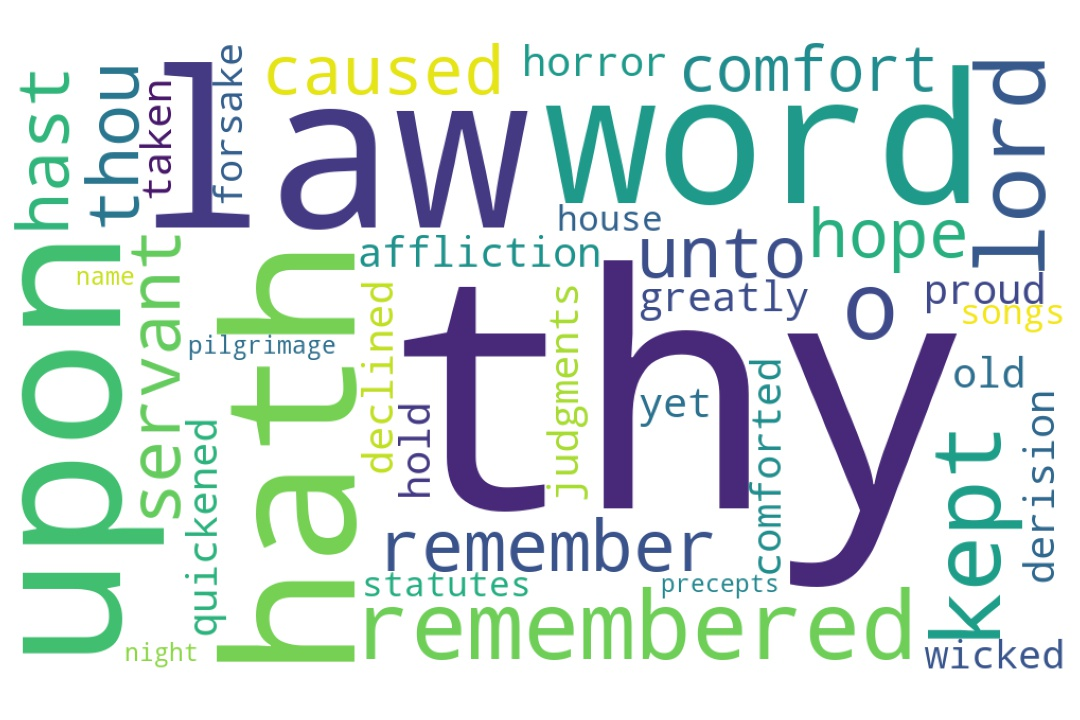
\includegraphics[width=\linewidth]{19OT-Psalms/Psalm119-49-56-WordCloud.jpg}
  \caption{Psalm 119:49-56 Word Cloud}
  \label{fig:Psalm 119:49-56 word Cloud}
\end{figure}

\marginpar{\scriptsize \centering \fcolorbox{bone}{lime}{\textbf{SONGS IN THE NIGHT}}\\ (Psalm 119:49-56) \begin{compactenum}[I.][8]
\item A \textbf{Servant} responding to God \index[scripture]{Psalms!Psa 119:049} (Psa 119:49)
\item The \textbf{Source} of them \index[scripture]{Psalms!Psa 119:049} (Psa 119:49)
\item The \textbf{Solace} they provide \index[scripture]{Psalms!Psa 119:050} (Psa 119:50)
\item The \textbf{Security} that results \index[scripture]{Psalms!Psa 119:051}  (Psa 119:51)
\item The \textbf{Sentencing} they bring to mind \index[scripture]{Psalms!Psa 119:052}(Psa 119:52)
\begin{compactenum}[A.]
\item Ridicule from the ungodly
\item A promised response to this from God
\item Eventual judgment of evil
\end{compactenum}
\item A \textbf{Sunshine} afterwards \index[scripture]{Psalms!Psalm 119:054}\index[scripture]{Psalms!Psa 119:054} (Psa 119:54, 55)
\item The \textbf{Substance} of it all (God's precepts) \index[scripture]{Psalms!Psa 119:056} (Psa 119:56)
\end{compactenum}}

\section*{Zain}
\footnote{\textcolor[cmyk]{0.99998,1,0,0}{\hyperlink{TOC}{Return to end of Table of Contents.}}}\footnote{\href{https://www.audioverse.org/english/audiobibles/books/ENGKJV/O/Ps/1}{\textcolor[cmyk]{0.99998,1,0,0}{Psalm 119 Audio (4:00)}}}\textcolor[cmyk]{0.99998,1,0,0}{Remember the word unto thy \fcolorbox{bone}{lime}{servant}, upon which \fcolorbox{bone}{lime}{thou} hast caused me to hope.}
[50] \textcolor[cmyk]{0.99998,1,0,0}{This \emph{is} my \fcolorbox{bone}{lime}{comfort} in my affliction: for thy word hath quickened me.}
[51] \textcolor[cmyk]{0.99998,1,0,0}{The proud have had me greatly in derision: \emph{yet} have I \fcolorbox{bone}{lime}{not declined} from thy law.}
[52] \textcolor[cmyk]{0.99998,1,0,0}{I remembered thy \fcolorbox{bone}{lime}{judgments} of old, O LORD; and have comforted myself.}
[53] \textcolor[cmyk]{0.99998,1,0,0}{Horror hath taken hold upon me because of the wicked that forsake thy law.}
[54] \textcolor[cmyk]{0.99998,1,0,0}{Thy statutes have been my \fcolorbox{bone}{lime}{songs} in the house of my pilgrimage.}
[55] \textcolor[cmyk]{0.99998,1,0,0}{I have \fcolorbox{bone}{lime}{remembered} thy name, O LORD, in the night, and have kept thy law.}
[56] \textcolor[cmyk]{0.99998,1,0,0}{This I had, because I kept thy \fcolorbox{bone}{lime}{precepts}.}
\index[NWIV]{14!Psalms!Psa 119:049}\index[AWIP]{Remember!Psalms!Psa 119:049}\index[AWIP]{the!Psalms!Psa 119:049}\index[AWIP]{word!Psalms!Psa 119:049}\index[AWIP]{unto!Psalms!Psa 119:049}\index[AWIP]{thy!Psalms!Psa 119:049}\index[AWIP]{servant!Psalms!Psa 119:049}\index[AWIP]{upon!Psalms!Psa 119:049}\index[AWIP]{which!Psalms!Psa 119:049}\index[AWIP]{thou!Psalms!Psa 119:049}\index[AWIP]{hast!Psalms!Psa 119:049}\index[AWIP]{caused!Psalms!Psa 119:049}\index[AWIP]{me!Psalms!Psa 119:049}\index[AWIP]{to!Psalms!Psa 119:049}\index[AWIP]{hope!Psalms!Psa 119:049}

\index[NWIV]{13!Psalms!Psa 119:050}\index[AWIP]{This!Psalms!Psa 119:050}\index[AWIP]{\emph{is}!Psalms!Psa 119:050}\index[AWIP]{my!Psalms!Psa 119:050}\index[AWIP]{comfort!Psalms!Psa 119:050}\index[AWIP]{in!Psalms!Psa 119:050}\index[AWIP]{my!Psalms!Psa 119:050 (2)}\index[AWIP]{affliction!Psalms!Psa 119:050}\index[AWIP]{for!Psalms!Psa 119:050}\index[AWIP]{thy!Psalms!Psa 119:050}\index[AWIP]{word!Psalms!Psa 119:050}\index[AWIP]{hath!Psalms!Psa 119:050}\index[AWIP]{quickened!Psalms!Psa 119:050}\index[AWIP]{me!Psalms!Psa 119:050}

\index[NWIV]{16!Psalms!Psa 119:051}\index[AWIP]{The!Psalms!Psa 119:051}\index[AWIP]{proud!Psalms!Psa 119:051}\index[AWIP]{have!Psalms!Psa 119:051}\index[AWIP]{had!Psalms!Psa 119:051}\index[AWIP]{me!Psalms!Psa 119:051}\index[AWIP]{greatly!Psalms!Psa 119:051}\index[AWIP]{in!Psalms!Psa 119:051}\index[AWIP]{derision!Psalms!Psa 119:051}\index[AWIP]{\emph{yet}!Psalms!Psa 119:051}\index[AWIP]{have!Psalms!Psa 119:051 (2)}\index[AWIP]{I!Psalms!Psa 119:051}\index[AWIP]{not!Psalms!Psa 119:051}\index[AWIP]{declined!Psalms!Psa 119:051}\index[AWIP]{from!Psalms!Psa 119:051}\index[AWIP]{thy!Psalms!Psa 119:051}\index[AWIP]{law!Psalms!Psa 119:051}\index[PNIP]{I!Psalms!Psa 119:051}

\index[NWIV]{12!Psalms!Psa 119:052}\index[AWIP]{I!Psalms!Psa 119:052}\index[AWIP]{remembered!Psalms!Psa 119:052}\index[AWIP]{thy!Psalms!Psa 119:052}\index[AWIP]{judgments!Psalms!Psa 119:052}\index[AWIP]{of!Psalms!Psa 119:052}\index[AWIP]{old!Psalms!Psa 119:052}\index[AWIP]{O!Psalms!Psa 119:052}\index[AWIP]{LORD!Psalms!Psa 119:052}\index[AWIP]{and!Psalms!Psa 119:052}\index[AWIP]{have!Psalms!Psa 119:052}\index[AWIP]{comforted!Psalms!Psa 119:052}\index[AWIP]{myself!Psalms!Psa 119:052}\index[PNIP]{I!Psalms!Psa 119:052}\index[PNIP]{LORD!Psalms!Psa 119:052}

\index[NWIV]{14!Psalms!Psa 119:053}\index[AWIP]{Horror!Psalms!Psa 119:053}\index[AWIP]{hath!Psalms!Psa 119:053}\index[AWIP]{taken!Psalms!Psa 119:053}\index[AWIP]{hold!Psalms!Psa 119:053}\index[AWIP]{upon!Psalms!Psa 119:053}\index[AWIP]{me!Psalms!Psa 119:053}\index[AWIP]{because!Psalms!Psa 119:053}\index[AWIP]{of!Psalms!Psa 119:053}\index[AWIP]{the!Psalms!Psa 119:053}\index[AWIP]{wicked!Psalms!Psa 119:053}\index[AWIP]{that!Psalms!Psa 119:053}\index[AWIP]{forsake!Psalms!Psa 119:053}\index[AWIP]{thy!Psalms!Psa 119:053}\index[AWIP]{law!Psalms!Psa 119:053}

\index[NWIV]{12!Psalms!Psa 119:054}\index[AWIP]{Thy!Psalms!Psa 119:054}\index[AWIP]{statutes!Psalms!Psa 119:054}\index[AWIP]{have!Psalms!Psa 119:054}\index[AWIP]{been!Psalms!Psa 119:054}\index[AWIP]{my!Psalms!Psa 119:054}\index[AWIP]{songs!Psalms!Psa 119:054}\index[AWIP]{in!Psalms!Psa 119:054}\index[AWIP]{the!Psalms!Psa 119:054}\index[AWIP]{house!Psalms!Psa 119:054}\index[AWIP]{of!Psalms!Psa 119:054}\index[AWIP]{my!Psalms!Psa 119:054 (2)}\index[AWIP]{pilgrimage!Psalms!Psa 119:054}

\index[NWIV]{15!Psalms!Psa 119:055}\index[AWIP]{I!Psalms!Psa 119:055}\index[AWIP]{have!Psalms!Psa 119:055}\index[AWIP]{remembered!Psalms!Psa 119:055}\index[AWIP]{thy!Psalms!Psa 119:055}\index[AWIP]{name!Psalms!Psa 119:055}\index[AWIP]{O!Psalms!Psa 119:055}\index[AWIP]{LORD!Psalms!Psa 119:055}\index[AWIP]{in!Psalms!Psa 119:055}\index[AWIP]{the!Psalms!Psa 119:055}\index[AWIP]{night!Psalms!Psa 119:055}\index[AWIP]{and!Psalms!Psa 119:055}\index[AWIP]{have!Psalms!Psa 119:055 (2)}\index[AWIP]{kept!Psalms!Psa 119:055}\index[AWIP]{thy!Psalms!Psa 119:055 (2)}\index[AWIP]{law!Psalms!Psa 119:055}\index[PNIP]{I!Psalms!Psa 119:055}\index[PNIP]{LORD!Psalms!Psa 119:055}

\index[NWIV]{8!Psalms!Psa 119:056}\index[AWIP]{This!Psalms!Psa 119:056}\index[AWIP]{I!Psalms!Psa 119:056}\index[AWIP]{had!Psalms!Psa 119:056}\index[AWIP]{because!Psalms!Psa 119:056}\index[AWIP]{I!Psalms!Psa 119:056 (2)}\index[AWIP]{kept!Psalms!Psa 119:056}\index[AWIP]{thy!Psalms!Psa 119:056}\index[AWIP]{precepts!Psalms!Psa 119:056}\index[PNIP]{I!Psalms!Psa 119:056}


\section{Psalm 119:49-56 Outlines}

\subsection{My Outlines}

\subsubsection{Songs in the Night}
\index[speaker]{Keith Anthony!Psalm 119:048-056 (Songs in the Night)}
\index[series]{Psalms (Keith Anthony)!Psalm 119:048-056 (Songs in the Night)}
\index[date]{2016/05/01!Psalm 119:048-056 (Songs in the Night) (Keith Anthony)}
\textbf{Lineage}: adapted from S. Conway.\\
\textbf{Introduction}: The comfort of God in time of trial.
\begin{compactenum}[I.]
\item A \textbf{Servant} responding to God \index[scripture]{Psalms!Psa 119:049} (Psa 119:49)
\item The \textbf{Source} of them \index[scripture]{Psalms!Psa 119:049} (Psa 119:49)
\item The \textbf{Solace} they provide \index[scripture]{Psalms!Psa 119:050} (Psa 119:50)
\item The \textbf{Security} that results \index[scripture]{Psalms!Psa 119:051}  (Psa 119:51)
\item The \textbf{Sentencing} they bring to mind \index[scripture]{Psalms!Psa 119:052}(Psa 119:52)
\begin{compactenum}[A.]
\item Ridicule from the ungodly
\item A promised response to this from God
\item Eventual judgment of evil
\end{compactenum}
\item A \textbf{Sunshine} afterwards \index[scripture]{Psalms!Psalm 119:054}\index[scripture]{Psalms!Psa 119:054} (Psa 119:54, 55)
\item The \textbf{Substance} of it all (God's precepts) \index[scripture]{Psalms!Psa 119:056} (Psa 119:56)
\end{compactenum}


%\subsection{Outlines from Others}


\section{Psalm 119:49-56 Comments}




\subsection{Psalm119:49-56 Repeated Phrases}


%%%%%%%%%%
%%%%%%%%%%
\normalsize
 
\begin{center}
\begin{longtable}{|c|c|}
\caption[Psalm119:49-56 Repeated Phrases]{Psalm119:49-56 Repeated Phrases}\label{table:Repeated Phrases Psalm119:49-56} \\
\hline \multicolumn{1}{|c|}{\textbf{Phrase}} & \multicolumn{1}{c|}{\textbf{Frequency}} \\ \hline 
\endfirsthead
 
\multicolumn{2}{c}
{{\bfseries \tablename\ \thetable{} -- continued from previous page}} \\  
\hline \multicolumn{1}{|c|}{\textbf{Phrase}} & \multicolumn{1}{c|}{\textbf{Frequency}} \\ \hline 
\endhead
 
\hline \multicolumn{2}{c}{{ }} \\ \hline
\endfoot 
thy law & 3\\ \hline 
\end{longtable}
\end{center}



%%%%%%%%%%
%%%%%%%%%%



\section{Psalm  119:49-56 Word Statistics}


%%%%%%%%%%
%%%%%%%%%%
\normalsize
 
\begin{center}
\begin{longtable}{l|c|c|c|c}
\caption[Psalm  119:49-56 Statistics]{Psalm  119:49-56 Statistics}\label{table:Statistics for Psalm  119:49-56} \\
\hline \multicolumn{1}{|c|}{\textbf{Verse(s)}} & \multicolumn{1}{|c|}{\textbf{Count}} & \multicolumn{1}{|c|}{\textbf{Unique}} & \multicolumn{1}{|c|}{\textbf{Italics}} & \multicolumn{1}{|c|}{\textbf{Uniq Italic}}  \\ \hline 
\endfirsthead
 
\multicolumn{5}{c}
{{\bfseries \tablename\ \thetable{} -- continued from previous page}} \\  
\hline \multicolumn{1}{|c|}{\textbf{Verse(s)}} & \multicolumn{1}{|c|}{\textbf{Count}} & \multicolumn{1}{|c|}{\textbf{Unique}} & \multicolumn{1}{|c|}{\textbf{Italics}} & \multicolumn{1}{|c|}{\textbf{Uniq Italic}}  \\ \hline 
\endhead
 
\hline \multicolumn{5}{|r|}{{Continued if needed}} \\ \hline
\endfoot 
49 & 14 & 14 & 0 & 0\\ \hline
50 & 13 & 12 & 1 & 1\\ \hline
51 & 16 & 15 & 1 & 1\\ \hline
52 & 12 & 12 & 0 & 0\\ \hline
53 & 14 & 14 & 0 & 0\\ \hline
54 & 12 & 11 & 0 & 0\\ \hline
55 & 15 & 13 & 0 & 0\\ \hline
56 & 8 & 7 & 0 & 0\\ \hline
Total & 104 & 61 & 2 & 2
\end{longtable}
\end{center}



%%%%%%%%%%
%%%%%%%%%%


\subsection{Psalm  119:49-56 Words by Frequency}


%%%%%%%%%%
%%%%%%%%%%
\normalsize
 
\begin{center}
\begin{longtable}{l|r}
\caption[Psalm  119:49-56 Words by Frequency]{Psalm  119:49-56 Words by Frequency}\label{table:WordsbyFrequency for Psalm  119:49-56} \\
\hline \multicolumn{1}{|c|}{\textbf{Word}} & \multicolumn{1}{c|}{\textbf{Frequency}} \\ \hline 
\endfirsthead
 
\multicolumn{2}{c}
{{\bfseries \tablename\ \thetable{} -- continued from previous page}} \\  
\hline \multicolumn{1}{|c|}{\textbf{Word}} & \multicolumn{1}{c|}{\textbf{Frequency}} \\ \hline 
\endhead
 
\hline \multicolumn{2}{c}{{ }} \\ \hline
\endfoot 
thy & 8\\ \hline 
have & 6\\ \hline 
I & 5\\ \hline 
the & 4\\ \hline 
me & 4\\ \hline 
my & 4\\ \hline 
in & 4\\ \hline 
law & 3\\ \hline 
of & 3\\ \hline 
word & 2\\ \hline 
upon & 2\\ \hline 
This & 2\\ \hline 
hath & 2\\ \hline 
had & 2\\ \hline 
remembered & 2\\ \hline 
O & 2\\ \hline 
LORD & 2\\ \hline 
and & 2\\ \hline 
because & 2\\ \hline 
kept & 2\\ \hline 
Remember & 1\\ \hline 
unto & 1\\ \hline 
servant & 1\\ \hline 
which & 1\\ \hline 
thou & 1\\ \hline 
hast & 1\\ \hline 
caused & 1\\ \hline 
to & 1\\ \hline 
hope & 1\\ \hline 
\emph{is} & 1\\ \hline 
comfort & 1\\ \hline 
affliction & 1\\ \hline 
for & 1\\ \hline 
quickened & 1\\ \hline 
The & 1\\ \hline 
proud & 1\\ \hline 
greatly & 1\\ \hline 
derision & 1\\ \hline 
\emph{yet} & 1\\ \hline 
not & 1\\ \hline 
declined & 1\\ \hline 
from & 1\\ \hline 
judgments & 1\\ \hline 
old & 1\\ \hline 
comforted & 1\\ \hline 
myself & 1\\ \hline 
Horror & 1\\ \hline 
taken & 1\\ \hline 
hold & 1\\ \hline 
wicked & 1\\ \hline 
that & 1\\ \hline 
forsake & 1\\ \hline 
Thy & 1\\ \hline 
statutes & 1\\ \hline 
been & 1\\ \hline 
songs & 1\\ \hline 
house & 1\\ \hline 
pilgrimage & 1\\ \hline 
name & 1\\ \hline 
night & 1\\ \hline 
precepts & 1\\ \hline 
\end{longtable}
\end{center}



%%%%%%%%%%
%%%%%%%%%%


\subsection{Psalm  119:49-56 Words Alphabetically}


%%%%%%%%%%
%%%%%%%%%%
\normalsize
 
\begin{center}
\begin{longtable}{l|r}
\caption[Psalm  119:49-56 Words Alphabetically]{Psalm  119:49-56 Words Alphabetically}\label{table:WordsAlphabetically for Psalm  119:49-56} \\
\hline \multicolumn{1}{|c|}{\textbf{Word}} & \multicolumn{1}{c|}{\textbf{Frequency}} \\ \hline 
\endfirsthead
 
\multicolumn{2}{c}
{{\bfseries \tablename\ \thetable{} -- continued from previous page}} \\  
\hline \multicolumn{1}{|c|}{\textbf{Word}} & \multicolumn{1}{c|}{\textbf{Frequency}} \\ \hline 
\endhead
 
\hline \multicolumn{2}{c}{{ }} \\ \hline
\endfoot 
Horror & 1\\ \hline 
I & 5\\ \hline 
LORD & 2\\ \hline 
O & 2\\ \hline 
Remember & 1\\ \hline 
The & 1\\ \hline 
This & 2\\ \hline 
Thy & 1\\ \hline 
\emph{is} & 1\\ \hline 
\emph{yet} & 1\\ \hline 
affliction & 1\\ \hline 
and & 2\\ \hline 
because & 2\\ \hline 
been & 1\\ \hline 
caused & 1\\ \hline 
comfort & 1\\ \hline 
comforted & 1\\ \hline 
declined & 1\\ \hline 
derision & 1\\ \hline 
for & 1\\ \hline 
forsake & 1\\ \hline 
from & 1\\ \hline 
greatly & 1\\ \hline 
had & 2\\ \hline 
hast & 1\\ \hline 
hath & 2\\ \hline 
have & 6\\ \hline 
hold & 1\\ \hline 
hope & 1\\ \hline 
house & 1\\ \hline 
in & 4\\ \hline 
judgments & 1\\ \hline 
kept & 2\\ \hline 
law & 3\\ \hline 
me & 4\\ \hline 
my & 4\\ \hline 
myself & 1\\ \hline 
name & 1\\ \hline 
night & 1\\ \hline 
not & 1\\ \hline 
of & 3\\ \hline 
old & 1\\ \hline 
pilgrimage & 1\\ \hline 
precepts & 1\\ \hline 
proud & 1\\ \hline 
quickened & 1\\ \hline 
remembered & 2\\ \hline 
servant & 1\\ \hline 
songs & 1\\ \hline 
statutes & 1\\ \hline 
taken & 1\\ \hline 
that & 1\\ \hline 
the & 4\\ \hline 
thou & 1\\ \hline 
thy & 8\\ \hline 
to & 1\\ \hline 
unto & 1\\ \hline 
upon & 2\\ \hline 
which & 1\\ \hline 
wicked & 1\\ \hline 
word & 2\\ \hline 
\end{longtable}
\end{center}



%%%%%%%%%%
%%%%%%%%%%


\subsection{Psalm  119:49-56 Words by Length}


%%%%%%%%%%
%%%%%%%%%%
\normalsize
 
\begin{center}
\begin{longtable}{l|p{3.75in}}
\caption[Psalm  119:49-56 Words by Length]{Psalm  119:49-56 Words by Length}\label{table:WordsAlphabetically for Psalm  119:49-56} \\
\hline \multicolumn{1}{|c|}{\textbf{Length}} & \multicolumn{1}{c|}{\textbf{Words}} \\ \hline 
\endfirsthead
\hline \multicolumn{1}{|c|}{\textbf{Length}} & \multicolumn{1}{c|}{\textbf{Words}} \\ \hline 
\multicolumn{2}{c}
{{\bfseries \tablename\ \thetable{} -- continued from previous page}} \\  
\hline \multicolumn{1}{|c|}{\textbf{Word}} & \multicolumn{1}{c|}{\textbf{Frequency}} \\ \hline 
\endhead
 
\hline \multicolumn{2}{c}{{ }} \\ \hline
\endfoot 
1 & I, O\\ \hline 
2 & me, to, \emph{is}, my, in, of\\ \hline 
3 & the, thy, for, The, had, \emph{yet}, not, law, old, and, Thy\\ \hline 
4 & word, unto, upon, thou, hast, hope, This, hath, have, from, LORD, hold, that, been, name, kept\\ \hline 
5 & which, proud, taken, songs, house, night\\ \hline 
6 & caused, myself, Horror, wicked\\ \hline 
7 & servant, comfort, greatly, because, forsake\\ \hline 
8 & Remember, derision, declined, statutes, precepts\\ \hline 
9 & quickened, judgments, comforted\\ \hline 
10 & affliction, remembered, pilgrimage\\ \hline 
\end{longtable}
\end{center}



%%%%%%%%%%
%%%%%%%%%%



\input{19OT-Psalms/Psalm119-49-56-Devotionals}

 \chapter{Proverb 16}
 
\begin{figure}
  \includegraphics[width=\linewidth]{20OT-Proverbs/Proverb16-Wordcloud.jpg}
  \caption{Proverb 16 Word Cloud}
  \label{fig:Proverb 16 word Cloud}
\end{figure}

\marginpar{\scriptsize \centering \fcolorbox{bone}{lime}{\textbf{PRAYERS FOR THE FAITHFUL}}\\ (Proverb 16:1-33) \begin{compactenum}[I.][8]
    \item \textbf{Prepare my Heart}  \index[scripture]{Proverbs!Pro 16:01}(Pro 16:1)
    \item \textbf{Peruse my Ways} \index[scripture]{Proverbs!Pro 16:02}(Pro 16:2)
    \item \textbf{Purify my Thoughts} \index[scripture]{Proverbs!Pro 16:03}(Pro 16:3)
    \item \textbf{Point out the Path} \index[scripture]{Proverbs!Pro 16:09}(Pro 16:9)
    \item \textbf{Passify my Anger} \index[scripture]{Proverbs!Pro 16:14}(Pro 16:14)
    \item \textbf{Preserve my Soul} \index[scripture]{Proverbs!Pro 16:17}(Pro 16:17)
    \item \textbf{Impart Wisdom} \index[scripture]{Proverbs!Pro 16:21}(Pro 16:21)
\end{compactenum}}

\marginpar{\scriptsize \centering \fcolorbox{bone}{yellow}{\textbf{A GODLY MAN}}\\ (Proverb 16:1-33) \begin{compactenum}[I.][8]
    \item Is \textbf{Prepared}  \index[scripture]{Proverbs!Pro 16:01} (Pro 16:1)
    \item Is \textbf{Purposed}  \index[scripture]{Proverbs!Pro 16:03} (Pro 16:3)
    \item Has \textbf{Purged} Iniquity  \index[scripture]{Proverbs!Pro 16:06} (Pro 16:6)
    \item Is \textbf{Peaceable}   \index[scripture]{Proverbs!Pro 16:07} (Pro 16:7)
    \item Is \textbf{Preserved}   \index[scripture]{Proverbs!Pro 16:17} (Pro 16:17)
    \item Is not \textbf{Proud}   \index[scripture]{Proverbs!Pro 16:19} (Pro 16:19)
    \item Is \textbf{Prudent}   \index[scripture]{Proverbs!Pro 16:21} (Pro 16:21)
\end{compactenum}}

\marginpar{\scriptsize \centering \fcolorbox{bone}{black}{\textbf{\textcolor[cmyk]{0,0,0,0}{GOD IN CONTROL}}}\\ (Proverb 16) 
 \begin{compactenum}[I.][8]
	\item \textbf{Determined Spirits} \index[scripture]{Proverbs!Pro 16:09} (Pro 16:9)
	\item \textbf{Directed Steps}  \index[scripture]{Proverbs!Pro 16:09} (Pro 16:9)
	\item A \textbf{Divine Sentence}  \index[scripture]{Proverbs!Pro 16:10}  (Pro 16:10)
	\item \textbf{Destroyed Soul}  \index[scripture]{Proverbs!Pro 16:18}  (Pro 16:18)
	\item A \textbf{Delighted Soul}  \index[scripture]{Proverbs!Pro 16:19}  (Pro 16:19)
	\item \textbf{Dug-up Sorrows}  \index[scripture]{Proverbs!Pro 16:27} (Pro 16:27)
	\item A \textbf{Disciplined Spirit}  \index[scripture]{Proverbs!Pro 16:32} (Pro 16:32)
\end{compactenum}}


\marginpar{\scriptsize \centering \fcolorbox{bone}{blue}{\textbf{\textcolor[cmyk]{0,0,0,0}{DETAILS}}}\\ (Proverb 16) 
 \begin{compactenum}[I.][8]

 	\item The \textbf{Works} \index[scripture]{Proverbs!Pro 16:03}(Pro 16:3)
	\item The \textbf{Wicked} \index[scripture]{Proverbs!Pro 16:04}(Pro 16:4)
	\item The \textbf{Ways} \index[scripture]{Proverbs!Pro 16:07}(Pro 16:7)
	\item The \textbf{Way} \index[scripture]{Proverbs!Pro 16:09}\index[scripture]{Proverbs!Pro 16:17}\index[scripture]{Proverbs!Pro 16:25}\index[scripture]{Proverbs!Pro 16:29}\index[scripture]{Proverbs!Pro 16:31}(Pro 16:9, 17, 25, 29, 31)
	\item The \textbf{Weights} \index[scripture]{Proverbs!Pro 16:11}(Pro 16:11)
	\item The \textbf{Wisdom} \index[scripture]{Proverbs!Pro 16:16}(Pro 16:16)
	\item The \textbf{Wellspring} \index[scripture]{Proverbs!Pro 16:22}(Pro 16:22)
	\item The \textbf{Words} \index[scripture]{Proverbs!Pro 16:24}(Pro 16:24)
	\item The \textbf{Whisperer} \index[scripture]{Proverbs!Pro 16:28}(Pro 16:28)
\end{compactenum}}








\footnote{\textcolor[cmyk]{0.99998,1,0,0}{\hyperlink{TOC}{Return to end of Table of Contents.}}}\footnote{\href{https://audiobible.com/bible/proverbs_16.html}{\textcolor[cmyk]{0.99998,1,0,0}{Proverbs Audio}}}\textcolor[cmyk]{0.99998,1,0,0}{The \fcolorbox{bone}{lime}{preparations of the heart} in man, and the answer of the tongue, \emph{is} from the LORD.}
[2] \textcolor[cmyk]{0.99998,1,0,0}{All the ways of a man \emph{are} clean in his own eyes; but the \fcolorbox{bone}{lime}{LORD} \fcolorbox{bone}{lime}{weigheth} \fcolorbox{bone}{lime}{the} \fcolorbox{bone}{lime}{spirits}.}
[3] \textcolor[cmyk]{0.99998,1,0,0}{Commit thy works unto the LORD, and thy \fcolorbox{bone}{lime}{thoughts shall be} \fcolorbox{bone}{lime}{established}.}
[4] \textcolor[cmyk]{0.99998,1,0,0}{The LORD hath made all \emph{things} for himself: yea, even the wicked for the day of evil.}
[5] \textcolor[cmyk]{0.99998,1,0,0}{Every one \emph{that} \emph{is} proud in heart \emph{is} an abomination to the LORD: \emph{though} hand \emph{join} in hand, he shall not be unpunished.}
[6] \textcolor[cmyk]{0.99998,1,0,0}{By mercy and truth iniquity is purged: and by the fear of the LORD \emph{men} depart from evil.}
[7] \textcolor[cmyk]{0.99998,1,0,0}{When a man's ways please the LORD, he maketh even his enemies to be at peace with him.}
[8] \textcolor[cmyk]{0.99998,1,0,0}{Better \emph{is} a little with \fcolorbox{bone}{MYGOLD}{righteousness} than great revenues without right.}
[9] \textcolor[cmyk]{0.99998,1,0,0}{A man's heart deviseth his way: but the \fcolorbox{bone}{lime}{LORD directeth his steps}.}
[10] \textcolor[cmyk]{0.99998,1,0,0}{A divine sentence \emph{is} in the lips of the king: his mouth \fcolorbox{bone}{MYGOLD}{transgresseth} not in judgment.}
[11] \textcolor[cmyk]{0.99998,1,0,0}{A just weight and balance \emph{are} the LORD'S: all the weights of the bag \emph{are} his work.}
[12] \textcolor[cmyk]{0.99998,1,0,0}{\emph{It} \emph{is} an abomination to kings to commit wickedness: for the throne is established by \fcolorbox{bone}{MYGOLD}{righteousness}.}
[13] \textcolor[cmyk]{0.99998,1,0,0}{Righteous lips \emph{are} the delight of kings; and they love him that speaketh right.}
[14] \textcolor[cmyk]{0.99998,1,0,0}{The wrath of a king \emph{is} \emph{as} messengers of death: but a \fcolorbox{bone}{lime}{wise man will pacify it}.}
[15] \textcolor[cmyk]{0.99998,1,0,0}{In the light of the king's countenance \emph{is} life; and his favour \emph{is} as a cloud of the latter rain.}
[16] \textcolor[cmyk]{0.99998,1,0,0}{How much better \emph{is} \emph{it} to get wisdom than gold! and to get \fcolorbox{bone}{MYGOLD}{understanding} rather to be chosen than silver!}
[17] \textcolor[cmyk]{0.99998,1,0,0}{The highway of the upright \emph{is} to depart from evil: he that keepeth his way \fcolorbox{bone}{lime}{preserveth} his soul.}
[18] \textcolor[cmyk]{0.99998,1,0,0}{Pride \emph{goeth} before destruction, and an haughty spirit before a fall.}
[19] \textcolor[cmyk]{0.99998,1,0,0}{Better \emph{it} \emph{is} \emph{to} \emph{be} of an humble spirit with the lowly, than to divide the spoil with the proud.}
[20] \textcolor[cmyk]{0.99998,1,0,0}{He that handleth a matter wisely shall find good: and whoso trusteth in the LORD, happy \emph{is} he.}
[21] \textcolor[cmyk]{0.99998,1,0,0}{The \fcolorbox{bone}{lime}{wise in heart} shall be called prudent: and the sweetness of the lips increaseth learning.}
[22] \textcolor[cmyk]{0.99998,1,0,0}{\fcolorbox{bone}{MYGOLD}{Understanding} \emph{is} a wellspring of life unto him that hath it: but the instruction of fools \emph{is} folly.}\footnote{\textbf{Proverbs 18:4} - The words of a man’s mouth are as deep waters, and the wellspring of wisdom as a flowing brook.}\marginpar{ \scriptsize  {\textcolor[rgb]{0.00,0.545,0.269}{$\rightarrow$``wellspring'' found ONLY here and in Proverbs 18:4.}}}
[23] \textcolor[cmyk]{0.99998,1,0,0}{The heart of the wise teacheth his mouth, and addeth learning to his lips.}
[24] \textcolor[cmyk]{0.99998,1,0,0}{Pleasant words \emph{are} \emph{as} an honeycomb, sweet to the soul, and health to the bones.}
[25] \textcolor[cmyk]{0.99998,1,0,0}{There is a way that seemeth right unto a man, but the end thereof \emph{are} the ways of death.}
[26] \textcolor[cmyk]{0.99998,1,0,0}{He that laboureth laboureth for himself; for his mouth craveth it of him.}
[27] \textcolor[cmyk]{0.99998,1,0,0}{An ungodly man diggeth up evil: and in his lips \emph{there} \emph{is} as a burning fire.}
[28] \textcolor[cmyk]{0.99998,1,0,0}{A froward man soweth strife: and a whisperer separateth chief friends.}\footnote{\textbf{Proverb 6:14} - Frowardness is in his heart, he deviseth mischief continually; he soweth discord.}\footnote{\textbf{Proverb 6:19} - A false witness that speaketh lies, and he that soweth discord among brethren.}
[29] \textcolor[cmyk]{0.99998,1,0,0}{A violent man enticeth his neighbour, and leadeth him into the way \emph{that} \emph{is} not good.}
[30] \textcolor[cmyk]{0.99998,1,0,0}{He shutteth his eyes to devise froward things: moving his lips he bringeth evil to pass.}
[31] \textcolor[cmyk]{0.99998,1,0,0}{The hoary head \emph{is} a crown of glory, \emph{if} it be found in the way of \fcolorbox{bone}{MYGOLD}{righteousness}.}
[32] \textcolor[cmyk]{0.99998,1,0,0}{\emph{He} \emph{that} \emph{is} slow to anger \emph{is} better than the mighty; and he that ruleth his spirit than he that taketh a city.}
[33] \textcolor[cmyk]{0.99998,1,0,0}{The lot is cast into the lap; but the whole disposing thereof \emph{is} of the LORD.}



\index[NWIV]{17!Proverbs!Pro 16:1}\index[AWIP]{The!Proverbs!Pro 16:1}\index[AWIP]{preparations!Proverbs!Pro 16:1}\index[AWIP]{of!Proverbs!Pro 16:1}\index[AWIP]{of!Proverbs!Pro 16:1 (2)}\index[AWIP]{the!Proverbs!Pro 16:1}\index[AWIP]{the!Proverbs!Pro 16:1 (2)}\index[AWIP]{the!Proverbs!Pro 16:1 (3)}\index[AWIP]{the!Proverbs!Pro 16:1 (4)}\index[AWIP]{heart!Proverbs!Pro 16:1}\index[AWIP]{in!Proverbs!Pro 16:1}\index[AWIP]{man!Proverbs!Pro 16:1}\index[AWIP]{and!Proverbs!Pro 16:1}\index[AWIP]{answer!Proverbs!Pro 16:1}\index[AWIP]{tongue!Proverbs!Pro 16:1}\index[AWIP]{\emph{is}!Proverbs!Pro 16:1}\index[AWIP]{from!Proverbs!Pro 16:1}\index[AWIP]{LORD!Proverbs!Pro 16:1}\index[AWIP]{\emph{is}!Proverbs!Pro 16:1}

\index[NWIV]{18!Proverbs!Pro 16:2}\index[AWIP]{All!Proverbs!Pro 16:2}\index[AWIP]{the!Proverbs!Pro 16:2}\index[AWIP]{the!Proverbs!Pro 16:2 (2)}\index[AWIP]{the!Proverbs!Pro 16:2 (3)}\index[AWIP]{ways!Proverbs!Pro 16:2}\index[AWIP]{of!Proverbs!Pro 16:2}\index[AWIP]{a!Proverbs!Pro 16:2}\index[AWIP]{man!Proverbs!Pro 16:2}\index[AWIP]{\emph{are}!Proverbs!Pro 16:2}\index[AWIP]{clean!Proverbs!Pro 16:2}\index[AWIP]{in!Proverbs!Pro 16:2}\index[AWIP]{his!Proverbs!Pro 16:2}\index[AWIP]{own!Proverbs!Pro 16:2}\index[AWIP]{eyes!Proverbs!Pro 16:2}\index[AWIP]{but!Proverbs!Pro 16:2}\index[AWIP]{LORD!Proverbs!Pro 16:2}\index[AWIP]{weigheth!Proverbs!Pro 16:2}\index[AWIP]{spirits!Proverbs!Pro 16:2}\index[AWIP]{\emph{are}!Proverbs!Pro 16:2}

\index[NWIV]{12!Proverbs!Pro 16:3}\index[AWIP]{Commit!Proverbs!Pro 16:3}\index[AWIP]{thy!Proverbs!Pro 16:3}\index[AWIP]{thy!Proverbs!Pro 16:3 (2)}\index[AWIP]{works!Proverbs!Pro 16:3}\index[AWIP]{unto!Proverbs!Pro 16:3}\index[AWIP]{the!Proverbs!Pro 16:3}\index[AWIP]{LORD!Proverbs!Pro 16:3}\index[AWIP]{and!Proverbs!Pro 16:3}\index[AWIP]{thoughts!Proverbs!Pro 16:3}\index[AWIP]{shall!Proverbs!Pro 16:3}\index[AWIP]{be!Proverbs!Pro 16:3}\index[AWIP]{established!Proverbs!Pro 16:3}

\index[NWIV]{17!Proverbs!Pro 16:4}\index[AWIP]{The!Proverbs!Pro 16:4}\index[AWIP]{LORD!Proverbs!Pro 16:4}\index[AWIP]{hath!Proverbs!Pro 16:4}\index[AWIP]{made!Proverbs!Pro 16:4}\index[AWIP]{all!Proverbs!Pro 16:4}\index[AWIP]{\emph{things}!Proverbs!Pro 16:4}\index[AWIP]{for!Proverbs!Pro 16:4}\index[AWIP]{for!Proverbs!Pro 16:4 (2)}\index[AWIP]{himself!Proverbs!Pro 16:4}\index[AWIP]{yea!Proverbs!Pro 16:4}\index[AWIP]{even!Proverbs!Pro 16:4}\index[AWIP]{the!Proverbs!Pro 16:4}\index[AWIP]{the!Proverbs!Pro 16:4 (2)}\index[AWIP]{wicked!Proverbs!Pro 16:4}\index[AWIP]{day!Proverbs!Pro 16:4}\index[AWIP]{of!Proverbs!Pro 16:4}\index[AWIP]{evil!Proverbs!Pro 16:4}\index[AWIP]{\emph{things}!Proverbs!Pro 16:4}

\index[NWIV]{23!Proverbs!Pro 16:5}\index[AWIP]{Every!Proverbs!Pro 16:5}\index[AWIP]{one!Proverbs!Pro 16:5}\index[AWIP]{\emph{that}!Proverbs!Pro 16:5}\index[AWIP]{\emph{is}!Proverbs!Pro 16:5}\index[AWIP]{\emph{is}!Proverbs!Pro 16:5 (2)}\index[AWIP]{proud!Proverbs!Pro 16:5}\index[AWIP]{in!Proverbs!Pro 16:5}\index[AWIP]{in!Proverbs!Pro 16:5 (2)}\index[AWIP]{heart!Proverbs!Pro 16:5}\index[AWIP]{an!Proverbs!Pro 16:5}\index[AWIP]{abomination!Proverbs!Pro 16:5}\index[AWIP]{to!Proverbs!Pro 16:5}\index[AWIP]{the!Proverbs!Pro 16:5}\index[AWIP]{LORD!Proverbs!Pro 16:5}\index[AWIP]{\emph{though}!Proverbs!Pro 16:5}\index[AWIP]{hand!Proverbs!Pro 16:5}\index[AWIP]{hand!Proverbs!Pro 16:5 (2)}\index[AWIP]{\emph{join}!Proverbs!Pro 16:5}\index[AWIP]{he!Proverbs!Pro 16:5}\index[AWIP]{shall!Proverbs!Pro 16:5}\index[AWIP]{not!Proverbs!Pro 16:5}\index[AWIP]{be!Proverbs!Pro 16:5}\index[AWIP]{unpunished!Proverbs!Pro 16:5}\index[AWIP]{\emph{that}!Proverbs!Pro 16:5}\index[AWIP]{\emph{is}!Proverbs!Pro 16:5}\index[AWIP]{\emph{is}!Proverbs!Pro 16:5 (2)}\index[AWIP]{\emph{though}!Proverbs!Pro 16:5}\index[AWIP]{\emph{join}!Proverbs!Pro 16:5}

\index[NWIV]{18!Proverbs!Pro 16:6}\index[AWIP]{By!Proverbs!Pro 16:6}\index[AWIP]{mercy!Proverbs!Pro 16:6}\index[AWIP]{and!Proverbs!Pro 16:6}\index[AWIP]{and!Proverbs!Pro 16:6 (2)}\index[AWIP]{truth!Proverbs!Pro 16:6}\index[AWIP]{iniquity!Proverbs!Pro 16:6}\index[AWIP]{is!Proverbs!Pro 16:6}\index[AWIP]{purged!Proverbs!Pro 16:6}\index[AWIP]{by!Proverbs!Pro 16:6}\index[AWIP]{the!Proverbs!Pro 16:6}\index[AWIP]{the!Proverbs!Pro 16:6 (2)}\index[AWIP]{fear!Proverbs!Pro 16:6}\index[AWIP]{of!Proverbs!Pro 16:6}\index[AWIP]{LORD!Proverbs!Pro 16:6}\index[AWIP]{\emph{men}!Proverbs!Pro 16:6}\index[AWIP]{depart!Proverbs!Pro 16:6}\index[AWIP]{from!Proverbs!Pro 16:6}\index[AWIP]{evil!Proverbs!Pro 16:6}\index[AWIP]{\emph{men}!Proverbs!Pro 16:6}

\index[NWIV]{18!Proverbs!Pro 16:7}\index[AWIP]{When!Proverbs!Pro 16:7}\index[AWIP]{a!Proverbs!Pro 16:7}\index[AWIP]{man's!Proverbs!Pro 16:7}\index[AWIP]{ways!Proverbs!Pro 16:7}\index[AWIP]{please!Proverbs!Pro 16:7}\index[AWIP]{the!Proverbs!Pro 16:7}\index[AWIP]{LORD!Proverbs!Pro 16:7}\index[AWIP]{he!Proverbs!Pro 16:7}\index[AWIP]{maketh!Proverbs!Pro 16:7}\index[AWIP]{even!Proverbs!Pro 16:7}\index[AWIP]{his!Proverbs!Pro 16:7}\index[AWIP]{enemies!Proverbs!Pro 16:7}\index[AWIP]{to!Proverbs!Pro 16:7}\index[AWIP]{be!Proverbs!Pro 16:7}\index[AWIP]{at!Proverbs!Pro 16:7}\index[AWIP]{peace!Proverbs!Pro 16:7}\index[AWIP]{with!Proverbs!Pro 16:7}\index[AWIP]{him!Proverbs!Pro 16:7}

\index[NWIV]{11!Proverbs!Pro 16:8}\index[AWIP]{Better!Proverbs!Pro 16:8}\index[AWIP]{\emph{is}!Proverbs!Pro 16:8}\index[AWIP]{a!Proverbs!Pro 16:8}\index[AWIP]{little!Proverbs!Pro 16:8}\index[AWIP]{with!Proverbs!Pro 16:8}\index[AWIP]{righteousness!Proverbs!Pro 16:8}\index[AWIP]{than!Proverbs!Pro 16:8}\index[AWIP]{great!Proverbs!Pro 16:8}\index[AWIP]{revenues!Proverbs!Pro 16:8}\index[AWIP]{without!Proverbs!Pro 16:8}\index[AWIP]{right!Proverbs!Pro 16:8}\index[AWIP]{\emph{is}!Proverbs!Pro 16:8}

\index[NWIV]{12!Proverbs!Pro 16:9}\index[AWIP]{A!Proverbs!Pro 16:9}\index[AWIP]{man's!Proverbs!Pro 16:9}\index[AWIP]{heart!Proverbs!Pro 16:9}\index[AWIP]{deviseth!Proverbs!Pro 16:9}\index[AWIP]{his!Proverbs!Pro 16:9}\index[AWIP]{his!Proverbs!Pro 16:9 (2)}\index[AWIP]{way!Proverbs!Pro 16:9}\index[AWIP]{but!Proverbs!Pro 16:9}\index[AWIP]{the!Proverbs!Pro 16:9}\index[AWIP]{LORD!Proverbs!Pro 16:9}\index[AWIP]{directeth!Proverbs!Pro 16:9}\index[AWIP]{steps!Proverbs!Pro 16:9}

\index[NWIV]{16!Proverbs!Pro 16:10}\index[AWIP]{A!Proverbs!Pro 16:10}\index[AWIP]{divine!Proverbs!Pro 16:10}\index[AWIP]{sentence!Proverbs!Pro 16:10}\index[AWIP]{\emph{is}!Proverbs!Pro 16:10}\index[AWIP]{in!Proverbs!Pro 16:10}\index[AWIP]{in!Proverbs!Pro 16:10 (2)}\index[AWIP]{the!Proverbs!Pro 16:10}\index[AWIP]{the!Proverbs!Pro 16:10 (2)}\index[AWIP]{lips!Proverbs!Pro 16:10}\index[AWIP]{of!Proverbs!Pro 16:10}\index[AWIP]{king!Proverbs!Pro 16:10}\index[AWIP]{his!Proverbs!Pro 16:10}\index[AWIP]{mouth!Proverbs!Pro 16:10}\index[AWIP]{transgresseth!Proverbs!Pro 16:10}\index[AWIP]{not!Proverbs!Pro 16:10}\index[AWIP]{judgment!Proverbs!Pro 16:10}\index[AWIP]{\emph{is}!Proverbs!Pro 16:10}

\index[NWIV]{17!Proverbs!Pro 16:11}\index[AWIP]{A!Proverbs!Pro 16:11}\index[AWIP]{just!Proverbs!Pro 16:11}\index[AWIP]{weight!Proverbs!Pro 16:11}\index[AWIP]{and!Proverbs!Pro 16:11}\index[AWIP]{balance!Proverbs!Pro 16:11}\index[AWIP]{\emph{are}!Proverbs!Pro 16:11}\index[AWIP]{\emph{are}!Proverbs!Pro 16:11 (2)}\index[AWIP]{the!Proverbs!Pro 16:11}\index[AWIP]{the!Proverbs!Pro 16:11 (2)}\index[AWIP]{the!Proverbs!Pro 16:11 (3)}\index[AWIP]{LORD'S!Proverbs!Pro 16:11}\index[AWIP]{all!Proverbs!Pro 16:11}\index[AWIP]{weights!Proverbs!Pro 16:11}\index[AWIP]{of!Proverbs!Pro 16:11}\index[AWIP]{bag!Proverbs!Pro 16:11}\index[AWIP]{his!Proverbs!Pro 16:11}\index[AWIP]{work!Proverbs!Pro 16:11}\index[AWIP]{\emph{are}!Proverbs!Pro 16:11}\index[AWIP]{\emph{are}!Proverbs!Pro 16:11 (2)}

\index[NWIV]{16!Proverbs!Pro 16:12}\index[AWIP]{\emph{It}!Proverbs!Pro 16:12}\index[AWIP]{\emph{is}!Proverbs!Pro 16:12}\index[AWIP]{an!Proverbs!Pro 16:12}\index[AWIP]{abomination!Proverbs!Pro 16:12}\index[AWIP]{to!Proverbs!Pro 16:12}\index[AWIP]{to!Proverbs!Pro 16:12 (2)}\index[AWIP]{kings!Proverbs!Pro 16:12}\index[AWIP]{commit!Proverbs!Pro 16:12}\index[AWIP]{wickedness!Proverbs!Pro 16:12}\index[AWIP]{for!Proverbs!Pro 16:12}\index[AWIP]{the!Proverbs!Pro 16:12}\index[AWIP]{throne!Proverbs!Pro 16:12}\index[AWIP]{is!Proverbs!Pro 16:12}\index[AWIP]{established!Proverbs!Pro 16:12}\index[AWIP]{by!Proverbs!Pro 16:12}\index[AWIP]{righteousness!Proverbs!Pro 16:12}\index[AWIP]{\emph{It}!Proverbs!Pro 16:12}\index[AWIP]{\emph{is}!Proverbs!Pro 16:12}

\index[NWIV]{14!Proverbs!Pro 16:13}\index[AWIP]{Righteous!Proverbs!Pro 16:13}\index[AWIP]{lips!Proverbs!Pro 16:13}\index[AWIP]{\emph{are}!Proverbs!Pro 16:13}\index[AWIP]{the!Proverbs!Pro 16:13}\index[AWIP]{delight!Proverbs!Pro 16:13}\index[AWIP]{of!Proverbs!Pro 16:13}\index[AWIP]{kings!Proverbs!Pro 16:13}\index[AWIP]{and!Proverbs!Pro 16:13}\index[AWIP]{they!Proverbs!Pro 16:13}\index[AWIP]{love!Proverbs!Pro 16:13}\index[AWIP]{him!Proverbs!Pro 16:13}\index[AWIP]{that!Proverbs!Pro 16:13}\index[AWIP]{speaketh!Proverbs!Pro 16:13}\index[AWIP]{right!Proverbs!Pro 16:13}\index[AWIP]{\emph{are}!Proverbs!Pro 16:13}

\index[NWIV]{17!Proverbs!Pro 16:14}\index[AWIP]{The!Proverbs!Pro 16:14}\index[AWIP]{wrath!Proverbs!Pro 16:14}\index[AWIP]{of!Proverbs!Pro 16:14}\index[AWIP]{of!Proverbs!Pro 16:14 (2)}\index[AWIP]{a!Proverbs!Pro 16:14}\index[AWIP]{a!Proverbs!Pro 16:14 (2)}\index[AWIP]{king!Proverbs!Pro 16:14}\index[AWIP]{\emph{is}!Proverbs!Pro 16:14}\index[AWIP]{\emph{as}!Proverbs!Pro 16:14}\index[AWIP]{messengers!Proverbs!Pro 16:14}\index[AWIP]{death!Proverbs!Pro 16:14}\index[AWIP]{but!Proverbs!Pro 16:14}\index[AWIP]{wise!Proverbs!Pro 16:14}\index[AWIP]{man!Proverbs!Pro 16:14}\index[AWIP]{will!Proverbs!Pro 16:14}\index[AWIP]{pacify!Proverbs!Pro 16:14}\index[AWIP]{it!Proverbs!Pro 16:14}\index[AWIP]{\emph{is}!Proverbs!Pro 16:14}\index[AWIP]{\emph{as}!Proverbs!Pro 16:14}

\index[NWIV]{20!Proverbs!Pro 16:15}\index[AWIP]{In!Proverbs!Pro 16:15}\index[AWIP]{the!Proverbs!Pro 16:15}\index[AWIP]{the!Proverbs!Pro 16:15 (2)}\index[AWIP]{the!Proverbs!Pro 16:15 (3)}\index[AWIP]{light!Proverbs!Pro 16:15}\index[AWIP]{of!Proverbs!Pro 16:15}\index[AWIP]{of!Proverbs!Pro 16:15 (2)}\index[AWIP]{king's!Proverbs!Pro 16:15}\index[AWIP]{countenance!Proverbs!Pro 16:15}\index[AWIP]{\emph{is}!Proverbs!Pro 16:15}\index[AWIP]{\emph{is}!Proverbs!Pro 16:15 (2)}\index[AWIP]{life!Proverbs!Pro 16:15}\index[AWIP]{and!Proverbs!Pro 16:15}\index[AWIP]{his!Proverbs!Pro 16:15}\index[AWIP]{favour!Proverbs!Pro 16:15}\index[AWIP]{as!Proverbs!Pro 16:15}\index[AWIP]{a!Proverbs!Pro 16:15}\index[AWIP]{cloud!Proverbs!Pro 16:15}\index[AWIP]{latter!Proverbs!Pro 16:15}\index[AWIP]{rain!Proverbs!Pro 16:15}\index[AWIP]{\emph{is}!Proverbs!Pro 16:15}\index[AWIP]{\emph{is}!Proverbs!Pro 16:15 (2)}

\index[NWIV]{20!Proverbs!Pro 16:16}\index[AWIP]{How!Proverbs!Pro 16:16}\index[AWIP]{much!Proverbs!Pro 16:16}\index[AWIP]{better!Proverbs!Pro 16:16}\index[AWIP]{\emph{is}!Proverbs!Pro 16:16}\index[AWIP]{\emph{it}!Proverbs!Pro 16:16}\index[AWIP]{to!Proverbs!Pro 16:16}\index[AWIP]{to!Proverbs!Pro 16:16 (2)}\index[AWIP]{to!Proverbs!Pro 16:16 (3)}\index[AWIP]{get!Proverbs!Pro 16:16}\index[AWIP]{get!Proverbs!Pro 16:16 (2)}\index[AWIP]{wisdom!Proverbs!Pro 16:16}\index[AWIP]{than!Proverbs!Pro 16:16}\index[AWIP]{than!Proverbs!Pro 16:16 (2)}\index[AWIP]{gold!!Proverbs!Pro 16:16}\index[AWIP]{and!Proverbs!Pro 16:16}\index[AWIP]{understanding!Proverbs!Pro 16:16}\index[AWIP]{rather!Proverbs!Pro 16:16}\index[AWIP]{be!Proverbs!Pro 16:16}\index[AWIP]{chosen!Proverbs!Pro 16:16}\index[AWIP]{silver!!Proverbs!Pro 16:16}\index[AWIP]{\emph{is}!Proverbs!Pro 16:16}\index[AWIP]{\emph{it}!Proverbs!Pro 16:16}

\index[NWIV]{18!Proverbs!Pro 16:17}\index[AWIP]{The!Proverbs!Pro 16:17}\index[AWIP]{highway!Proverbs!Pro 16:17}\index[AWIP]{of!Proverbs!Pro 16:17}\index[AWIP]{the!Proverbs!Pro 16:17}\index[AWIP]{upright!Proverbs!Pro 16:17}\index[AWIP]{\emph{is}!Proverbs!Pro 16:17}\index[AWIP]{to!Proverbs!Pro 16:17}\index[AWIP]{depart!Proverbs!Pro 16:17}\index[AWIP]{from!Proverbs!Pro 16:17}\index[AWIP]{evil!Proverbs!Pro 16:17}\index[AWIP]{he!Proverbs!Pro 16:17}\index[AWIP]{that!Proverbs!Pro 16:17}\index[AWIP]{keepeth!Proverbs!Pro 16:17}\index[AWIP]{his!Proverbs!Pro 16:17}\index[AWIP]{his!Proverbs!Pro 16:17 (2)}\index[AWIP]{way!Proverbs!Pro 16:17}\index[AWIP]{preserveth!Proverbs!Pro 16:17}\index[AWIP]{soul!Proverbs!Pro 16:17}\index[AWIP]{\emph{is}!Proverbs!Pro 16:17}

\index[NWIV]{11!Proverbs!Pro 16:18}\index[AWIP]{Pride!Proverbs!Pro 16:18}\index[AWIP]{\emph{goeth}!Proverbs!Pro 16:18}\index[AWIP]{before!Proverbs!Pro 16:18}\index[AWIP]{before!Proverbs!Pro 16:18 (2)}\index[AWIP]{destruction!Proverbs!Pro 16:18}\index[AWIP]{and!Proverbs!Pro 16:18}\index[AWIP]{an!Proverbs!Pro 16:18}\index[AWIP]{haughty!Proverbs!Pro 16:18}\index[AWIP]{spirit!Proverbs!Pro 16:18}\index[AWIP]{a!Proverbs!Pro 16:18}\index[AWIP]{fall!Proverbs!Pro 16:18}\index[AWIP]{\emph{goeth}!Proverbs!Pro 16:18}

\index[NWIV]{20!Proverbs!Pro 16:19}\index[AWIP]{Better!Proverbs!Pro 16:19}\index[AWIP]{\emph{it}!Proverbs!Pro 16:19}\index[AWIP]{\emph{is}!Proverbs!Pro 16:19}\index[AWIP]{\emph{to}!Proverbs!Pro 16:19}\index[AWIP]{\emph{be}!Proverbs!Pro 16:19}\index[AWIP]{of!Proverbs!Pro 16:19}\index[AWIP]{an!Proverbs!Pro 16:19}\index[AWIP]{humble!Proverbs!Pro 16:19}\index[AWIP]{spirit!Proverbs!Pro 16:19}\index[AWIP]{with!Proverbs!Pro 16:19}\index[AWIP]{with!Proverbs!Pro 16:19 (2)}\index[AWIP]{the!Proverbs!Pro 16:19}\index[AWIP]{the!Proverbs!Pro 16:19 (2)}\index[AWIP]{the!Proverbs!Pro 16:19 (3)}\index[AWIP]{lowly!Proverbs!Pro 16:19}\index[AWIP]{than!Proverbs!Pro 16:19}\index[AWIP]{to!Proverbs!Pro 16:19}\index[AWIP]{divide!Proverbs!Pro 16:19}\index[AWIP]{spoil!Proverbs!Pro 16:19}\index[AWIP]{proud!Proverbs!Pro 16:19}\index[AWIP]{\emph{it}!Proverbs!Pro 16:19}\index[AWIP]{\emph{is}!Proverbs!Pro 16:19}\index[AWIP]{\emph{to}!Proverbs!Pro 16:19}\index[AWIP]{\emph{be}!Proverbs!Pro 16:19}

\index[NWIV]{18!Proverbs!Pro 16:20}\index[AWIP]{He!Proverbs!Pro 16:20}\index[AWIP]{that!Proverbs!Pro 16:20}\index[AWIP]{handleth!Proverbs!Pro 16:20}\index[AWIP]{a!Proverbs!Pro 16:20}\index[AWIP]{matter!Proverbs!Pro 16:20}\index[AWIP]{wisely!Proverbs!Pro 16:20}\index[AWIP]{shall!Proverbs!Pro 16:20}\index[AWIP]{find!Proverbs!Pro 16:20}\index[AWIP]{good!Proverbs!Pro 16:20}\index[AWIP]{and!Proverbs!Pro 16:20}\index[AWIP]{whoso!Proverbs!Pro 16:20}\index[AWIP]{trusteth!Proverbs!Pro 16:20}\index[AWIP]{in!Proverbs!Pro 16:20}\index[AWIP]{the!Proverbs!Pro 16:20}\index[AWIP]{LORD!Proverbs!Pro 16:20}\index[AWIP]{happy!Proverbs!Pro 16:20}\index[AWIP]{\emph{is}!Proverbs!Pro 16:20}\index[AWIP]{he!Proverbs!Pro 16:20}\index[AWIP]{\emph{is}!Proverbs!Pro 16:20}

\index[NWIV]{16!Proverbs!Pro 16:21}\index[AWIP]{The!Proverbs!Pro 16:21}\index[AWIP]{wise!Proverbs!Pro 16:21}\index[AWIP]{in!Proverbs!Pro 16:21}\index[AWIP]{heart!Proverbs!Pro 16:21}\index[AWIP]{shall!Proverbs!Pro 16:21}\index[AWIP]{be!Proverbs!Pro 16:21}\index[AWIP]{called!Proverbs!Pro 16:21}\index[AWIP]{prudent!Proverbs!Pro 16:21}\index[AWIP]{and!Proverbs!Pro 16:21}\index[AWIP]{the!Proverbs!Pro 16:21}\index[AWIP]{the!Proverbs!Pro 16:21 (2)}\index[AWIP]{sweetness!Proverbs!Pro 16:21}\index[AWIP]{of!Proverbs!Pro 16:21}\index[AWIP]{lips!Proverbs!Pro 16:21}\index[AWIP]{increaseth!Proverbs!Pro 16:21}\index[AWIP]{learning!Proverbs!Pro 16:21}

\index[NWIV]{18!Proverbs!Pro 16:22}\index[AWIP]{Understanding!Proverbs!Pro 16:22}\index[AWIP]{\emph{is}!Proverbs!Pro 16:22}\index[AWIP]{\emph{is}!Proverbs!Pro 16:22 (2)}\index[AWIP]{a!Proverbs!Pro 16:22}\index[AWIP]{wellspring!Proverbs!Pro 16:22}\index[AWIP]{of!Proverbs!Pro 16:22}\index[AWIP]{of!Proverbs!Pro 16:22 (2)}\index[AWIP]{life!Proverbs!Pro 16:22}\index[AWIP]{unto!Proverbs!Pro 16:22}\index[AWIP]{him!Proverbs!Pro 16:22}\index[AWIP]{that!Proverbs!Pro 16:22}\index[AWIP]{hath!Proverbs!Pro 16:22}\index[AWIP]{it!Proverbs!Pro 16:22}\index[AWIP]{but!Proverbs!Pro 16:22}\index[AWIP]{the!Proverbs!Pro 16:22}\index[AWIP]{instruction!Proverbs!Pro 16:22}\index[AWIP]{fools!Proverbs!Pro 16:22}\index[AWIP]{folly!Proverbs!Pro 16:22}\index[AWIP]{\emph{is}!Proverbs!Pro 16:22}\index[AWIP]{\emph{is}!Proverbs!Pro 16:22 (2)}

\index[NWIV]{14!Proverbs!Pro 16:23}\index[AWIP]{The!Proverbs!Pro 16:23}\index[AWIP]{heart!Proverbs!Pro 16:23}\index[AWIP]{of!Proverbs!Pro 16:23}\index[AWIP]{the!Proverbs!Pro 16:23}\index[AWIP]{wise!Proverbs!Pro 16:23}\index[AWIP]{teacheth!Proverbs!Pro 16:23}\index[AWIP]{his!Proverbs!Pro 16:23}\index[AWIP]{his!Proverbs!Pro 16:23 (2)}\index[AWIP]{mouth!Proverbs!Pro 16:23}\index[AWIP]{and!Proverbs!Pro 16:23}\index[AWIP]{addeth!Proverbs!Pro 16:23}\index[AWIP]{learning!Proverbs!Pro 16:23}\index[AWIP]{to!Proverbs!Pro 16:23}\index[AWIP]{lips!Proverbs!Pro 16:23}

\index[NWIV]{15!Proverbs!Pro 16:24}\index[AWIP]{Pleasant!Proverbs!Pro 16:24}\index[AWIP]{words!Proverbs!Pro 16:24}\index[AWIP]{\emph{are}!Proverbs!Pro 16:24}\index[AWIP]{\emph{as}!Proverbs!Pro 16:24}\index[AWIP]{an!Proverbs!Pro 16:24}\index[AWIP]{honeycomb!Proverbs!Pro 16:24}\index[AWIP]{sweet!Proverbs!Pro 16:24}\index[AWIP]{to!Proverbs!Pro 16:24}\index[AWIP]{to!Proverbs!Pro 16:24 (2)}\index[AWIP]{the!Proverbs!Pro 16:24}\index[AWIP]{the!Proverbs!Pro 16:24 (2)}\index[AWIP]{soul!Proverbs!Pro 16:24}\index[AWIP]{and!Proverbs!Pro 16:24}\index[AWIP]{health!Proverbs!Pro 16:24}\index[AWIP]{bones!Proverbs!Pro 16:24}\index[AWIP]{\emph{are}!Proverbs!Pro 16:24}\index[AWIP]{\emph{as}!Proverbs!Pro 16:24}

\index[NWIV]{19!Proverbs!Pro 16:25}\index[AWIP]{There!Proverbs!Pro 16:25}\index[AWIP]{is!Proverbs!Pro 16:25}\index[AWIP]{a!Proverbs!Pro 16:25}\index[AWIP]{a!Proverbs!Pro 16:25 (2)}\index[AWIP]{way!Proverbs!Pro 16:25}\index[AWIP]{that!Proverbs!Pro 16:25}\index[AWIP]{seemeth!Proverbs!Pro 16:25}\index[AWIP]{right!Proverbs!Pro 16:25}\index[AWIP]{unto!Proverbs!Pro 16:25}\index[AWIP]{man!Proverbs!Pro 16:25}\index[AWIP]{but!Proverbs!Pro 16:25}\index[AWIP]{the!Proverbs!Pro 16:25}\index[AWIP]{the!Proverbs!Pro 16:25 (2)}\index[AWIP]{end!Proverbs!Pro 16:25}\index[AWIP]{thereof!Proverbs!Pro 16:25}\index[AWIP]{\emph{are}!Proverbs!Pro 16:25}\index[AWIP]{ways!Proverbs!Pro 16:25}\index[AWIP]{of!Proverbs!Pro 16:25}\index[AWIP]{death!Proverbs!Pro 16:25}\index[AWIP]{\emph{are}!Proverbs!Pro 16:25}

\index[NWIV]{13!Proverbs!Pro 16:26}\index[AWIP]{He!Proverbs!Pro 16:26}\index[AWIP]{that!Proverbs!Pro 16:26}\index[AWIP]{laboureth!Proverbs!Pro 16:26}\index[AWIP]{laboureth!Proverbs!Pro 16:26 (2)}\index[AWIP]{for!Proverbs!Pro 16:26}\index[AWIP]{for!Proverbs!Pro 16:26 (2)}\index[AWIP]{himself!Proverbs!Pro 16:26}\index[AWIP]{his!Proverbs!Pro 16:26}\index[AWIP]{mouth!Proverbs!Pro 16:26}\index[AWIP]{craveth!Proverbs!Pro 16:26}\index[AWIP]{it!Proverbs!Pro 16:26}\index[AWIP]{of!Proverbs!Pro 16:26}\index[AWIP]{him!Proverbs!Pro 16:26}

\index[NWIV]{16!Proverbs!Pro 16:27}\index[AWIP]{An!Proverbs!Pro 16:27}\index[AWIP]{ungodly!Proverbs!Pro 16:27}\index[AWIP]{man!Proverbs!Pro 16:27}\index[AWIP]{diggeth!Proverbs!Pro 16:27}\index[AWIP]{up!Proverbs!Pro 16:27}\index[AWIP]{evil!Proverbs!Pro 16:27}\index[AWIP]{and!Proverbs!Pro 16:27}\index[AWIP]{in!Proverbs!Pro 16:27}\index[AWIP]{his!Proverbs!Pro 16:27}\index[AWIP]{lips!Proverbs!Pro 16:27}\index[AWIP]{\emph{there}!Proverbs!Pro 16:27}\index[AWIP]{\emph{is}!Proverbs!Pro 16:27}\index[AWIP]{as!Proverbs!Pro 16:27}\index[AWIP]{a!Proverbs!Pro 16:27}\index[AWIP]{burning!Proverbs!Pro 16:27}\index[AWIP]{fire!Proverbs!Pro 16:27}\index[AWIP]{\emph{there}!Proverbs!Pro 16:27}\index[AWIP]{\emph{is}!Proverbs!Pro 16:27}

\index[NWIV]{11!Proverbs!Pro 16:28}\index[AWIP]{A!Proverbs!Pro 16:28}\index[AWIP]{froward!Proverbs!Pro 16:28}\index[AWIP]{man!Proverbs!Pro 16:28}\index[AWIP]{soweth!Proverbs!Pro 16:28}\index[AWIP]{strife!Proverbs!Pro 16:28}\index[AWIP]{and!Proverbs!Pro 16:28}\index[AWIP]{a!Proverbs!Pro 16:28}\index[AWIP]{whisperer!Proverbs!Pro 16:28}\index[AWIP]{separateth!Proverbs!Pro 16:28}\index[AWIP]{chief!Proverbs!Pro 16:28}\index[AWIP]{friends!Proverbs!Pro 16:28}

\index[NWIV]{16!Proverbs!Pro 16:29}\index[AWIP]{A!Proverbs!Pro 16:29}\index[AWIP]{violent!Proverbs!Pro 16:29}\index[AWIP]{man!Proverbs!Pro 16:29}\index[AWIP]{enticeth!Proverbs!Pro 16:29}\index[AWIP]{his!Proverbs!Pro 16:29}\index[AWIP]{neighbour!Proverbs!Pro 16:29}\index[AWIP]{and!Proverbs!Pro 16:29}\index[AWIP]{leadeth!Proverbs!Pro 16:29}\index[AWIP]{him!Proverbs!Pro 16:29}\index[AWIP]{into!Proverbs!Pro 16:29}\index[AWIP]{the!Proverbs!Pro 16:29}\index[AWIP]{way!Proverbs!Pro 16:29}\index[AWIP]{\emph{that}!Proverbs!Pro 16:29}\index[AWIP]{\emph{is}!Proverbs!Pro 16:29}\index[AWIP]{not!Proverbs!Pro 16:29}\index[AWIP]{good!Proverbs!Pro 16:29}\index[AWIP]{\emph{that}!Proverbs!Pro 16:29}\index[AWIP]{\emph{is}!Proverbs!Pro 16:29}

\index[NWIV]{16!Proverbs!Pro 16:30}\index[AWIP]{He!Proverbs!Pro 16:30}\index[AWIP]{shutteth!Proverbs!Pro 16:30}\index[AWIP]{his!Proverbs!Pro 16:30}\index[AWIP]{his!Proverbs!Pro 16:30 (2)}\index[AWIP]{eyes!Proverbs!Pro 16:30}\index[AWIP]{to!Proverbs!Pro 16:30}\index[AWIP]{to!Proverbs!Pro 16:30 (2)}\index[AWIP]{devise!Proverbs!Pro 16:30}\index[AWIP]{froward!Proverbs!Pro 16:30}\index[AWIP]{things!Proverbs!Pro 16:30}\index[AWIP]{moving!Proverbs!Pro 16:30}\index[AWIP]{lips!Proverbs!Pro 16:30}\index[AWIP]{he!Proverbs!Pro 16:30}\index[AWIP]{bringeth!Proverbs!Pro 16:30}\index[AWIP]{evil!Proverbs!Pro 16:30}\index[AWIP]{pass!Proverbs!Pro 16:30}

\index[NWIV]{17!Proverbs!Pro 16:31}\index[AWIP]{The!Proverbs!Pro 16:31}\index[AWIP]{hoary!Proverbs!Pro 16:31}\index[AWIP]{head!Proverbs!Pro 16:31}\index[AWIP]{\emph{is}!Proverbs!Pro 16:31}\index[AWIP]{a!Proverbs!Pro 16:31}\index[AWIP]{crown!Proverbs!Pro 16:31}\index[AWIP]{of!Proverbs!Pro 16:31}\index[AWIP]{of!Proverbs!Pro 16:31 (2)}\index[AWIP]{glory!Proverbs!Pro 16:31}\index[AWIP]{\emph{if}!Proverbs!Pro 16:31}\index[AWIP]{it!Proverbs!Pro 16:31}\index[AWIP]{be!Proverbs!Pro 16:31}\index[AWIP]{found!Proverbs!Pro 16:31}\index[AWIP]{in!Proverbs!Pro 16:31}\index[AWIP]{the!Proverbs!Pro 16:31}\index[AWIP]{way!Proverbs!Pro 16:31}\index[AWIP]{righteousness!Proverbs!Pro 16:31}\index[AWIP]{\emph{is}!Proverbs!Pro 16:31}\index[AWIP]{\emph{if}!Proverbs!Pro 16:31}

\index[NWIV]{23!Proverbs!Pro 16:32}\index[AWIP]{\emph{He}!Proverbs!Pro 16:32}\index[AWIP]{\emph{that}!Proverbs!Pro 16:32}\index[AWIP]{\emph{is}!Proverbs!Pro 16:32}\index[AWIP]{\emph{is}!Proverbs!Pro 16:32 (2)}\index[AWIP]{slow!Proverbs!Pro 16:32}\index[AWIP]{to!Proverbs!Pro 16:32}\index[AWIP]{anger!Proverbs!Pro 16:32}\index[AWIP]{better!Proverbs!Pro 16:32}\index[AWIP]{than!Proverbs!Pro 16:32}\index[AWIP]{than!Proverbs!Pro 16:32 (2)}\index[AWIP]{the!Proverbs!Pro 16:32}\index[AWIP]{mighty!Proverbs!Pro 16:32}\index[AWIP]{and!Proverbs!Pro 16:32}\index[AWIP]{he!Proverbs!Pro 16:32}\index[AWIP]{he!Proverbs!Pro 16:32 (2)}\index[AWIP]{that!Proverbs!Pro 16:32}\index[AWIP]{that!Proverbs!Pro 16:32 (2)}\index[AWIP]{ruleth!Proverbs!Pro 16:32}\index[AWIP]{his!Proverbs!Pro 16:32}\index[AWIP]{spirit!Proverbs!Pro 16:32}\index[AWIP]{taketh!Proverbs!Pro 16:32}\index[AWIP]{a!Proverbs!Pro 16:32}\index[AWIP]{city!Proverbs!Pro 16:32}\index[AWIP]{\emph{He}!Proverbs!Pro 16:32}\index[AWIP]{\emph{that}!Proverbs!Pro 16:32}\index[AWIP]{\emph{is}!Proverbs!Pro 16:32}\index[AWIP]{\emph{is}!Proverbs!Pro 16:32 (2)}

\index[NWIV]{16!Proverbs!Pro 16:33}\index[AWIP]{The!Proverbs!Pro 16:33}\index[AWIP]{lot!Proverbs!Pro 16:33}\index[AWIP]{is!Proverbs!Pro 16:33}\index[AWIP]{cast!Proverbs!Pro 16:33}\index[AWIP]{into!Proverbs!Pro 16:33}\index[AWIP]{the!Proverbs!Pro 16:33}\index[AWIP]{the!Proverbs!Pro 16:33 (2)}\index[AWIP]{the!Proverbs!Pro 16:33 (3)}\index[AWIP]{lap!Proverbs!Pro 16:33}\index[AWIP]{but!Proverbs!Pro 16:33}\index[AWIP]{whole!Proverbs!Pro 16:33}\index[AWIP]{disposing!Proverbs!Pro 16:33}\index[AWIP]{thereof!Proverbs!Pro 16:33}\index[AWIP]{\emph{is}!Proverbs!Pro 16:33}\index[AWIP]{of!Proverbs!Pro 16:33}\index[AWIP]{LORD!Proverbs!Pro 16:33}\index[AWIP]{\emph{is}!Proverbs!Pro 16:33}

%%%%%%%%%%%%%%%%%%%
\index[DOCTRINES]{Practicology - Soul!Proverbs!Pro 16:01}

\index[DOCTRINES]{Practicology - Substance!Proverbs!Pro 16:08}

\index[DOCTRINES]{Practicology - Separation!Proverbs!Pro 16:22}

\index[DOCTRINES]{Practicology - Speech!Proverbs!Pro 16:27}
\index[DOCTRINES]{Practicology - Speech!Proverbs!Pro 16:28}

\index[DOCTRINES]{Practicology - Self-control!Proverbs!Pro 16:32}

\index[DOCTRINES]{Practicology - Sovereignty!Proverbs!Pro 16:33}

\section{Proverb 16 Outlines}

\subsection{My Outlines}

\subsubsection{Some Prayers for the Faithful}
%\footnote{16 May 2016, Keith Anthony}
\index[speaker]{Keith Anthony!Proverb 16 (Some Prayers for the Faithful)}
\index[series]{Proverbs (Keith Anthony)!Pro 16 (Some Prayers for the Faithful)}
\index[date]{2016/05/16!Proverbs 16 (Some Prayers for the Faithful) (Keith Anthony)}
\textbf{Introduction: } There are some things we should want that only God can provide.  How about asking?
\begin{compactenum}[I.]
    \item \textbf{Prepare my Heart}  \index[scripture]{Proverbs!Pro 16:01} (Pro 16:1)
    \item \textbf{Peruse my Ways} \index[scripture]{Proverbs!Pro 16:02} (Pro 16:2)
    \item \textbf{Purify my Thoughts} \index[scripture]{Proverbs!Pro 16:03} (Pro 16:3)
    \item \textbf{Point out the Path} \index[scripture]{Proverbs!Pro 16:09} (Pro 16:9)
    \item \textbf{Passify my Anger} \index[scripture]{Proverbs!Pro 16:14} (Pro 16:14)
    \item \textbf{Preserve my Soul} \index[scripture]{Proverbs!Pro 16:17} (Pro 16:17)
    \item \textbf{Impart Wisdom} \index[scripture]{Proverbs!Pro 16:21} (Pro 16:21)
\end{compactenum}

\subsubsection{A Godly Man}
%\footnote{16 May 2016, Keith Anthony}
\index[speaker]{Keith Anthony!Proverb 16 (A Godly Man)}
\index[series]{Proverbs (Keith Anthony)!Pro 16 (A Godly Man)}
\index[date]{2020/04/16!Proverb 16 (Details) (A Godly Man)}

\begin{compactenum}[I.][8]
    \item Is \textbf{Prepared}  \index[scripture]{Proverbs!Pro 16:01} (Pro 16:1)
    \item Is \textbf{Purposed}  \index[scripture]{Proverbs!Pro 16:03} (Pro 16:3)
    \item Has \textbf{Purged} Iniquity  \index[scripture]{Proverbs!Pro 16:06} (Pro 16:6)
    \item Is \textbf{Peaceable}   \index[scripture]{Proverbs!Pro 16:07} (Pro 16:7)
    \item Is \textbf{Preserved}   \index[scripture]{Proverbs!Pro 16:17} (Pro 16:17)
    \item Is not \textbf{Proud}   \index[scripture]{Proverbs!Pro 16:19} (Pro 16:19)
    \item Is \textbf{Prudent}   \index[scripture]{Proverbs!Pro 16:21} (Pro 16:21)
\end{compactenum}

\subsubsection{God in Control}
%\footnote{16 May 2016, Keith Anthony}
\index[speaker]{Keith Anthony!Proverb 16 (God in Control)}
\index[series]{Proverbs (Keith Anthony)!Pro 16 (God in Control)}
\index[date]{2020/04/16!Proverb 16 (Details) (Keith God in Control)}
\textbf{Introduction: } There are some things we should want that only God can provide.  How about asking?%%%%%
\begin{compactenum}[I.][8]
	\item \textbf{Determined Spirits} \index[scripture]{Proverbs!Pro 16:09} (Pro 16:9)
	\item \textbf{Directed Steps}  \index[scripture]{Proverbs!Pro 16:09} (Pro 16:9)
	\item A \textbf{Divine Sentence}  \index[scripture]{Proverbs!Pro 16:10}  (Pro 16:10)
	\item \textbf{Destroyed Soul}  \index[scripture]{Proverbs!Pro 16:18}  (Pro 16:18)
	\item A \textbf{Delighted Soul}  \index[scripture]{Proverbs!Pro 16:19}  (Pro 16:19)
	\item \textbf{Dug-up Sorrows}  \index[scripture]{Proverbs!Pro 16:27} (Pro 16:27)
	\item A \textbf{Disciplined Spirit}  \index[scripture]{Proverbs!Pro 16:32} (Pro 16:32)
\end{compactenum}


\subsubsection{Details}
%\footnote{16 May 2016, Keith Anthony}
\index[speaker]{Keith Anthony!Proverb 16 (Details)}
\index[series]{Proverbs (Keith Anthony)!Pro 16 (Details)}
\index[date]{2018/11/16!Proverb 16 (Details) (Keith Anthony)}
%\textbf{Introduction: } There are some things we should want that only God can provide.  How about asking?%%%%%
\begin{compactenum}[I.][9]
 	\item The \textbf{Works} \index[scripture]{Proverbs!Pro 16:03}(Pro 16:3)
	\item The \textbf{Wicked} \index[scripture]{Proverbs!Pro 16:04}(Pro 16:4)
	\item The \textbf{Ways} \index[scripture]{Proverbs!Pro 16:07}(Pro 16:7)
	\item The \textbf{Way} \index[scripture]{Proverbs!Pro 16:09}\index[scripture]{Proverbs!Pro 16:17}\index[scripture]{Proverbs!Pro 16:25}\index[scripture]{Proverbs!Pro 16:29}\index[scripture]{Proverbs!Pro 16:31}(Pro 16:9, 17, 25, 29, 31)
	\item The \textbf{Weights} \index[scripture]{Proverbs!Pro 16:11}(Pro 16:11)
	\item The \textbf{Wisdom} \index[scripture]{Proverbs!Pro 16:16}(Pro 16:16)
	\item The \textbf{Wellspring} \index[scripture]{Proverbs!Pro 16:22}(Pro 16:22)
	\item The \textbf{Words} \index[scripture]{Proverbs!Pro 16:24}(Pro 16:24)
	\item The \textbf{Whisperer} \index[scripture]{Proverbs!Pro 16:28}(Pro 16:28)
\end{compactenum}


\subsection{Outlines from Others}


\section{Proverb 16 Comments}

\subsection{Numeric Nuggets}
\textbf{13: } The are 13 unique words in verses 1, 23, and 24. The 13-letter words ``righteousness'', ``transgresseth,'' ``understanding,'' and ``Understanding'' are used in the chapter.

\subsection{Proverb 16:27}
I think of the job of investigative journalists here! Their job is to dig up dirt!
\subsection{Proverb 16 Repeated Phrases}


%%%%%%%%%%
%%%%%%%%%%
\normalsize
 
\begin{center}
\begin{longtable}{|c|c|}
\caption[Proverb 16 Repeated Phrases]{Proverb 16 Repeated Phrases}\label{table:Repeated Phrases Proverb 16} \\
\hline \multicolumn{1}{|c|}{\textbf{Phrase}} & \multicolumn{1}{c|}{\textbf{Frequency}} \\ \hline 
\endfirsthead
 
\multicolumn{2}{c}
{{\bfseries \tablename\ \thetable{} -- continued from previous page}} \\  
\hline \multicolumn{1}{|c|}{\textbf{Phrase}} & \multicolumn{1}{c|}{\textbf{Frequency}} \\ \hline 
\endhead
 
\hline \multicolumn{2}{c}{{ }} \\ \hline
\endfoot 
of the & 11\\ \hline 
the LORD & 9\\ \hline 
but the & 5\\ \hline 
\emph{that} \emph{is} & 3\\ \hline 
to the & 3\\ \hline 
\emph{is} a & 3\\ \hline 
in the & 3\\ \hline 
his mouth & 3\\ \hline 
\emph{are} the & 3\\ \hline 
he that & 3\\ \hline 
his lips & 3\\ \hline 
\end{longtable}
\end{center}



%%%%%%%%%%
%%%%%%%%%%



\section{Proverb 16 Statistics}

%%%%%%%%%%%%%%%%%%%%%%%%%%%
%%%%% Word Statistics
%%%%%%%%%%%%%%%%%%%%%%%%%%

\normalsize
\subsection{Chapter Word Statistics}


%%%%%%%%%%
%%%%%%%%%%
 
\begin{center}
\begin{longtable}{l|c|c|c|c}
\caption[Stats for Proverb 16]{Stats for Proverb 16} \label{table:Stats for Proverb 16} \\ 
\hline \multicolumn{1}{|c|}{\textbf{Verse(s)}} & \multicolumn{1}{|c|}{\textbf{Count}} & \multicolumn{1}{|c|}{\textbf{Unique}} & \multicolumn{1}{|c|}{\textbf{Italics}} & \multicolumn{1}{|c|}{\textbf{Uniq Italic}}  \\ \hline 
\endfirsthead
 
\multicolumn{5}{c}
{{\bfseries \tablename\ \thetable{} -- continued from previous page}} \\  
\hline \multicolumn{1}{|c|}{\textbf{Verse(s)}} & \multicolumn{1}{|c|}{\textbf{Count}} & \multicolumn{1}{|c|}{\textbf{Unique}} & \multicolumn{1}{|c|}{\textbf{Italics}} & \multicolumn{1}{|c|}{\textbf{Uniq Italic}}  \\ \hline 
\endhead
 
\hline \multicolumn{5}{|r|}{{Continued if needed}} \\ \hline
\endfoot 
1 & 17 & 13 & 1 & 1\\ \hline
2 & 18 & 16 & 1 & 1\\ \hline
3 & 12 & 11 & 0 & 0\\ \hline
4 & 17 & 15 & 1 & 1\\ \hline
5 & 23 & 20 & 5 & 4\\ \hline
6 & 18 & 16 & 1 & 1\\ \hline
7 & 18 & 18 & 0 & 0\\ \hline
8 & 11 & 11 & 1 & 1\\ \hline
9 & 12 & 11 & 0 & 0\\ \hline
10 & 16 & 14 & 1 & 1\\ \hline
11 & 17 & 14 & 2 & 1\\ \hline
12 & 16 & 15 & 2 & 2\\ \hline
13 & 14 & 14 & 1 & 1\\ \hline
14 & 17 & 15 & 2 & 2\\ \hline
15 & 20 & 16 & 2 & 1\\ \hline
16 & 20 & 16 & 2 & 2\\ \hline
17 & 18 & 17 & 1 & 1\\ \hline
18 & 11 & 10 & 1 & 1\\ \hline
19 & 20 & 17 & 4 & 4\\ \hline
20 & 18 & 18 & 1 & 1\\ \hline
21 & 16 & 15 & 0 & 0\\ \hline
22 & 18 & 16 & 2 & 1\\ \hline
23 & 14 & 13 & 0 & 0\\ \hline
24 & 15 & 13 & 2 & 2\\ \hline
25 & 19 & 17 & 1 & 1\\ \hline
26 & 13 & 11 & 0 & 0\\ \hline
27 & 16 & 16 & 2 & 2\\ \hline
28 & 11 & 11 & 0 & 0\\ \hline
29 & 16 & 16 & 2 & 2\\ \hline
30 & 16 & 14 & 0 & 0\\ \hline
31 & 17 & 16 & 2 & 2\\ \hline
32 & 23 & 19 & 4 & 3\\ \hline
33 & 16 & 14 & 1 & 1\\ \hline
\hline \hline
Total & 543 & 236 & 45 & 16




\end{longtable}
\end{center}

%%%%%%%%%%
%%%%%%%%%%


\subsection{Words by Frequency}

\begin{center}
\begin{longtable}{l|r}
\caption[Word Frequencies in Proverb 16]{Word Frequencies in Proverb 16} \label{table:WordsIn-Proverb-16} \\ 
\hline \multicolumn{1}{|c|}{\textbf{Word}} & \multicolumn{1}{c|}{\textbf{Frequency}} \\ \hline 
\endfirsthead
  
\multicolumn{2}{c}  
{{\bfseries \tablename\ \thetable{} -- continued from previous page}} \\   
\hline \multicolumn{1}{|c|}{\textbf{Word}} & \multicolumn{1}{c|}{\textbf{Frequency}} \\ \hline   
\endhead  
  
\hline \multicolumn{2}{|r|}{{Continue}} \\ \hline  
\endfoot  
  
\hline \hline  
\endlastfoot  
  
the & 44\\ \hline 
of & 23\\ \hline 
\emph{is} & 21\\ \hline 
and & 17\\ \hline 
his & 17\\ \hline 
a & 15\\ \hline 
to & 15\\ \hline 
in & 10\\ \hline 
LORD & 10\\ \hline 
The & 8\\ \hline 
that & 8\\ \hline 
man & 7\\ \hline 
he & 7\\ \hline 
\emph{are} & 6\\ \hline 
but & 6\\ \hline 
be & 6\\ \hline 
than & 6\\ \hline 
lips & 6\\ \hline 
heart & 5\\ \hline 
for & 5\\ \hline 
evil & 5\\ \hline 
an & 5\\ \hline 
him & 5\\ \hline 
A & 5\\ \hline 
way & 5\\ \hline 
shall & 4\\ \hline 
is & 4\\ \hline 
with & 4\\ \hline 
it & 4\\ \hline 
from & 3\\ \hline 
ways & 3\\ \hline 
unto & 3\\ \hline 
\emph{that} & 3\\ \hline 
not & 3\\ \hline 
righteousness & 3\\ \hline 
right & 3\\ \hline 
mouth & 3\\ \hline 
wise & 3\\ \hline 
spirit & 3\\ \hline 
He & 3\\ \hline 
eyes & 2\\ \hline 
thy & 2\\ \hline 
established & 2\\ \hline 
hath & 2\\ \hline 
all & 2\\ \hline 
himself & 2\\ \hline 
even & 2\\ \hline 
proud & 2\\ \hline 
abomination & 2\\ \hline 
hand & 2\\ \hline 
by & 2\\ \hline 
depart & 2\\ \hline 
man's & 2\\ \hline 
Better & 2\\ \hline 
king & 2\\ \hline 
kings & 2\\ \hline 
\emph{as} & 2\\ \hline 
death & 2\\ \hline 
life & 2\\ \hline 
as & 2\\ \hline 
better & 2\\ \hline 
\emph{it} & 2\\ \hline 
get & 2\\ \hline 
soul & 2\\ \hline 
before & 2\\ \hline 
good & 2\\ \hline 
learning & 2\\ \hline 
thereof & 2\\ \hline 
laboureth & 2\\ \hline 
froward & 2\\ \hline 
into & 2\\ \hline 
preparations & 1\\ \hline 
answer & 1\\ \hline 
tongue & 1\\ \hline 
All & 1\\ \hline 
clean & 1\\ \hline 
own & 1\\ \hline 
weigheth & 1\\ \hline 
spirits & 1\\ \hline 
Commit & 1\\ \hline 
works & 1\\ \hline 
thoughts & 1\\ \hline 
made & 1\\ \hline 
\emph{things} & 1\\ \hline 
yea & 1\\ \hline 
wicked & 1\\ \hline 
day & 1\\ \hline 
Every & 1\\ \hline 
one & 1\\ \hline 
\emph{though} & 1\\ \hline 
\emph{join} & 1\\ \hline 
unpunished & 1\\ \hline 
By & 1\\ \hline 
mercy & 1\\ \hline 
truth & 1\\ \hline 
iniquity & 1\\ \hline 
purged & 1\\ \hline 
fear & 1\\ \hline 
\emph{men} & 1\\ \hline 
When & 1\\ \hline 
please & 1\\ \hline 
maketh & 1\\ \hline 
enemies & 1\\ \hline 
at & 1\\ \hline 
peace & 1\\ \hline 
little & 1\\ \hline 
great & 1\\ \hline 
revenues & 1\\ \hline 
without & 1\\ \hline 
deviseth & 1\\ \hline 
directeth & 1\\ \hline 
steps & 1\\ \hline 
divine & 1\\ \hline 
sentence & 1\\ \hline 
transgresseth & 1\\ \hline 
judgment & 1\\ \hline 
just & 1\\ \hline 
weight & 1\\ \hline 
balance & 1\\ \hline 
LORD'S & 1\\ \hline 
weights & 1\\ \hline 
bag & 1\\ \hline 
work & 1\\ \hline 
\emph{It} & 1\\ \hline 
commit & 1\\ \hline 
wickedness & 1\\ \hline 
throne & 1\\ \hline 
Righteous & 1\\ \hline 
delight & 1\\ \hline 
they & 1\\ \hline 
love & 1\\ \hline 
speaketh & 1\\ \hline 
wrath & 1\\ \hline 
messengers & 1\\ \hline 
will & 1\\ \hline 
pacify & 1\\ \hline 
In & 1\\ \hline 
light & 1\\ \hline 
king's & 1\\ \hline 
countenance & 1\\ \hline 
favour & 1\\ \hline 
cloud & 1\\ \hline 
latter & 1\\ \hline 
rain & 1\\ \hline 
How & 1\\ \hline 
much & 1\\ \hline 
wisdom & 1\\ \hline 
gold & 1\\ \hline 
understanding & 1\\ \hline 
rather & 1\\ \hline 
chosen & 1\\ \hline 
silver & 1\\ \hline 
highway & 1\\ \hline 
upright & 1\\ \hline 
keepeth & 1\\ \hline 
preserveth & 1\\ \hline 
Pride & 1\\ \hline 
\emph{goeth} & 1\\ \hline 
destruction & 1\\ \hline 
haughty & 1\\ \hline 
fall & 1\\ \hline 
\emph{to} & 1\\ \hline 
\emph{be} & 1\\ \hline 
humble & 1\\ \hline 
lowly & 1\\ \hline 
divide & 1\\ \hline 
spoil & 1\\ \hline 
handleth & 1\\ \hline 
matter & 1\\ \hline 
wisely & 1\\ \hline 
find & 1\\ \hline 
whoso & 1\\ \hline 
trusteth & 1\\ \hline 
happy & 1\\ \hline 
called & 1\\ \hline 
prudent & 1\\ \hline 
sweetness & 1\\ \hline 
increaseth & 1\\ \hline 
Understanding & 1\\ \hline 
wellspring & 1\\ \hline 
instruction & 1\\ \hline 
fools & 1\\ \hline 
folly & 1\\ \hline 
teacheth & 1\\ \hline 
addeth & 1\\ \hline 
Pleasant & 1\\ \hline 
words & 1\\ \hline 
honeycomb & 1\\ \hline 
sweet & 1\\ \hline 
health & 1\\ \hline 
bones & 1\\ \hline 
There & 1\\ \hline 
seemeth & 1\\ \hline 
end & 1\\ \hline 
craveth & 1\\ \hline 
An & 1\\ \hline 
ungodly & 1\\ \hline 
diggeth & 1\\ \hline 
up & 1\\ \hline 
\emph{there} & 1\\ \hline 
burning & 1\\ \hline 
fire & 1\\ \hline 
soweth & 1\\ \hline 
strife & 1\\ \hline 
whisperer & 1\\ \hline 
separateth & 1\\ \hline 
chief & 1\\ \hline 
friends & 1\\ \hline 
violent & 1\\ \hline 
enticeth & 1\\ \hline 
neighbour & 1\\ \hline 
leadeth & 1\\ \hline 
shutteth & 1\\ \hline 
devise & 1\\ \hline 
things & 1\\ \hline 
moving & 1\\ \hline 
bringeth & 1\\ \hline 
pass & 1\\ \hline 
hoary & 1\\ \hline 
head & 1\\ \hline 
crown & 1\\ \hline 
glory & 1\\ \hline 
\emph{if} & 1\\ \hline 
found & 1\\ \hline 
\emph{He} & 1\\ \hline 
slow & 1\\ \hline 
anger & 1\\ \hline 
mighty & 1\\ \hline 
ruleth & 1\\ \hline 
taketh & 1\\ \hline 
city & 1\\ \hline 
lot & 1\\ \hline 
cast & 1\\ \hline 
lap & 1\\ \hline 
whole & 1\\ \hline 
disposing & 1\\ \hline 
\end{longtable}  
\end{center}  


  
\normalsize  

  
  


\subsection{Words Alphabetically}

\begin{center}
\begin{longtable}{l|r}
\caption[Word Frequencies in Proverb 16]{Word Frequencies in Proverb 16} \label{table:WordsIn-Proverb-16} \\ 
\hline \multicolumn{1}{|c|}{\textbf{Word}} & \multicolumn{1}{c|}{\textbf{Frequency}} \\ \hline 
\endfirsthead
  
\multicolumn{2}{c}  
{{\bfseries \tablename\ \thetable{} -- continued from previous page}} \\   
\hline \multicolumn{1}{|c|}{\textbf{Word}} & \multicolumn{1}{c|}{\textbf{Frequency}} \\ \hline   
\endhead  
  
\hline \multicolumn{2}{|r|}{{Continue}} \\ \hline  
\endfoot  
  
\hline \hline  
\endlastfoot  
  
A & 5\\ \hline 
All & 1\\ \hline 
An & 1\\ \hline 
Better & 2\\ \hline 
By & 1\\ \hline 
Commit & 1\\ \hline 
Every & 1\\ \hline 
He & 3\\ \hline 
How & 1\\ \hline 
In & 1\\ \hline 
LORD & 10\\ \hline 
LORD'S & 1\\ \hline 
Pleasant & 1\\ \hline 
Pride & 1\\ \hline 
Righteous & 1\\ \hline 
The & 8\\ \hline 
There & 1\\ \hline 
Understanding & 1\\ \hline 
When & 1\\ \hline 
\emph{He} & 1\\ \hline 
\emph{It} & 1\\ \hline 
\emph{are} & 6\\ \hline 
\emph{as} & 2\\ \hline 
\emph{be} & 1\\ \hline 
\emph{goeth} & 1\\ \hline 
\emph{if} & 1\\ \hline 
\emph{is} & 21\\ \hline 
\emph{it} & 2\\ \hline 
\emph{join} & 1\\ \hline 
\emph{men} & 1\\ \hline 
\emph{that} & 3\\ \hline 
\emph{there} & 1\\ \hline 
\emph{things} & 1\\ \hline 
\emph{though} & 1\\ \hline 
\emph{to} & 1\\ \hline 
a & 15\\ \hline 
abomination & 2\\ \hline 
addeth & 1\\ \hline 
all & 2\\ \hline 
an & 5\\ \hline 
and & 17\\ \hline 
anger & 1\\ \hline 
answer & 1\\ \hline 
as & 2\\ \hline 
at & 1\\ \hline 
bag & 1\\ \hline 
balance & 1\\ \hline 
be & 6\\ \hline 
before & 2\\ \hline 
better & 2\\ \hline 
bones & 1\\ \hline 
bringeth & 1\\ \hline 
burning & 1\\ \hline 
but & 6\\ \hline 
by & 2\\ \hline 
called & 1\\ \hline 
cast & 1\\ \hline 
chief & 1\\ \hline 
chosen & 1\\ \hline 
city & 1\\ \hline 
clean & 1\\ \hline 
cloud & 1\\ \hline 
commit & 1\\ \hline 
countenance & 1\\ \hline 
craveth & 1\\ \hline 
crown & 1\\ \hline 
day & 1\\ \hline 
death & 2\\ \hline 
delight & 1\\ \hline 
depart & 2\\ \hline 
destruction & 1\\ \hline 
devise & 1\\ \hline 
deviseth & 1\\ \hline 
diggeth & 1\\ \hline 
directeth & 1\\ \hline 
disposing & 1\\ \hline 
divide & 1\\ \hline 
divine & 1\\ \hline 
end & 1\\ \hline 
enemies & 1\\ \hline 
enticeth & 1\\ \hline 
established & 2\\ \hline 
even & 2\\ \hline 
evil & 5\\ \hline 
eyes & 2\\ \hline 
fall & 1\\ \hline 
favour & 1\\ \hline 
fear & 1\\ \hline 
find & 1\\ \hline 
fire & 1\\ \hline 
folly & 1\\ \hline 
fools & 1\\ \hline 
for & 5\\ \hline 
found & 1\\ \hline 
friends & 1\\ \hline 
from & 3\\ \hline 
froward & 2\\ \hline 
get & 2\\ \hline 
glory & 1\\ \hline 
gold & 1\\ \hline 
good & 2\\ \hline 
great & 1\\ \hline 
hand & 2\\ \hline 
handleth & 1\\ \hline 
happy & 1\\ \hline 
hath & 2\\ \hline 
haughty & 1\\ \hline 
he & 7\\ \hline 
head & 1\\ \hline 
health & 1\\ \hline 
heart & 5\\ \hline 
highway & 1\\ \hline 
him & 5\\ \hline 
himself & 2\\ \hline 
his & 17\\ \hline 
hoary & 1\\ \hline 
honeycomb & 1\\ \hline 
humble & 1\\ \hline 
in & 10\\ \hline 
increaseth & 1\\ \hline 
iniquity & 1\\ \hline 
instruction & 1\\ \hline 
into & 2\\ \hline 
is & 4\\ \hline 
it & 4\\ \hline 
judgment & 1\\ \hline 
just & 1\\ \hline 
keepeth & 1\\ \hline 
king & 2\\ \hline 
king's & 1\\ \hline 
kings & 2\\ \hline 
laboureth & 2\\ \hline 
lap & 1\\ \hline 
latter & 1\\ \hline 
leadeth & 1\\ \hline 
learning & 2\\ \hline 
life & 2\\ \hline 
light & 1\\ \hline 
lips & 6\\ \hline 
little & 1\\ \hline 
lot & 1\\ \hline 
love & 1\\ \hline 
lowly & 1\\ \hline 
made & 1\\ \hline 
maketh & 1\\ \hline 
man & 7\\ \hline 
man's & 2\\ \hline 
matter & 1\\ \hline 
mercy & 1\\ \hline 
messengers & 1\\ \hline 
mighty & 1\\ \hline 
mouth & 3\\ \hline 
moving & 1\\ \hline 
much & 1\\ \hline 
neighbour & 1\\ \hline 
not & 3\\ \hline 
of & 23\\ \hline 
one & 1\\ \hline 
own & 1\\ \hline 
pacify & 1\\ \hline 
pass & 1\\ \hline 
peace & 1\\ \hline 
please & 1\\ \hline 
preparations & 1\\ \hline 
preserveth & 1\\ \hline 
proud & 2\\ \hline 
prudent & 1\\ \hline 
purged & 1\\ \hline 
rain & 1\\ \hline 
rather & 1\\ \hline 
revenues & 1\\ \hline 
right & 3\\ \hline 
righteousness & 3\\ \hline 
ruleth & 1\\ \hline 
seemeth & 1\\ \hline 
sentence & 1\\ \hline 
separateth & 1\\ \hline 
shall & 4\\ \hline 
shutteth & 1\\ \hline 
silver & 1\\ \hline 
slow & 1\\ \hline 
soul & 2\\ \hline 
soweth & 1\\ \hline 
speaketh & 1\\ \hline 
spirit & 3\\ \hline 
spirits & 1\\ \hline 
spoil & 1\\ \hline 
steps & 1\\ \hline 
strife & 1\\ \hline 
sweet & 1\\ \hline 
sweetness & 1\\ \hline 
taketh & 1\\ \hline 
teacheth & 1\\ \hline 
than & 6\\ \hline 
that & 8\\ \hline 
the & 44\\ \hline 
thereof & 2\\ \hline 
they & 1\\ \hline 
things & 1\\ \hline 
thoughts & 1\\ \hline 
throne & 1\\ \hline 
thy & 2\\ \hline 
to & 15\\ \hline 
tongue & 1\\ \hline 
transgresseth & 1\\ \hline 
trusteth & 1\\ \hline 
truth & 1\\ \hline 
understanding & 1\\ \hline 
ungodly & 1\\ \hline 
unpunished & 1\\ \hline 
unto & 3\\ \hline 
up & 1\\ \hline 
upright & 1\\ \hline 
violent & 1\\ \hline 
way & 5\\ \hline 
ways & 3\\ \hline 
weigheth & 1\\ \hline 
weight & 1\\ \hline 
weights & 1\\ \hline 
wellspring & 1\\ \hline 
whisperer & 1\\ \hline 
whole & 1\\ \hline 
whoso & 1\\ \hline 
wicked & 1\\ \hline 
wickedness & 1\\ \hline 
will & 1\\ \hline 
wisdom & 1\\ \hline 
wise & 3\\ \hline 
wisely & 1\\ \hline 
with & 4\\ \hline 
without & 1\\ \hline 
words & 1\\ \hline 
work & 1\\ \hline 
works & 1\\ \hline 
wrath & 1\\ \hline 
yea & 1\\ \hline 
\end{longtable}  
\end{center}  


  
\normalsize  

  
  
\subsection{Word Lengths in Chapter} 
\normalsize 
\begin{center} 
\begin{longtable}{l|p{3.75in}} 
\caption[Words by Length in Proverb 16]{Words by Length in Proverb 16} \label{table:WordsIn-Proverb-16} \\ 
\hline \multicolumn{1}{|c|}{\textbf{Length}} & \multicolumn{1}{c|}{\textbf{Words}} \\ \hline 
\endfirsthead 
 
\multicolumn{2}{c} 
{{\bfseries \tablename\ \thetable{} -- continued from previous page}} \\ 
\hline \multicolumn{1}{|c|}{\textbf{Length}} & \multicolumn{1}{c|}{\textbf{Words}} \\ \hline 
\endhead 
 
\hline \multicolumn{2}{|r|}{{Continued}} \\ \hline 
\endfoot 
 
\hline \hline 
\endlastfoot 
1 & a, A\\ \hline 
2 & of, in, \emph{is}, be, an, to, he, By, is, by, at, \emph{It}, \emph{as}, it, In, as, \emph{it}, \emph{to}, \emph{be}, He, An, up, \emph{if}, \emph{He}\\ \hline 
3 & The, the, man, and, All, \emph{are}, his, own, but, thy, all, for, yea, day, one, not, \emph{men}, him, way, bag, How, get, end, lot, lap\\ \hline 
4 & from, LORD, ways, eyes, unto, hath, made, even, evil, \emph{that}, hand, \emph{join}, fear, When, with, than, lips, king, just, work, they, love, that, wise, will, life, rain, much, gold, soul, fall, find, good, fire, into, pass, head, slow, city, cast\\ \hline 
5 & heart, clean, works, shall, Every, proud, mercy, truth, man's, peace, great, right, steps, mouth, kings, wrath, death, light, cloud, Pride, \emph{goeth}, lowly, spoil, whoso, happy, fools, folly, words, sweet, bones, There, \emph{there}, chief, hoary, crown, glory, found, anger, whole\\ \hline 
6 & answer, tongue, Commit, \emph{things}, wicked, \emph{though}, purged, depart, please, maketh, Better, little, divine, weight, LORD'S, commit, throne, pacify, king's, favour, latter, better, wisdom, rather, chosen, silver, before, spirit, humble, divide, matter, wisely, called, addeth, health, soweth, strife, devise, things, moving, mighty, ruleth, taketh\\ \hline 
7 & spirits, himself, enemies, without, balance, weights, delight, highway, upright, keepeth, haughty, prudent, seemeth, thereof, craveth, ungodly, diggeth, burning, froward, friends, violent, leadeth\\ \hline 
8 & weigheth, thoughts, iniquity, revenues, deviseth, sentence, judgment, speaketh, handleth, trusteth, learning, teacheth, Pleasant, enticeth, shutteth, bringeth\\ \hline 
9 & directeth, Righteous, sweetness, honeycomb, laboureth, whisperer, neighbour, disposing\\ \hline 
10 & unpunished, wickedness, messengers, preserveth, increaseth, wellspring, separateth\\ \hline 
11 & established, abomination, countenance, destruction, instruction\\ \hline 
12 & preparations\\ \hline 
13 & righteousness, transgresseth, understanding, Understanding\\ \hline 
\end{longtable} 
\end{center} 




%%%%%%%%%%
%%%%%%%%%%
 

\input{20OT-Proverbs/Proverb16-Devotionals}
%\input{20OT-Proverbs/Example-DEVOTIONAL-Psalm3-DEVOTIONAL-BryanChapel}


%%% For Indexes

%\index[DEVOTIONAL]{TGIF1!Os Hillman (Living for a Cause Greater Than Yourself) - Proverb 19:17!2021/12/21}

%\index[DEVOTIONAL]{TGIF1!Os Hillman (Living for a Cause Greater Than Yourself) - Proverb 19:17!2021/12/21}

















%%% colour: cardinal red - \textcolor[cmyk]{0,0.85,0.70,0.23}{text}


%%%% Example marginpar with a compactenum list --- green color text
%\marginpar{\scriptsize \textcolor[rgb]{0.00,0.545,0.269}{$\rightarrow$7 Abominations: 
%\begin{compactenum}
%	\item A proud look,
%	\item a lying tongue,
%	\item hands that shed innocent blood,
%	\item An heart that deviseth wicked imaginations,
%	\item feet that be swift in running to mischief,
%	\item A false witness that speaketh lies, and
%	\item he that soweth discord among brethren.
%\end{compactenum}}}



%\newpage

%\begin{mdframed}[style=MyFrame]
%\begin{center}
%\begin{longtable}{|p{.5in}|p{3.5in}|}

%\caption[Corruption Alert: Proverbs 18:1]{Corruption Alert: Proverbs 18:1} \label{table:CorruptionProv18:1} \\ 

%\hline  
%\multicolumn{1}{|c|}{\textbf{Version}} & 
%\multicolumn{1}{c|}{\textbf{Corruption}}  \\ \hline 
%\endfirsthead
 
%\multicolumn{2}{c}
%{{\bfseries \tablename\ \thetable{} -- continued from previous page}} \\  \hline  
%\multicolumn{1}{|c|}{\textbf{Version}} & 
%\multicolumn{1}{c|}{\textbf{Corruption}}  \\ \hline 
%\endhead
 
%\hline \multicolumn{2}{|r|}{{Continued on next page}} \\ \hline
%\endfoot 
%\textcolor[rgb]{0.00,0.00,1.00}{AV} & \textcolor[rgb]{0.00,0.00,1.00}{Through desire a man, having separated himself, seeketh \emph{and} intermeddleth with all wisdom.} \\ \hline
%
%ASV &  He that separateth himself seeketh his own desire, And  rageth against all sound wisdom. \\ \hline
%
%CEB &  Unfriendly people look out for themselves; they bicker with sensible people.\\ \hline
%
%ESV & Whoever isolates himself seeks his own desire;  he breaks out against all sound judgment. \\ \hline
%
%NASV &  He who separates himself seeks his own desire, He quarrels against all sound wisdom.\\ \hline
%
%MEV & He who separates himself seeks his own desire; he seeks and quarrels against all wisdom.\\ \hline
%
%NIV &  An unfriendly person pursues selfish ends and against all sound judgment starts quarrels. \\ \hline
%
%NKJV &  A man who isolates himself seeks his own desire; He rages against all wise judgment.\\ \hline
%
%RSV &  He who is estranged seeks pretexts  to break out against all sound judgment.\\ \hline

% \multicolumn{2}{p{4.3in}}{{Modern translations, such as the ASV and others, strike out the first part of the verse, concealing the intent of mankind in genewisdom clearly revealed in scripture. How wonderful is the obfuscated RSV text: ``He who is estranged seeks pretexts.'' What does THAT mean?}} \\ %\hline

%\hline

%\end{longtable}
%\end{center}

%\normalsize 
%\end{mdframed}

%\marginpar{\scriptsize \centering \fcolorbox{black}{lime}{\textbf{OUTIDE THE PLACE OF PROMISE}}\\ (Psalm 137:1--9) 
%\begin{compactenum}[I.][8]
%	\item \textbf{Plight \& Distress} \index[scripture]{Psalms!Psa 137:01} (Psalm 137:1)
%	\item The \textbf{Place Desired} \index[scripture]{Psalms!Psa 137:01} (Psalm 137:1)
%	\item \textbf{Pining \& Despiar} \index[scripture]{Psalms!Psa 137:02} (Psalm 137:2)
%	\item \textbf{Provoked \& Degraded}\index[scripture]{Psalms!Psa 137:03} (Psalm 137:3)
%	\item The \textbf{Predicament Described}\index[scripture]{Psalms!Psa 137:04} (Psalm 137:4)
%	\item A \textbf{Preference Decided}\index[scripture]{Psalms!Psa 137:06} (Psalm 137:6)
%	\item A \textbf{Prediction of Destruction}\index[scripture]{Psalms!Psa 137:08} (Psalm 137:8)
%\end{compactenum} }


%\subsection{Outlines from Others}

%\subsubsection{Words on Wisdom}
%\index[speaker]{John Battles!Proverbs 01 (Words on Wisdom)}
%\index[series]{Proverbs (John Battles)!Proverbs 01 (Words on Wisdom)}
%\index[date]{2016/01/20!Proverbs 01 (Words on Wisdom) (John Battles)}
%\textbf{Lineage}: adpated from S. Conway\\
%\textbf{Introduction}: Proverbs distinctly points out things that a fool does:
%\begin{compactenum}[I.][4]
%	\item \textbf{Welcome to Wisdom} \index[scripture]{Proverbs!Pro 01:01-09}(Proverbs 1:1-9)
%	\item \textbf{Warnings of Wisdom} \index[scripture]{Proverbs!Pro 01:10-19}(Proverbs 1:10-19).
%	\item \textbf{Woe of Wisdom} \index[scripture]{Proverbs!Pro 01:24-32}(Proverbs 1:24-32)
%	\item \textbf{Watchcare of Wisdom} \index[scripture]{Proverbs!Pro 01:33}(Proverbs 1:33).
%\end{compactenum}


%%%%% COLOR FOR MARGINPAR OUTLINES
%% 1  LIME - \marginpar{\scriptsize \centering \fcolorbox{black}{lime}{\textbf{TITLE}}\\ (Passage) 
%% 2. YELLOW - \marginpar{\scriptsize \centering \fcolorbox{black}{yellow}{\textbf{TITLE}}\\ (Passage) 
%% 3. Blue BGND, WHITE LETTERS - \marginpar{\scriptsize \centering \fcolorbox{black}{blue}{\textbf{\textcolor[cmyk]{0,0,0,0}{TITLE}}}\\ (Passage) 
%% 4. black BGND, WHITE LETTERS - \marginpar{\scriptsize \centering \fcolorbox{black}{black}{\textbf{\textcolor[cmyk]{0,0,0,0}{TITLE}}}\\ (Passage) 
%% 5. red BGND, WHITE LETTERS - \marginpar{\scriptsize \centering \fcolorbox{black}{red}{\textbf{\textcolor[cmyk]{0,0,0,0}{TITLE}}}\\ (Passage) 

%%%%%% INCLUSION OF GRAPHIC
%\newpage

%\begin{figure}
%\begin{center}
%\includegraphics[scale=0.5, angle=90]{07OT-Judges/References/b201107i1-large}
%\caption[Summary of the 13 Judges]{Summary of the 13 Judges}
%\label{fig:Summary of the 13 Judges}
%\end{center}
%\end{figure}


%%%%%%%%%%%
%%%%%%%%%%%

% SYTEMATIC THEOLOGY (10 + 2)
% Theology proper – The study of the character of God
% Angelology – The study of angels
% Biblical theology – The study of the Bible
% Christology – The study of Christ
% Ecclesiology – The study of the church
% Eschatology – The study of the end times[5]
% Hamartiology – The study of sin
% Pneumatology – The study of the Holy Spirit
% Soteriology – The study of salvation
% Theological anthropology – The study of the nature of humanity.
% ++
% Moral theology
% Bilical cosomolgy

%%%%%%%%%%%%%%
%%%%%%%%%%%%%%

% \footnote{\href{https://audiobible.com/bible/psalms_91.html}{\textcolor[cmyk]{0.99998,1,0,0}{Psalm 91 Audio}}}

% \marginpar{\scriptsize \centering \fcolorbox{black}{lime}{\textbf{JERUSALEM}}\\
% \fcolorbox{black}{lime}{\textbf{DON'T GO BACK TO EGYPT}} \\ (Isaiah 31:1--9) 

%%%%%%%%%%%%%%
%%% Extra Colors
%%% from https://latexcolor.blogspot.com/2019/10/list-of-latex-colors.html
%%%%%%%%%%%%%%
% \definecolor{champagne}{rgb}{0.97,0.91,0.81}
% \definecolor{bone}{rgb}{0.89,0.85,0.79}
%\titleJE
%

%%%%% EXAMPLE Index entry:
% \index[DOCTRINES]{Eschatology - Millennium!Psalms!Psa 069:036}

%%% for things found 13 times
%\fcolorbox{black}{bone}{TEXT}
\scriptsize

%%%%%%%%%%%%%%%%%%%%%%%%%%%%%
%Indices

\chapter{Indexes}
\printindex[DOCTRINES]
\printindex[scripture]
\printindex[speaker]
%\printindex[series]

\printindex[FACEBOOK]
\printindex[LOCATION]
\printindex[DEVOTIONAL]
\printindex[AWIP]

\printbibliography
\end{document}

